% Options for packages loaded elsewhere
\PassOptionsToPackage{unicode}{hyperref}
\PassOptionsToPackage{hyphens}{url}
%
\documentclass[
  14pt,
]{book}
\usepackage{lmodern}
\usepackage{amssymb,amsmath}
\usepackage{ifxetex,ifluatex}
\ifnum 0\ifxetex 1\fi\ifluatex 1\fi=0 % if pdftex
  \usepackage[T1]{fontenc}
  \usepackage[utf8]{inputenc}
  \usepackage{textcomp} % provide euro and other symbols
\else % if luatex or xetex
  \usepackage{unicode-math}
  \defaultfontfeatures{Scale=MatchLowercase}
  \defaultfontfeatures[\rmfamily]{Ligatures=TeX,Scale=1}
  \setmainfont[]{Palatino}
  \setmonofont[Scale=0.8]{Source Code Pro}
\fi
% Use upquote if available, for straight quotes in verbatim environments
\IfFileExists{upquote.sty}{\usepackage{upquote}}{}
\IfFileExists{microtype.sty}{% use microtype if available
  \usepackage[]{microtype}
  \UseMicrotypeSet[protrusion]{basicmath} % disable protrusion for tt fonts
}{}
\makeatletter
\@ifundefined{KOMAClassName}{% if non-KOMA class
  \IfFileExists{parskip.sty}{%
    \usepackage{parskip}
  }{% else
    \setlength{\parindent}{0pt}
    \setlength{\parskip}{6pt plus 2pt minus 1pt}}
}{% if KOMA class
  \KOMAoptions{parskip=half}}
\makeatother
\usepackage{xcolor}
\IfFileExists{xurl.sty}{\usepackage{xurl}}{} % add URL line breaks if available
\IfFileExists{bookmark.sty}{\usepackage{bookmark}}{\usepackage{hyperref}}
\hypersetup{
  pdftitle={Panel Ciudadanía Escolar},
  hidelinks,
  pdfcreator={LaTeX via pandoc}}
\urlstyle{same} % disable monospaced font for URLs
\usepackage{longtable,booktabs}
% Correct order of tables after \paragraph or \subparagraph
\usepackage{etoolbox}
\makeatletter
\patchcmd\longtable{\par}{\if@noskipsec\mbox{}\fi\par}{}{}
\makeatother
% Allow footnotes in longtable head/foot
\IfFileExists{footnotehyper.sty}{\usepackage{footnotehyper}}{\usepackage{footnote}}
\makesavenoteenv{longtable}
\usepackage{graphicx}
\makeatletter
\def\maxwidth{\ifdim\Gin@nat@width>\linewidth\linewidth\else\Gin@nat@width\fi}
\def\maxheight{\ifdim\Gin@nat@height>\textheight\textheight\else\Gin@nat@height\fi}
\makeatother
% Scale images if necessary, so that they will not overflow the page
% margins by default, and it is still possible to overwrite the defaults
% using explicit options in \includegraphics[width, height, ...]{}
\setkeys{Gin}{width=\maxwidth,height=\maxheight,keepaspectratio}
% Set default figure placement to htbp
\makeatletter
\def\fps@figure{htbp}
\makeatother
\setlength{\emergencystretch}{3em} % prevent overfull lines
\providecommand{\tightlist}{%
  \setlength{\itemsep}{0pt}\setlength{\parskip}{0pt}}
\setcounter{secnumdepth}{5}
\usepackage{booktabs}
\usepackage{amsthm}
\makeatletter
\def\thm@space@setup{%
  \thm@preskip=8pt plus 2pt minus 4pt
  \thm@postskip=\thm@preskip
}
\makeatother
\ifluatex
  \usepackage{selnolig}  % disable illegal ligatures
\fi
\usepackage[]{natbib}
\bibliographystyle{apalike}

\title{Panel Ciudadanía Escolar}
\usepackage{etoolbox}
\makeatletter
\providecommand{\subtitle}[1]{% add subtitle to \maketitle
  \apptocmd{\@title}{\par {\large #1 \par}}{}{}
}
\makeatother
\subtitle{Reporte de resultados 2019}
\author{}
\date{\vspace{-2.5em}2020-09-22}

\begin{document}
\maketitle

{
\setcounter{tocdepth}{1}
\tableofcontents
}
\hypertarget{presentaciuxf3n-del-estudio}{%
\chapter*{Presentación del estudio}\label{presentaciuxf3n-del-estudio}}
\addcontentsline{toc}{chapter}{Presentación del estudio}

Estructura del reporte:

\textbf{Módulo 1: Conocimiento y formación en la escuela}

Sección 1: Conocimiento cívico

Resultados generales

Comparación con el estudio ICCS 2009

Sección 2: Clima democrático en el aula

Importancia de distintos aspectos en la formación ciudadana

Quién juega el rol más importante en distintos aspectos de la formación ciudadana

\textbf{Módulo 2: Actitudes políticas}

Sección 1: Interés en la política y en los problemas sociales
Sección 2: Satisfacción con la democracia y actitudes autoritarias
Sección 3: Confianza en grupos e instituciones

\textbf{Módulo 3: Participación}

Sección 1: Participación formal
Sección 2: Participación activista
Sección 3: Participación comunitaria

\hypertarget{reporte-metodoluxf3gico}{%
\chapter*{Reporte metodológico}\label{reporte-metodoluxf3gico}}
\addcontentsline{toc}{chapter}{Reporte metodológico}

\hypertarget{conocimiento-y-formaciuxf3n-en-la-escuela}{%
\chapter{Conocimiento y formación en la escuela}\label{conocimiento-y-formaciuxf3n-en-la-escuela}}

El reporte de los resultados correspondientes a este módulo se organiza en dos secciones. En la primera sección se presentarán las respuestas de los estudiantes a un set de preguntas que evalúan su nivel de conocimiento cívico. En la segunda sección se expondrán las respuestas de los docentes, estudiantes y apoderados a una serie de preguntas sobre el nivel de importancia de distintos aspectos en la formación ciudadana de los estudiantes y sobre quiénes son los que más influyen en la enseñanza de estos aspectos.

\hypertarget{conocimiento-cuxedvico}{%
\section{Conocimiento cívico}\label{conocimiento-cuxedvico}}

En esta sección se presentarán los resultados de una serie de preguntas que evalúan el nivel de conocimiento de los estudiantes de segundo año de enseñanza media sobre diversos temas cívicos, políticos y sociales. Las primeras seis preguntas que se presentarán provienen del Estudio Internacional de Educación Cívica y Formación Ciudadana (ICCS). Las otras ocho preguntas han sido elaboradas por el equipo de investigación para evaluar esta dimensión.

El reporte de los resultados correspondientes a esta sección se organiza en dos subsecciones. En la primera subsección se expondrán los resultados generales de todas las preguntas sobre conocimiento cívico. En la segunda subsección se presentará un análisis de los resultados de las preguntas provenientes del estudio ICCS, comparando las respuestas de los estudiantes de 8°básico encuestados el año 2009 con las respuestas de los estudiantes de 2°medio encuestados el año 2019.

\hypertarget{conocimiento-cuxedvico-paces}{%
\subsection{Conocimiento cívico PACES}\label{conocimiento-cuxedvico-paces}}

Las primeras ocho interrogantes que se presentarán en esta subsección son parte de un set de preguntas que evalúa distintas aristas del \textbf{conocimiento cívico conceptual}. Las seis preguntas restantes evalúan diferentes dimensiones del \textbf{conocimiento cívico factual}

En relación con el patrón de respuestas cabe destacar que, en general, la mayoría de los estudiantes respondió las preguntas de forma correcta (entre un 42\% y un 78.4\% de los encuestados) y que, en algunas preguntas, las respuestas incorrectas se concentraron en una alternativa en particular.

\begin{center}\rule{0.5\linewidth}{0.5pt}\end{center}

\begin{figure}

{\centering 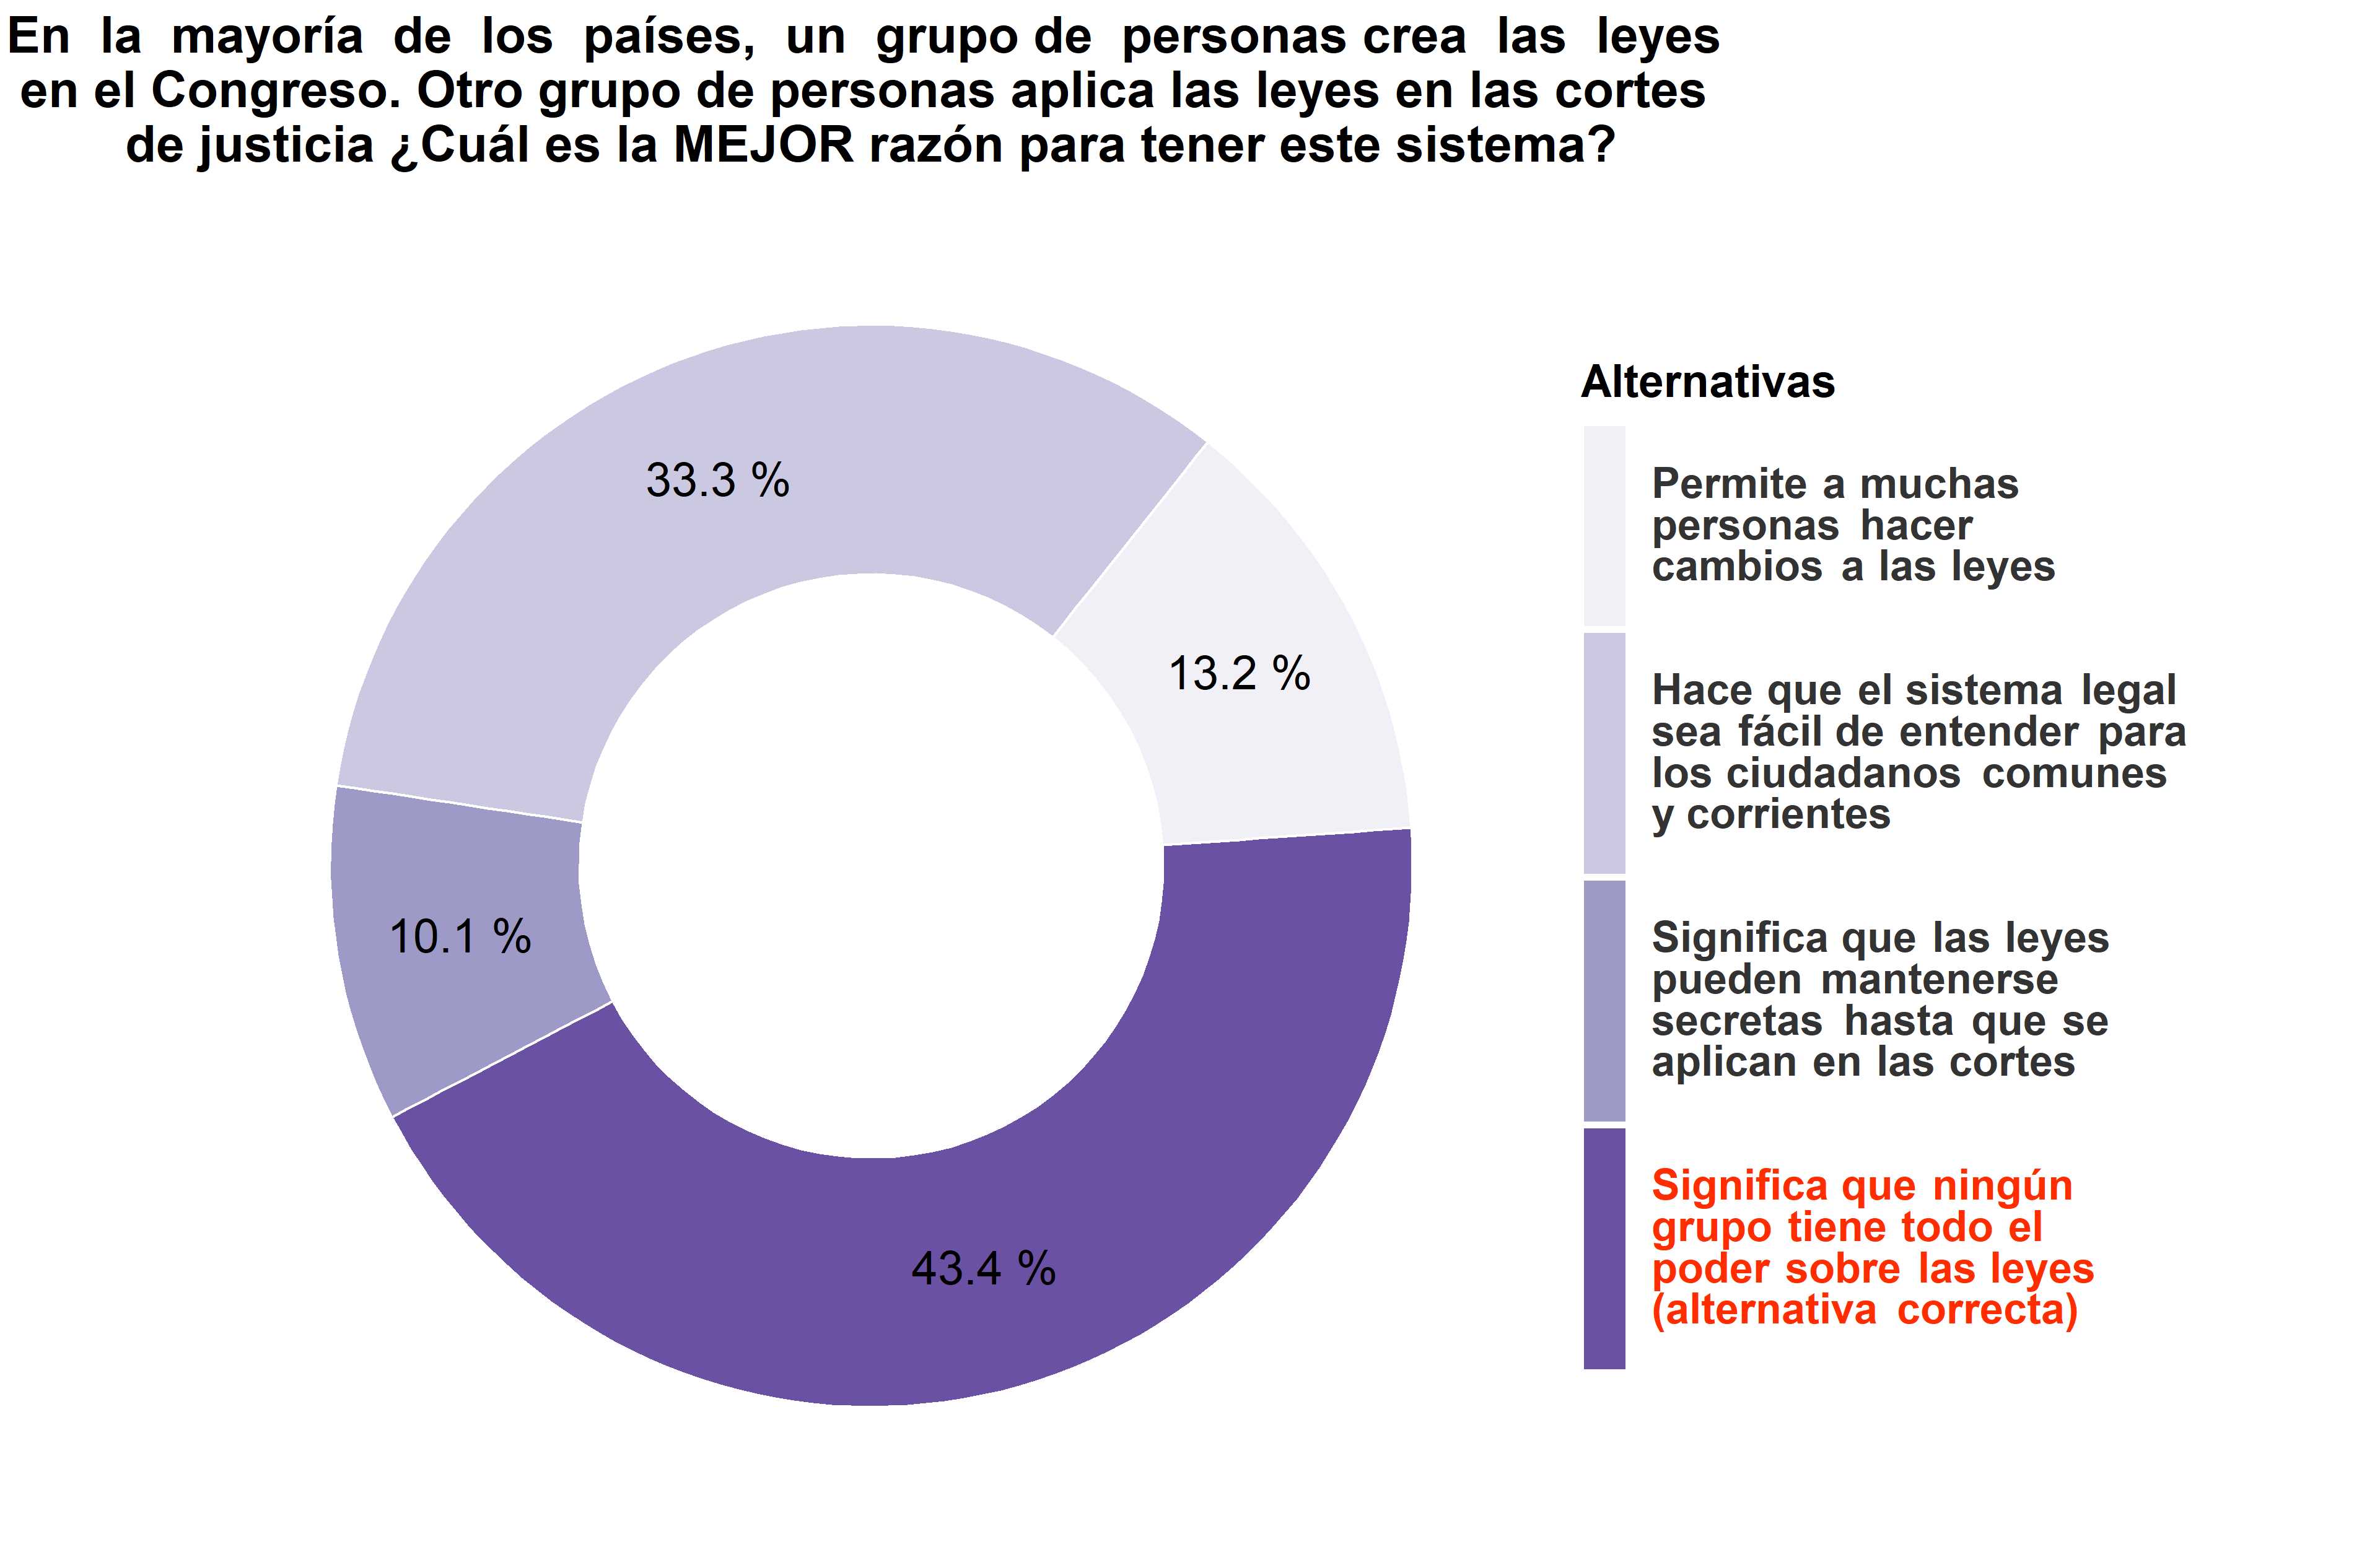
\includegraphics[width=52.49in]{images/ccivico_1} 

}

\caption{Razones para crear leyes en el Congreso}\label{fig:unnamed-chunk-2}
\end{figure}

Un 42\% de los estudiantes respondió correctamente la pregunta. Entre las alternativas incorrectas, hubo una que distrajó a parte importante de los estudiantes, concentrando el 34\% de las respuestas.

\begin{center}\rule{0.5\linewidth}{0.5pt}\end{center}

\hypertarget{segunda-pregunta}{%
\subsubsection{Segunda pregunta}\label{segunda-pregunta}}

\begin{center}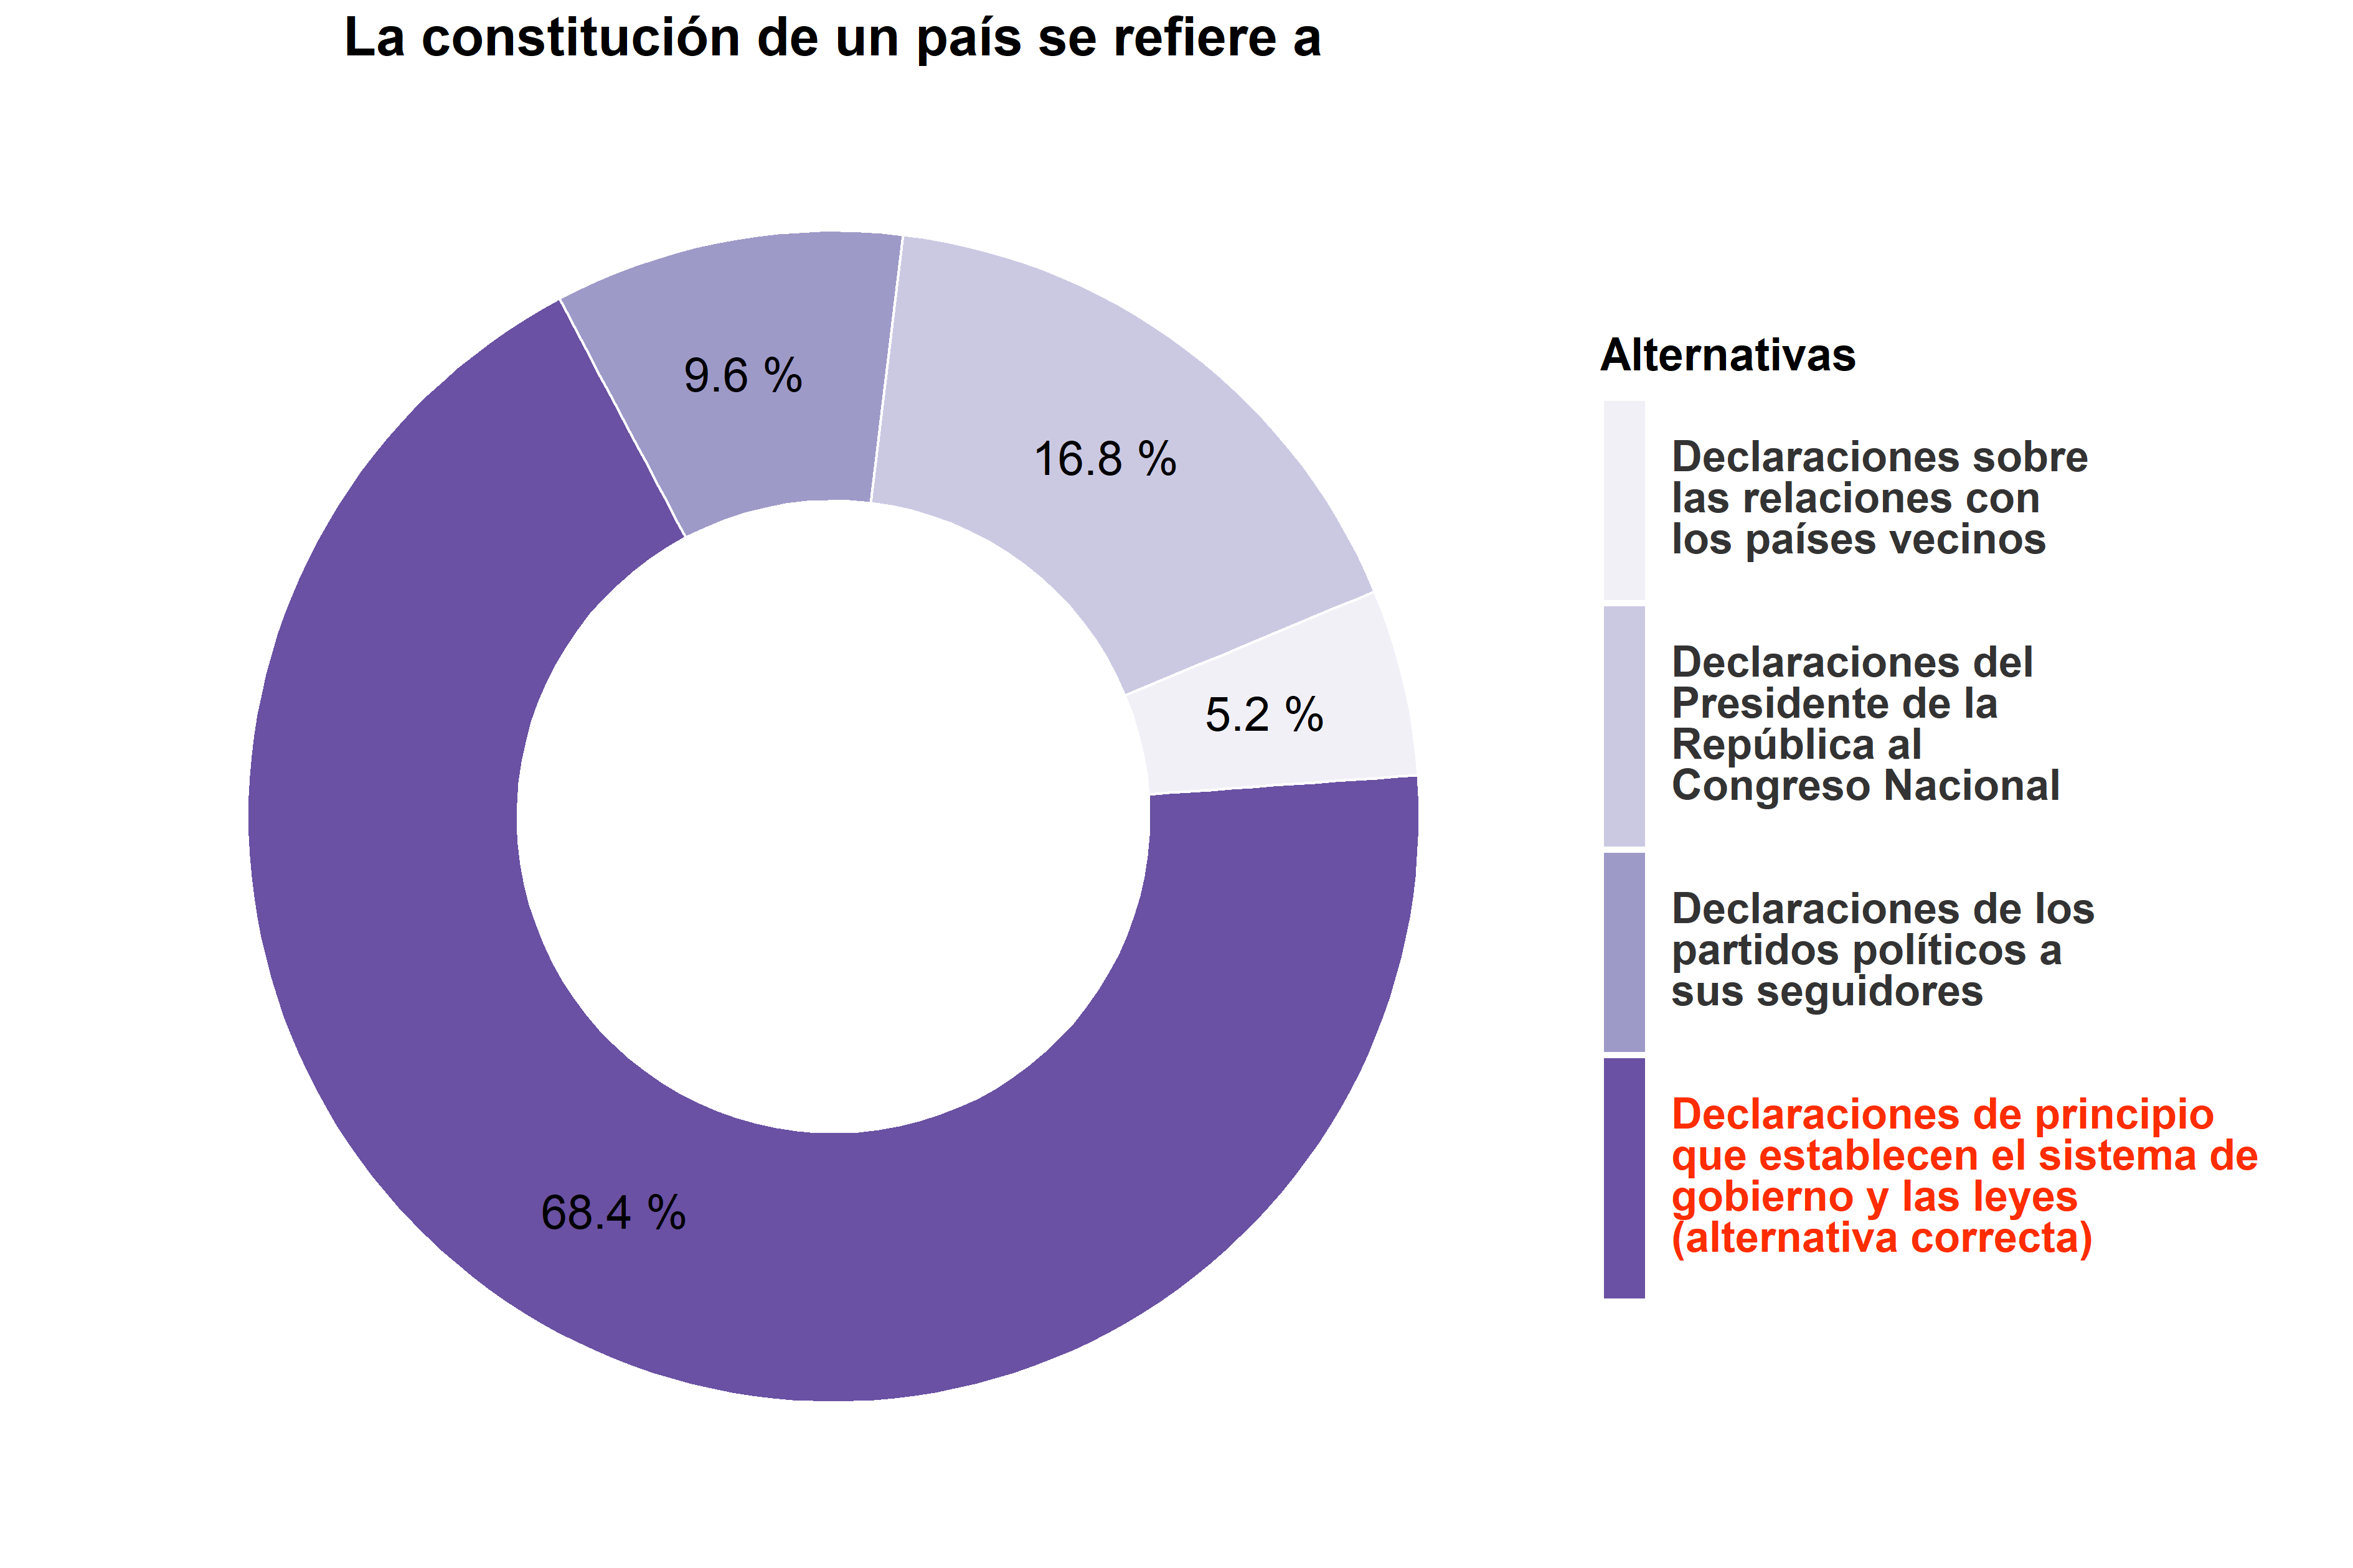
\includegraphics[width=52.49in]{images/ccivico_2} \end{center}

\hypertarget{tercera-pregunta}{%
\subsubsection{Tercera pregunta}\label{tercera-pregunta}}

\begin{center}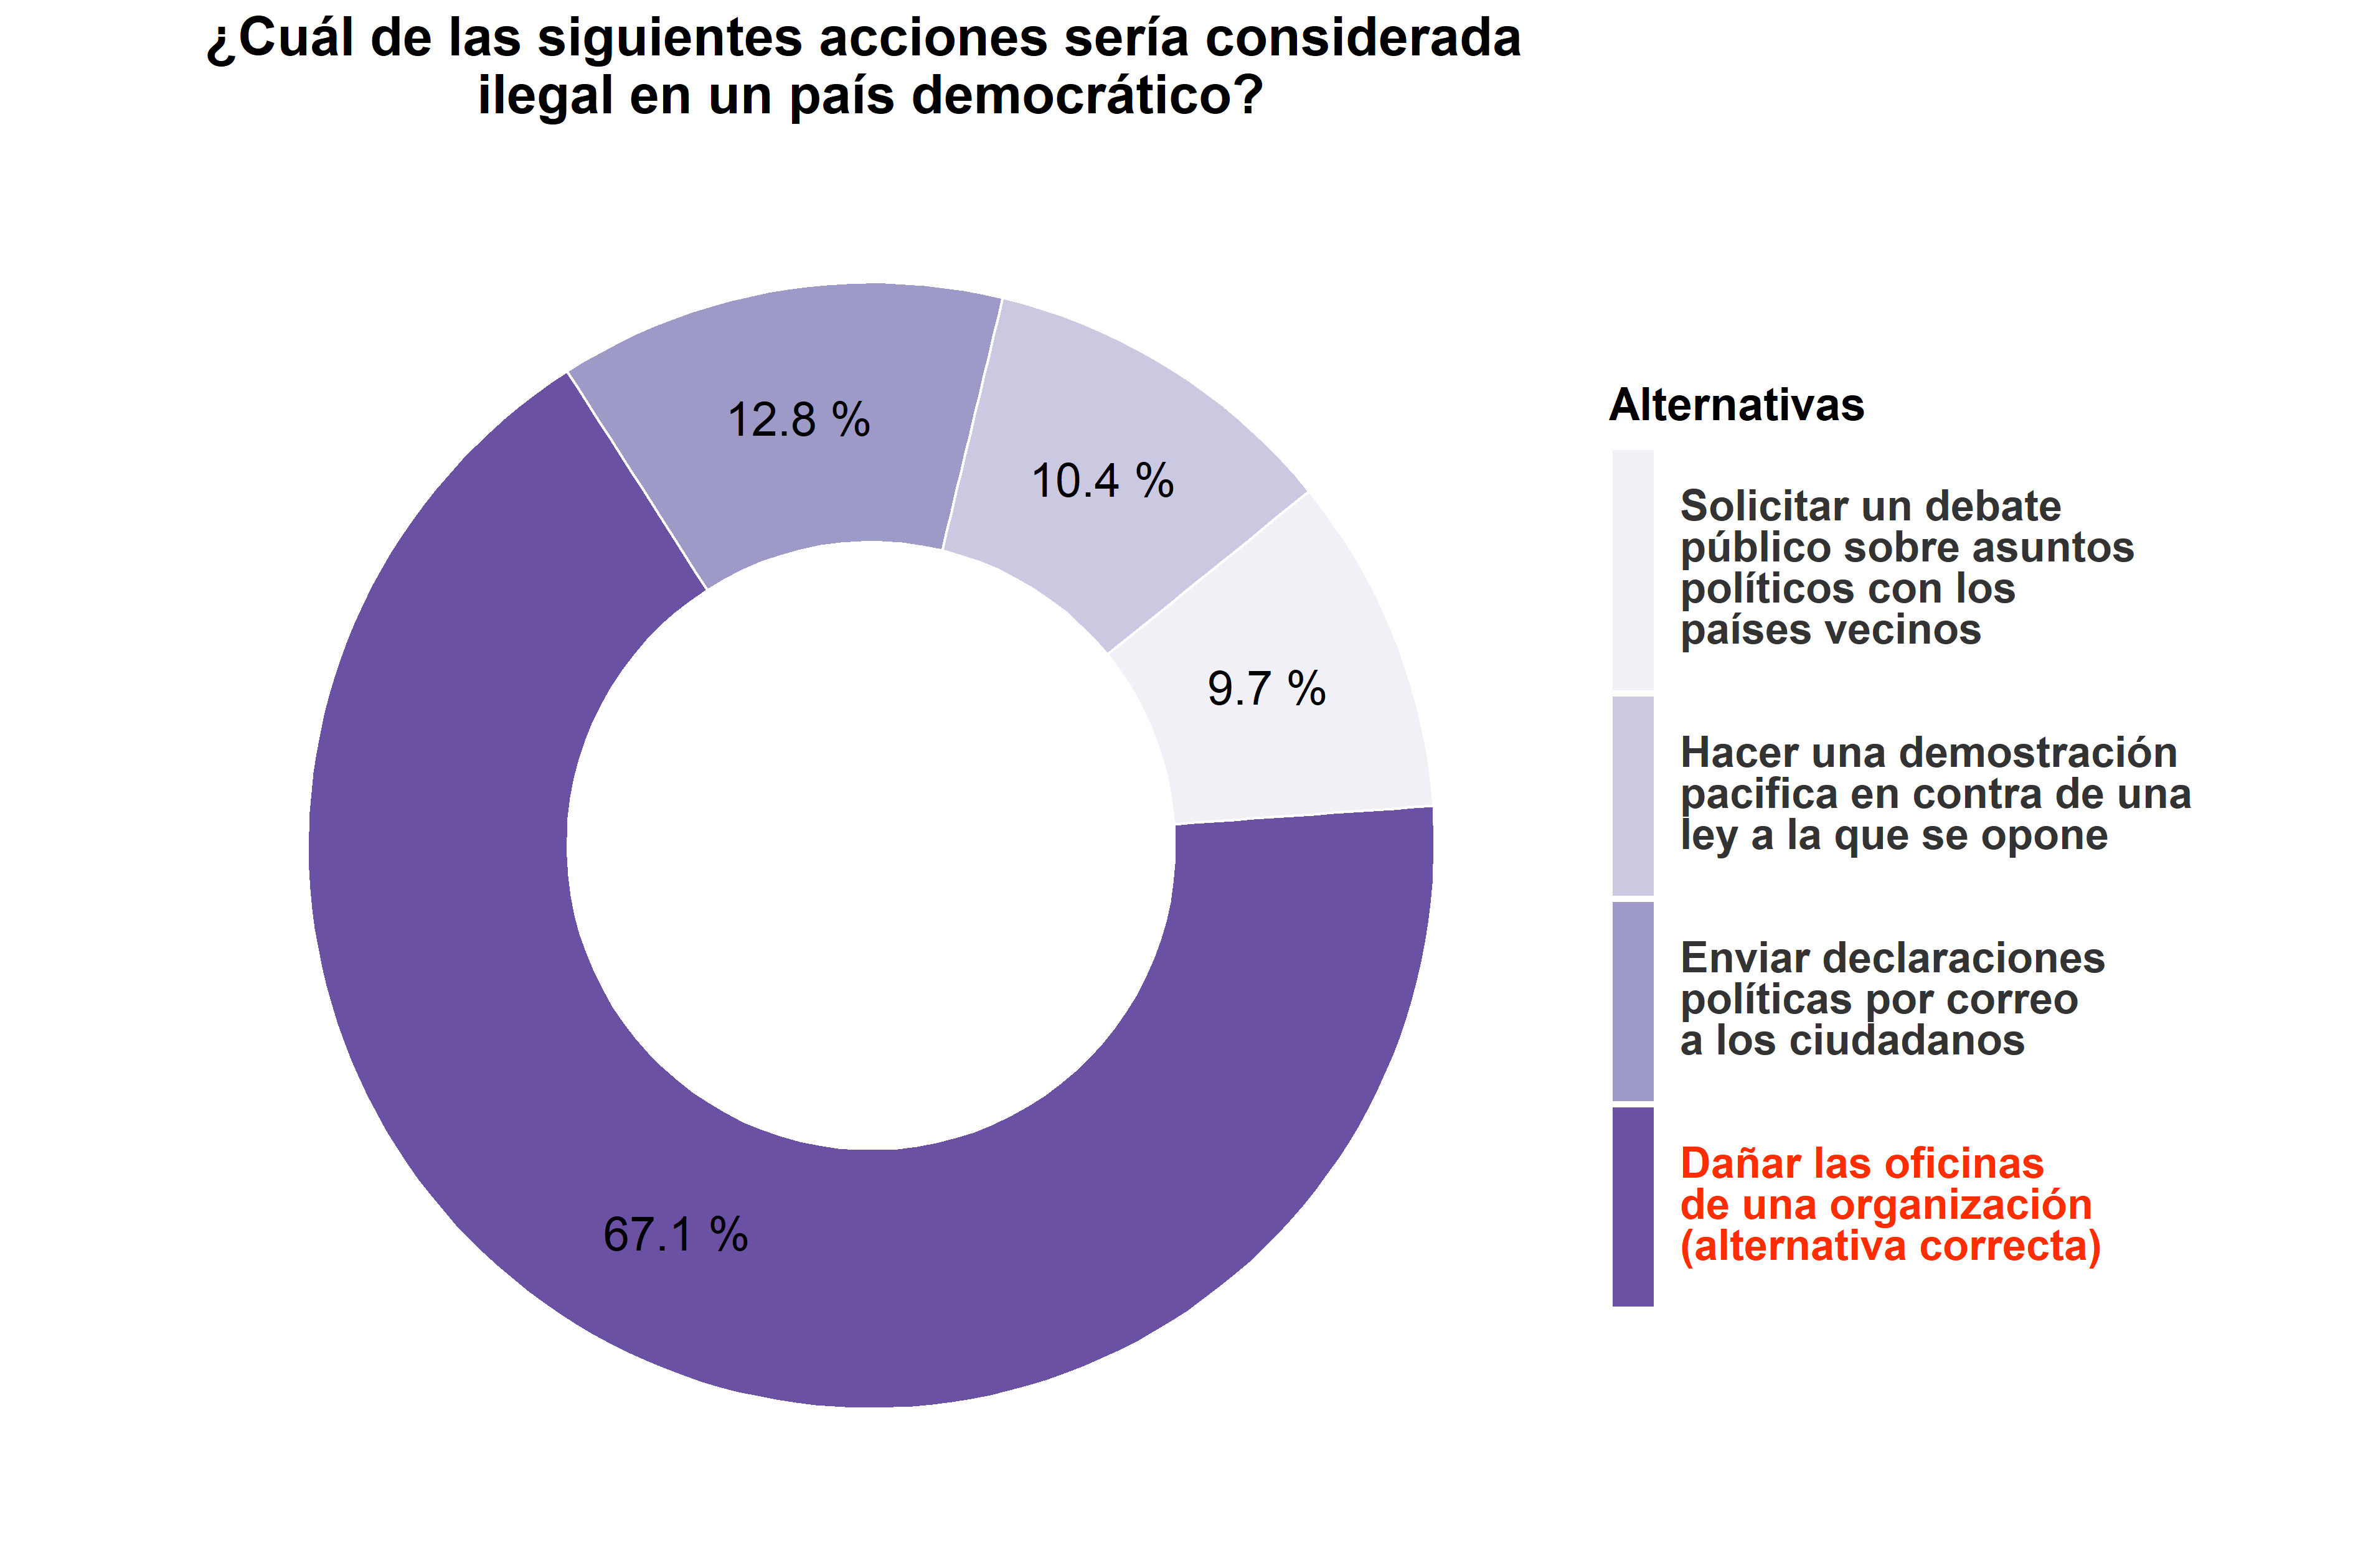
\includegraphics[width=52.49in]{images/ccivico_3} \end{center}

\hypertarget{cuarta-pregunta}{%
\subsubsection{Cuarta pregunta}\label{cuarta-pregunta}}

\begin{center}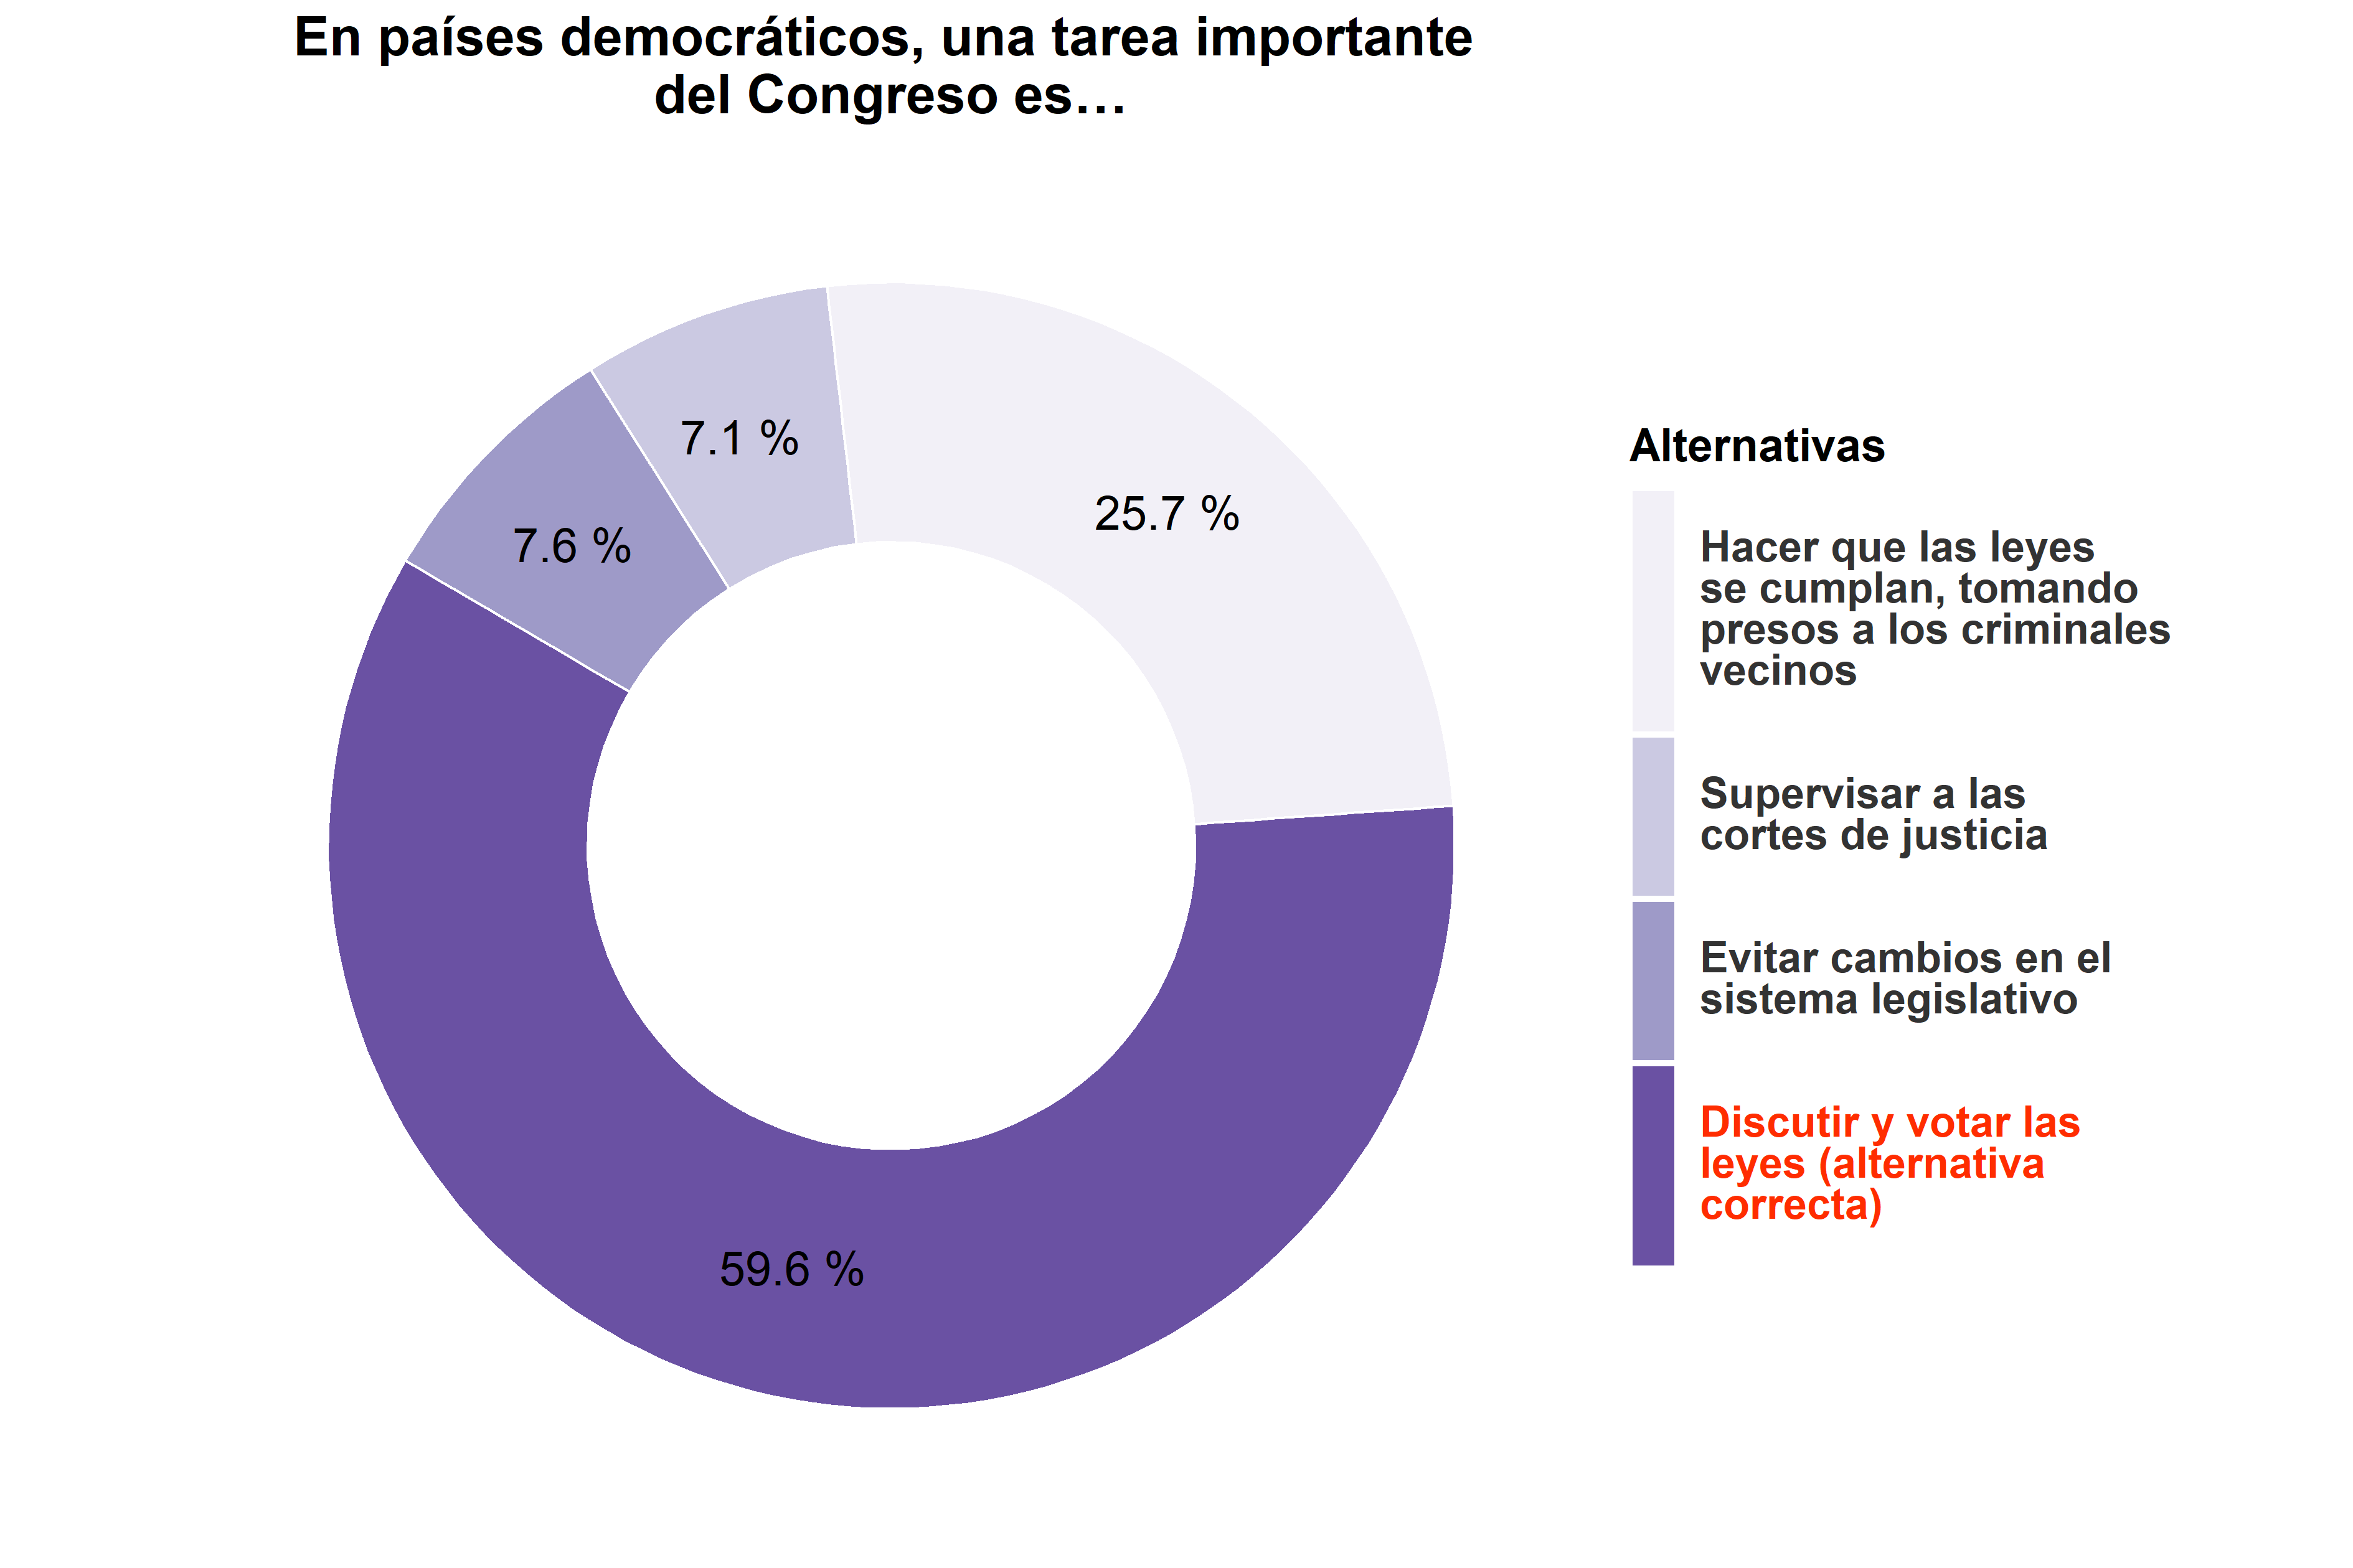
\includegraphics[width=52.49in]{images/ccivico_4} \end{center}

\hypertarget{quinta-pregunta}{%
\subsubsection{Quinta pregunta}\label{quinta-pregunta}}

\begin{center}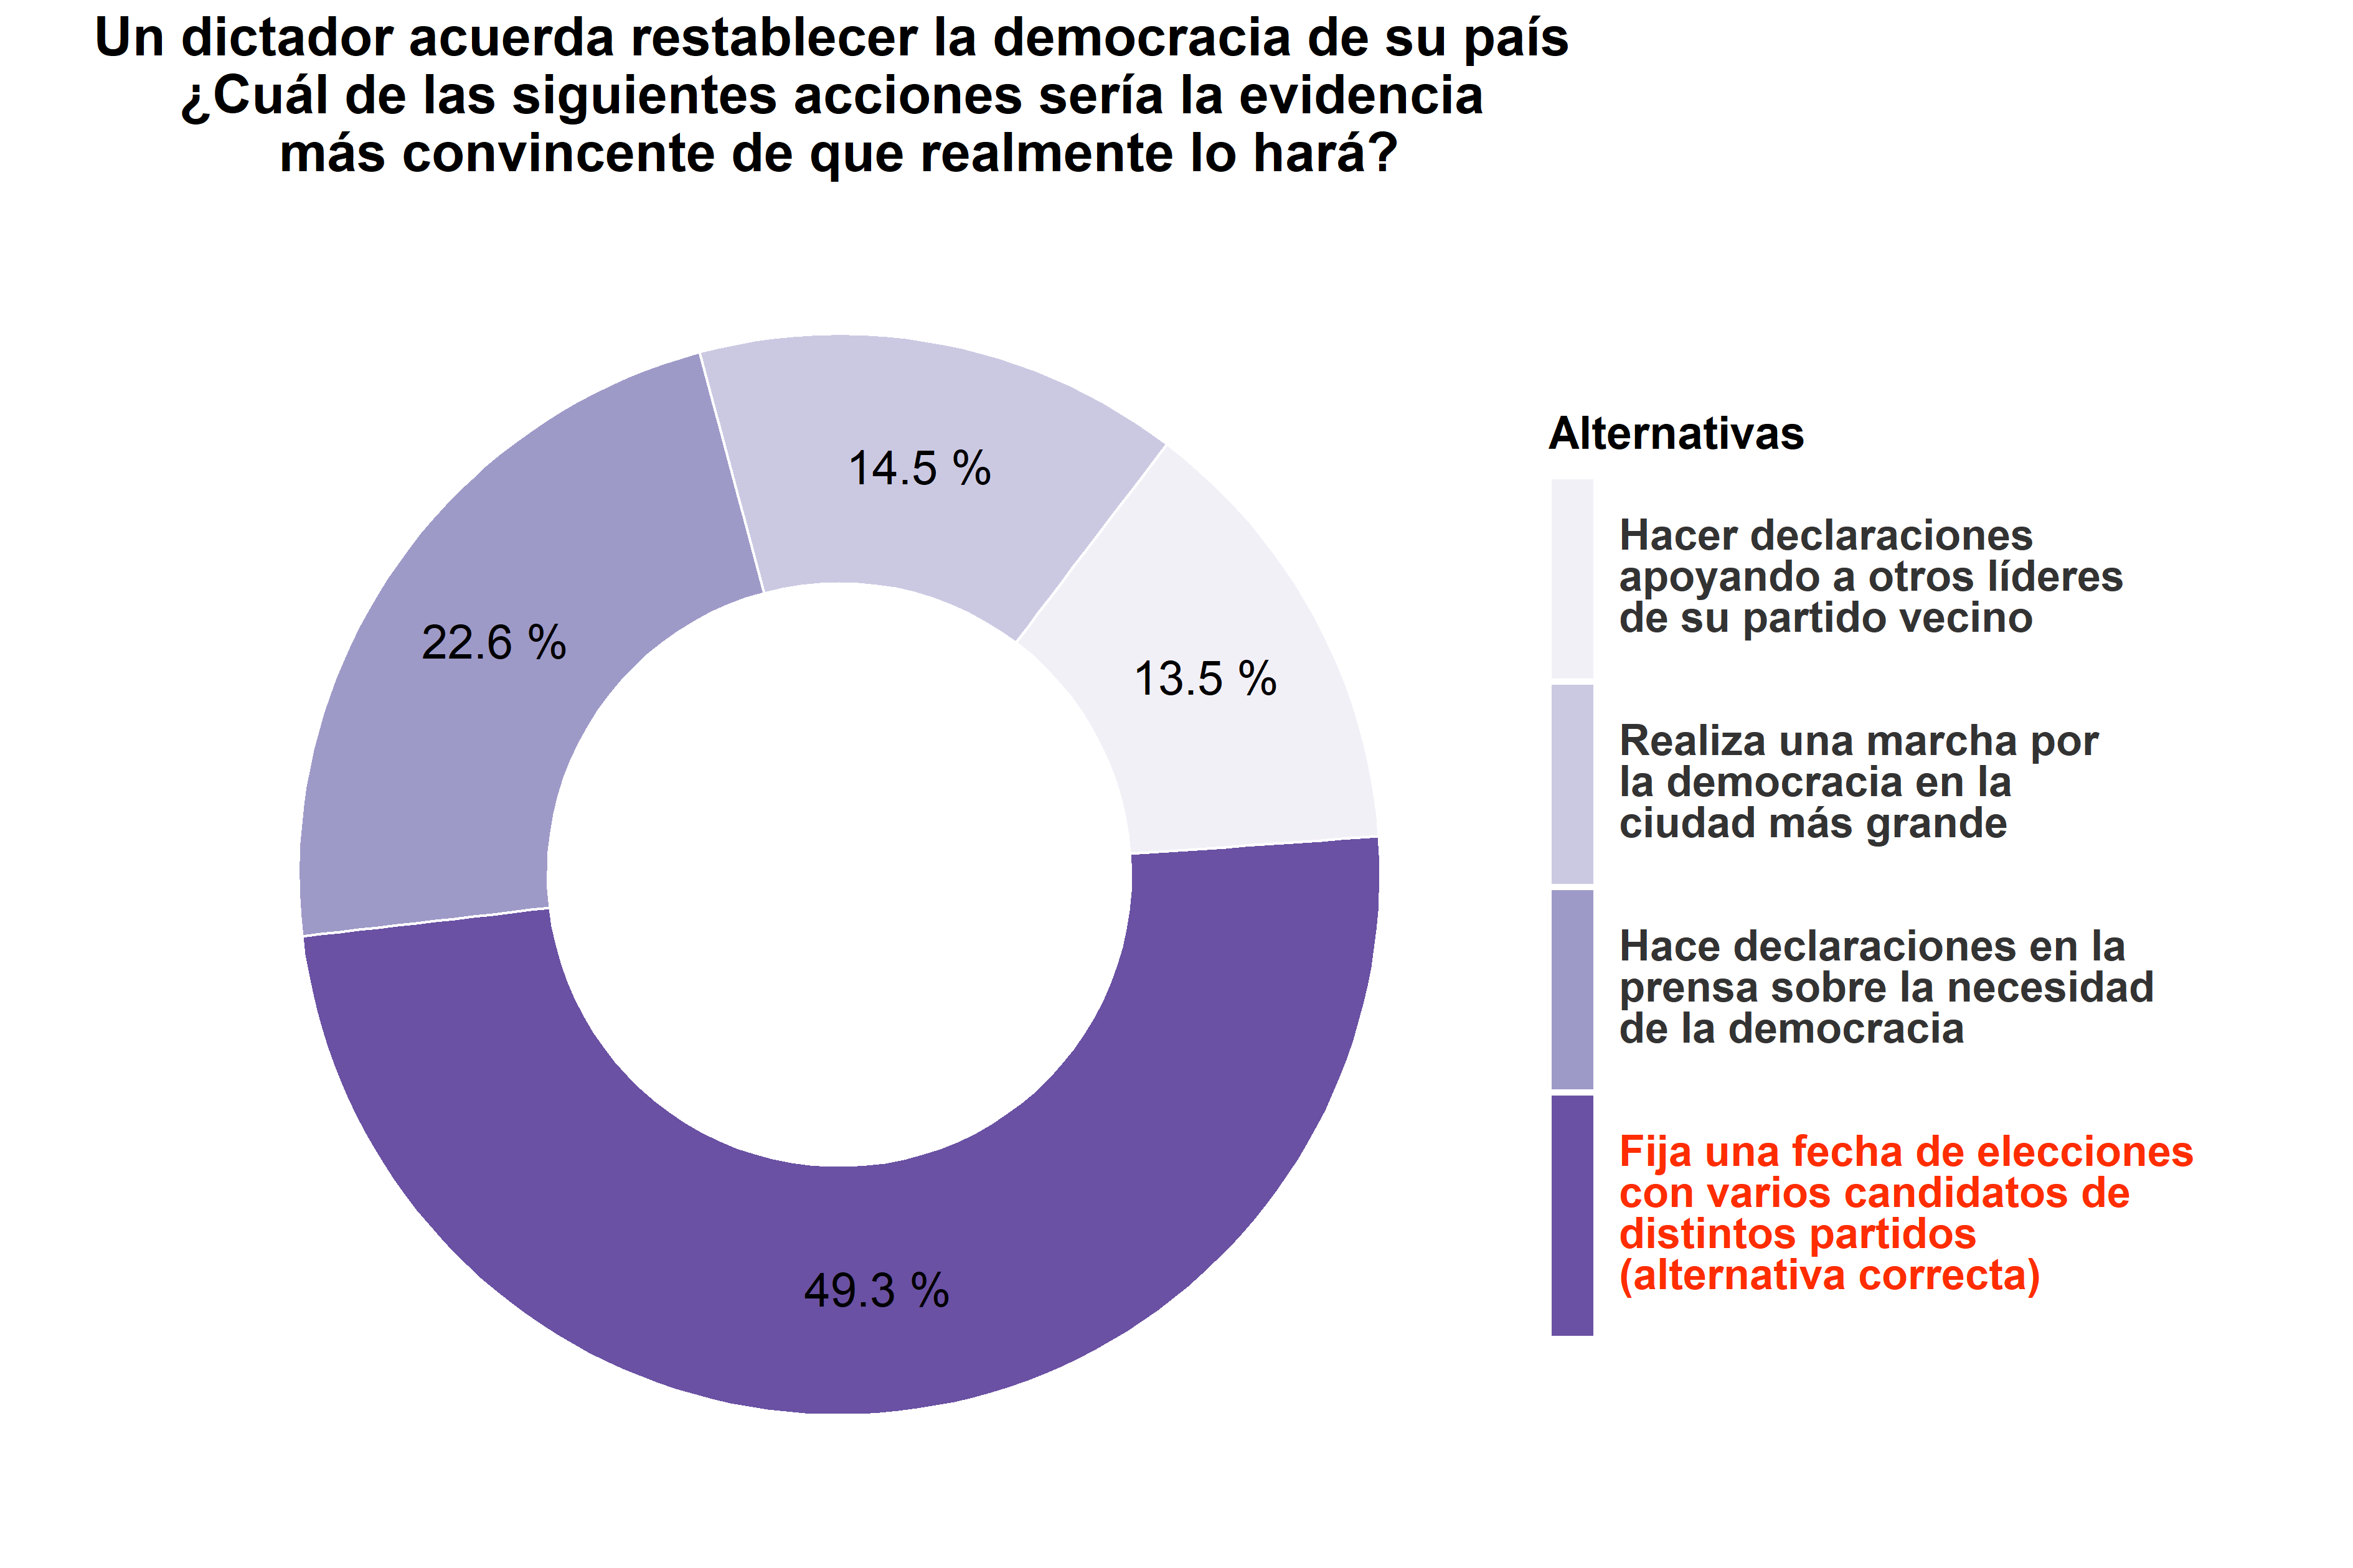
\includegraphics[width=52.49in]{images/ccivico_5} \end{center}

\hypertarget{sexta-pregunta}{%
\subsubsection{Sexta pregunta}\label{sexta-pregunta}}

\begin{center}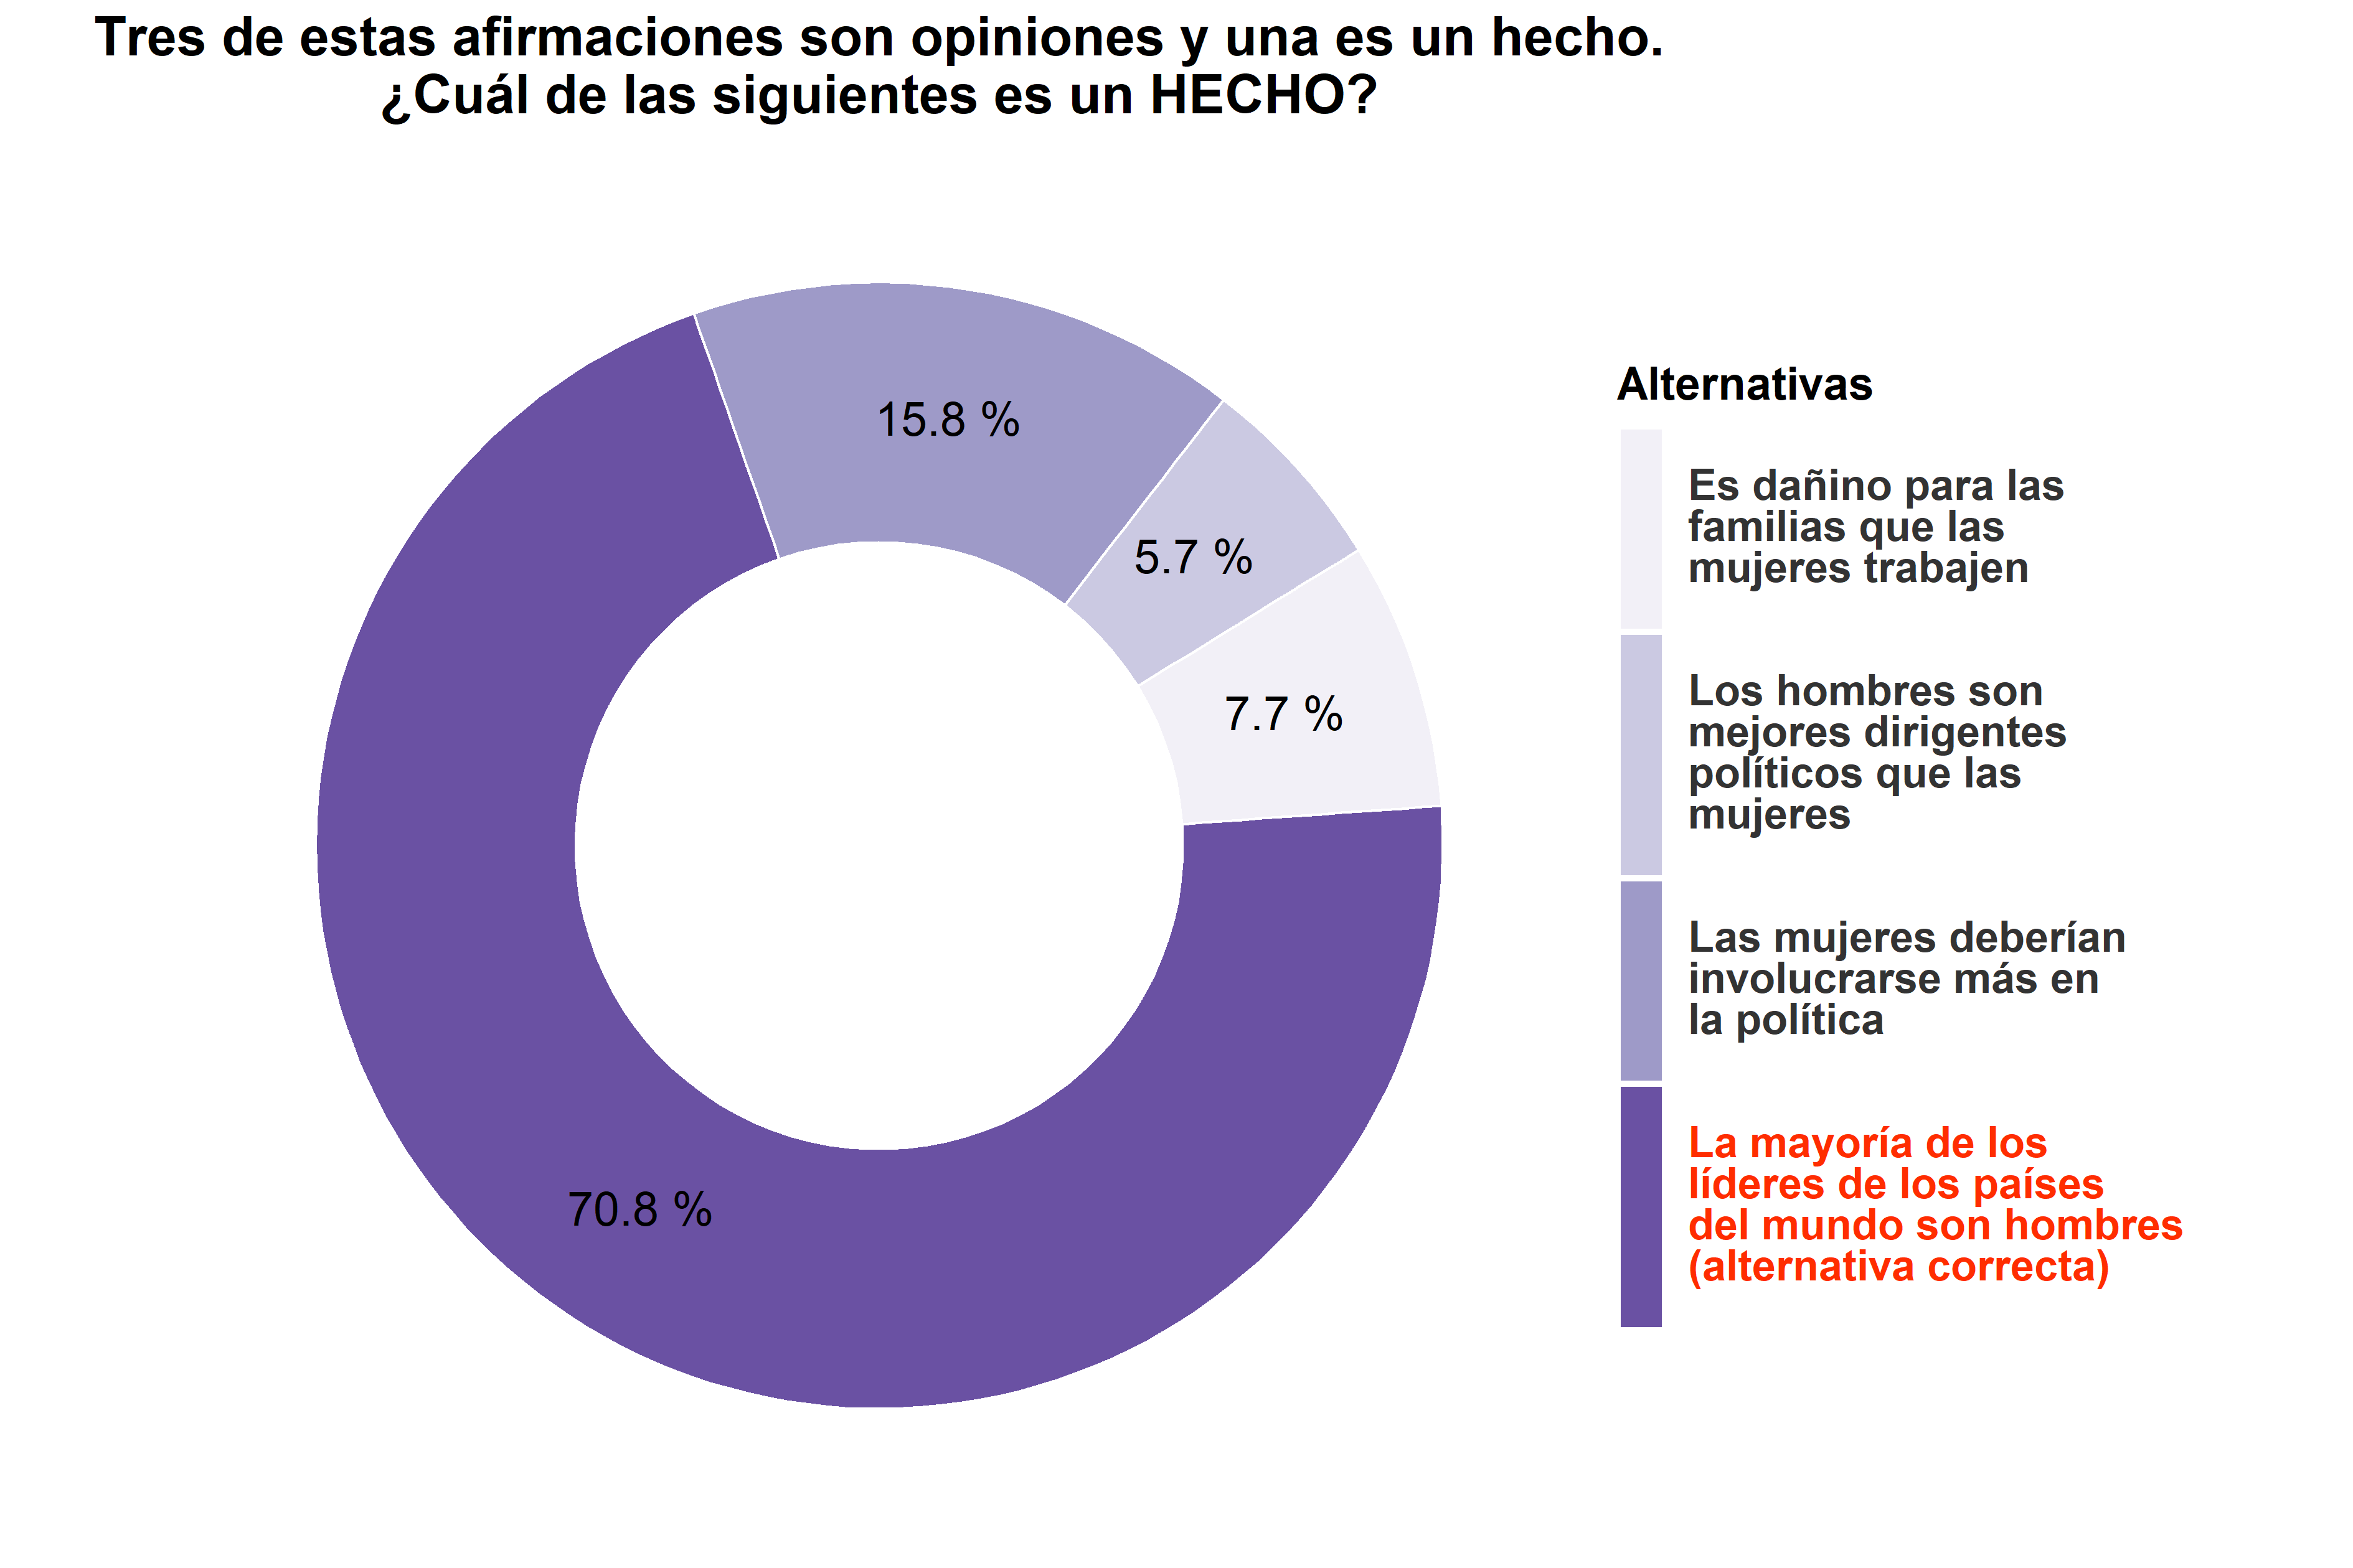
\includegraphics[width=52.49in]{images/ccivico_6} \end{center}

\hypertarget{suxe9ptima-pregunta}{%
\subsubsection{Séptima pregunta}\label{suxe9ptima-pregunta}}

\begin{center}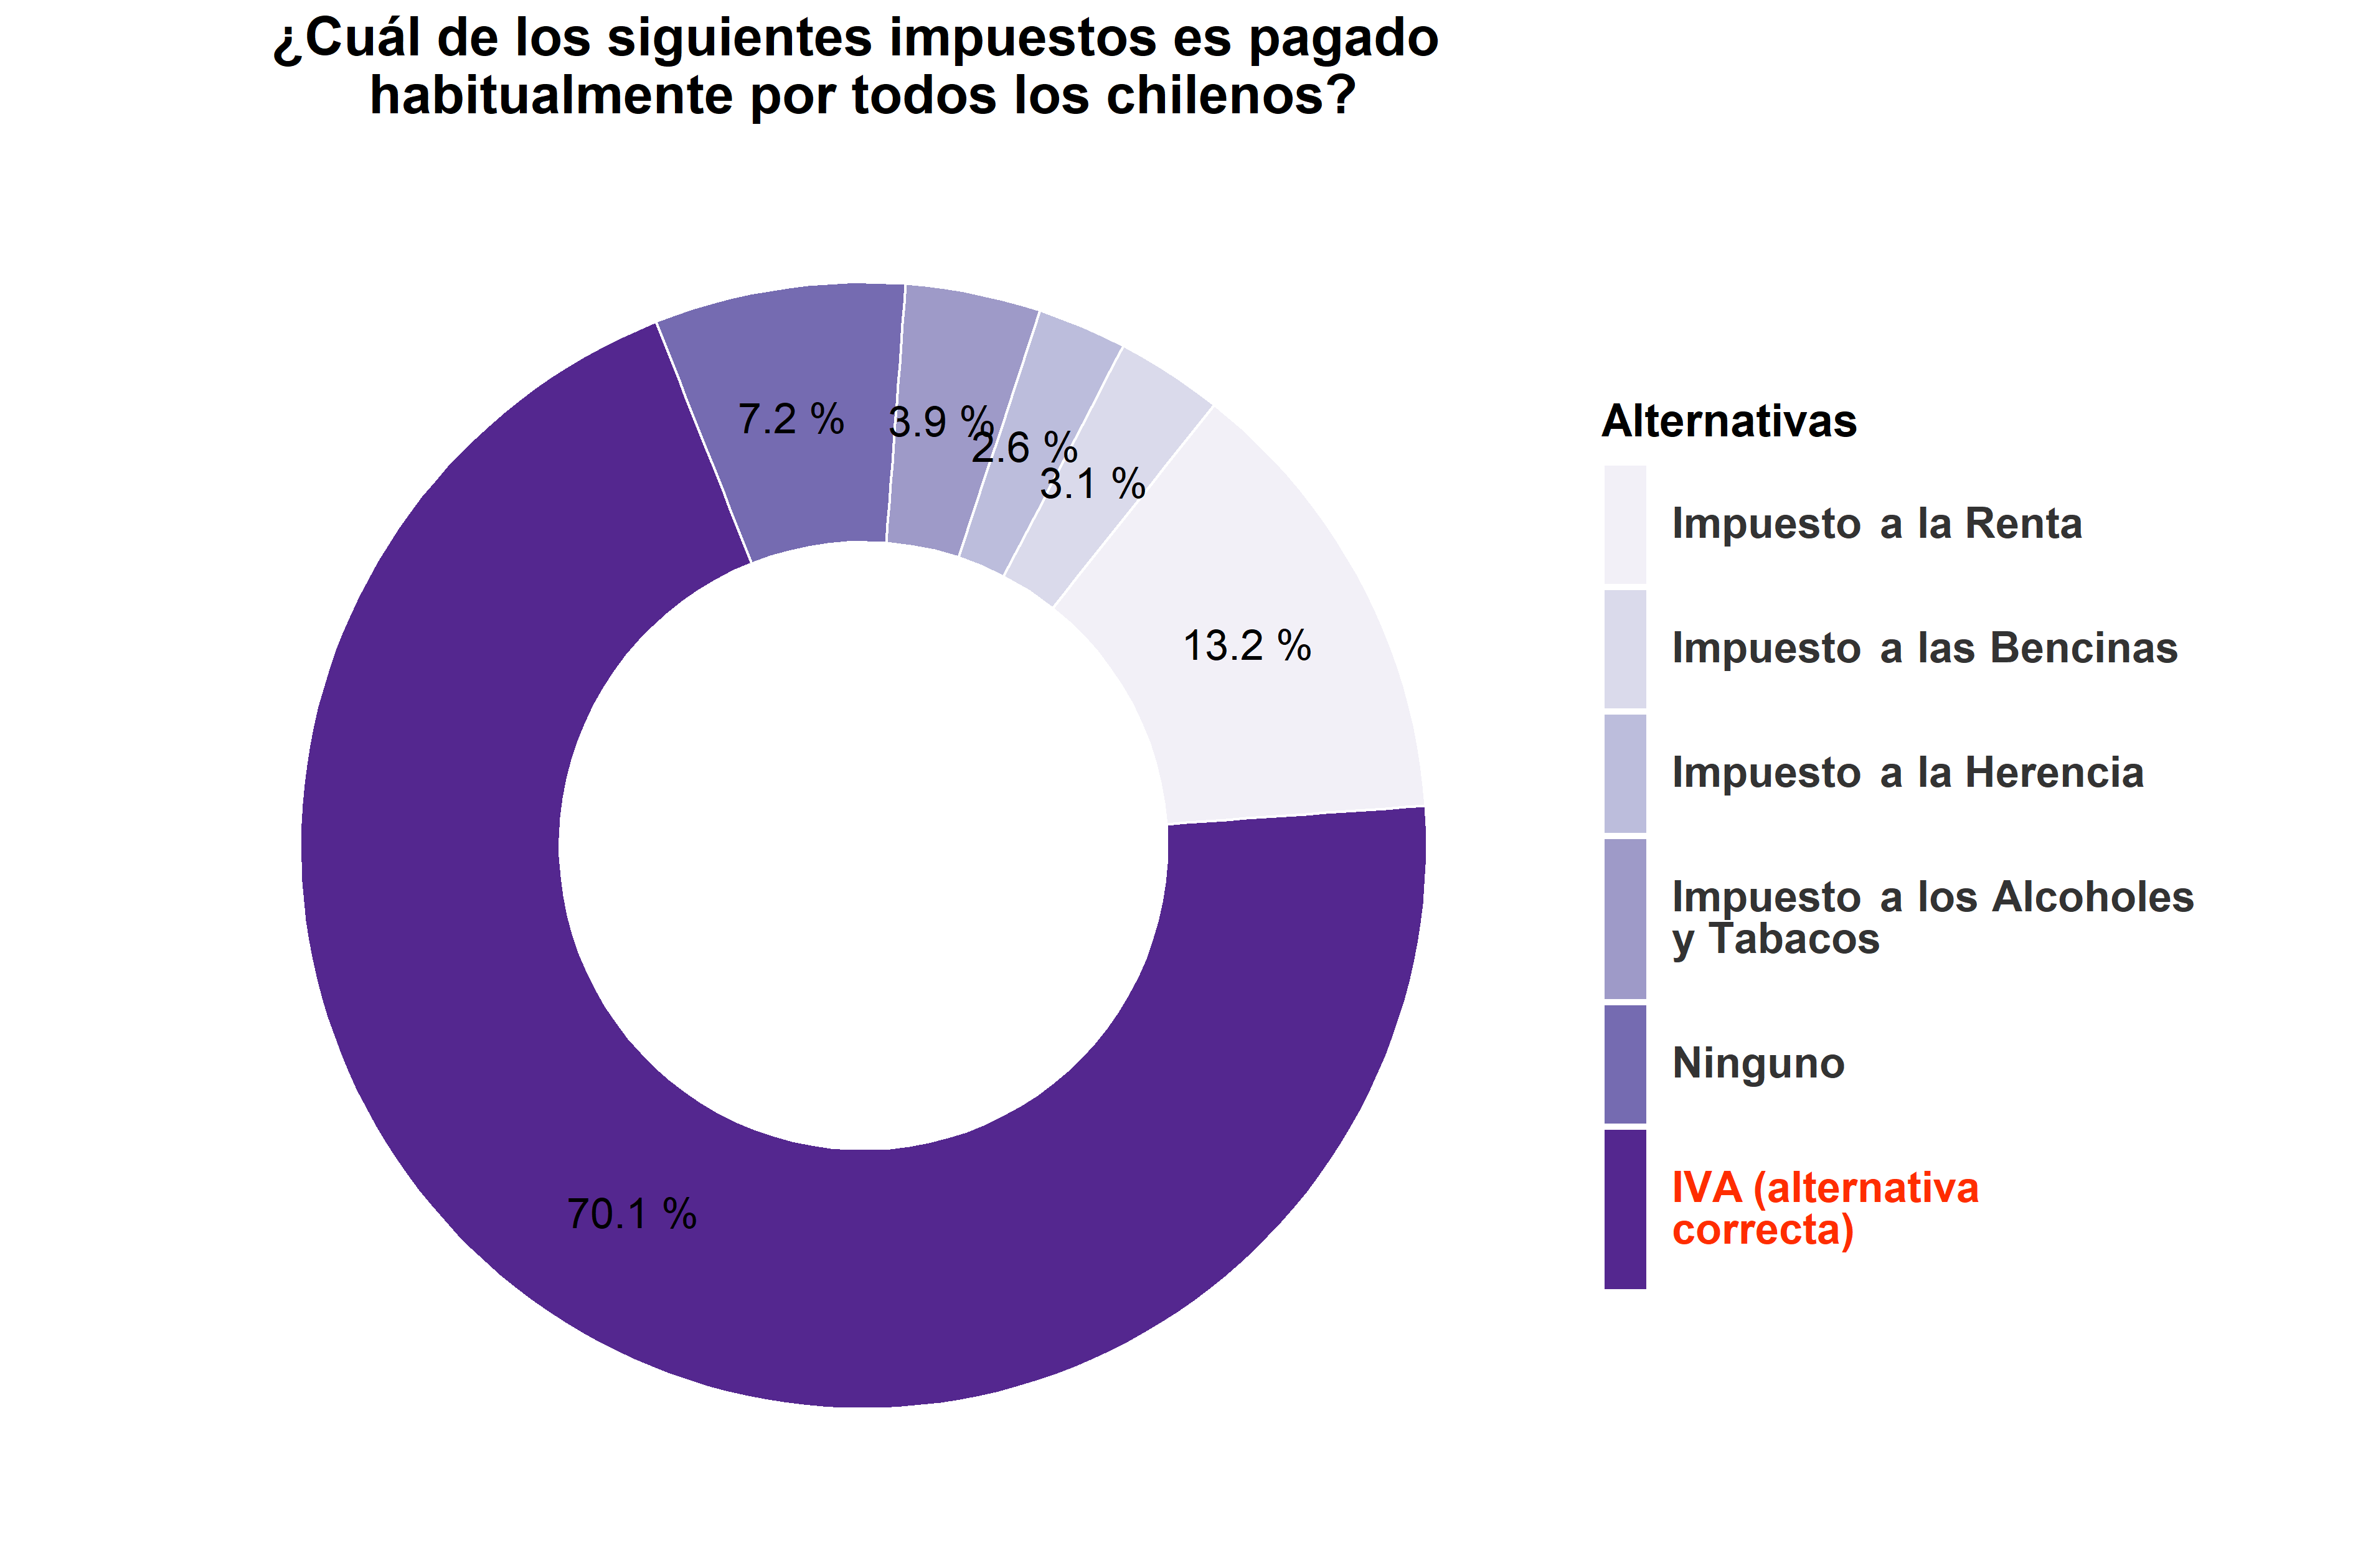
\includegraphics[width=52.49in]{images/ccivico_7} \end{center}

\hypertarget{octava-pregunta}{%
\subsubsection{Octava pregunta}\label{octava-pregunta}}

\begin{center}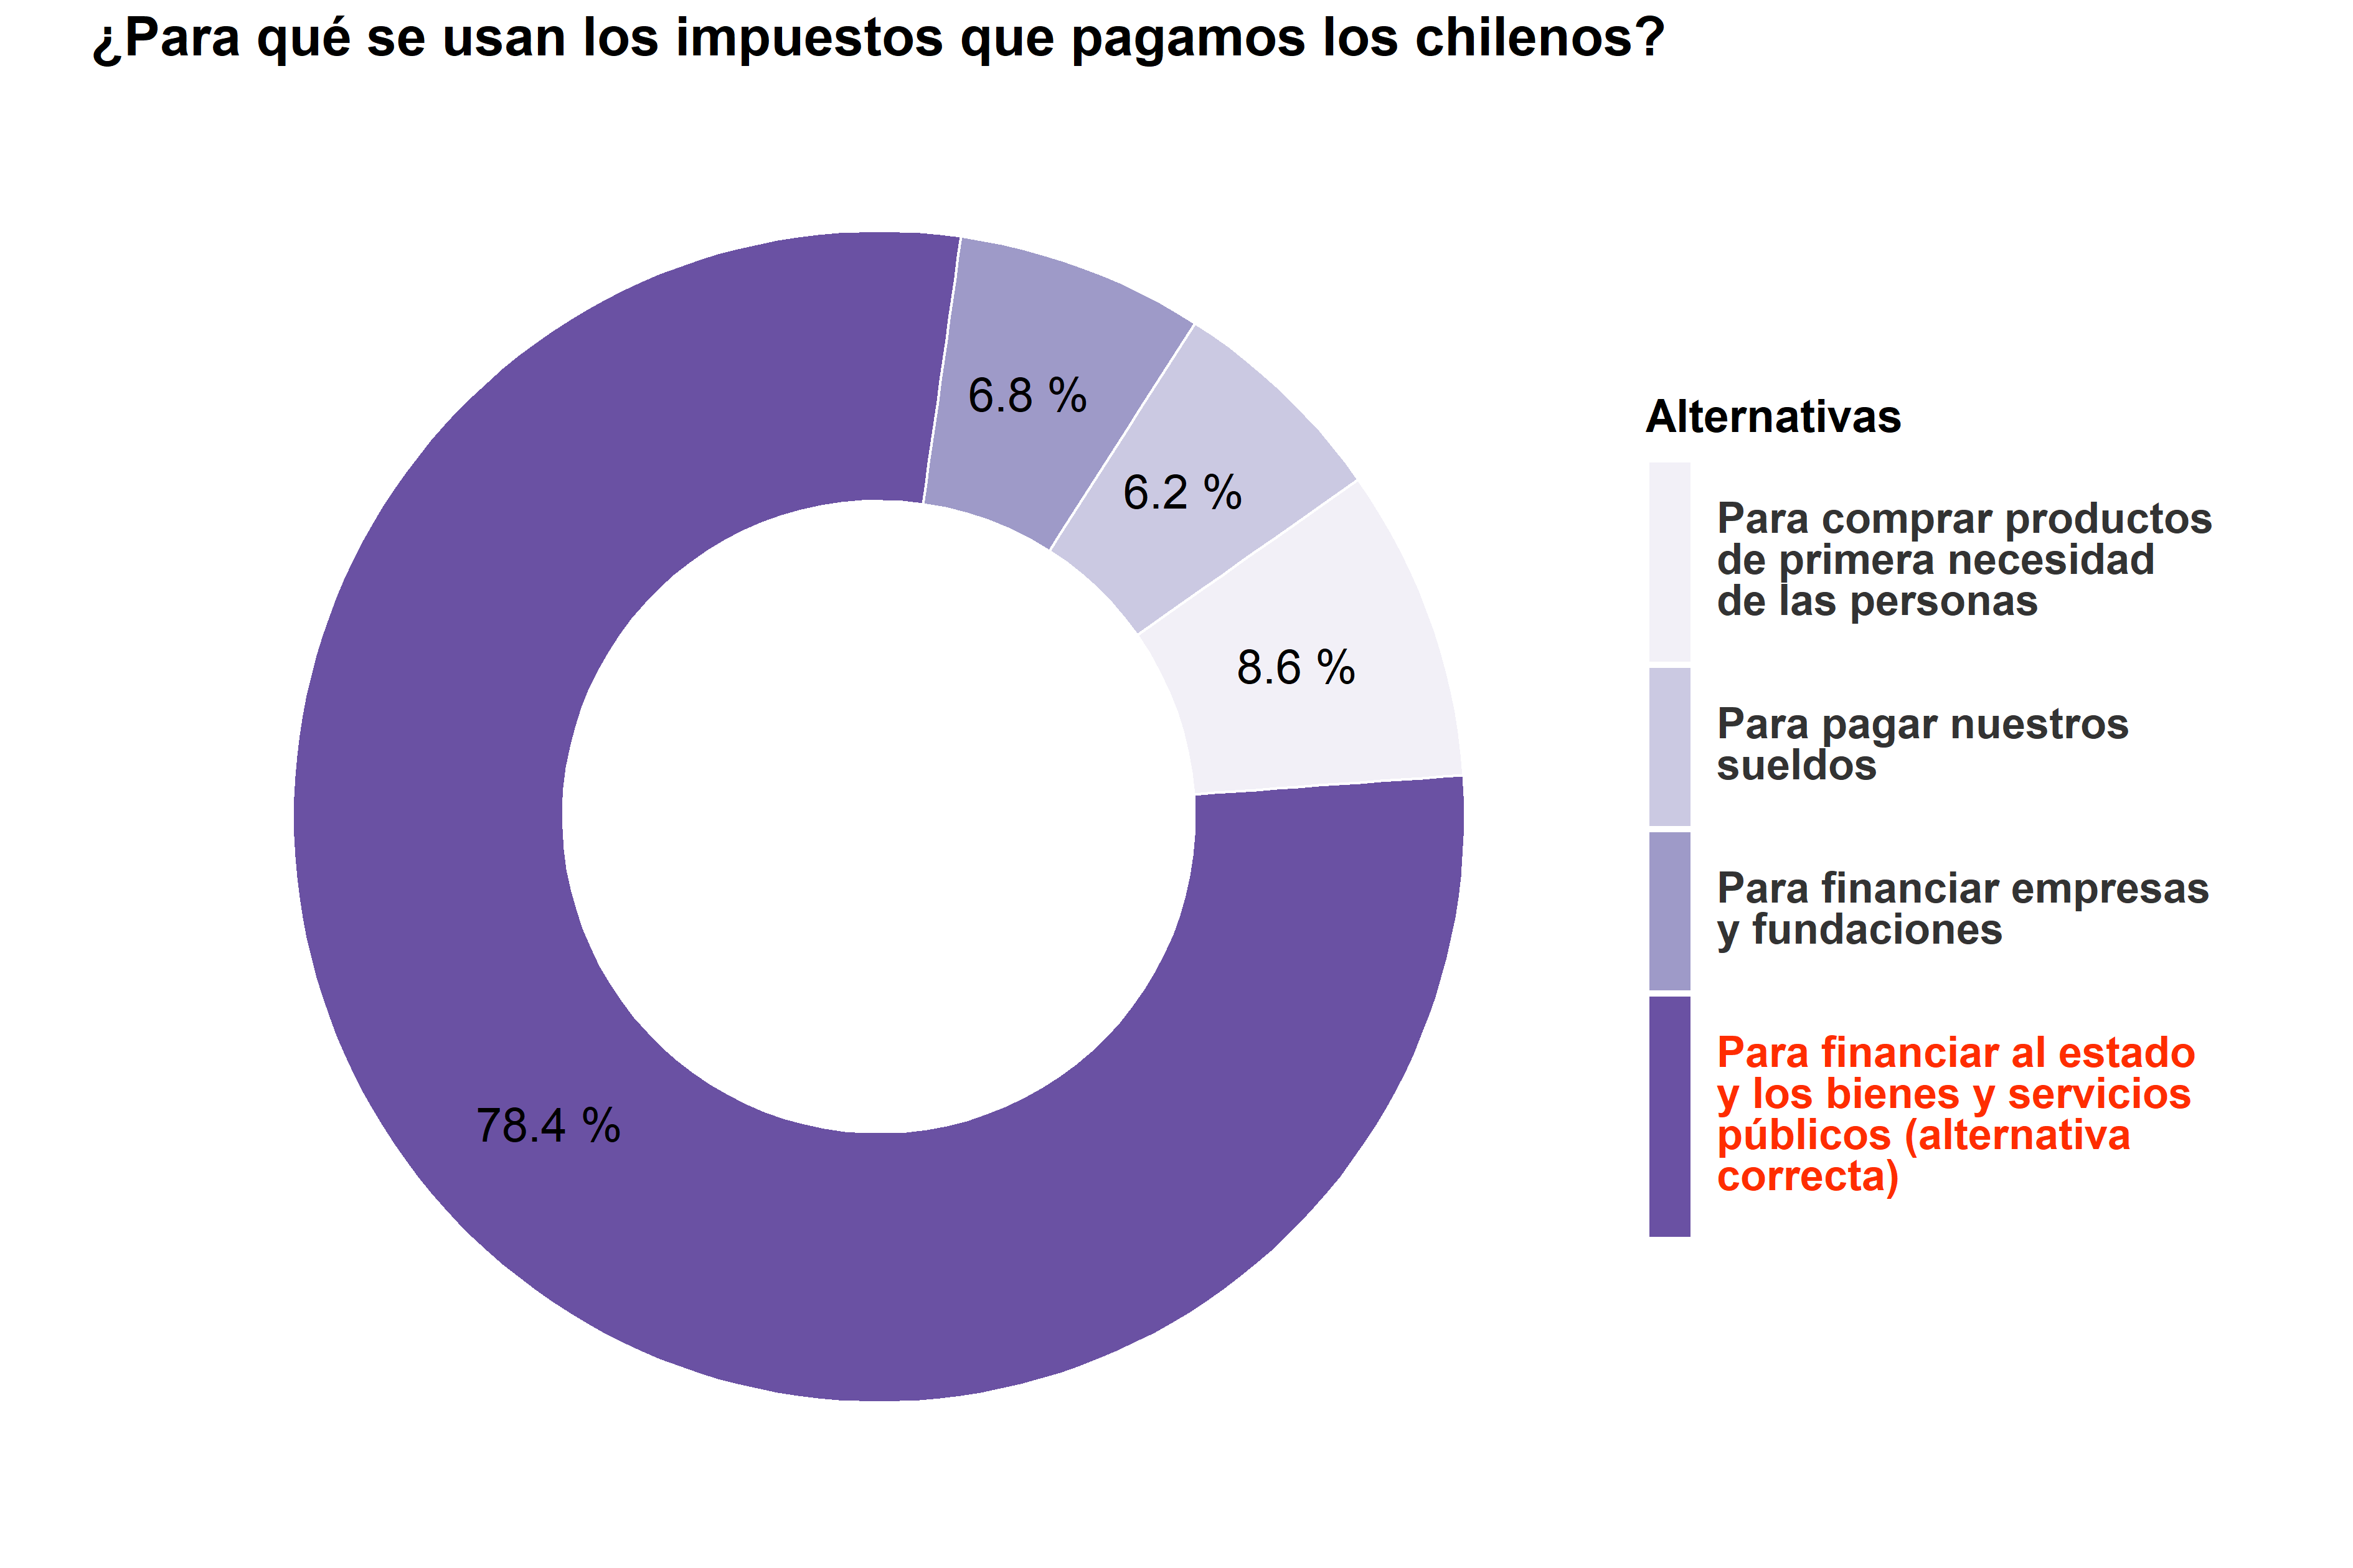
\includegraphics[width=52.49in]{images/ccivico_8} \end{center}

\hypertarget{novena-pregunta}{%
\subsubsection{Novena pregunta}\label{novena-pregunta}}

\begin{center}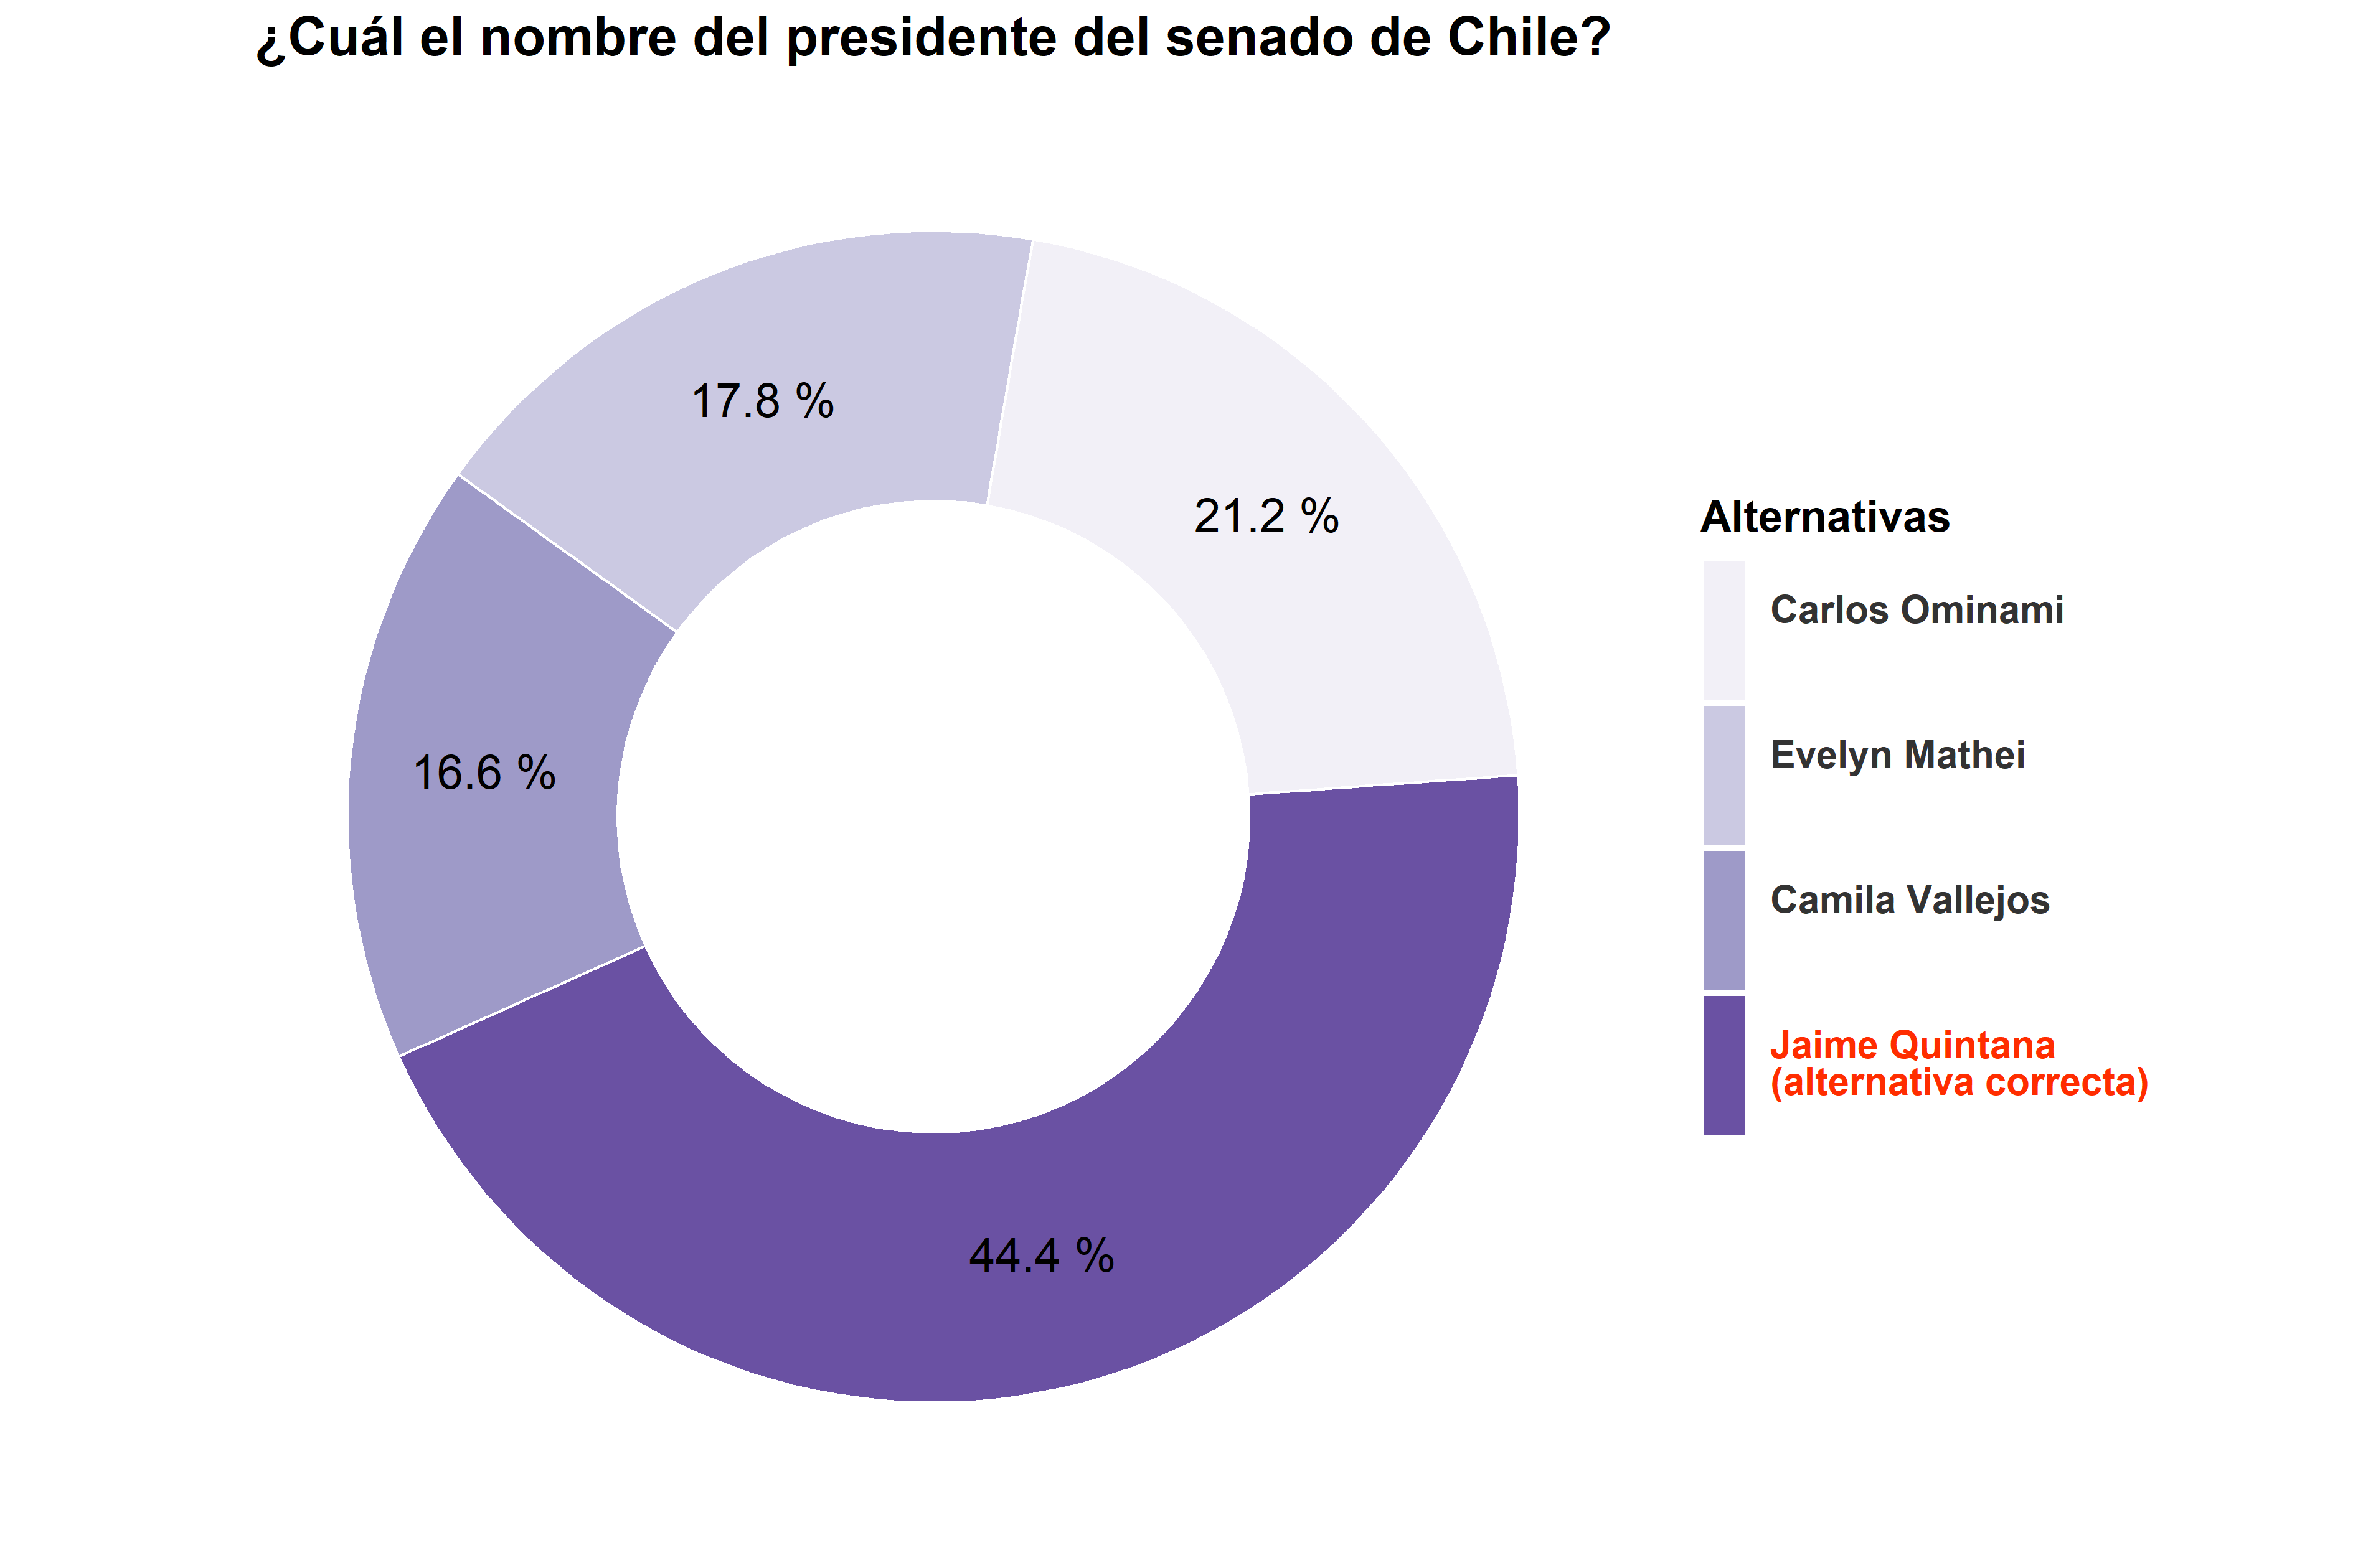
\includegraphics[width=52.49in]{images/ccivico_9} \end{center}

\hypertarget{duxe9cima-pregunta}{%
\subsubsection{Décima pregunta}\label{duxe9cima-pregunta}}

\begin{center}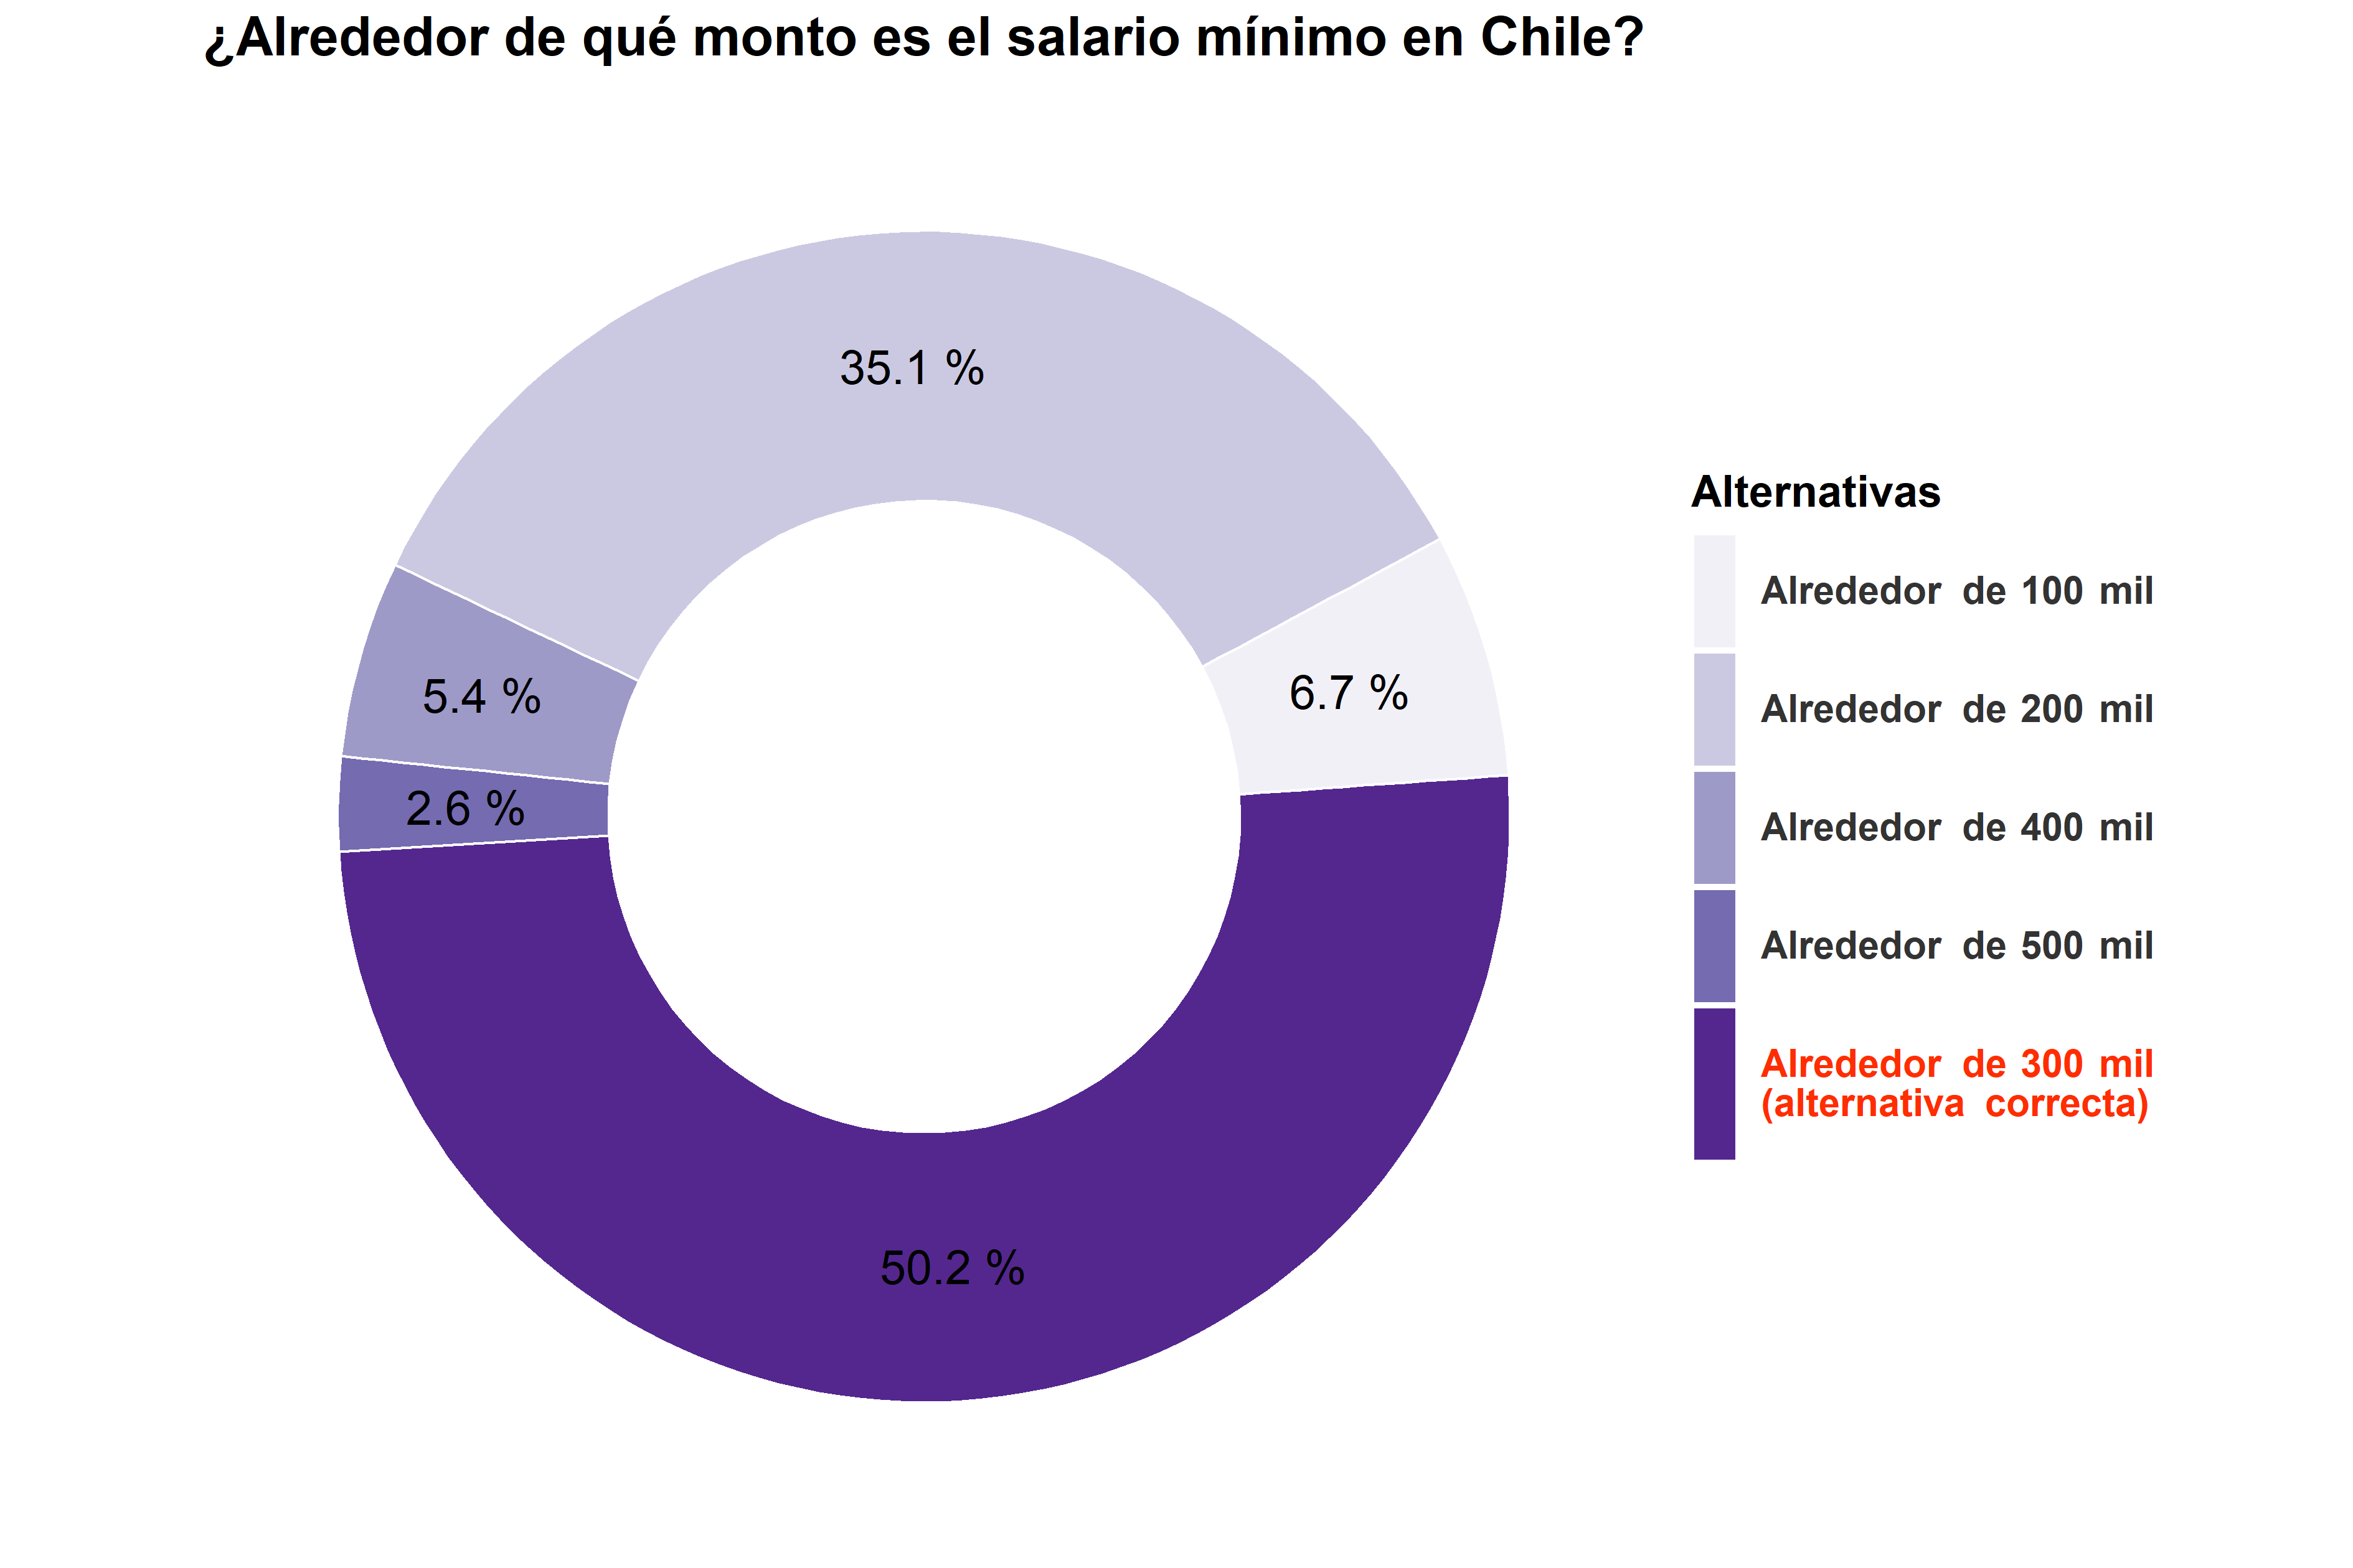
\includegraphics[width=52.49in]{images/ccivico_10} \end{center}

\hypertarget{unduxe9cima-pregunta}{%
\subsubsection{Undécima pregunta}\label{unduxe9cima-pregunta}}

\begin{center}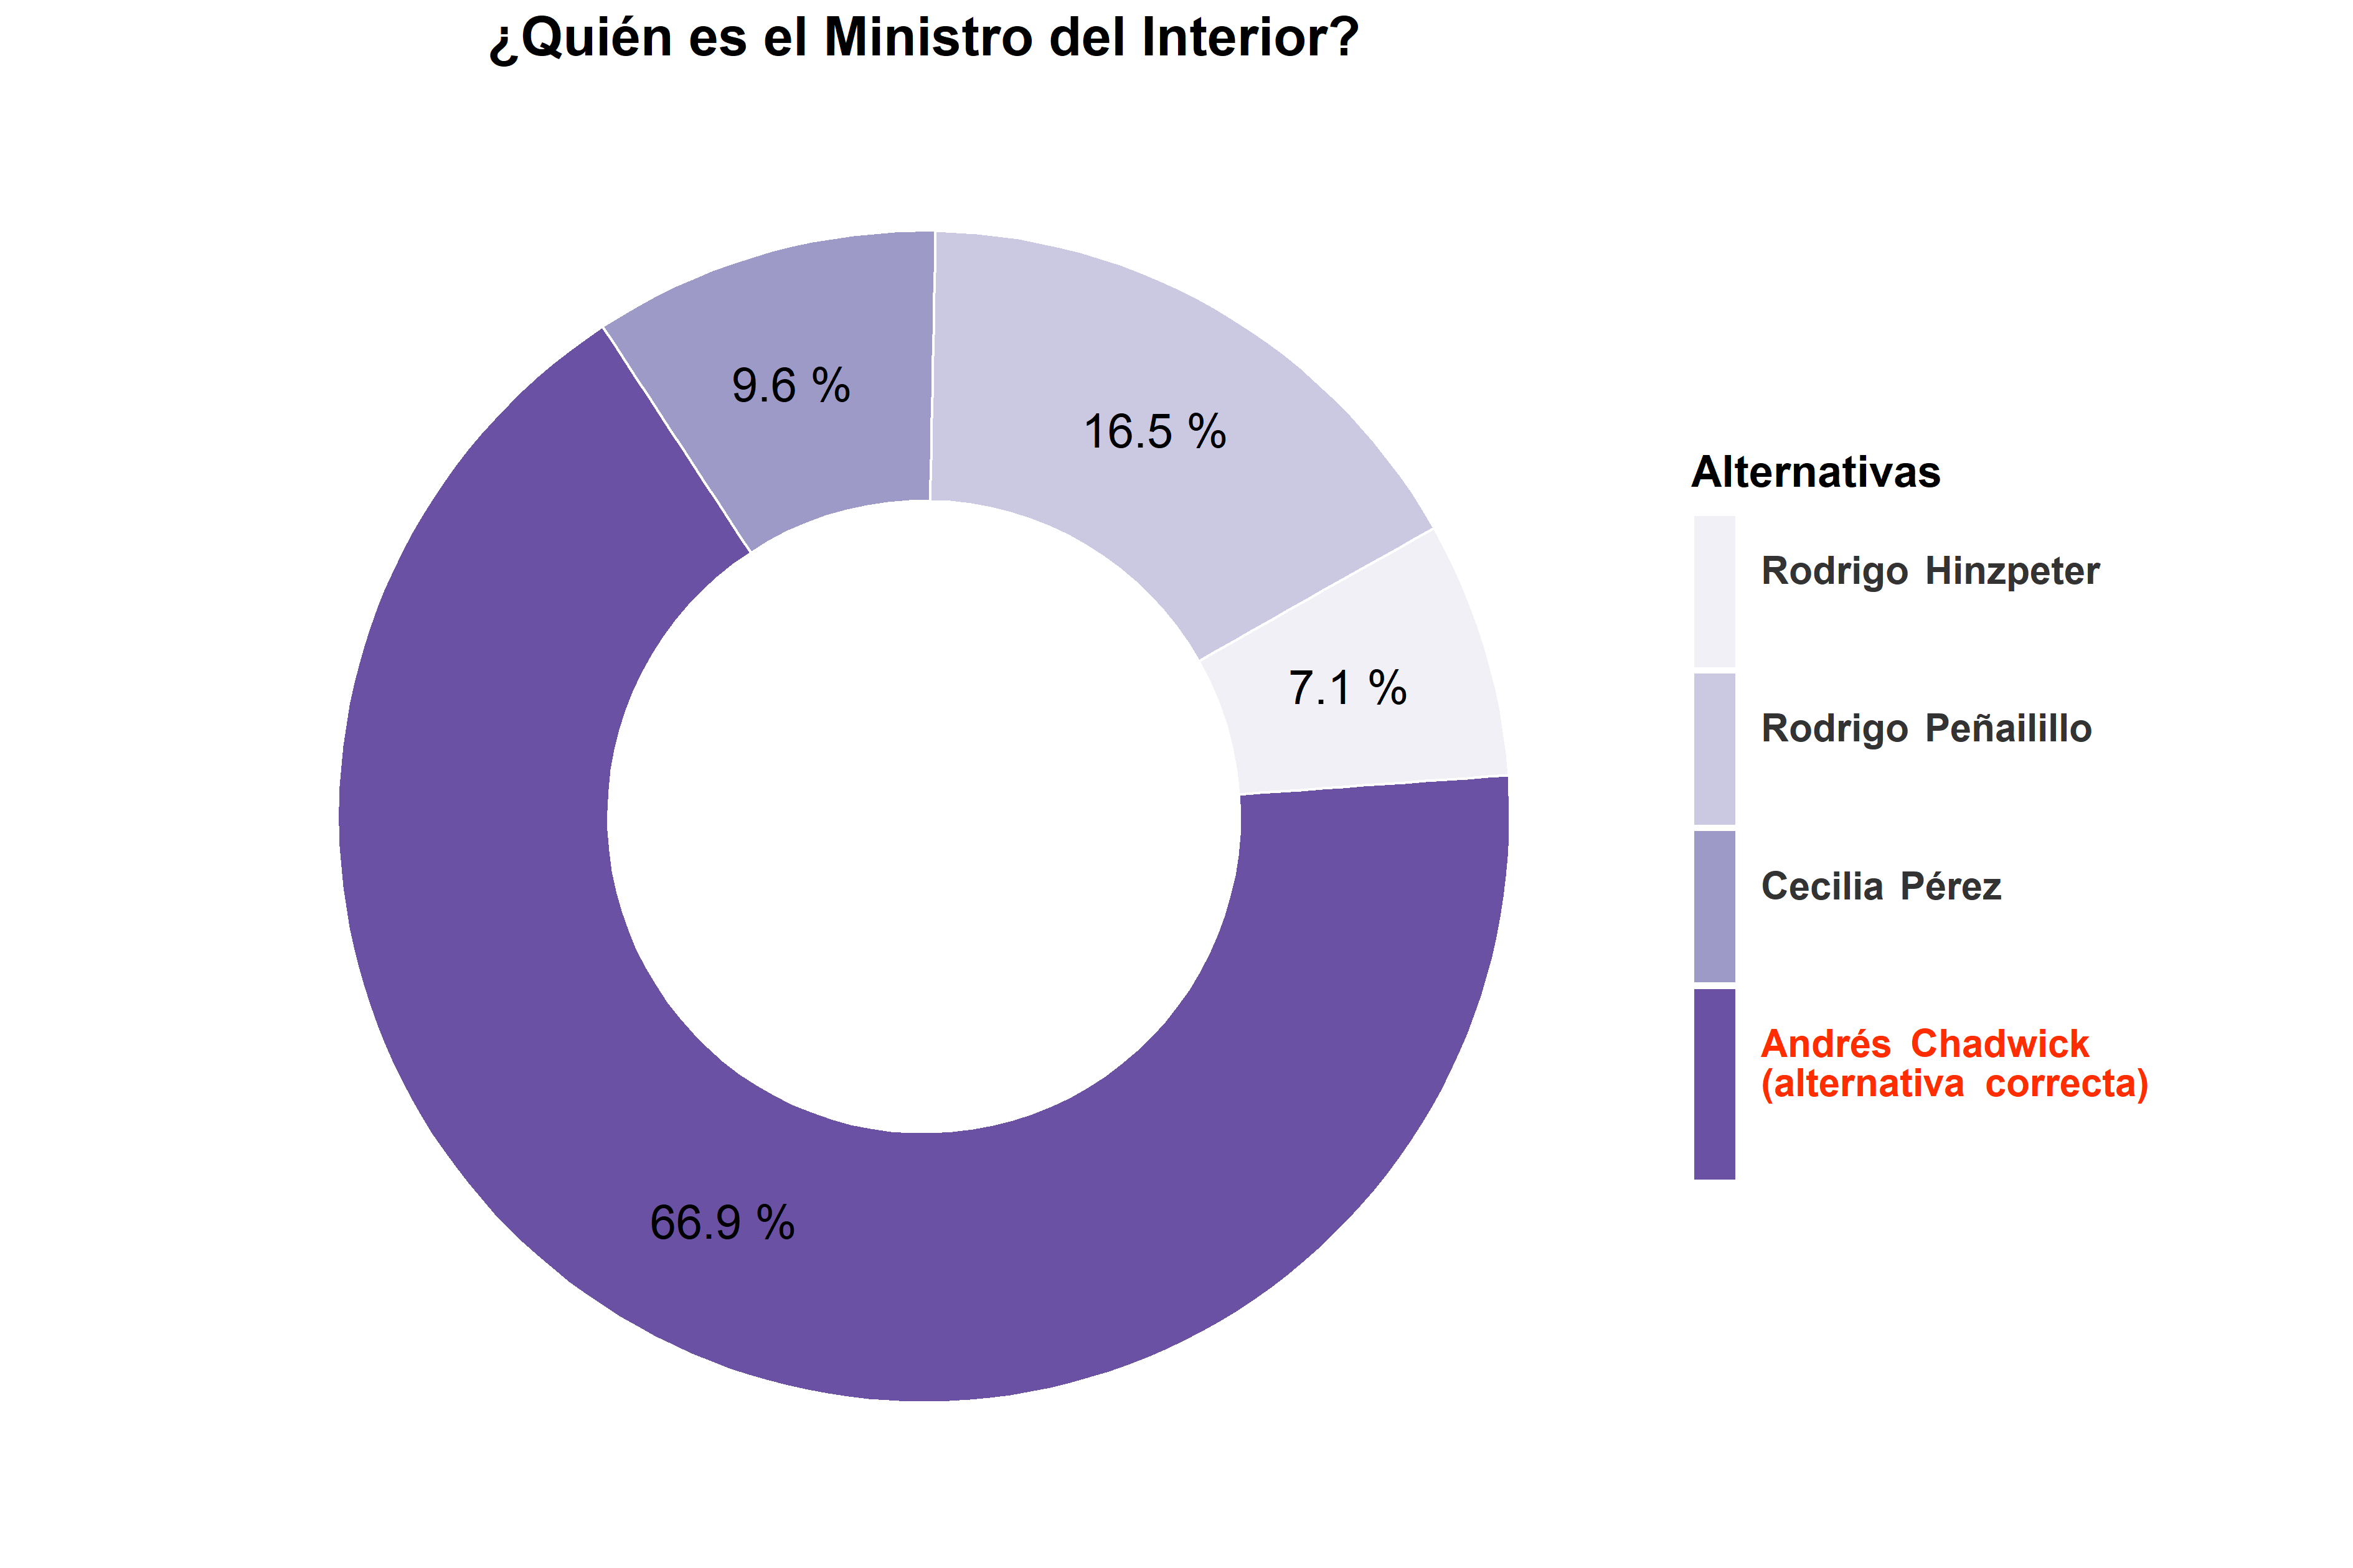
\includegraphics[width=52.49in]{images/ccivico_11} \end{center}

\hypertarget{duoduxe9cima-pregunta}{%
\subsubsection{Duodécima pregunta}\label{duoduxe9cima-pregunta}}

\begin{center}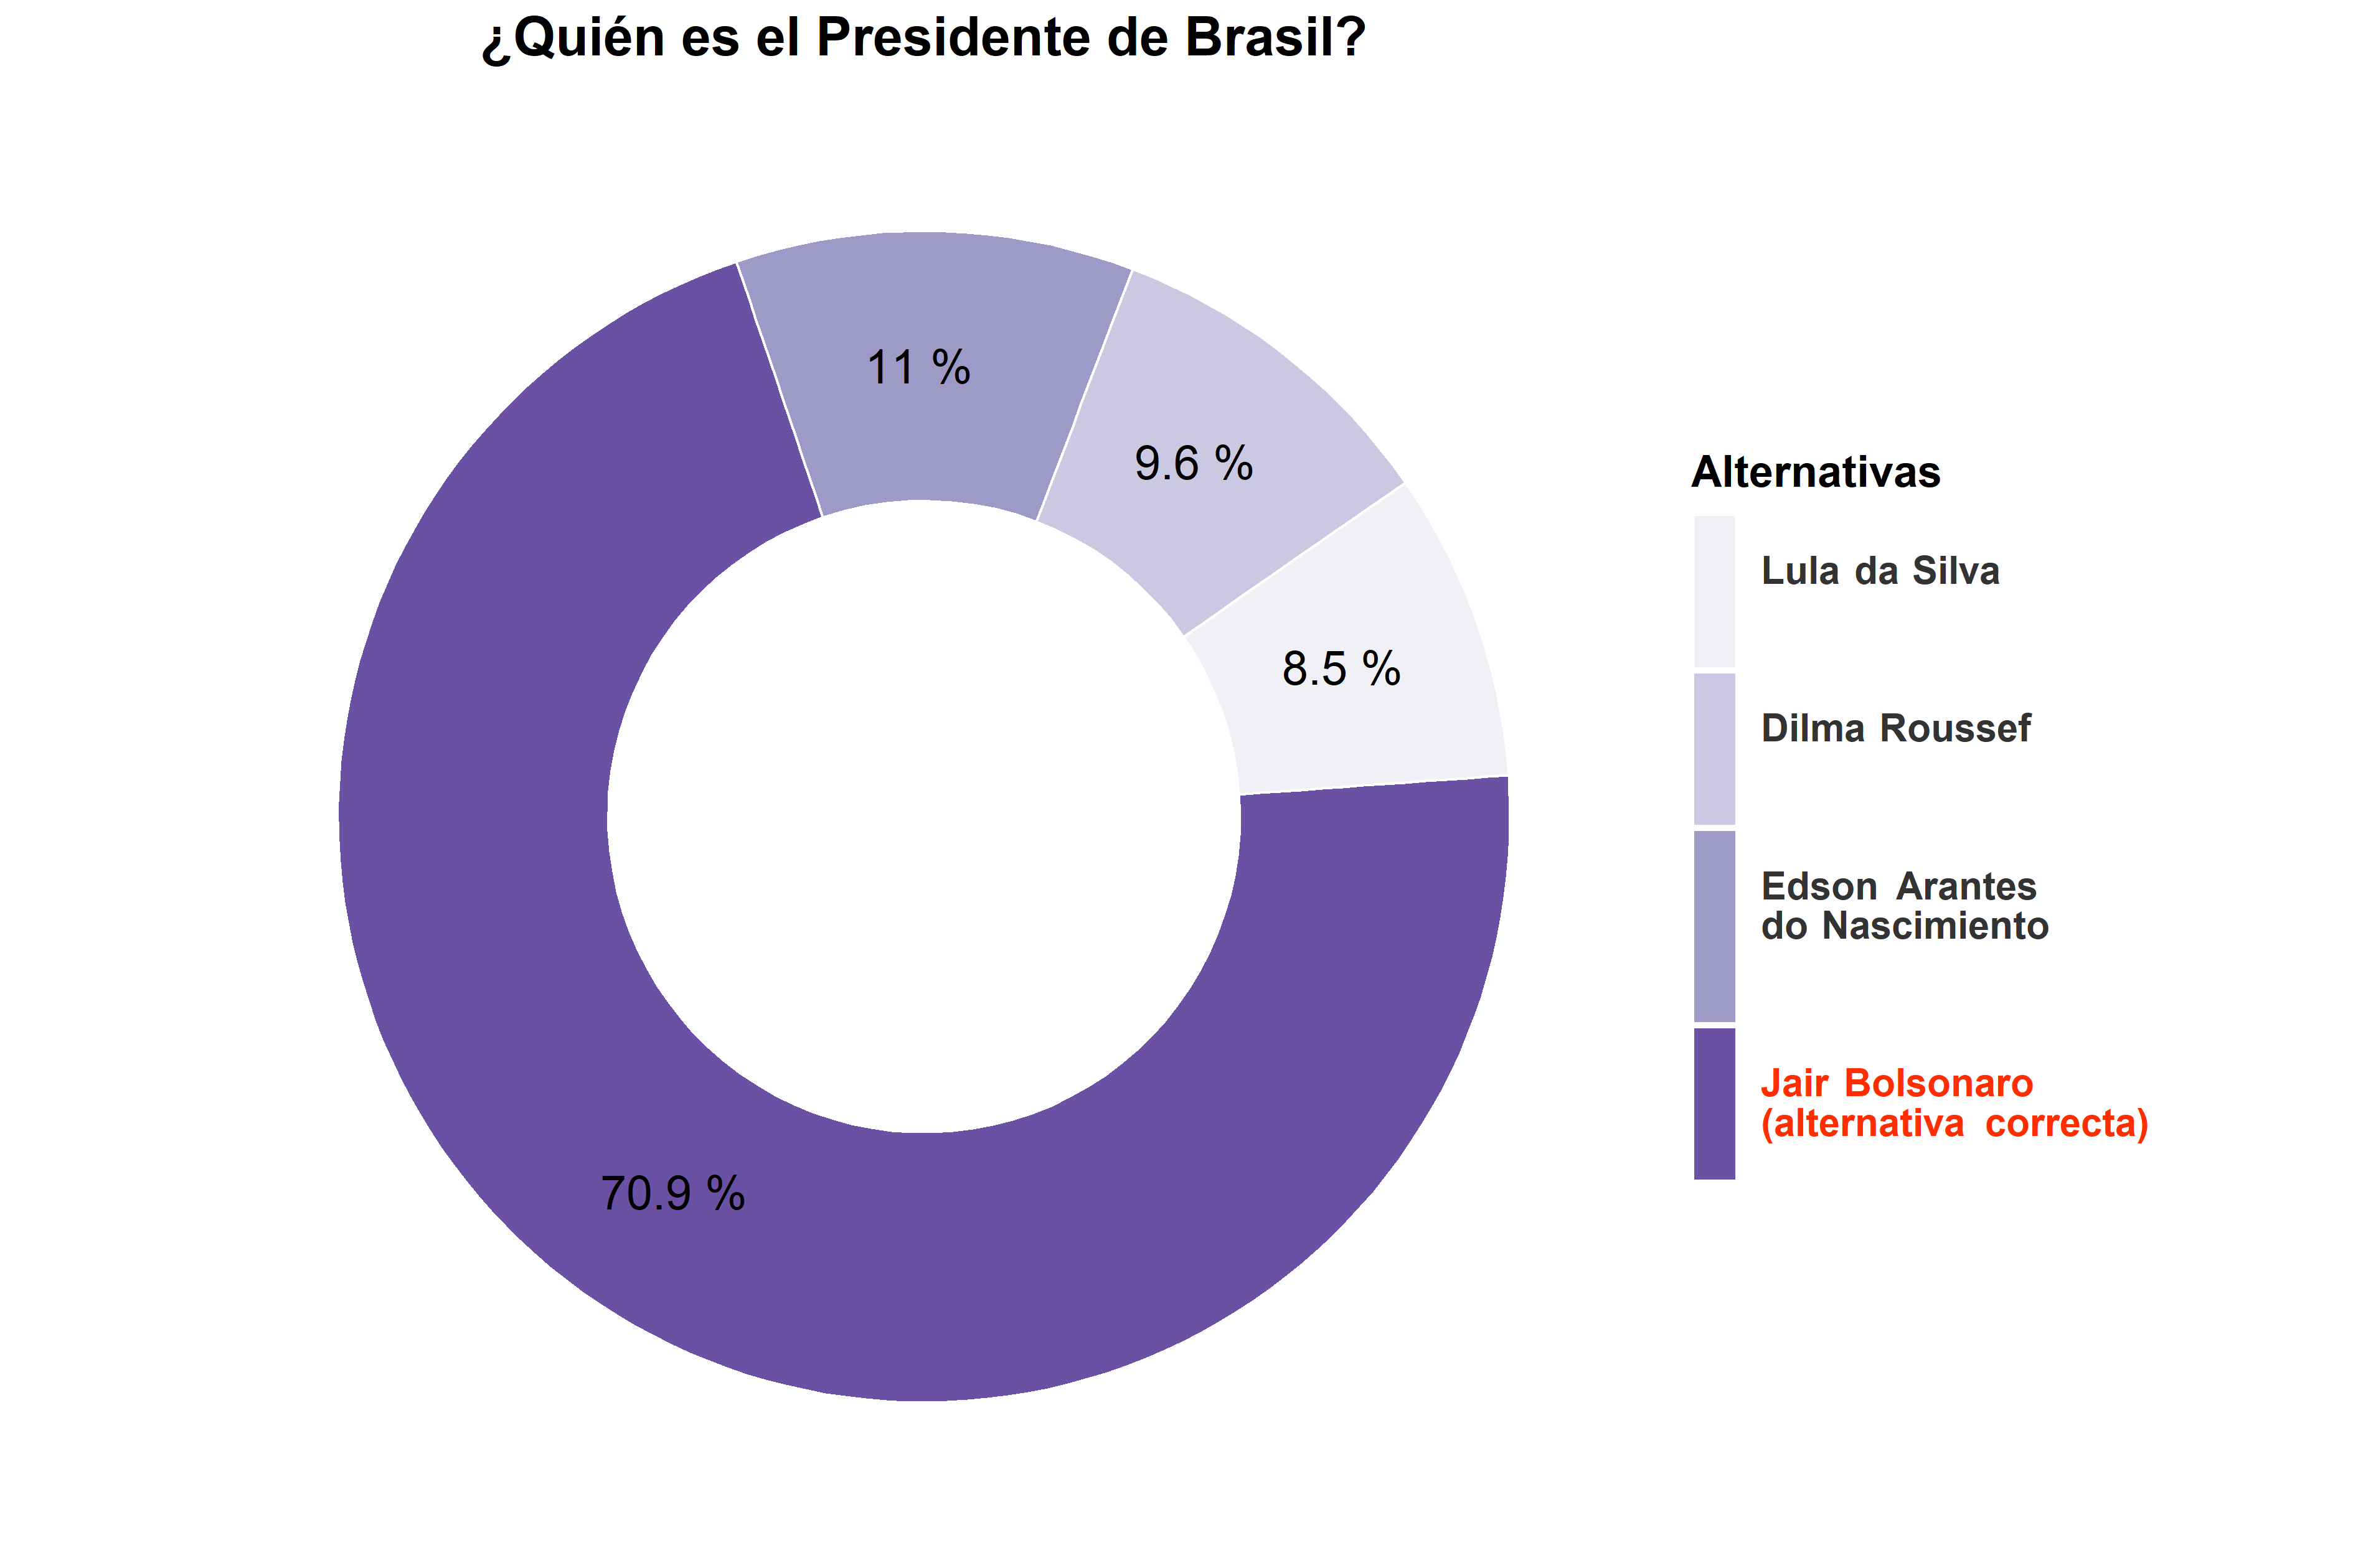
\includegraphics[width=52.49in]{images/ccivico_12} \end{center}

\hypertarget{decimotercera-pregunta}{%
\subsubsection{Decimotercera pregunta}\label{decimotercera-pregunta}}

\begin{center}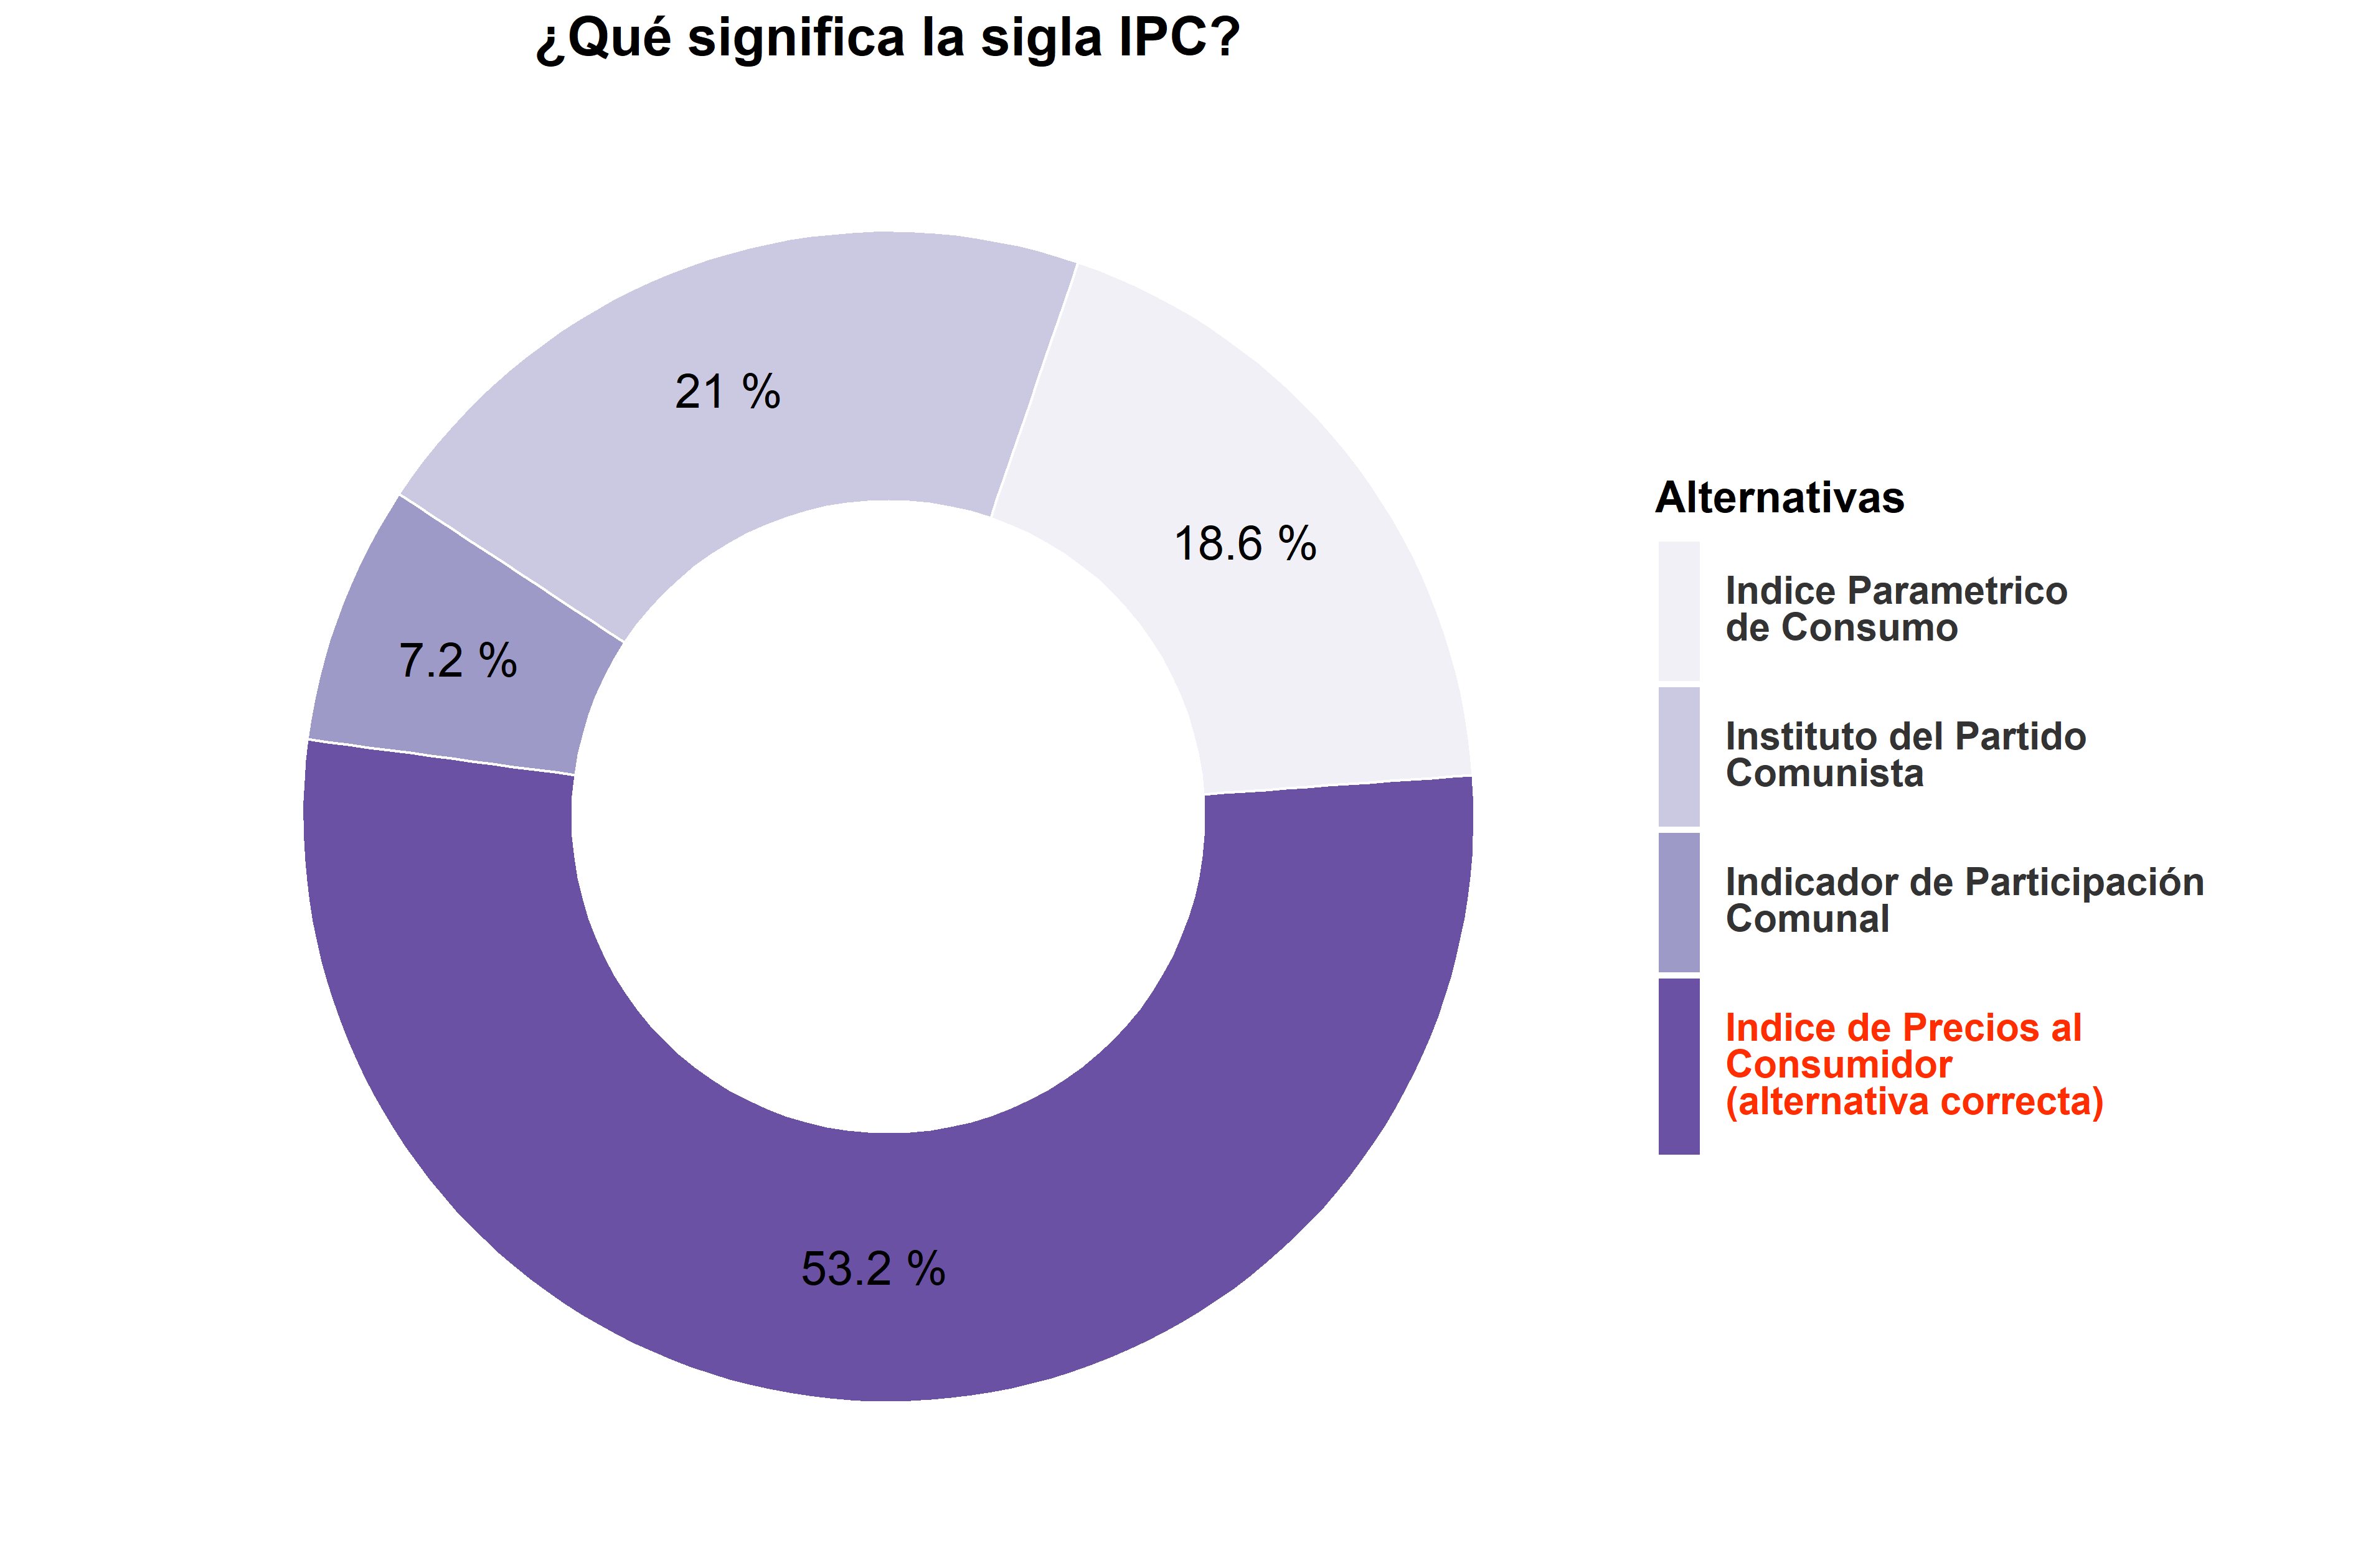
\includegraphics[width=52.49in]{images/ccivico_13} \end{center}

\hypertarget{decimocuarta-pregunta}{%
\subsubsection{Decimocuarta pregunta}\label{decimocuarta-pregunta}}

\begin{center}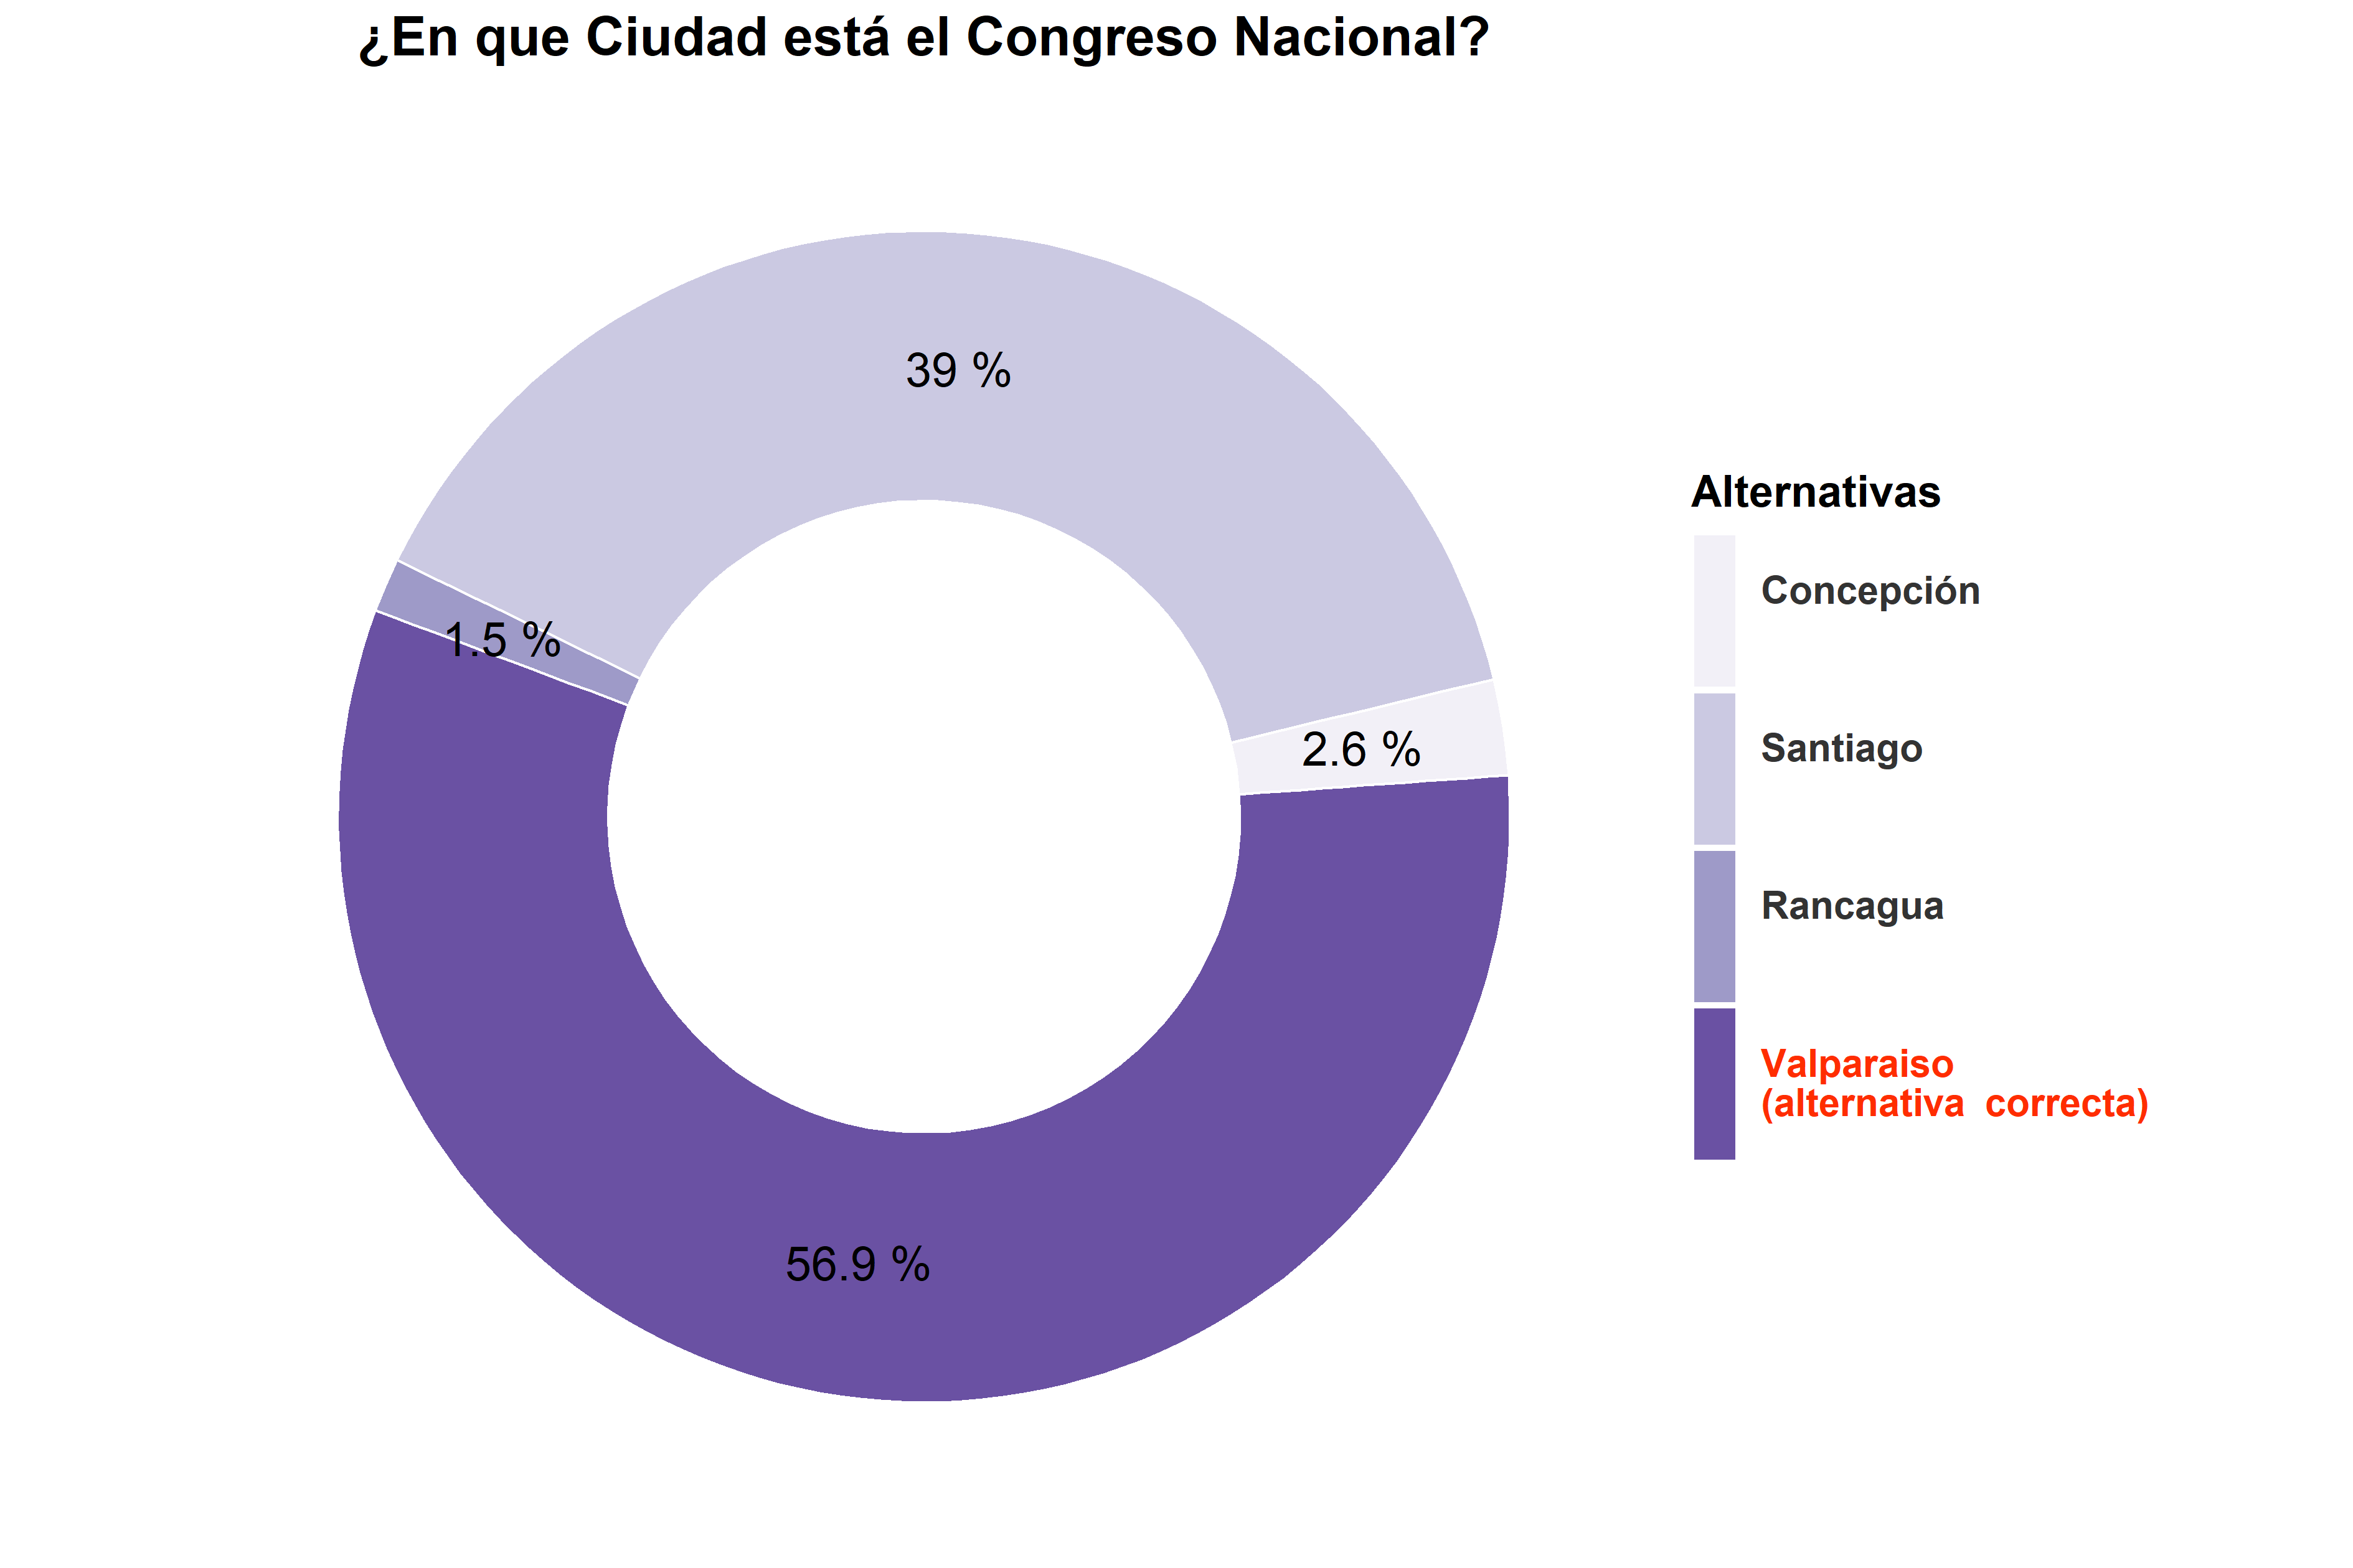
\includegraphics[width=52.49in]{images/ccivico_14} \end{center}

\hypertarget{comparaciuxf3n-con-el-estudio-iccs-2009}{%
\subsection{Comparación con el estudio ICCS 2009}\label{comparaciuxf3n-con-el-estudio-iccs-2009}}

\hypertarget{primera-pregunta}{%
\subsubsection{Primera pregunta}\label{primera-pregunta}}

\begin{center}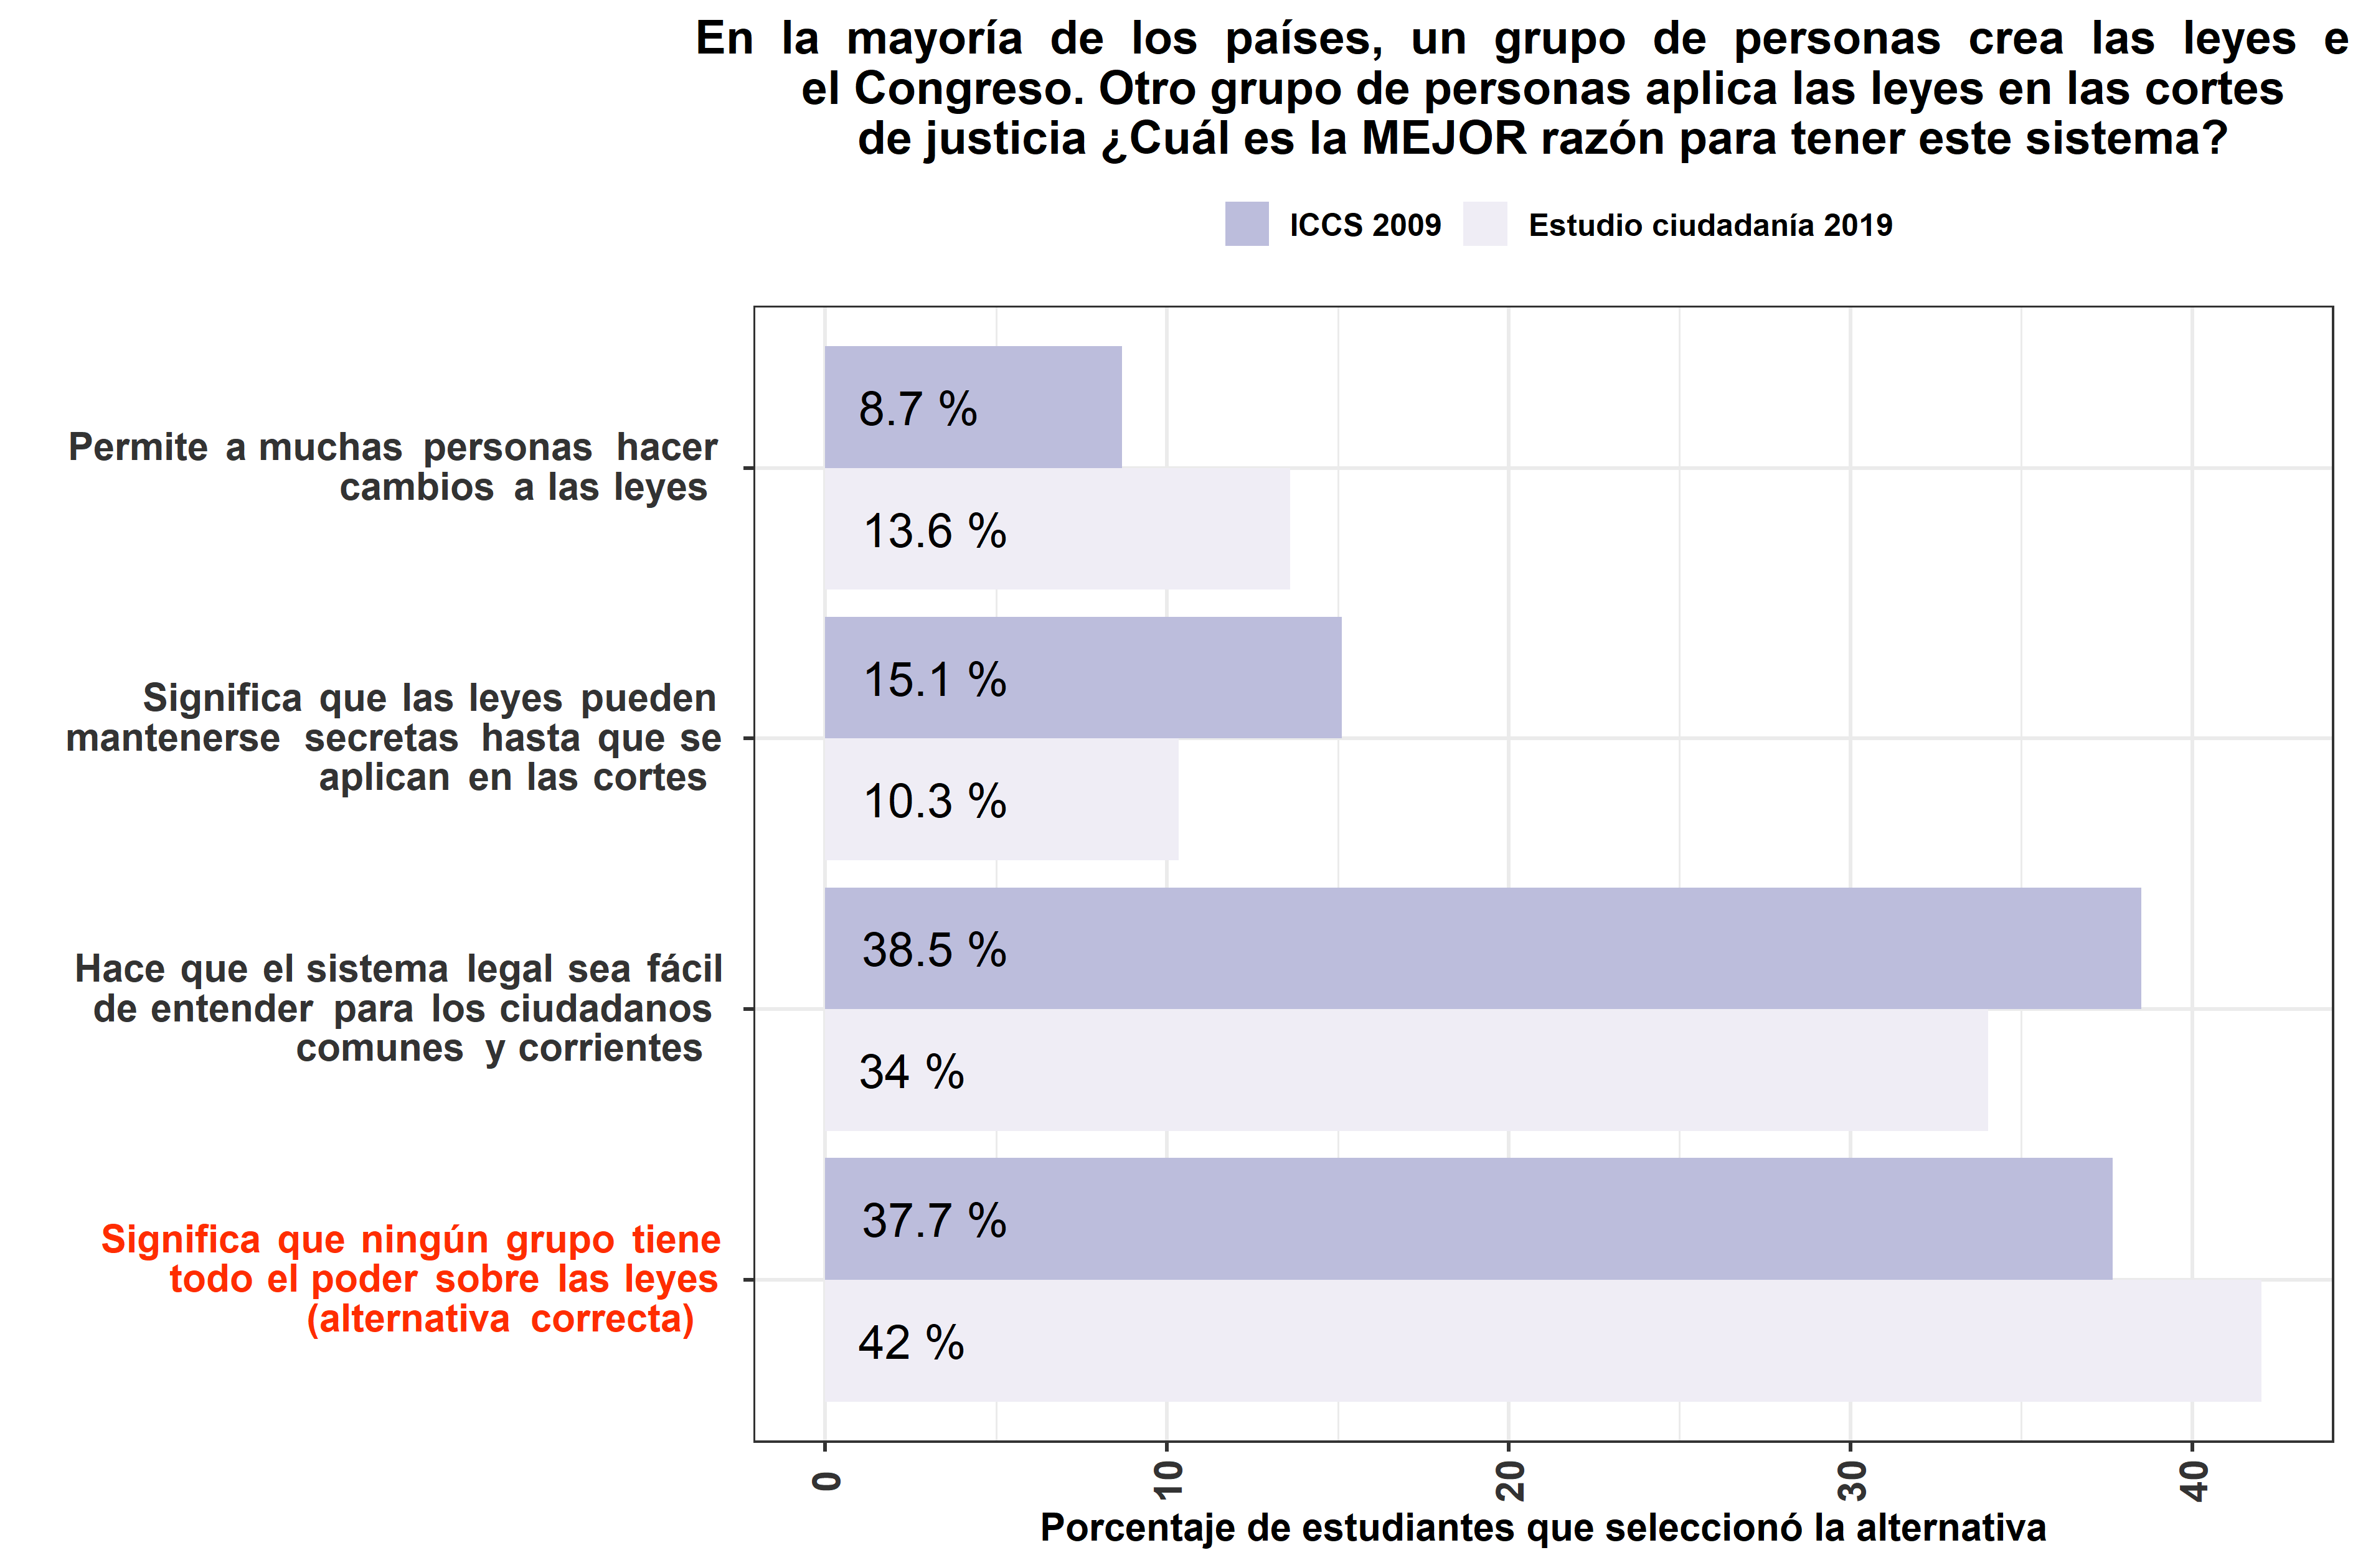
\includegraphics[width=52.49in]{images/graph_p1} \end{center}

\hypertarget{segunda-pregunta-1}{%
\subsubsection{Segunda pregunta}\label{segunda-pregunta-1}}

\begin{center}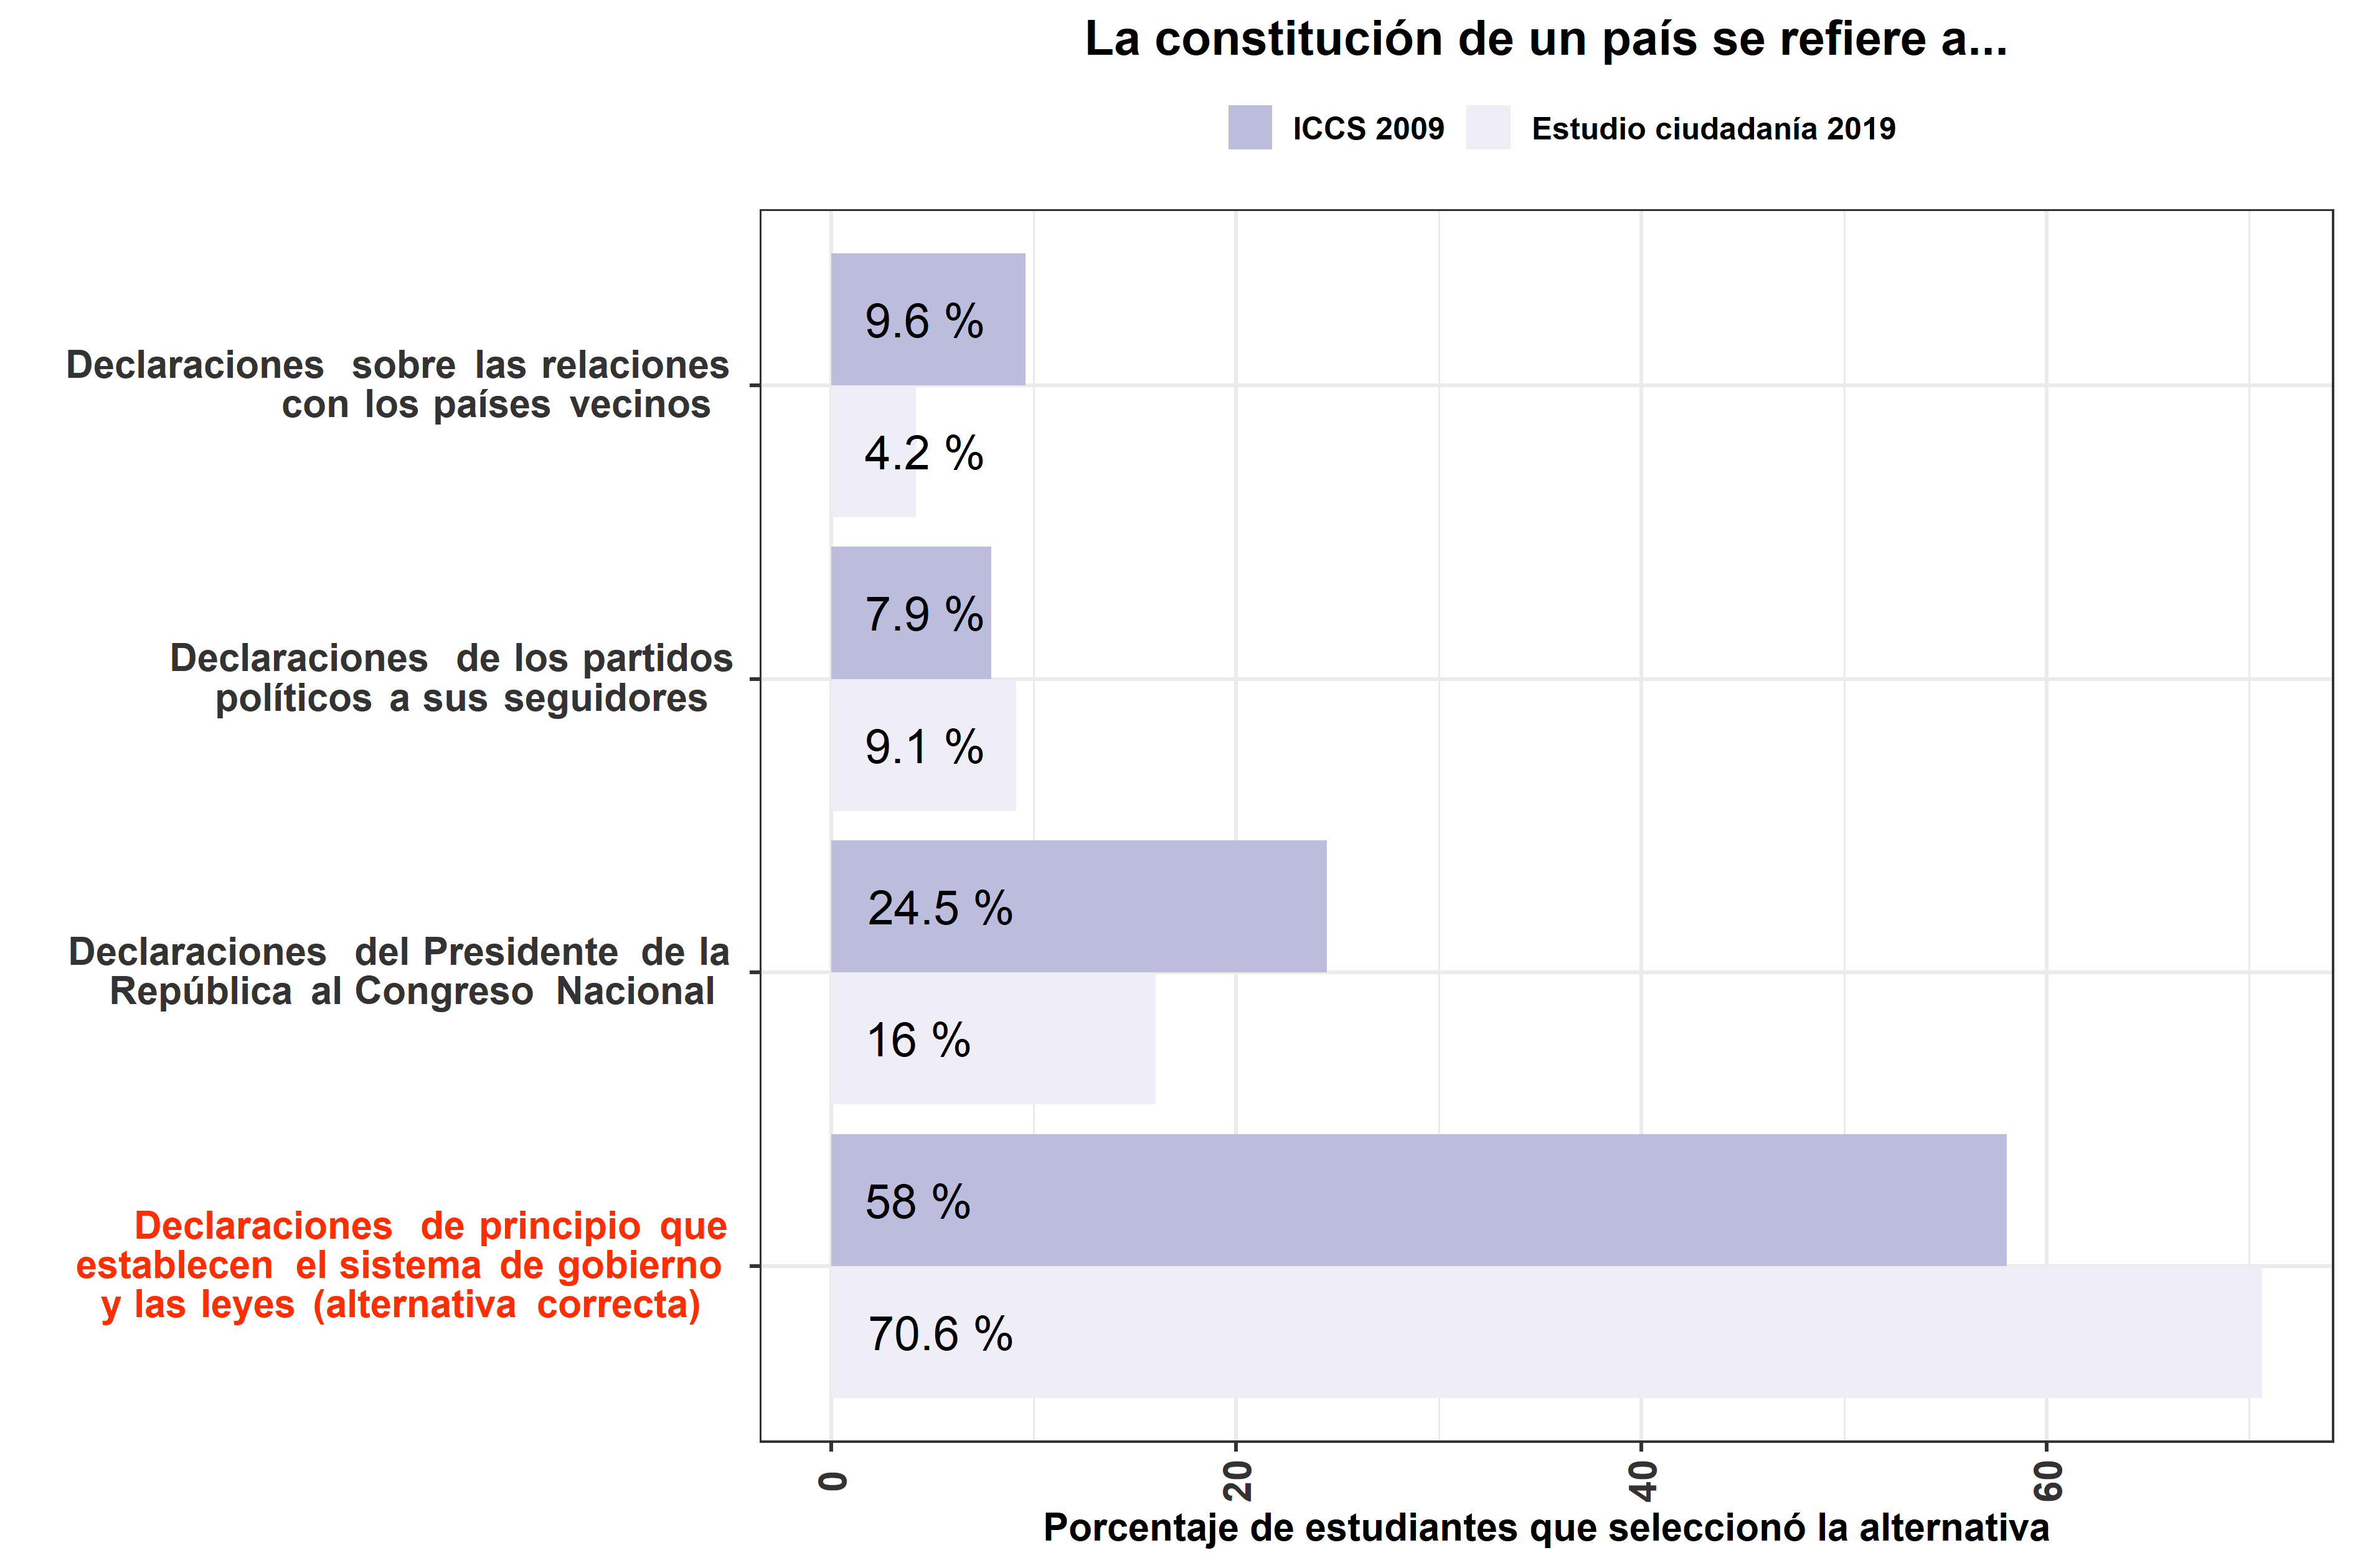
\includegraphics[width=52.49in]{images/graph_p2} \end{center}

\hypertarget{tercera-pregunta-1}{%
\subsubsection{Tercera pregunta}\label{tercera-pregunta-1}}

\begin{center}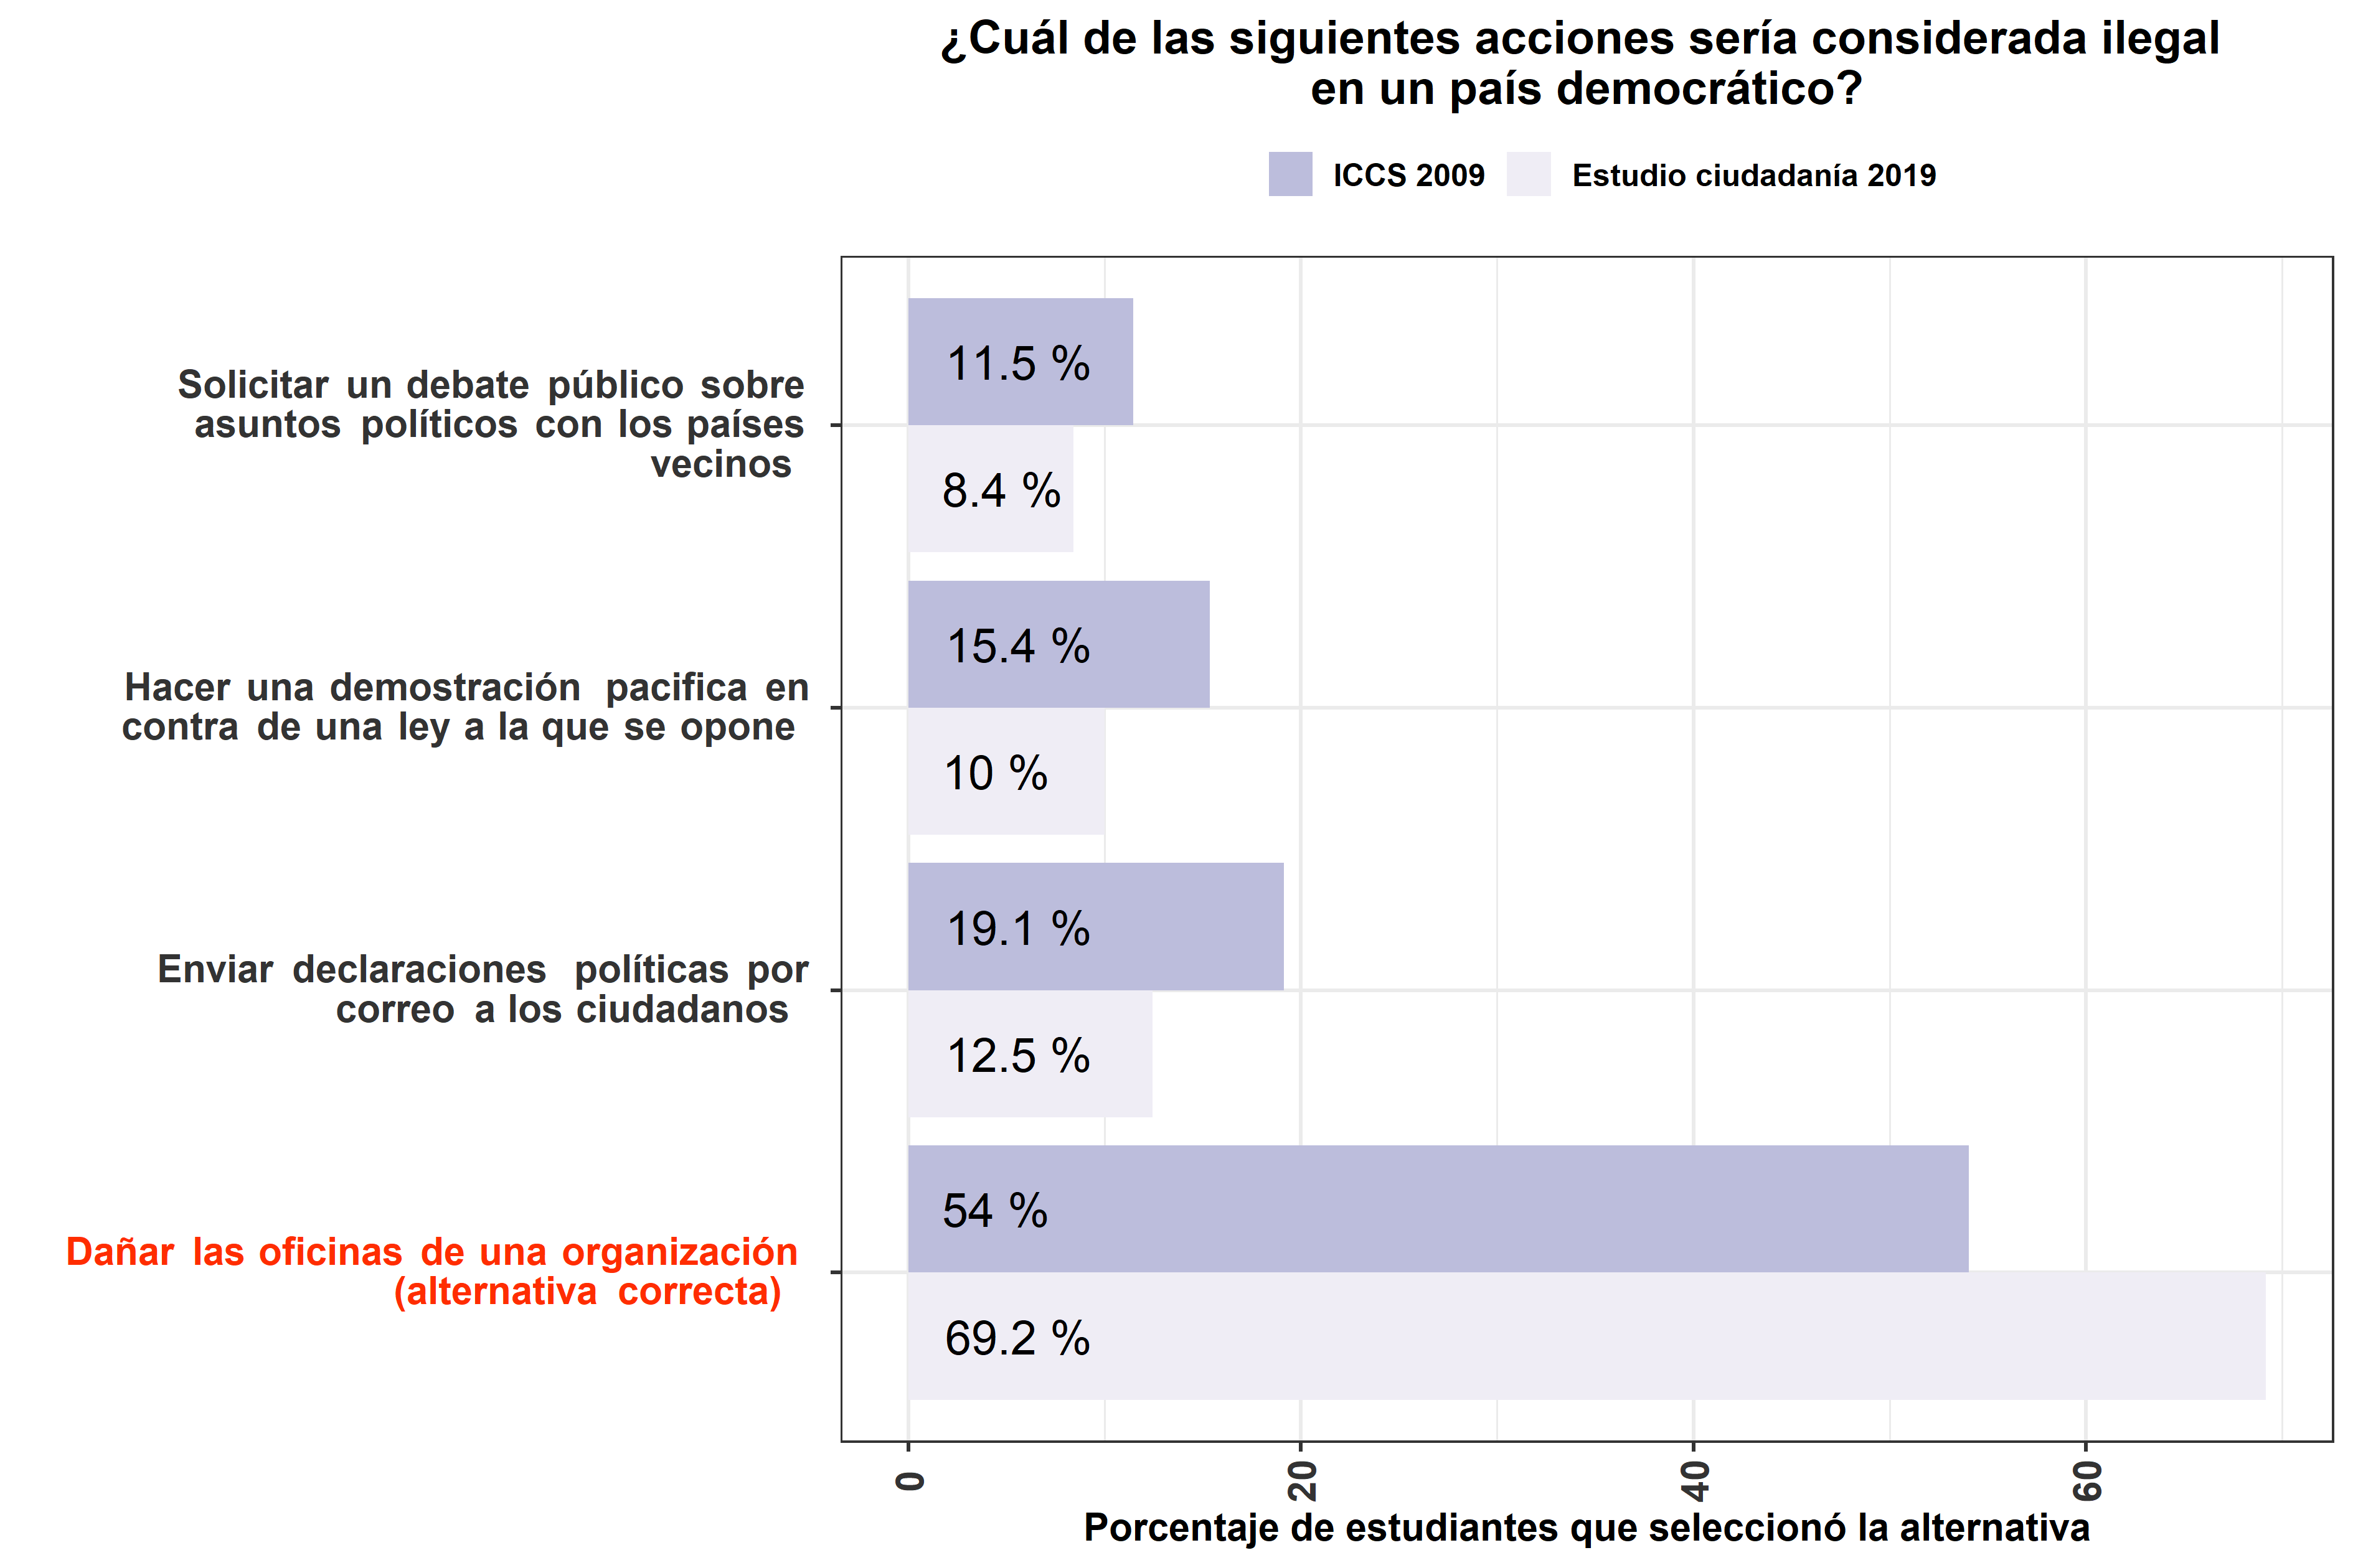
\includegraphics[width=52.49in]{images/graph_p3} \end{center}

\hypertarget{cuarta-pregunta-1}{%
\subsubsection{Cuarta pregunta}\label{cuarta-pregunta-1}}

\begin{center}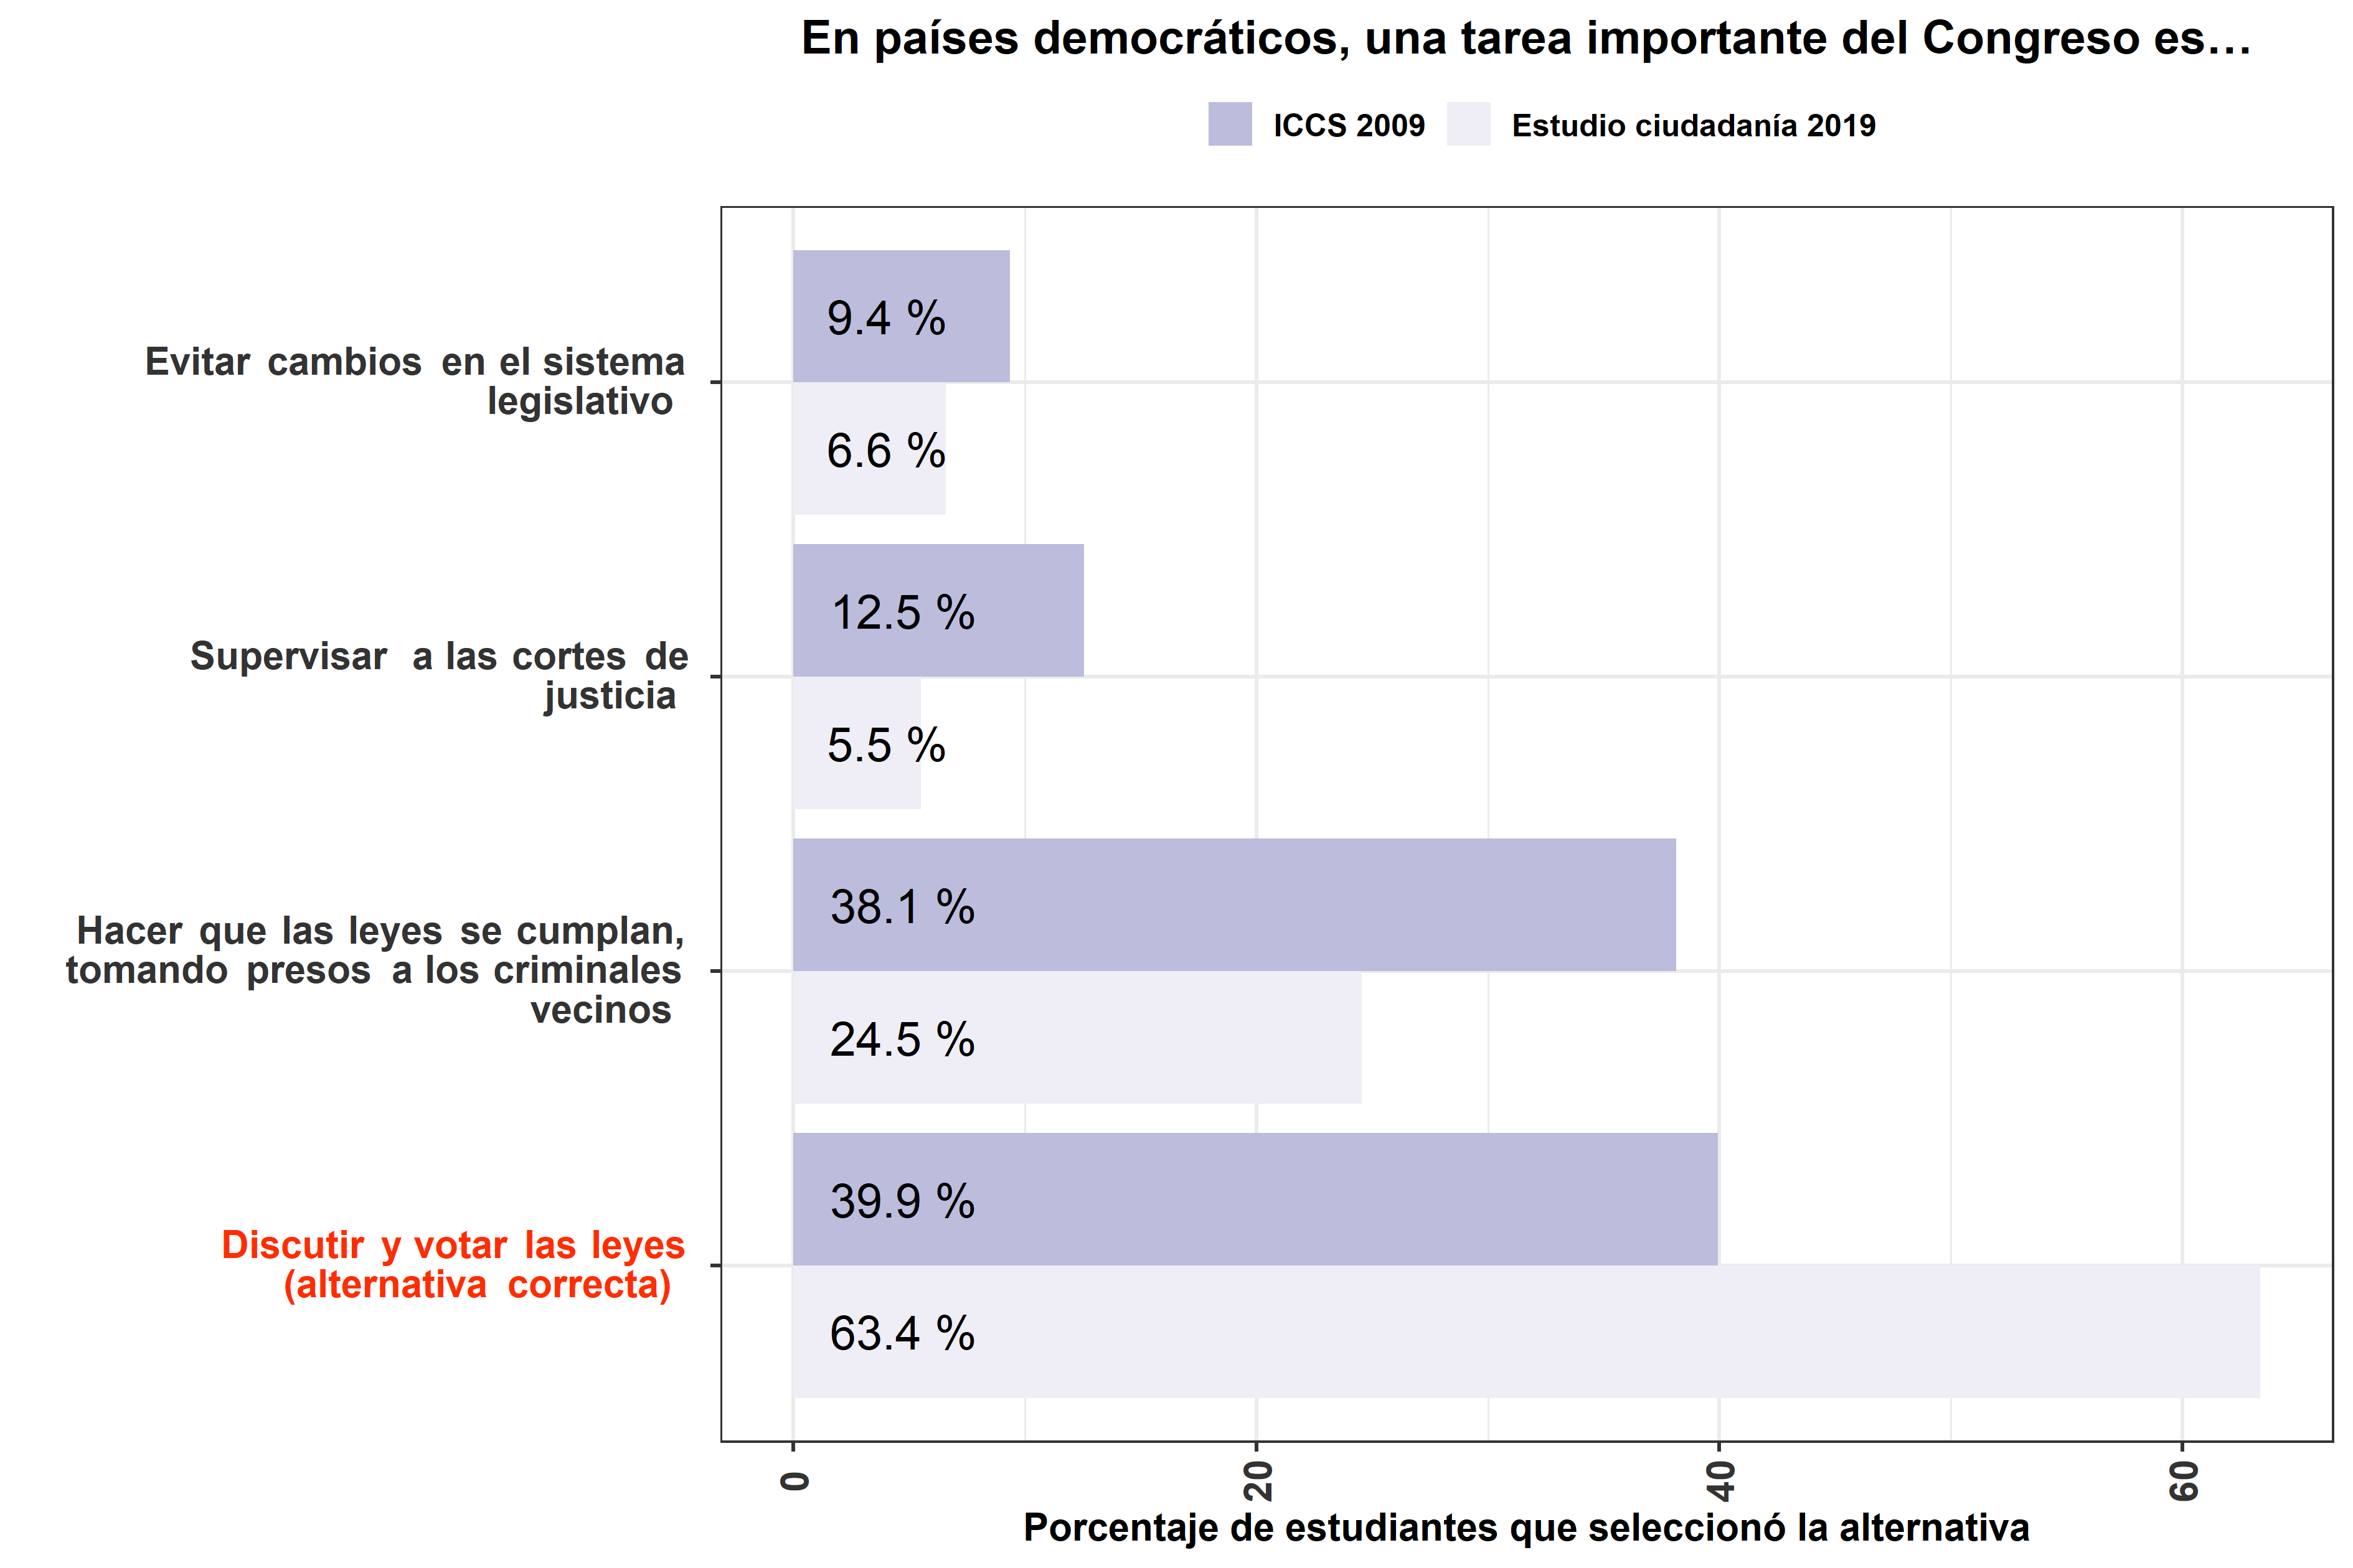
\includegraphics[width=52.49in]{images/graph_p4} \end{center}

\hypertarget{quinta-pregunta-1}{%
\subsubsection{Quinta pregunta}\label{quinta-pregunta-1}}

\begin{center}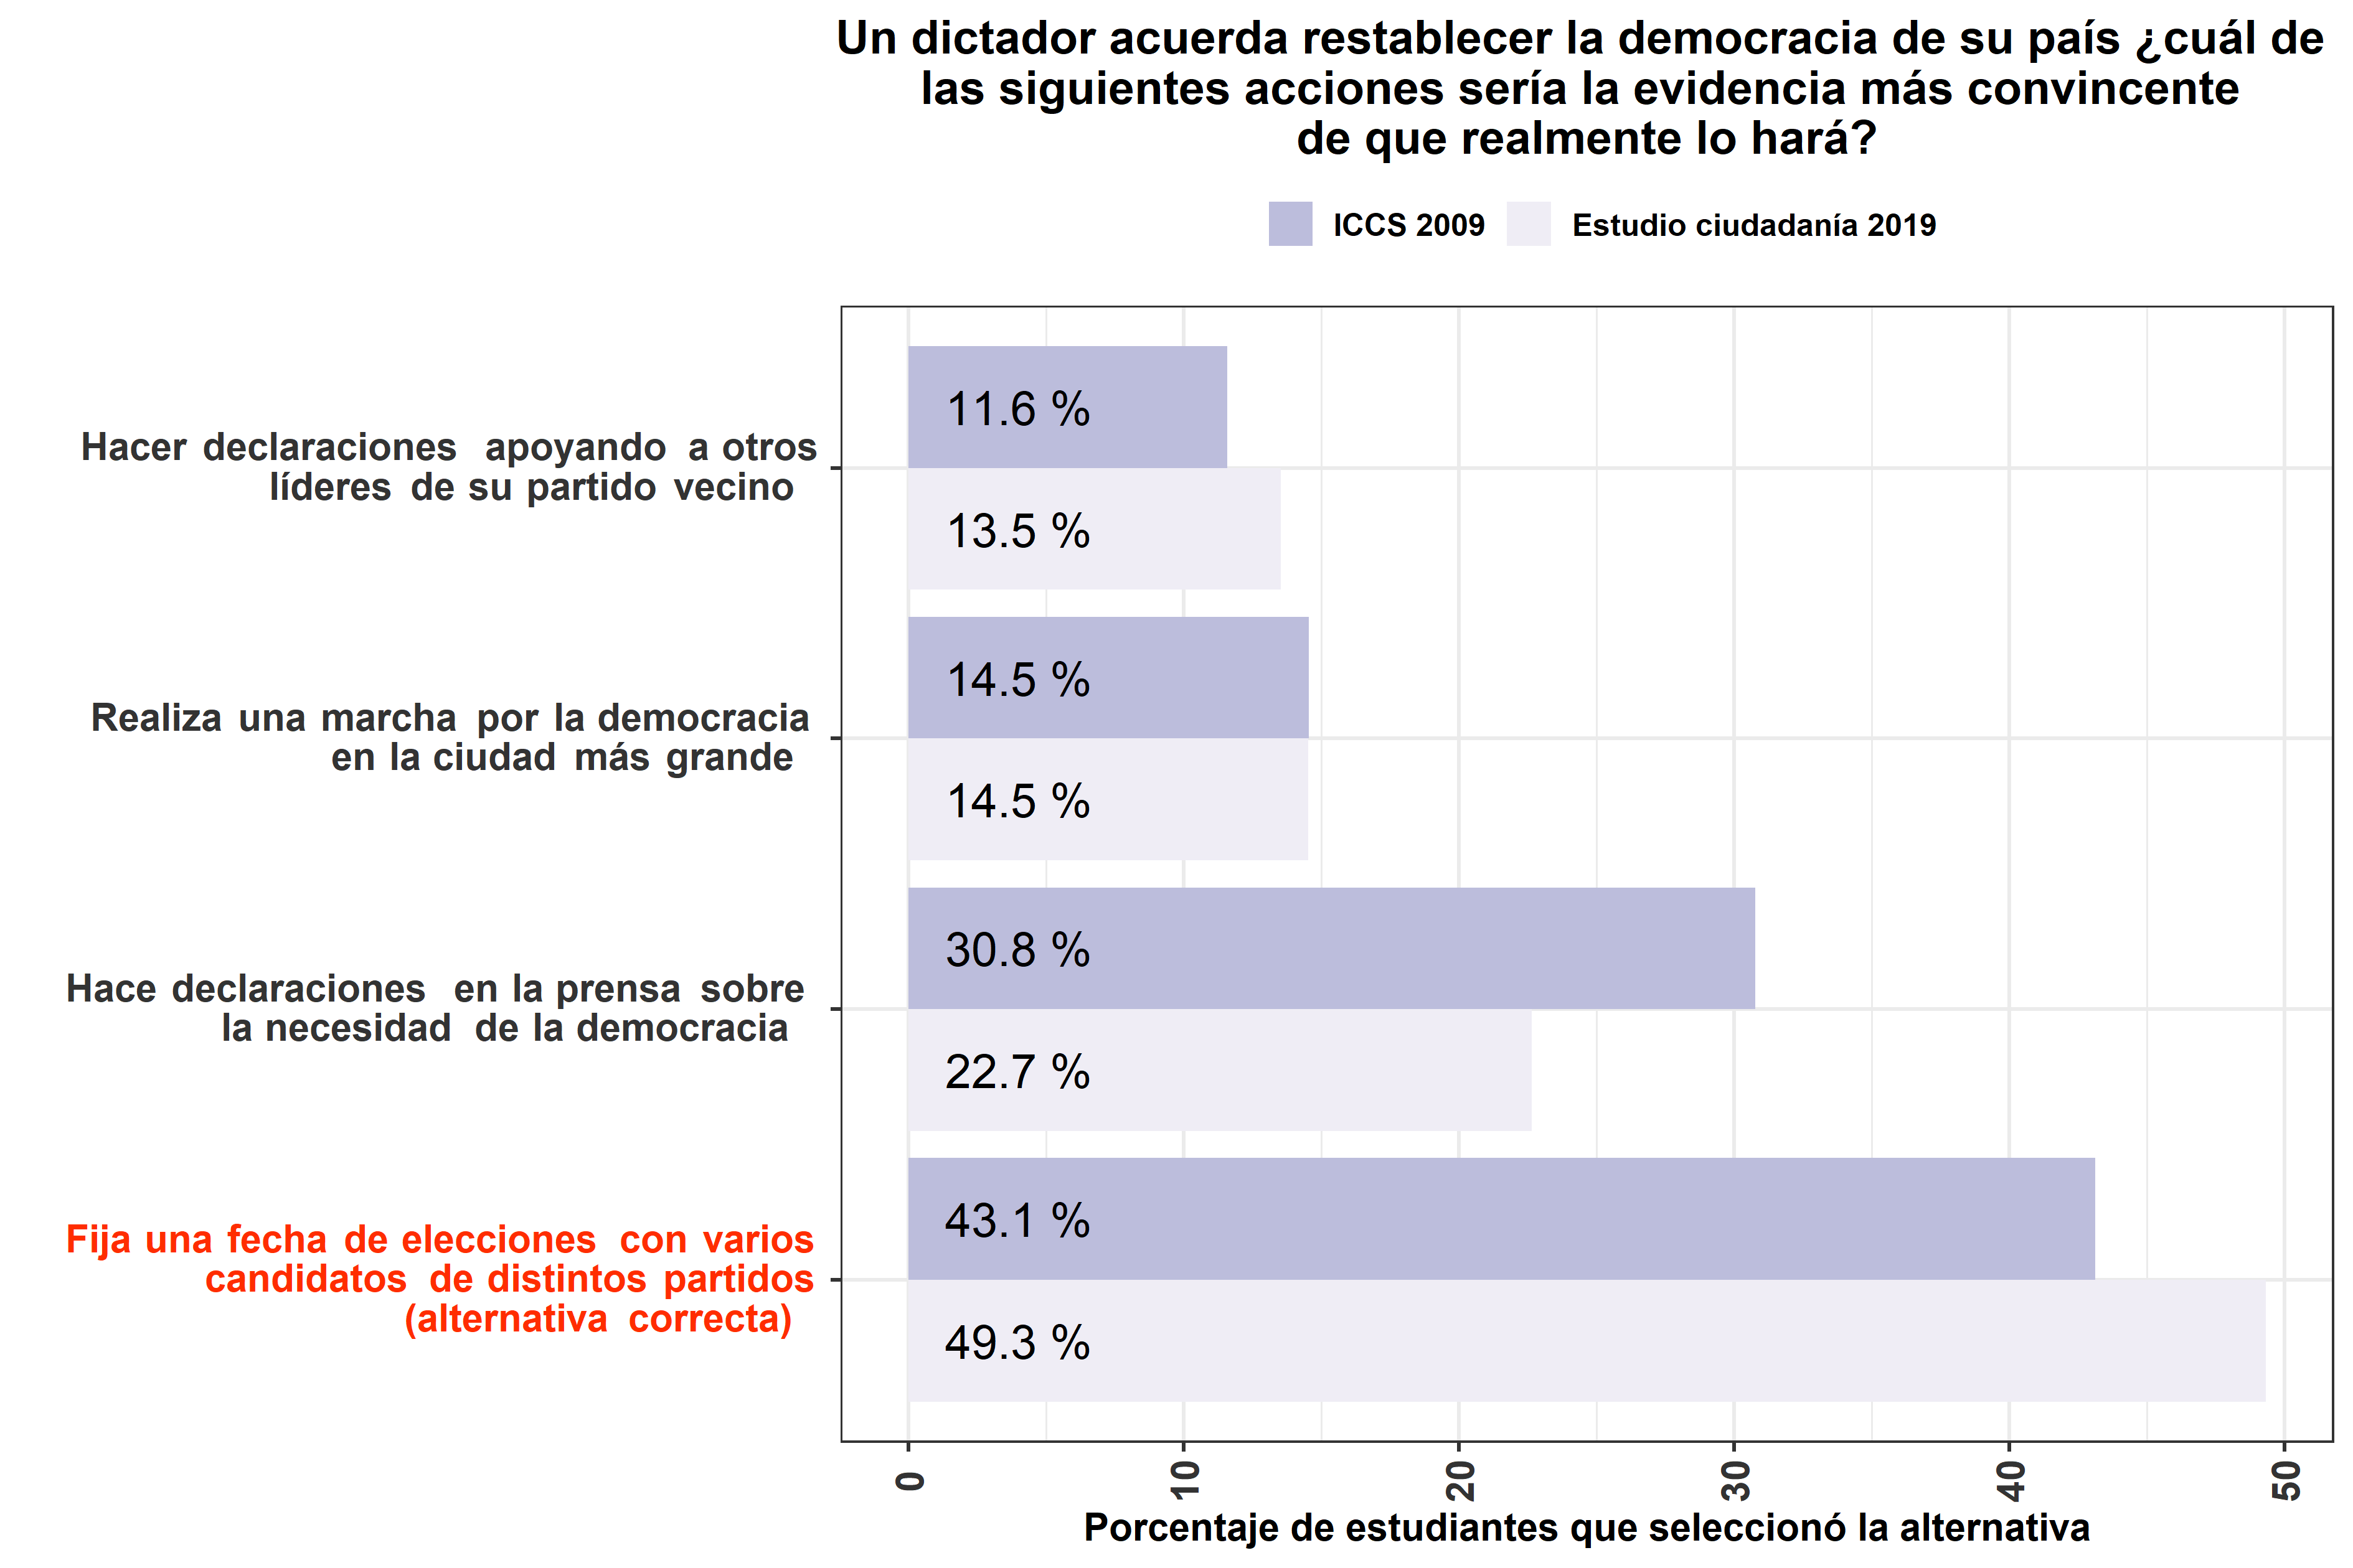
\includegraphics[width=52.49in]{images/graph_p5} \end{center}

\hypertarget{sexta-pregunta-1}{%
\subsubsection{Sexta pregunta}\label{sexta-pregunta-1}}

\begin{center}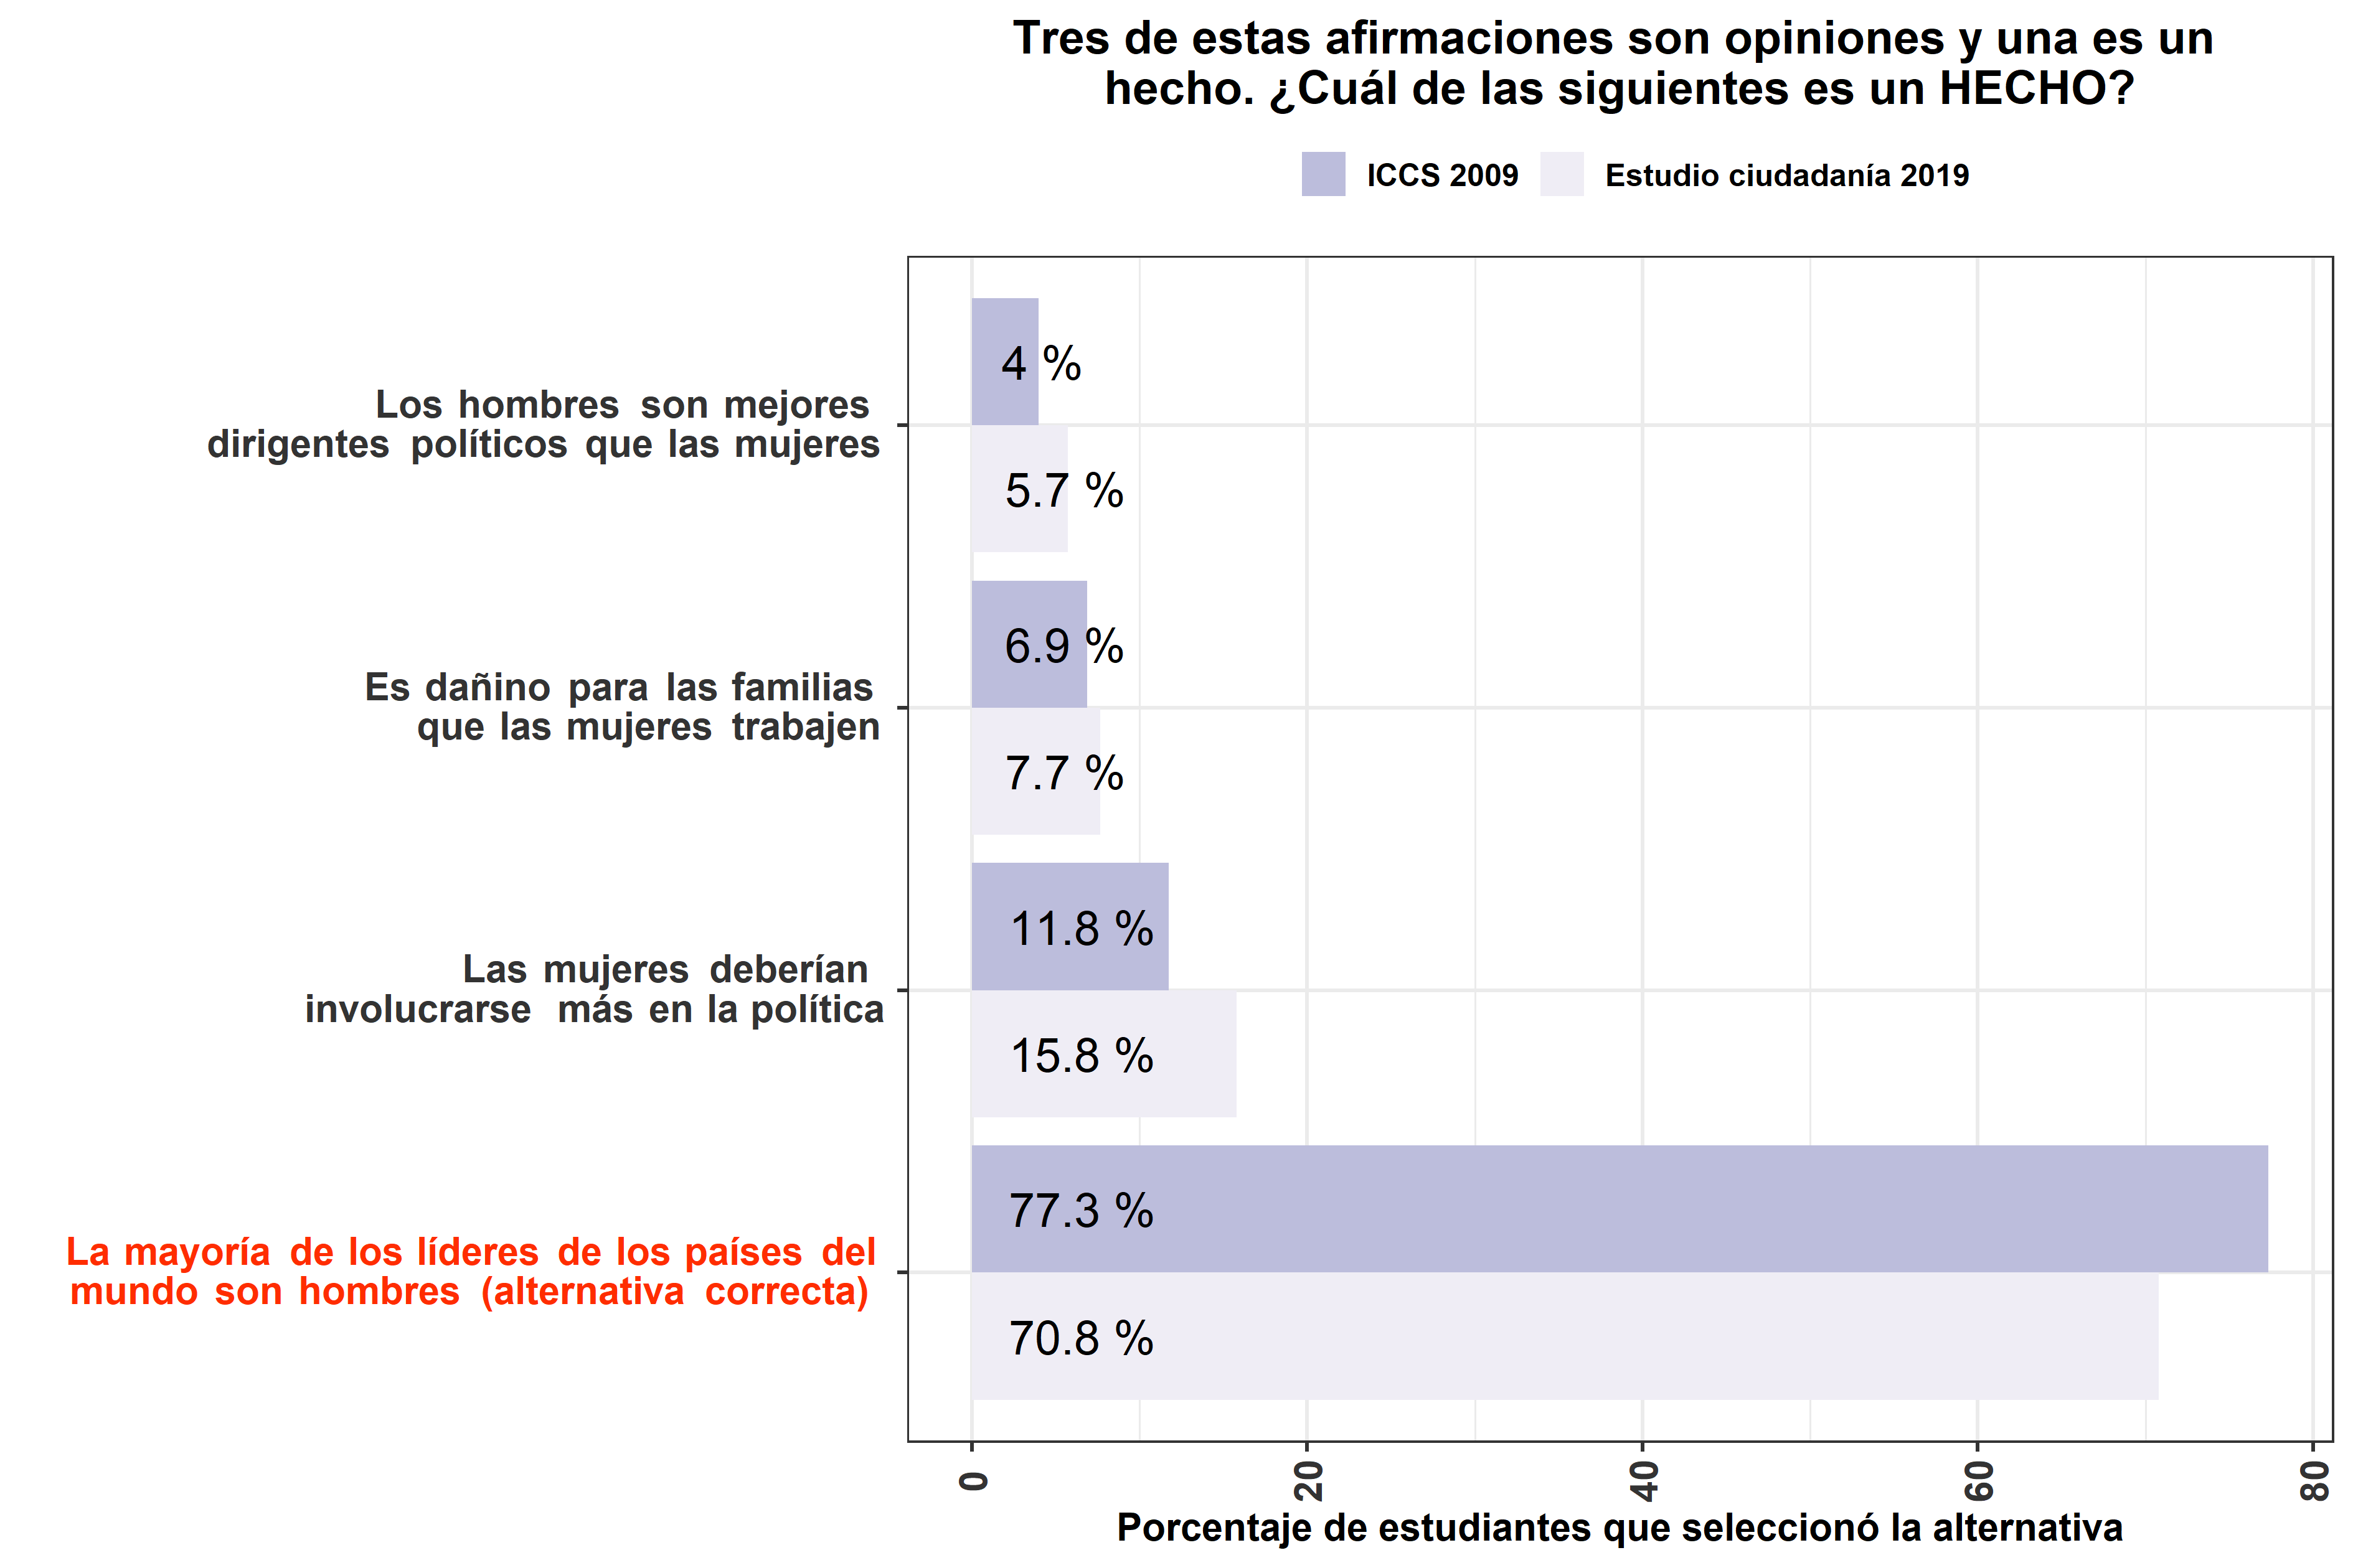
\includegraphics[width=52.49in]{images/graph_p6} \end{center}

\hypertarget{secciuxf3n-2-clima-democruxe1tico-en-el-aula}{%
\section{Sección 2: Clima democrático en el aula}\label{secciuxf3n-2-clima-democruxe1tico-en-el-aula}}

\hypertarget{importancia-de-distintos-aspectos-en-la-formaciuxf3n-ciudadana}{%
\subsection{Importancia de distintos aspectos en la formación ciudadana}\label{importancia-de-distintos-aspectos-en-la-formaciuxf3n-ciudadana}}

\begin{center}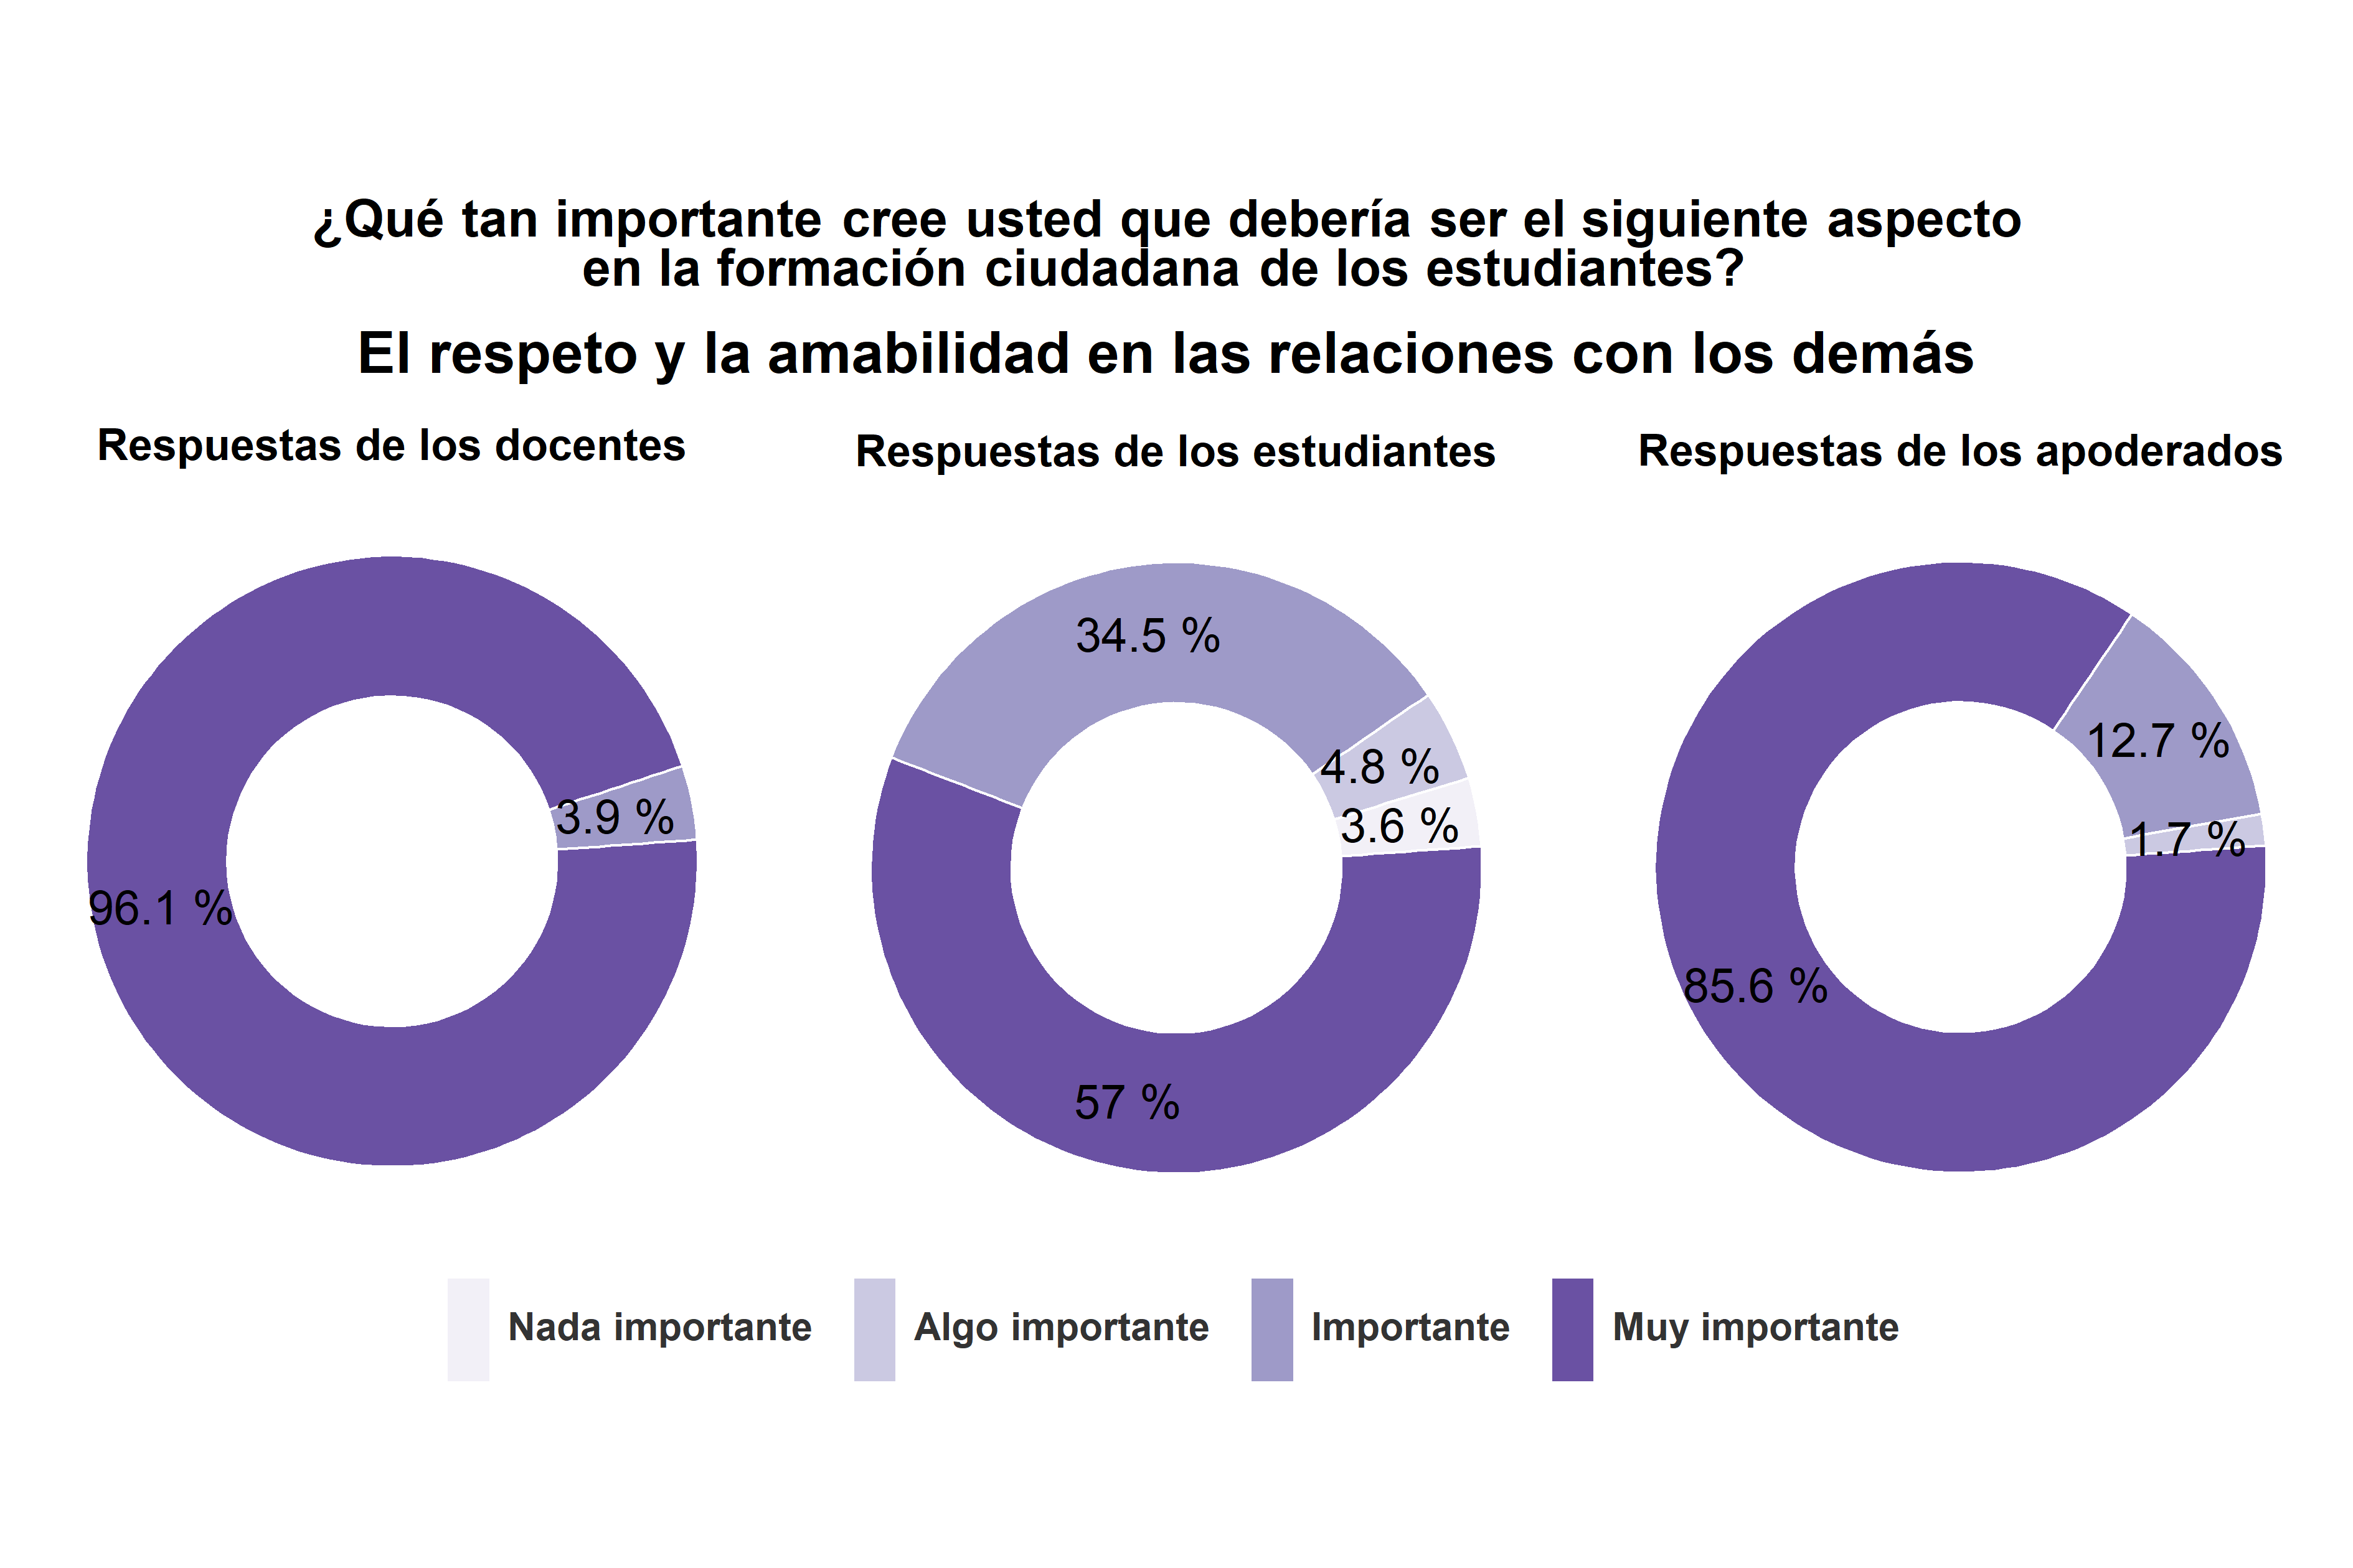
\includegraphics[width=52.49in]{images/graph_for_ciud1} \end{center}

\begin{center}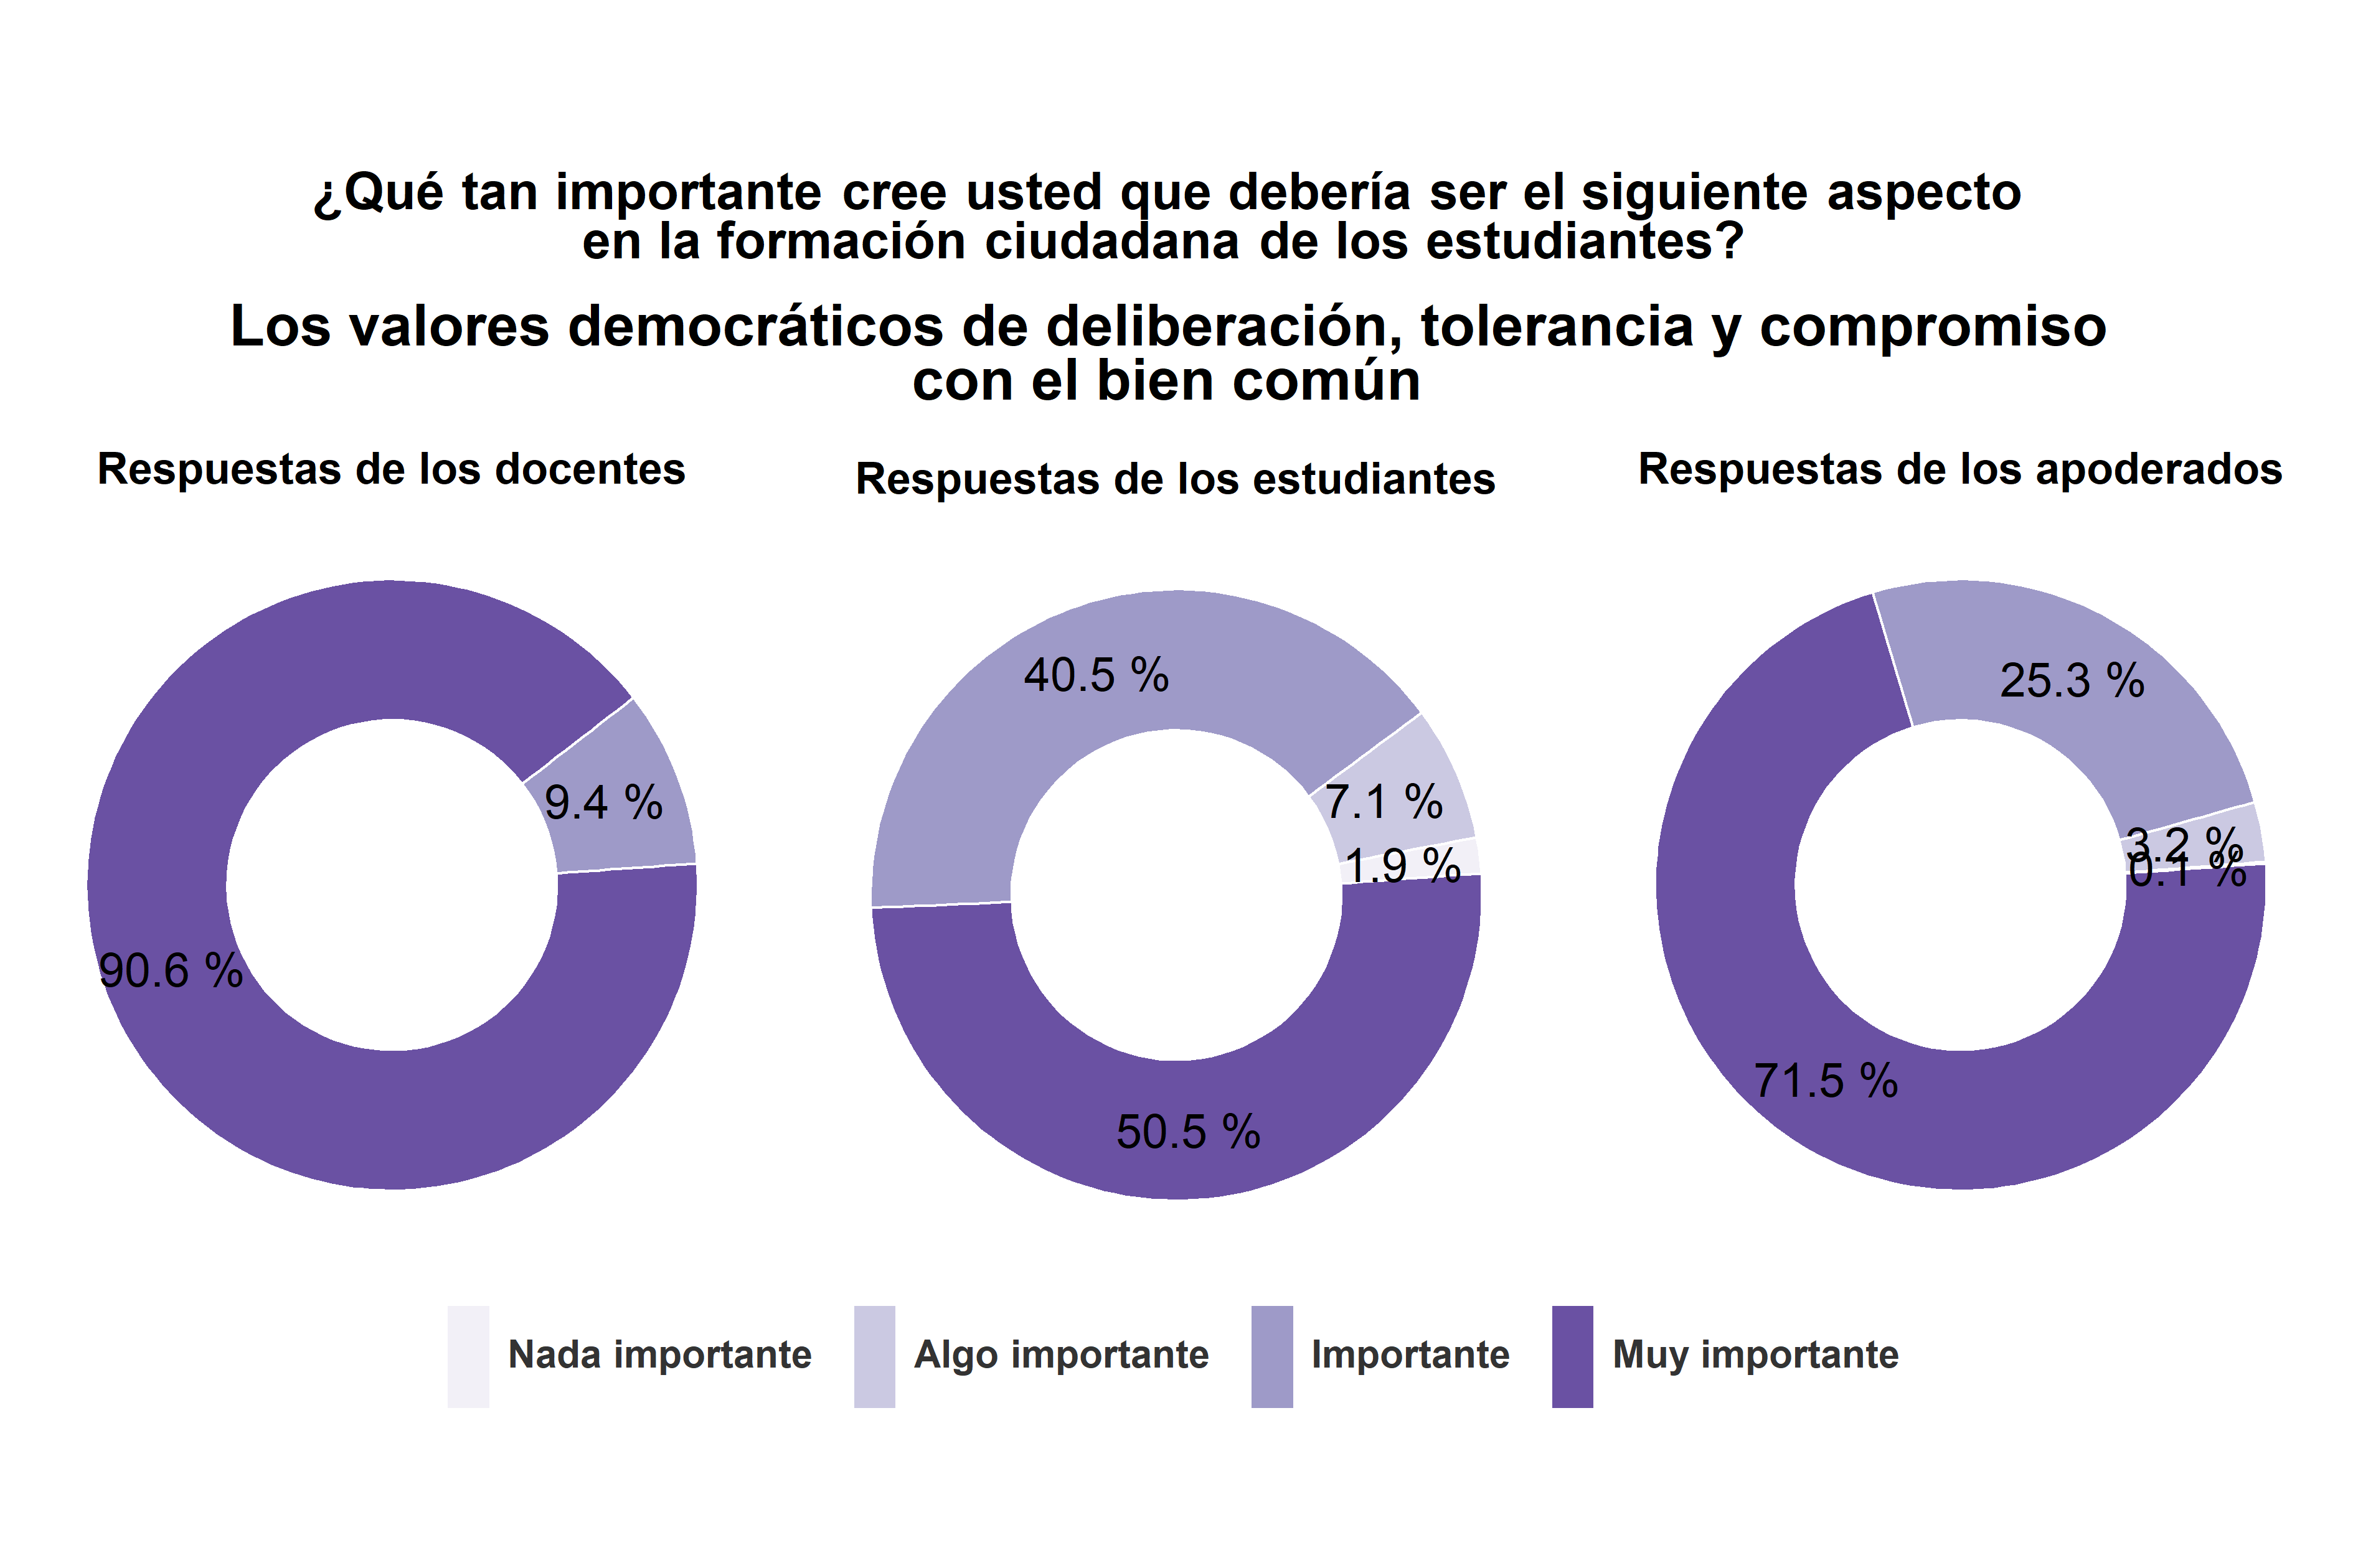
\includegraphics[width=52.49in]{images/graph_for_ciud2} \end{center}

\begin{center}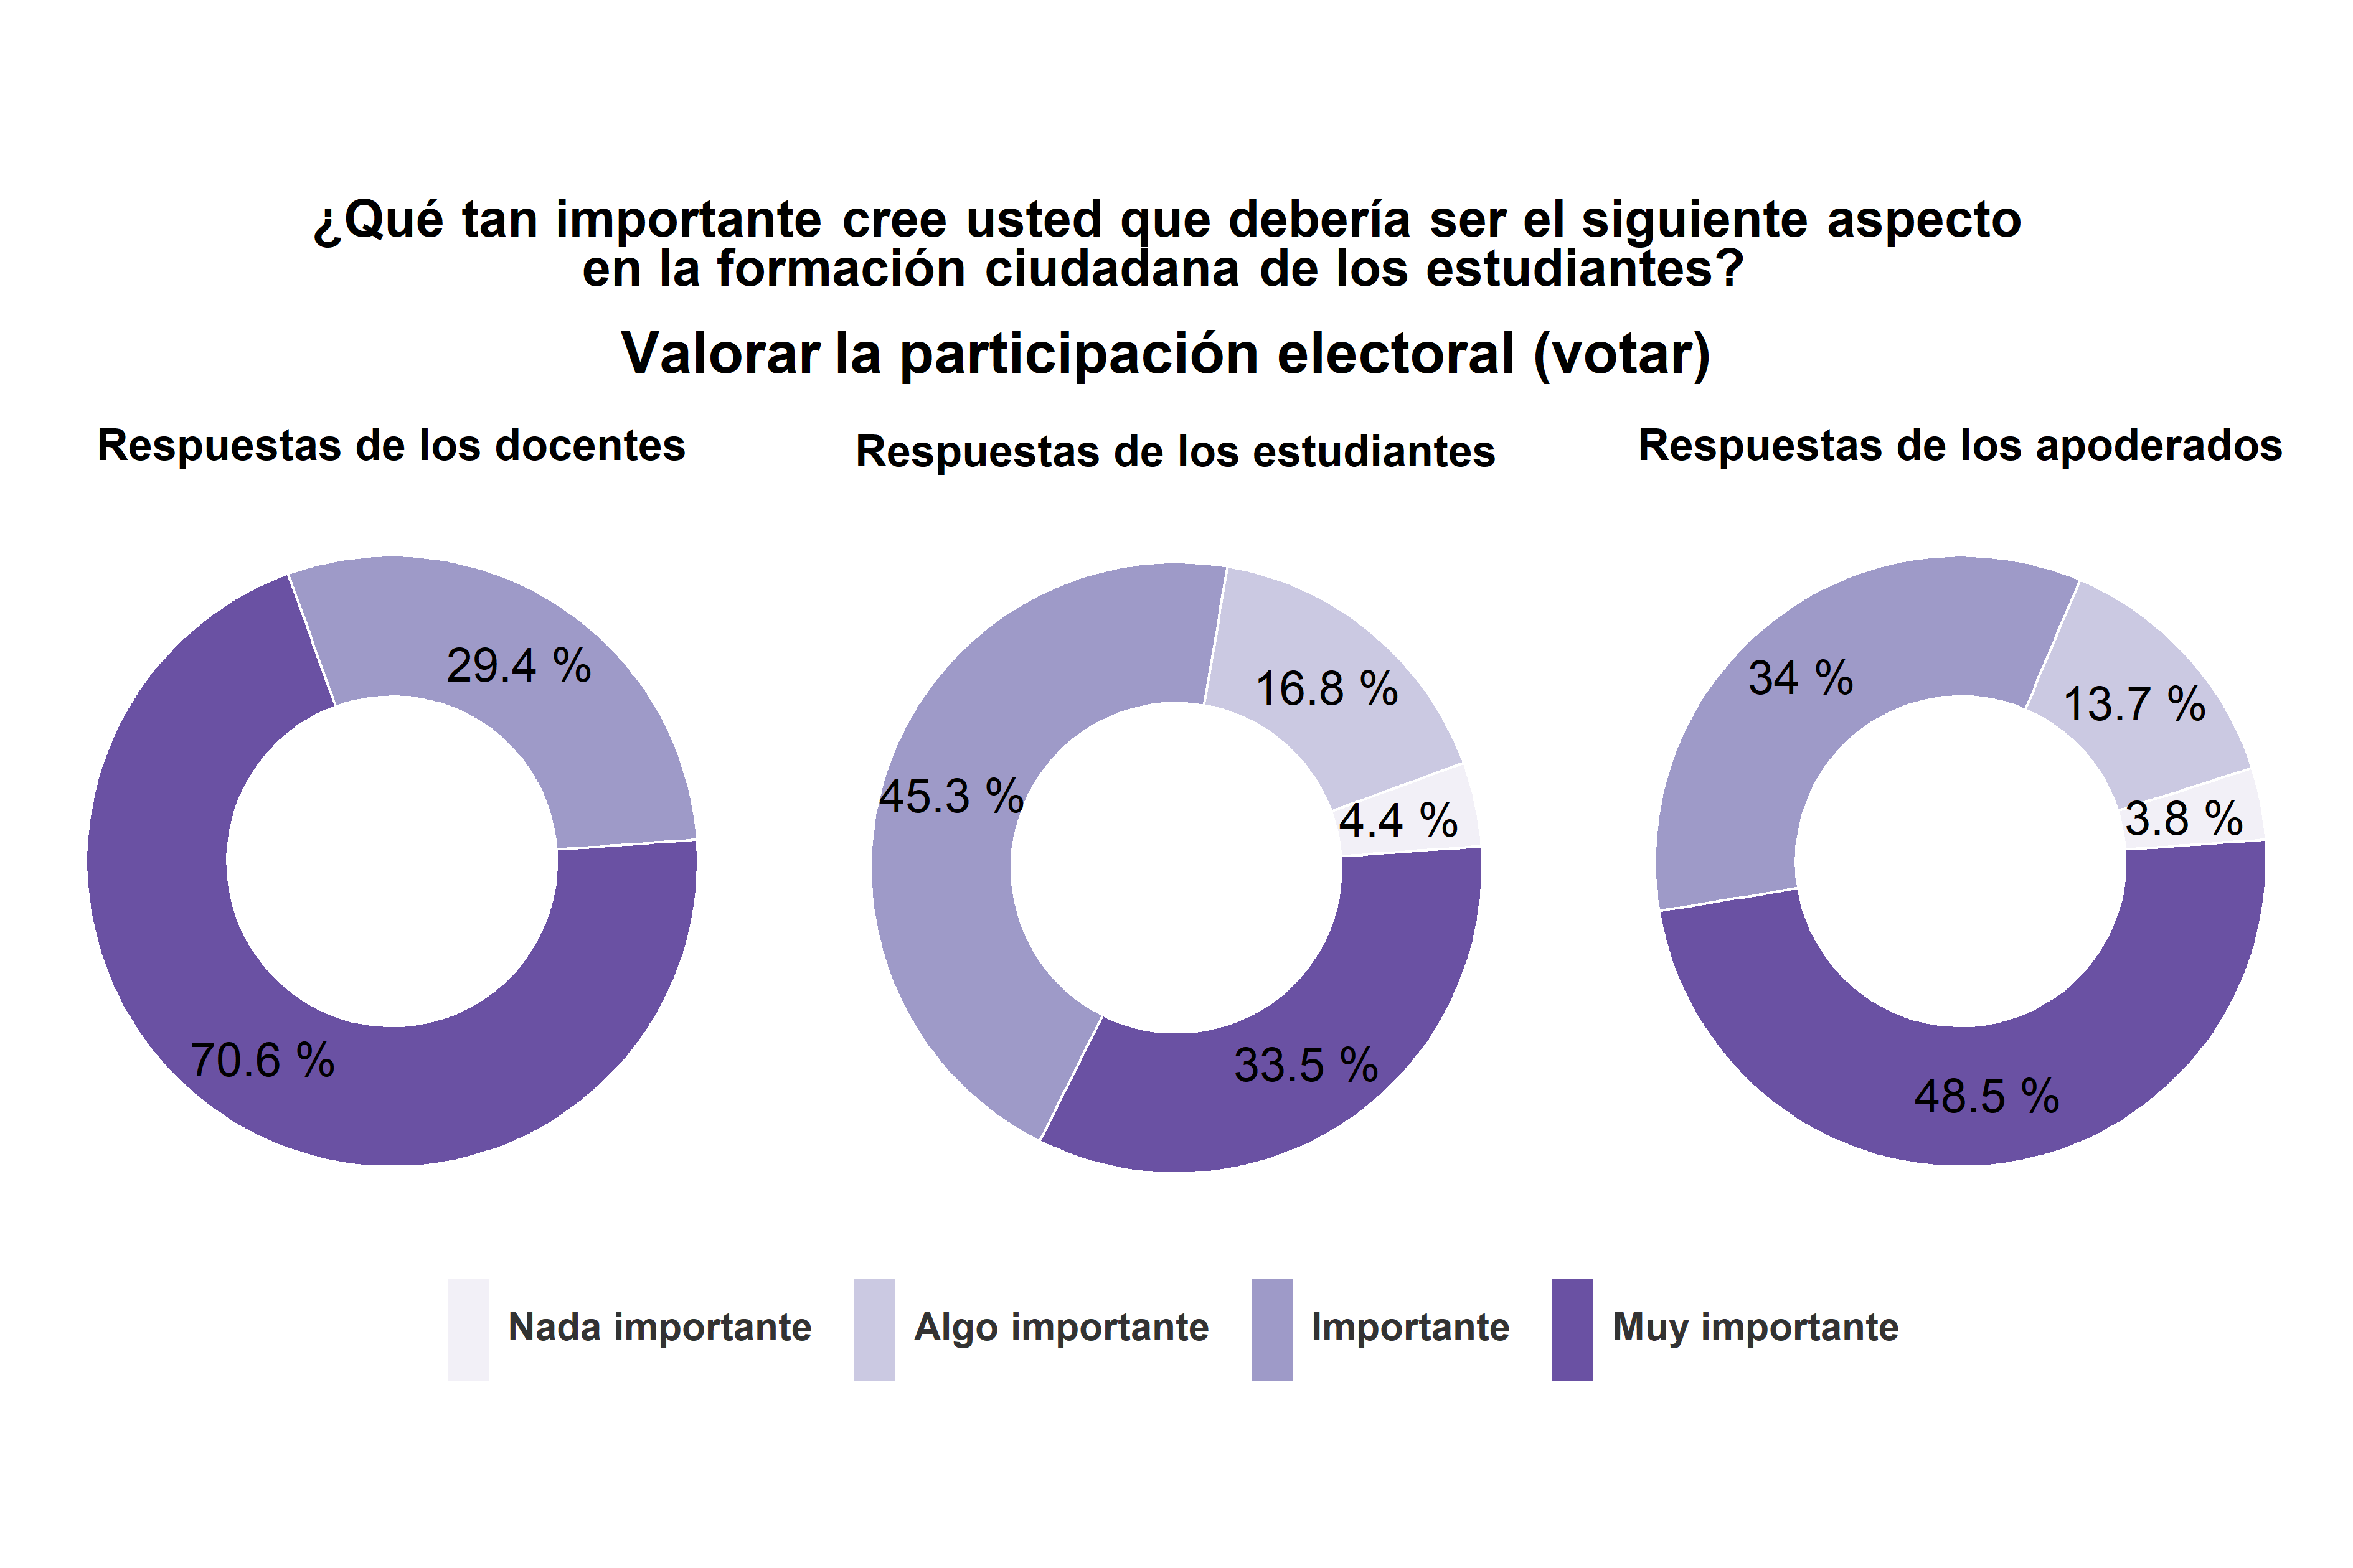
\includegraphics[width=52.49in]{images/graph_for_ciud3} \end{center}

\begin{center}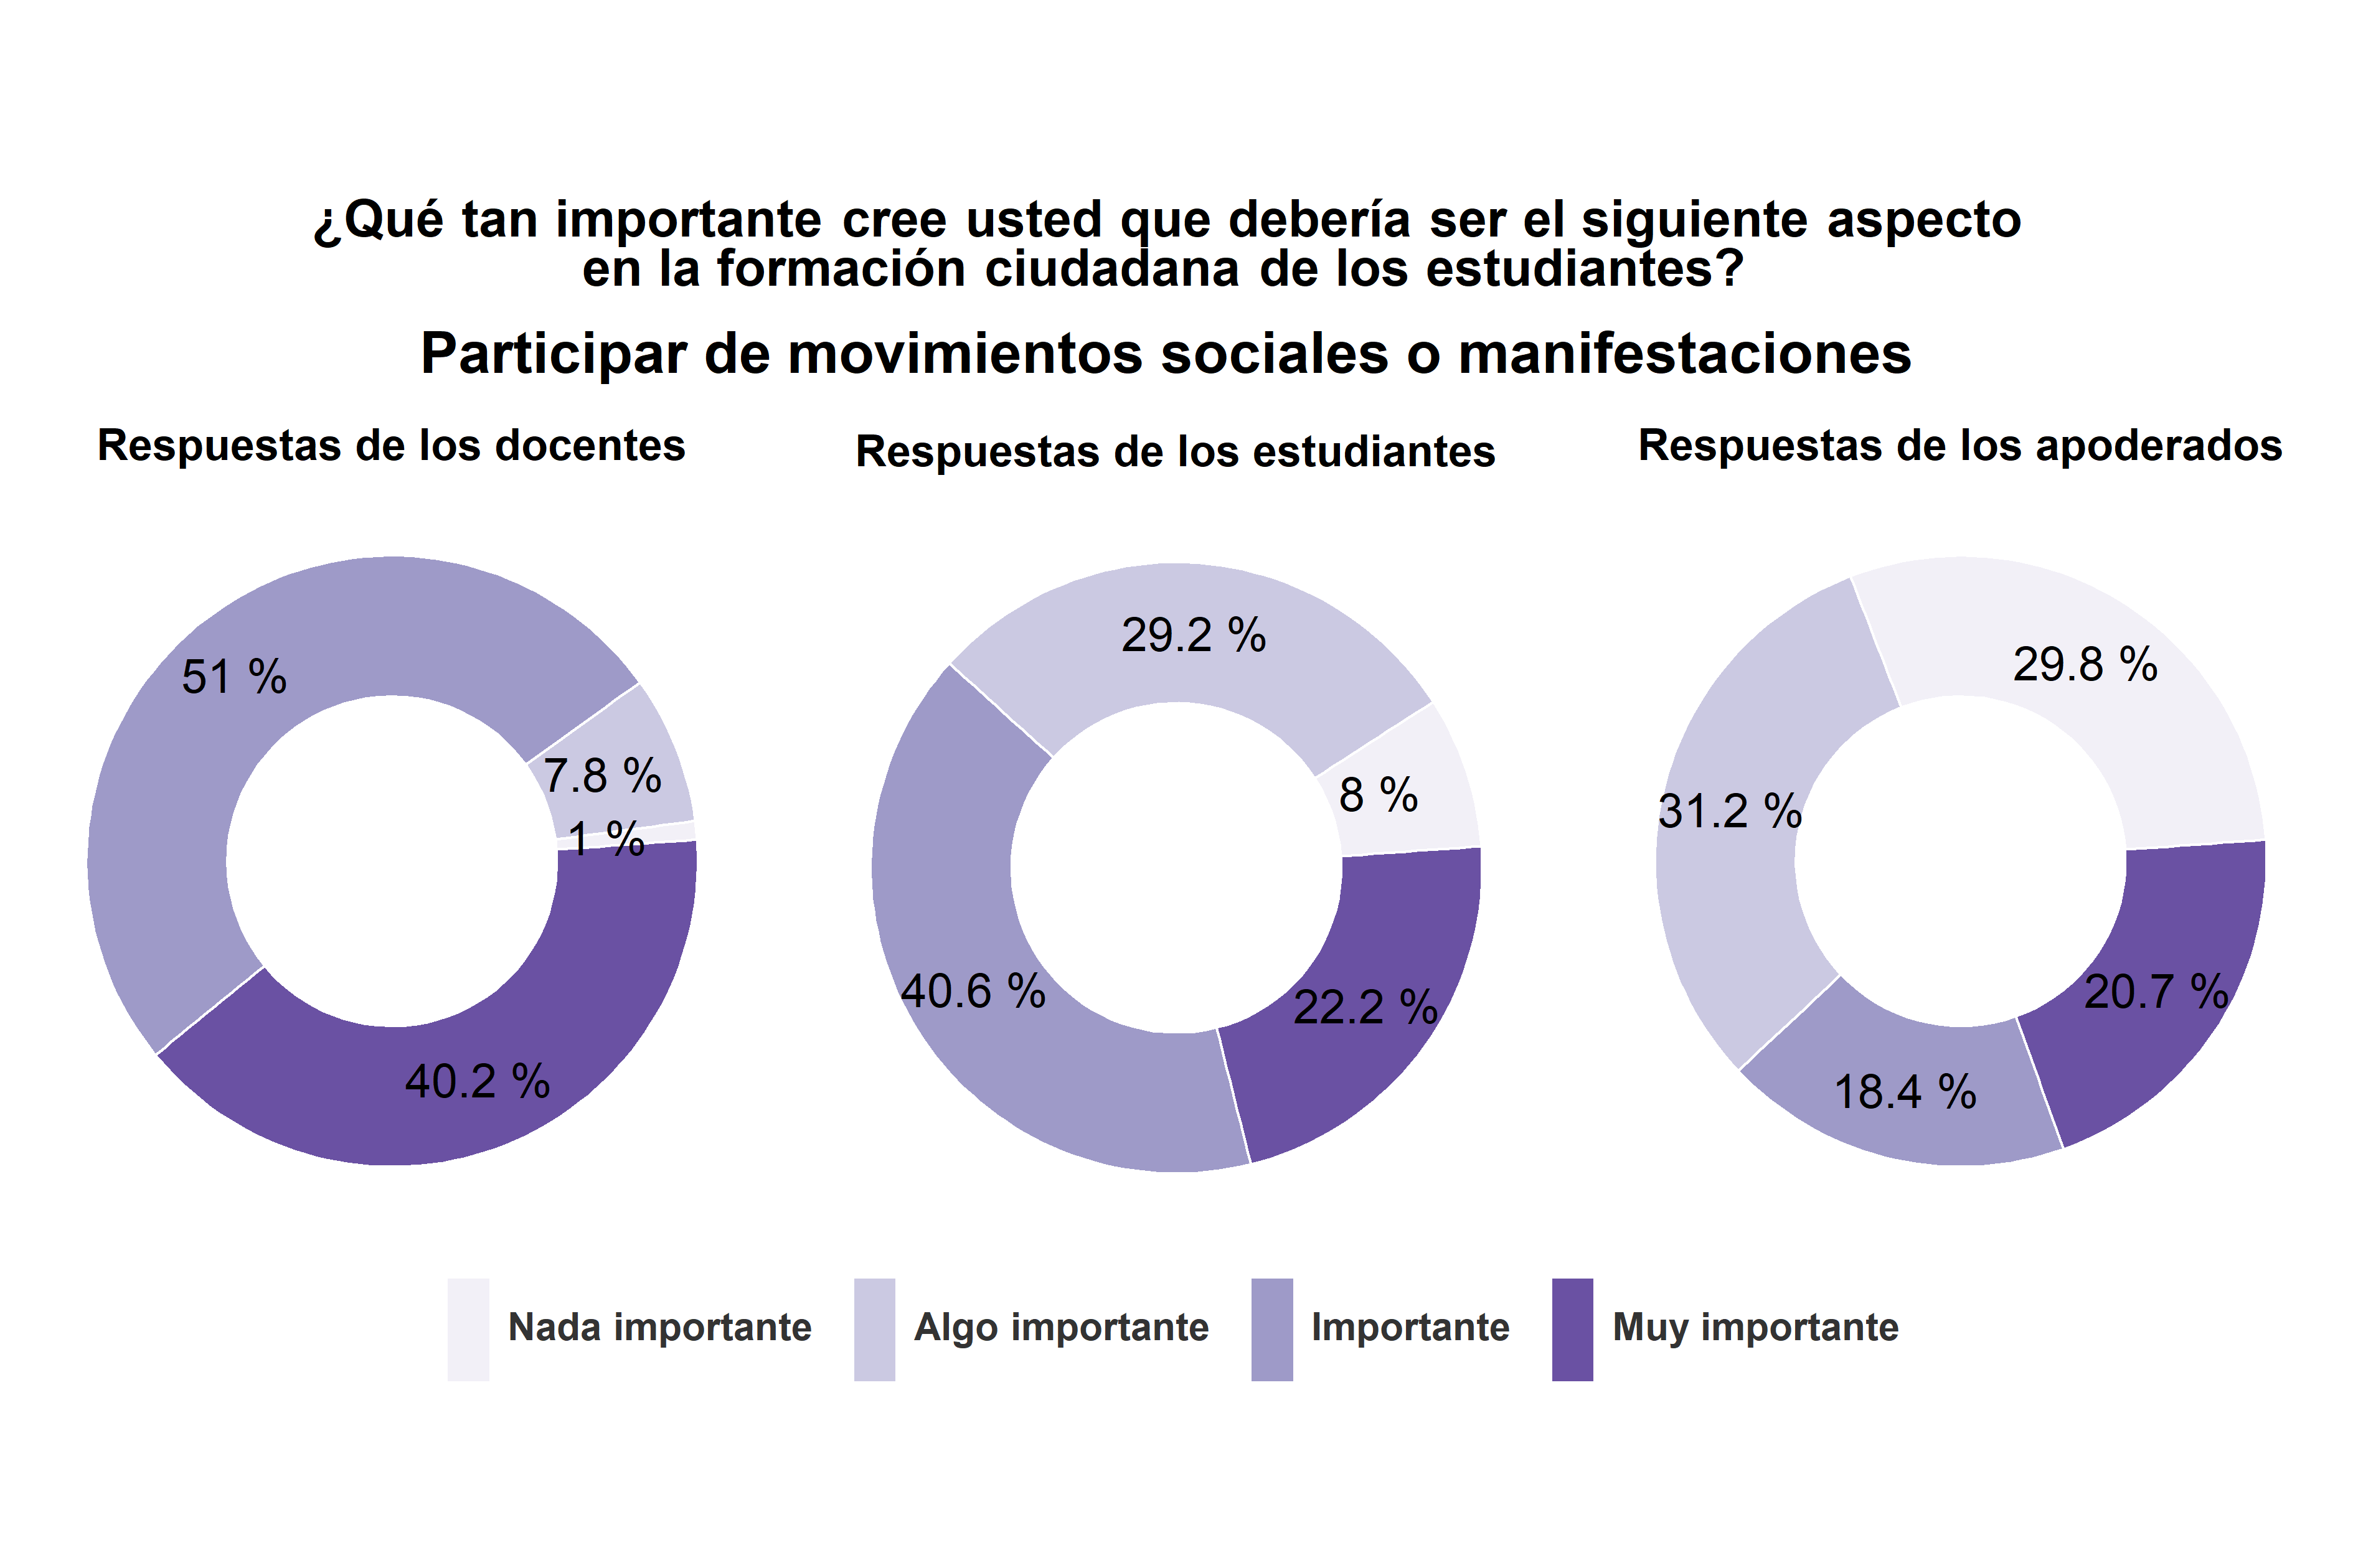
\includegraphics[width=52.49in]{images/graph_for_ciud4} \end{center}

\begin{center}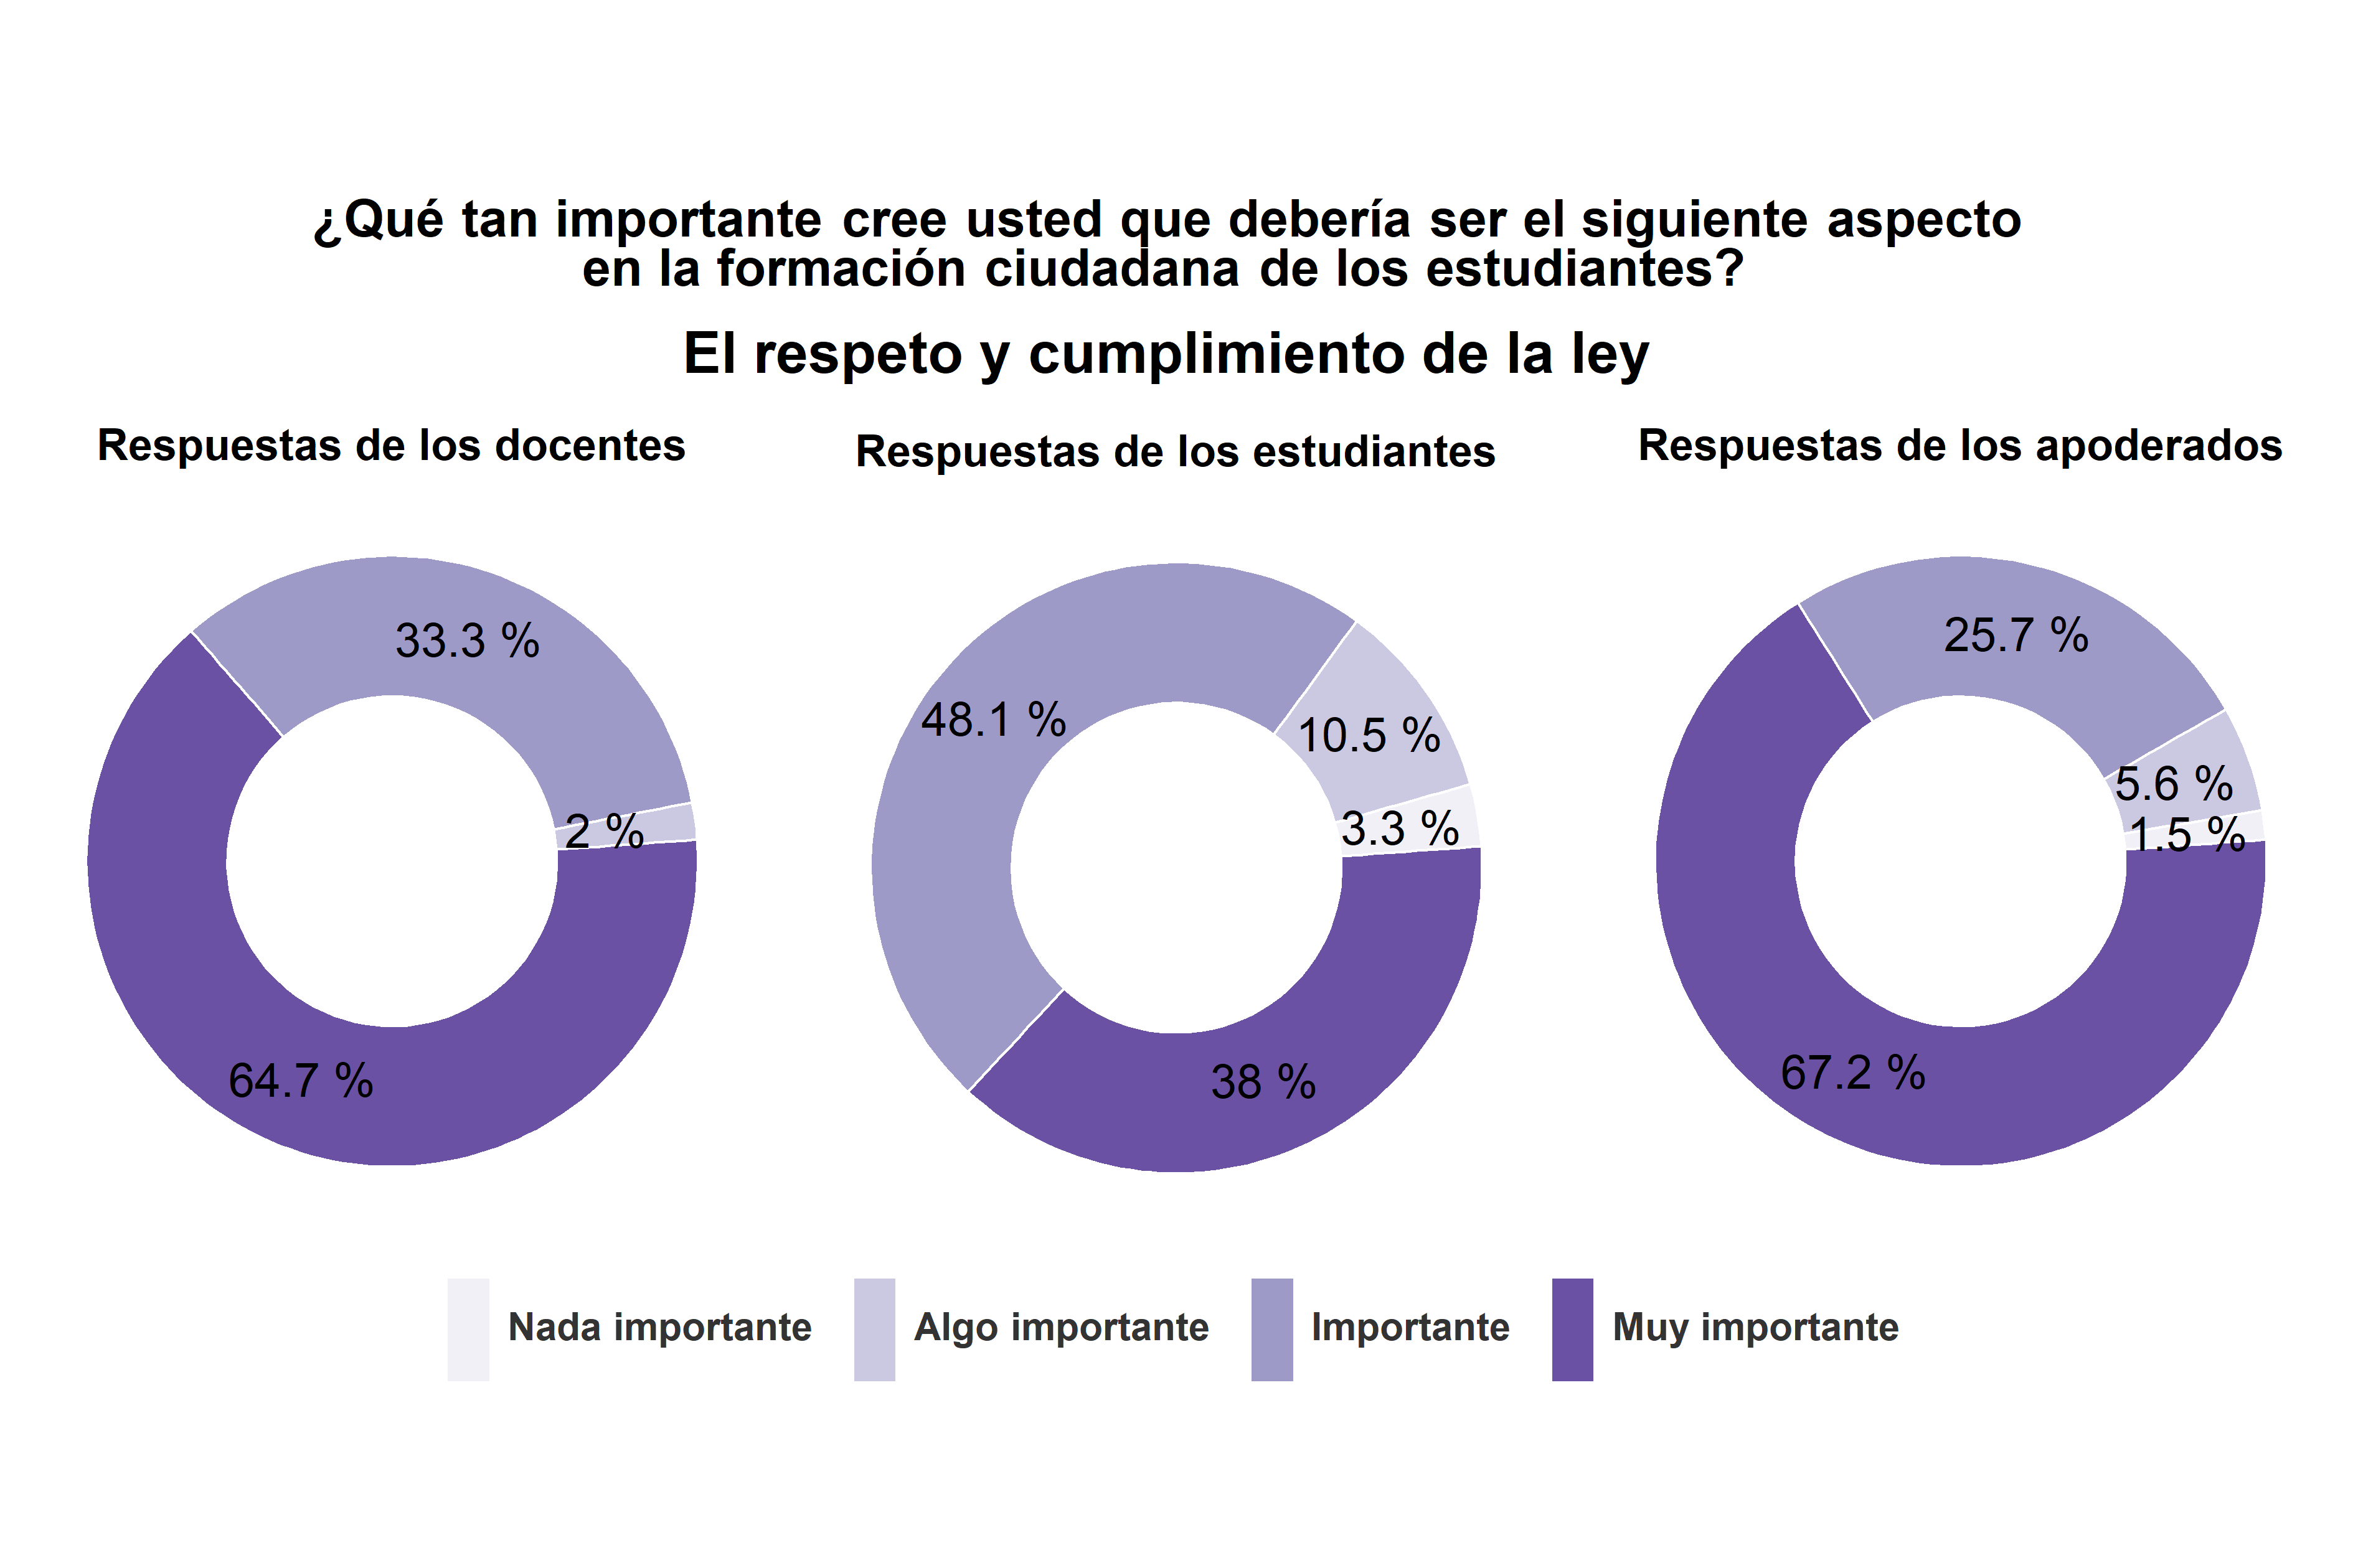
\includegraphics[width=52.49in]{images/graph_for_ciud5} \end{center}

\begin{center}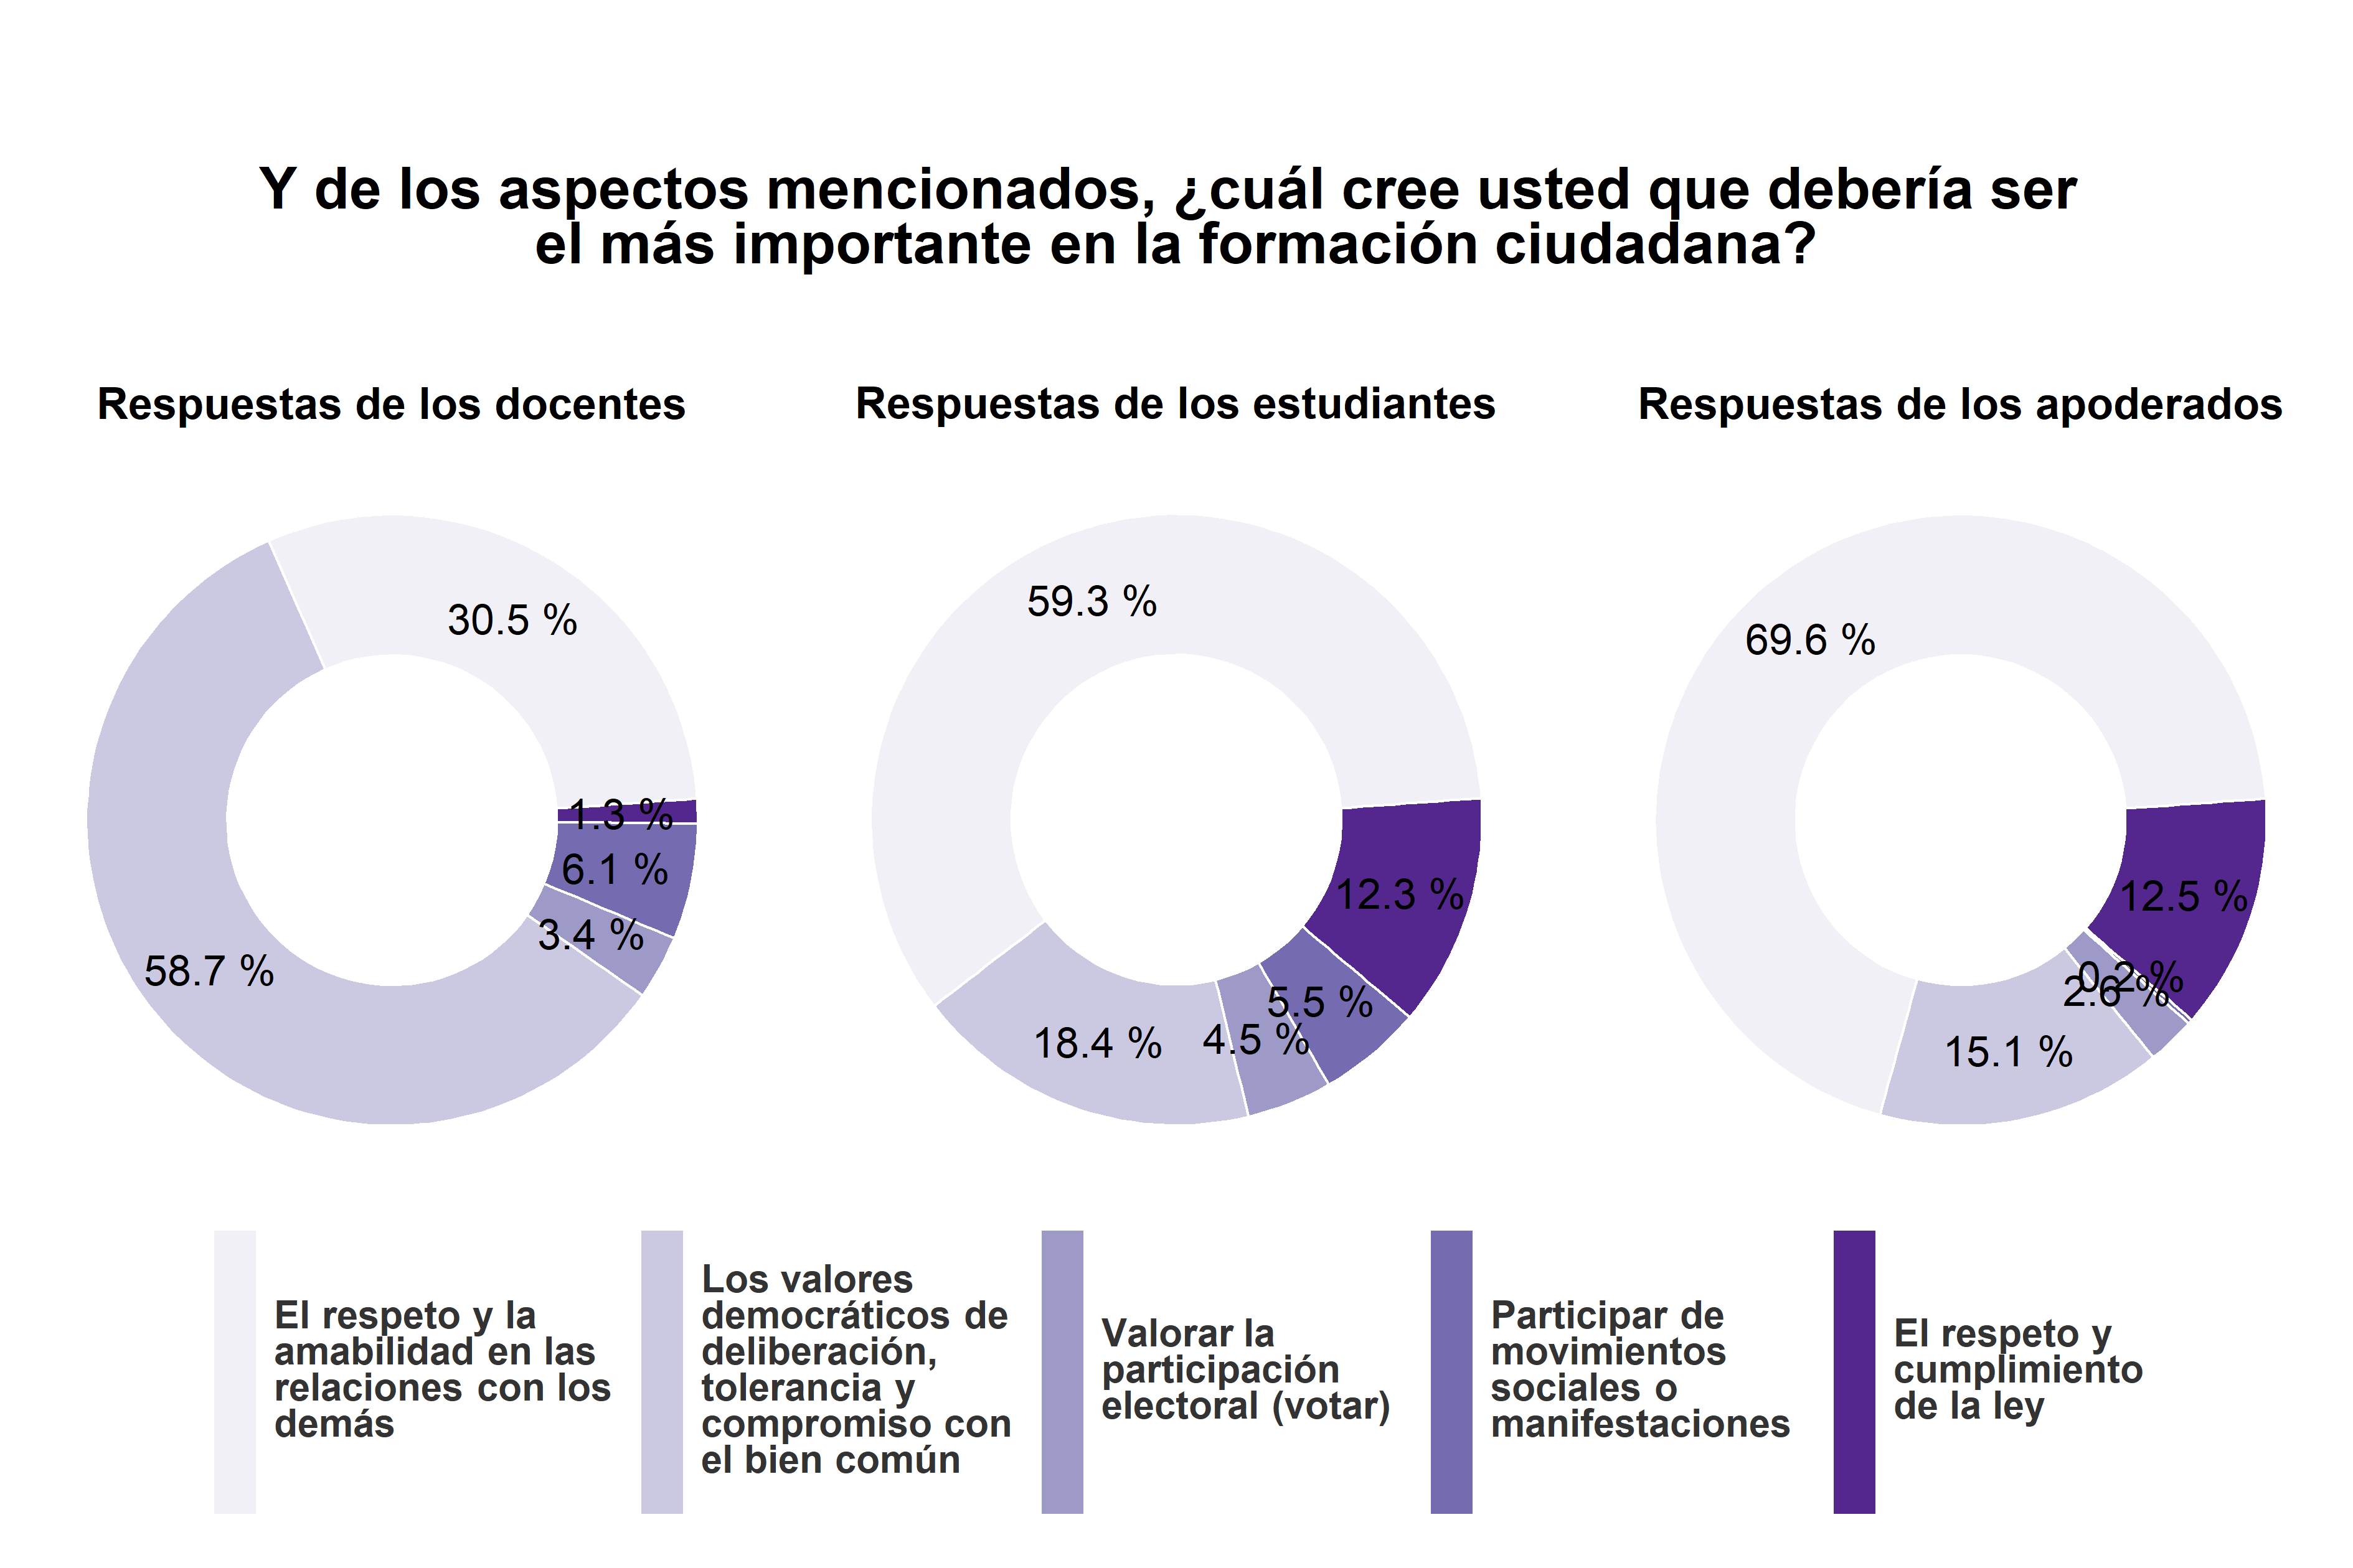
\includegraphics[width=52.49in]{images/graph_for_ciud6} \end{center}

\hypertarget{quiuxe9n-juega-el-rol-muxe1s-importante-en-distintos-aspectos-de-la-formaciuxf3n-ciudadana}{%
\subsection{Quién juega el rol más importante en distintos aspectos de la formación ciudadana}\label{quiuxe9n-juega-el-rol-muxe1s-importante-en-distintos-aspectos-de-la-formaciuxf3n-ciudadana}}

\begin{center}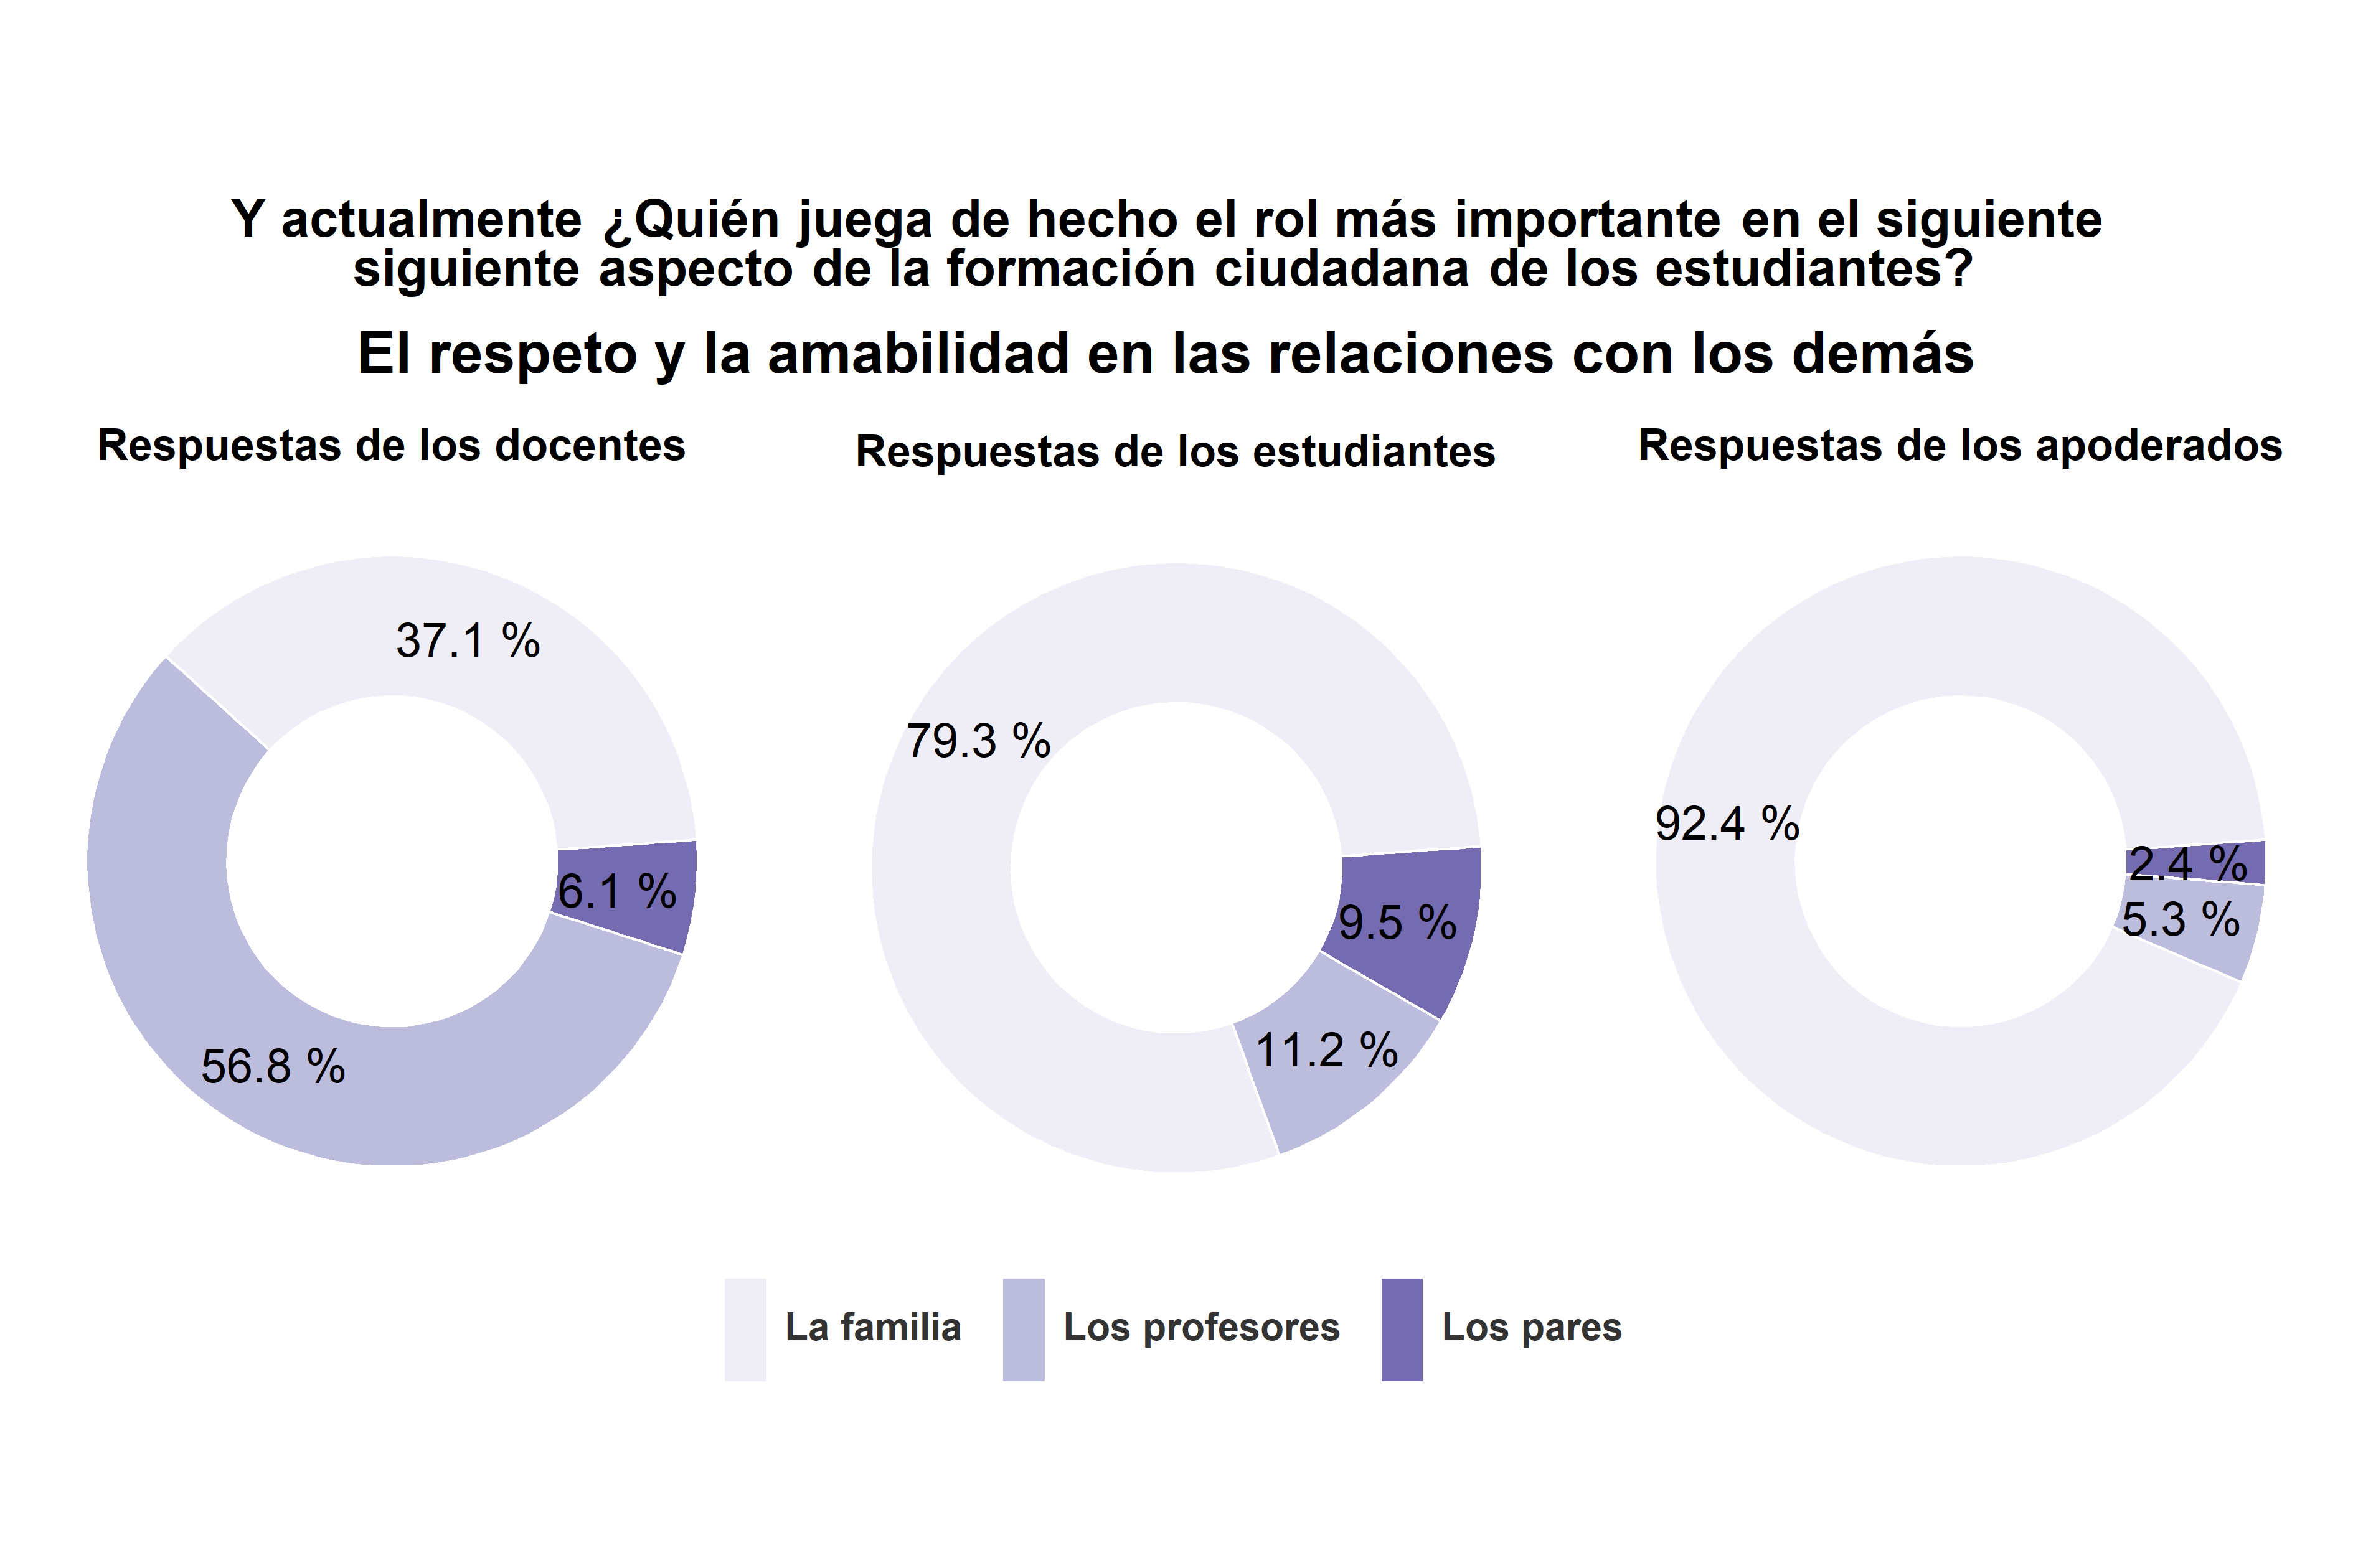
\includegraphics[width=52.49in]{images/graph_for_ciud7} \end{center}

\begin{center}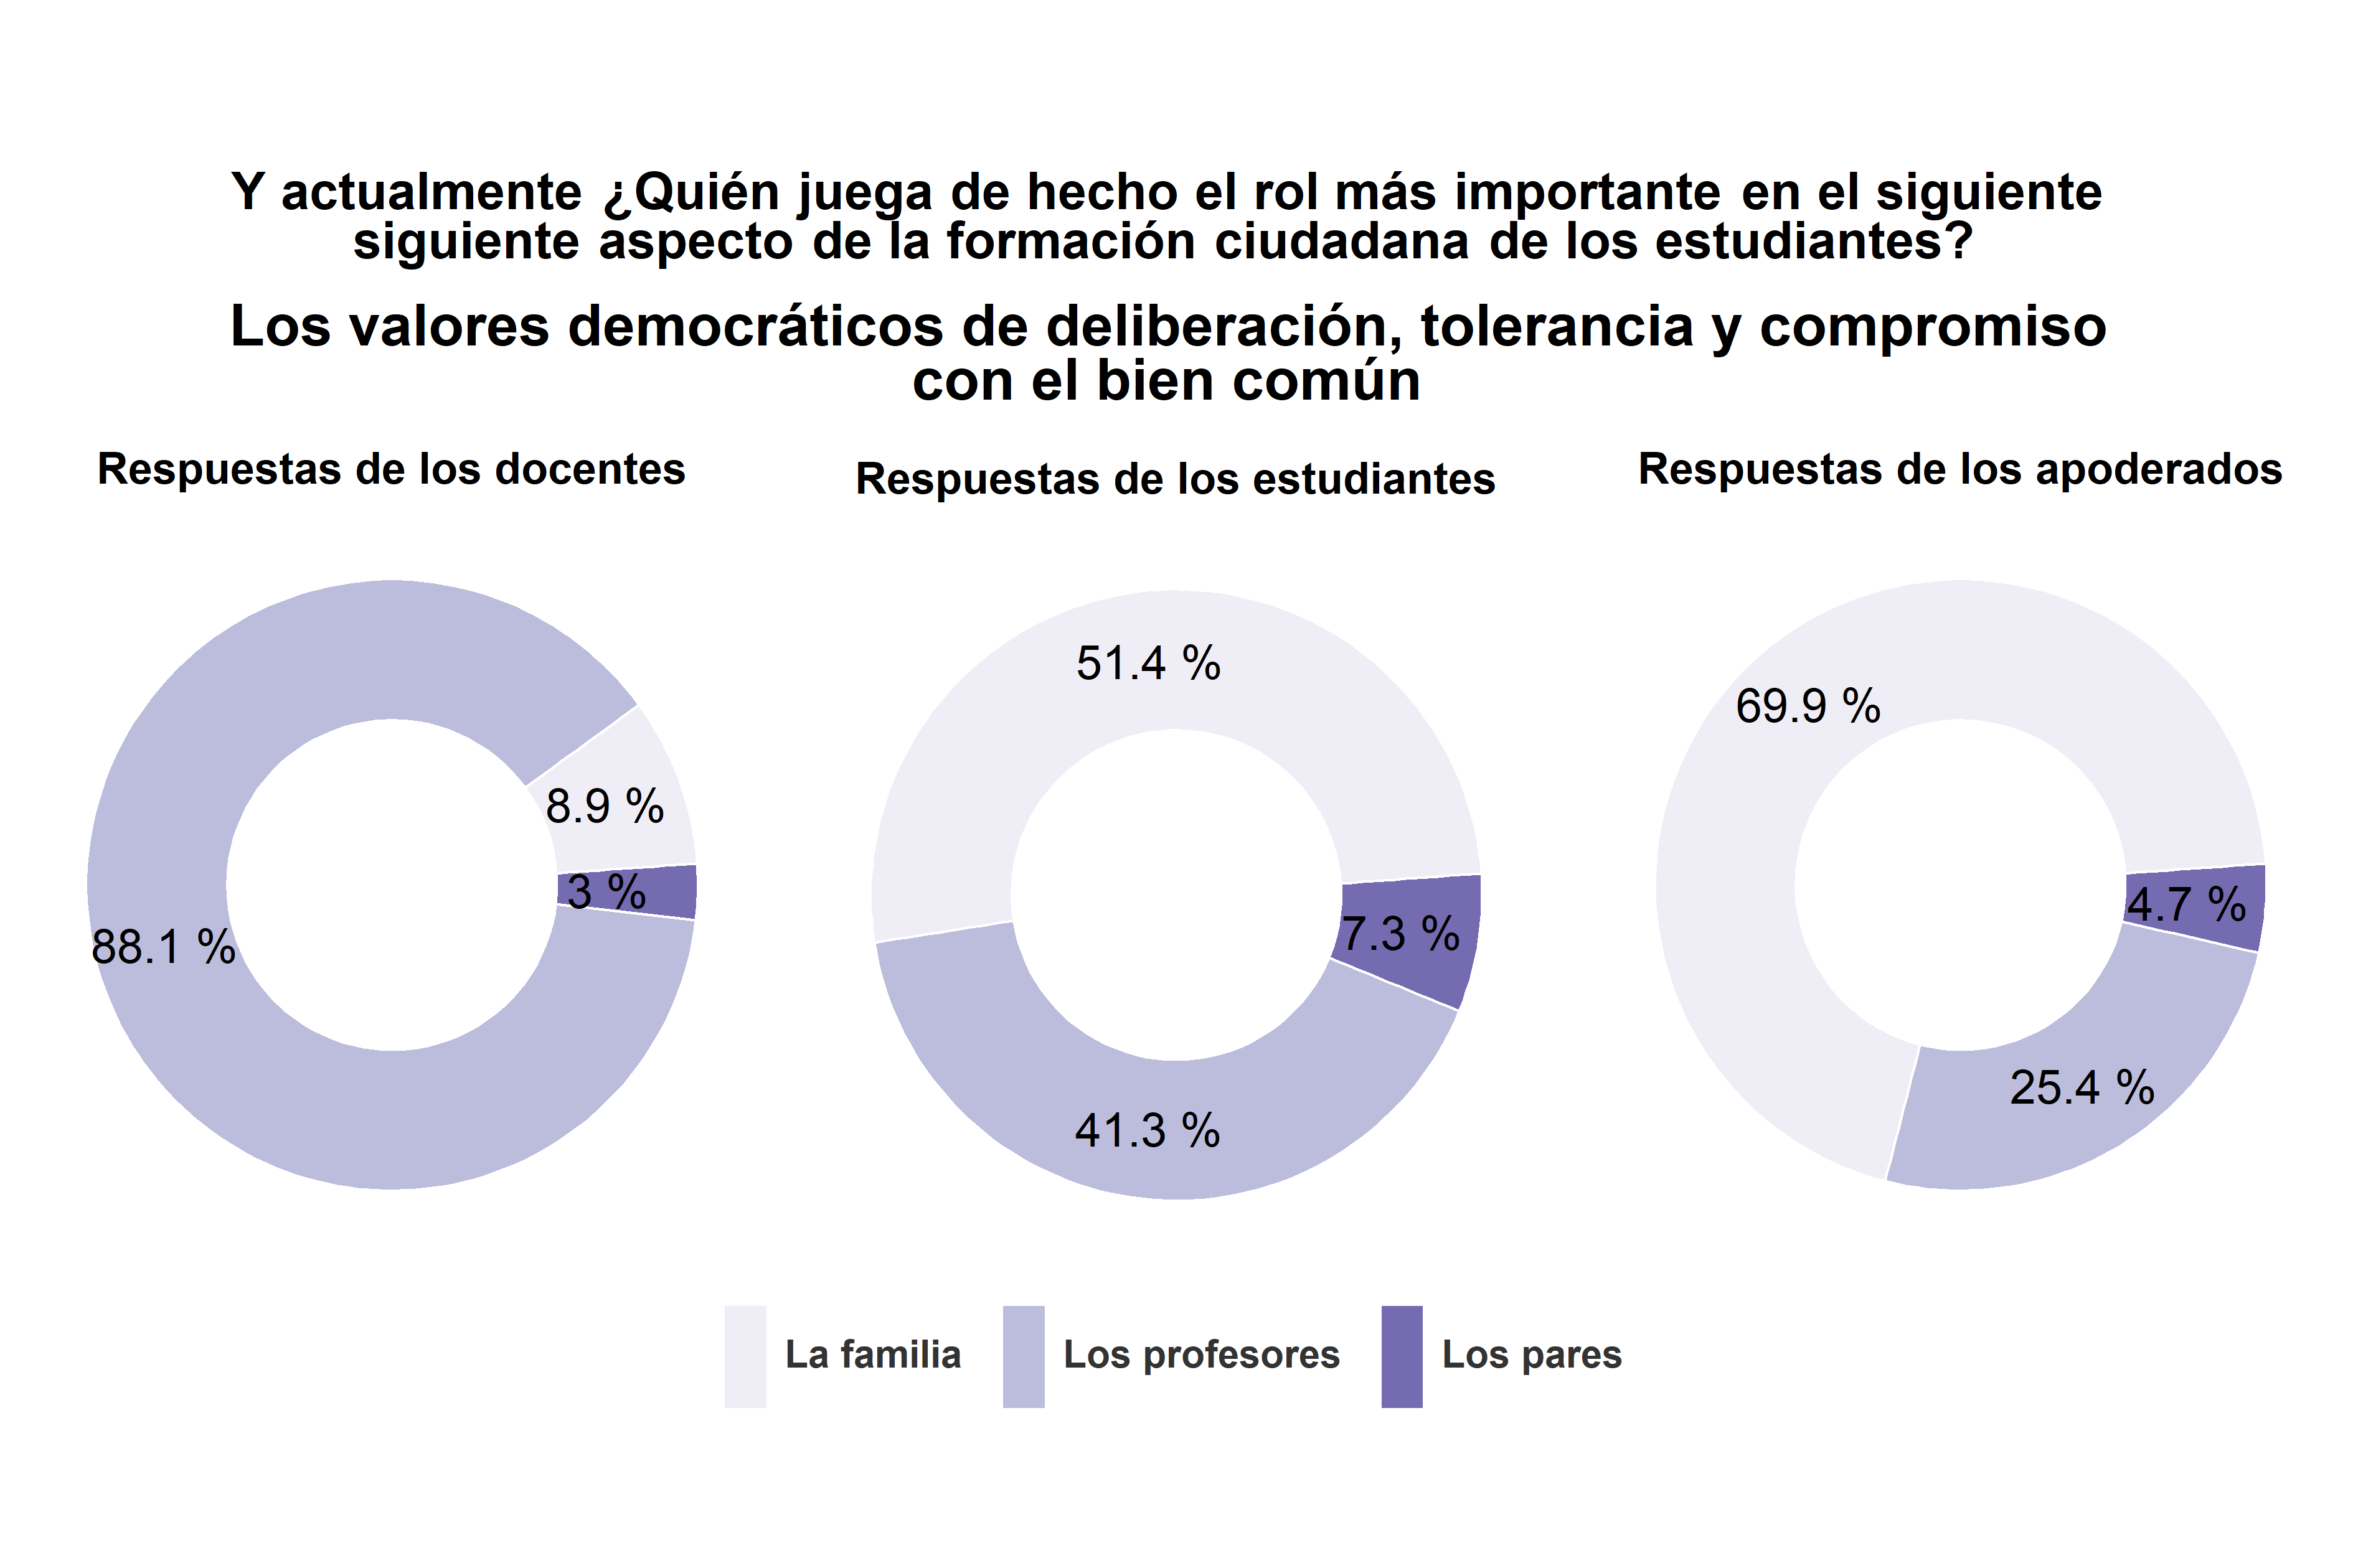
\includegraphics[width=52.49in]{images/graph_for_ciud8} \end{center}

\begin{center}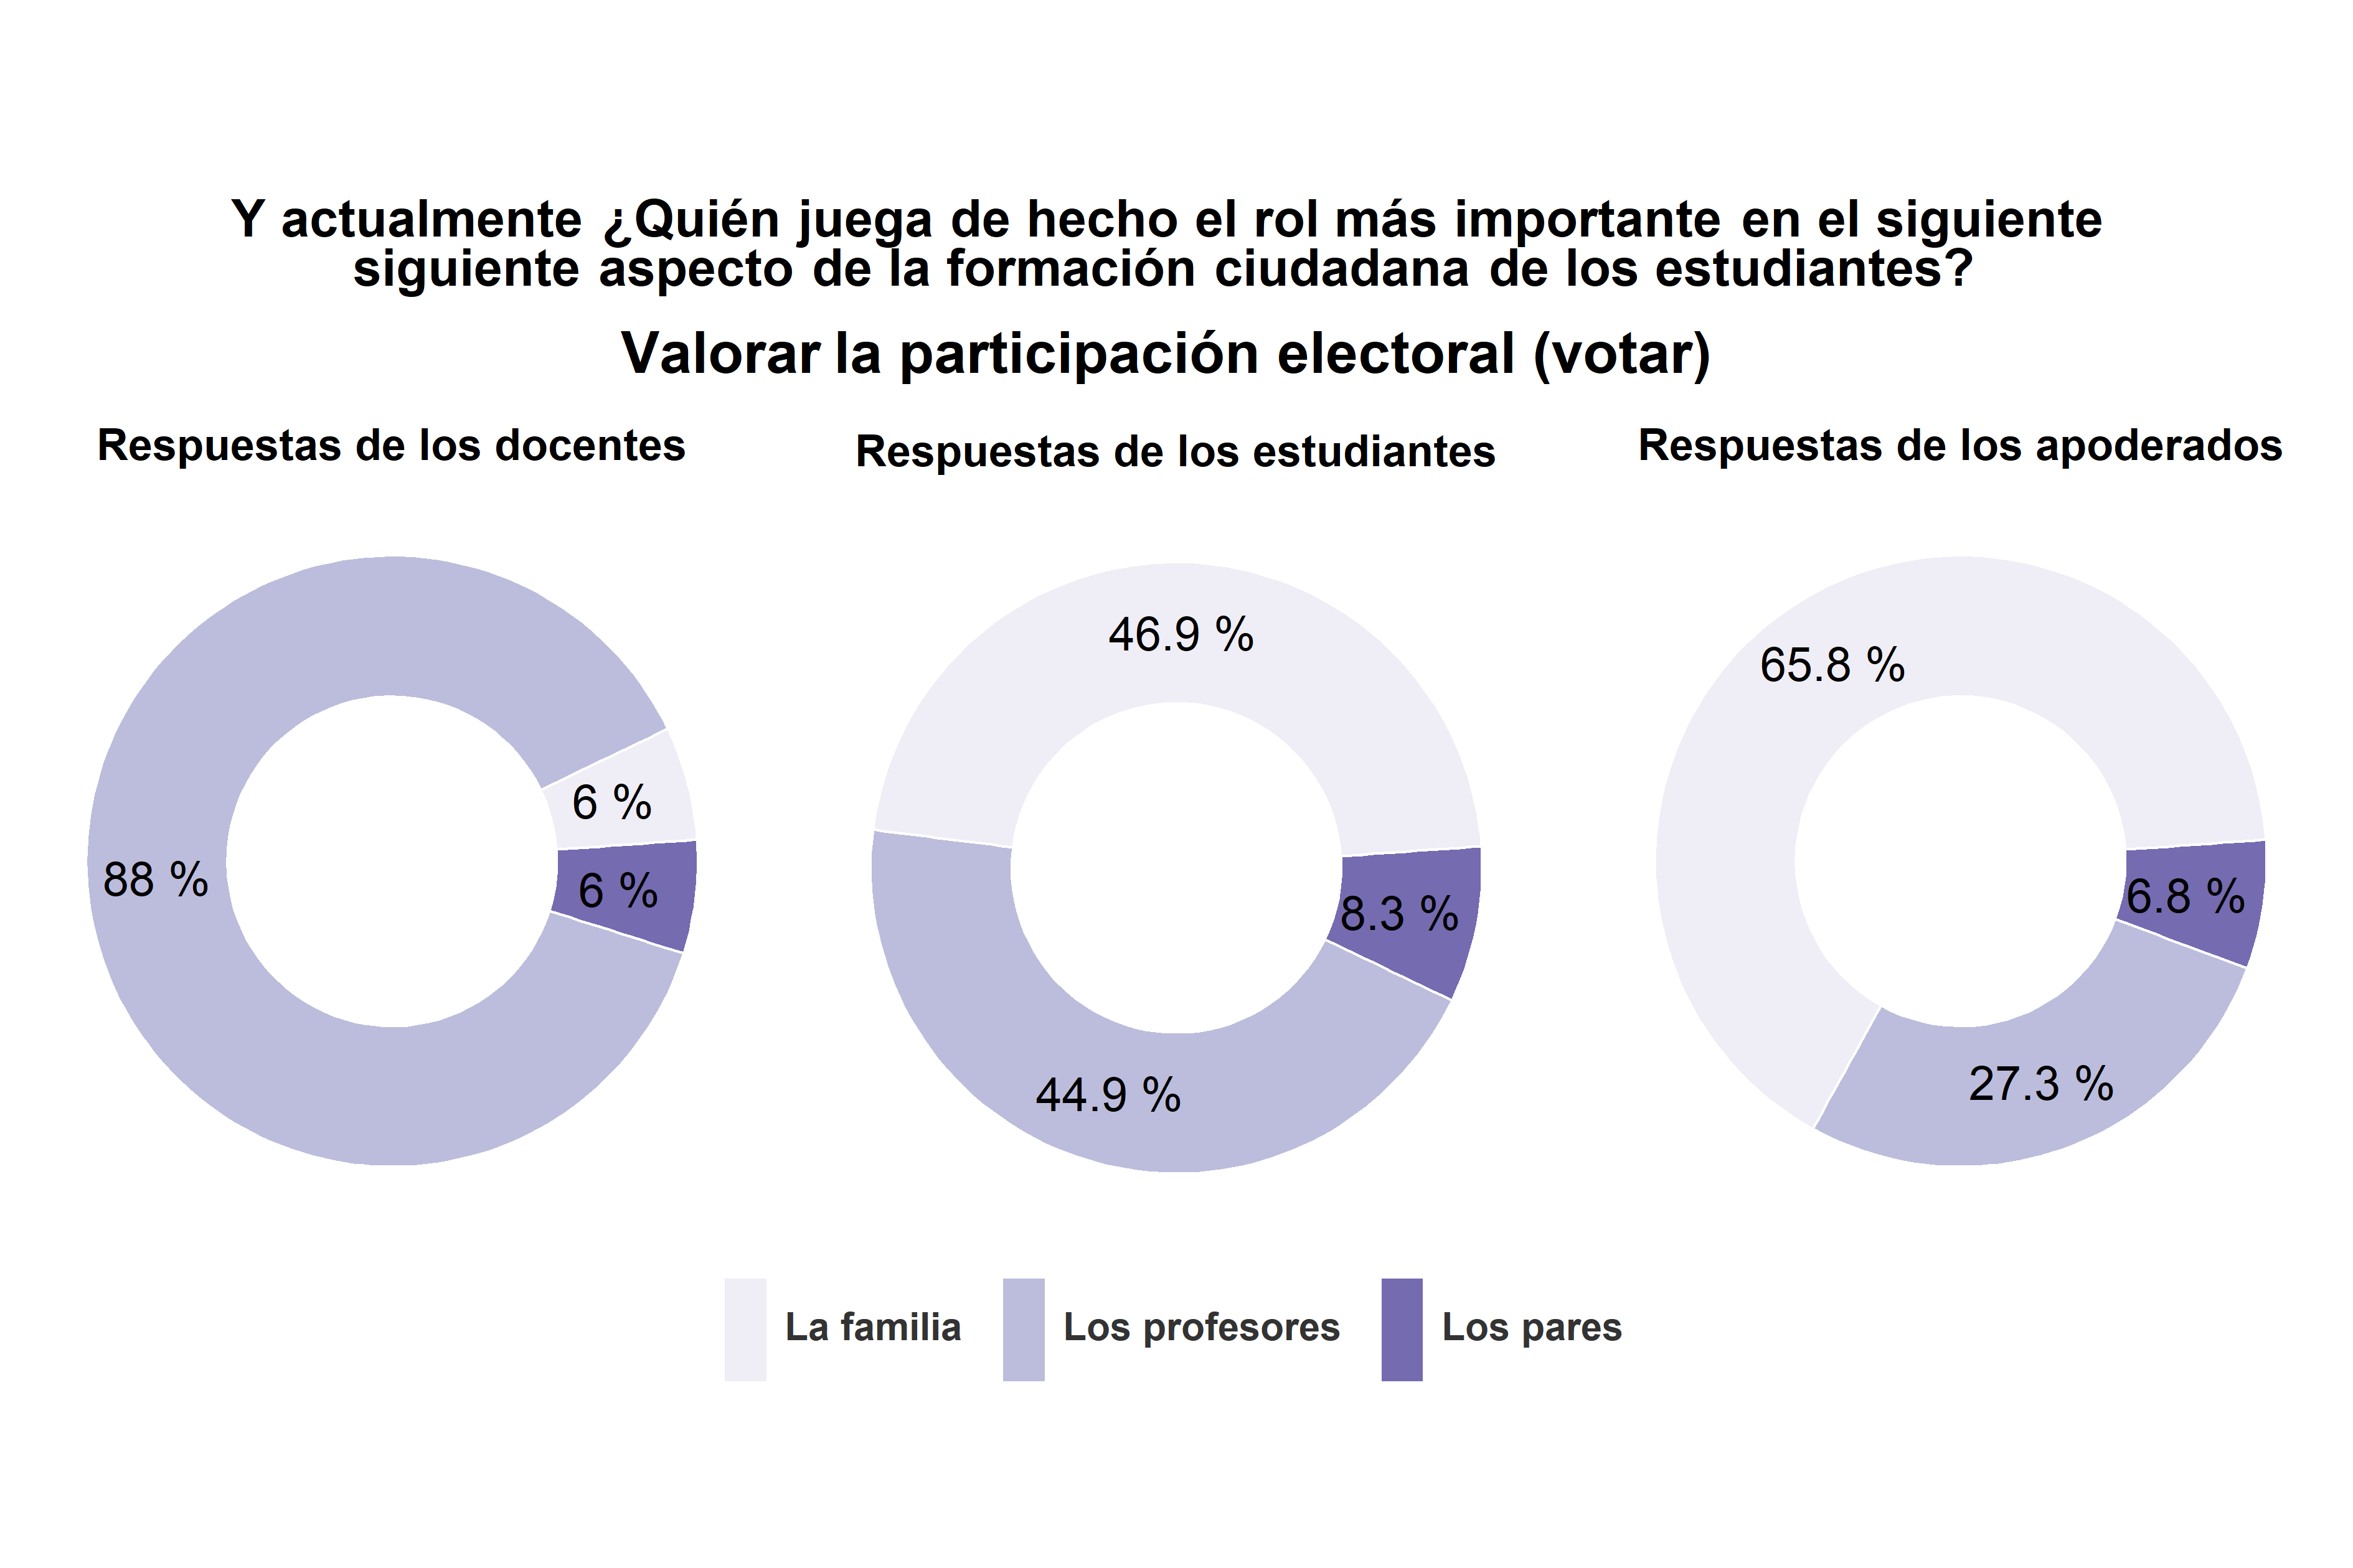
\includegraphics[width=52.49in]{images/graph_for_ciud9} \end{center}

\begin{center}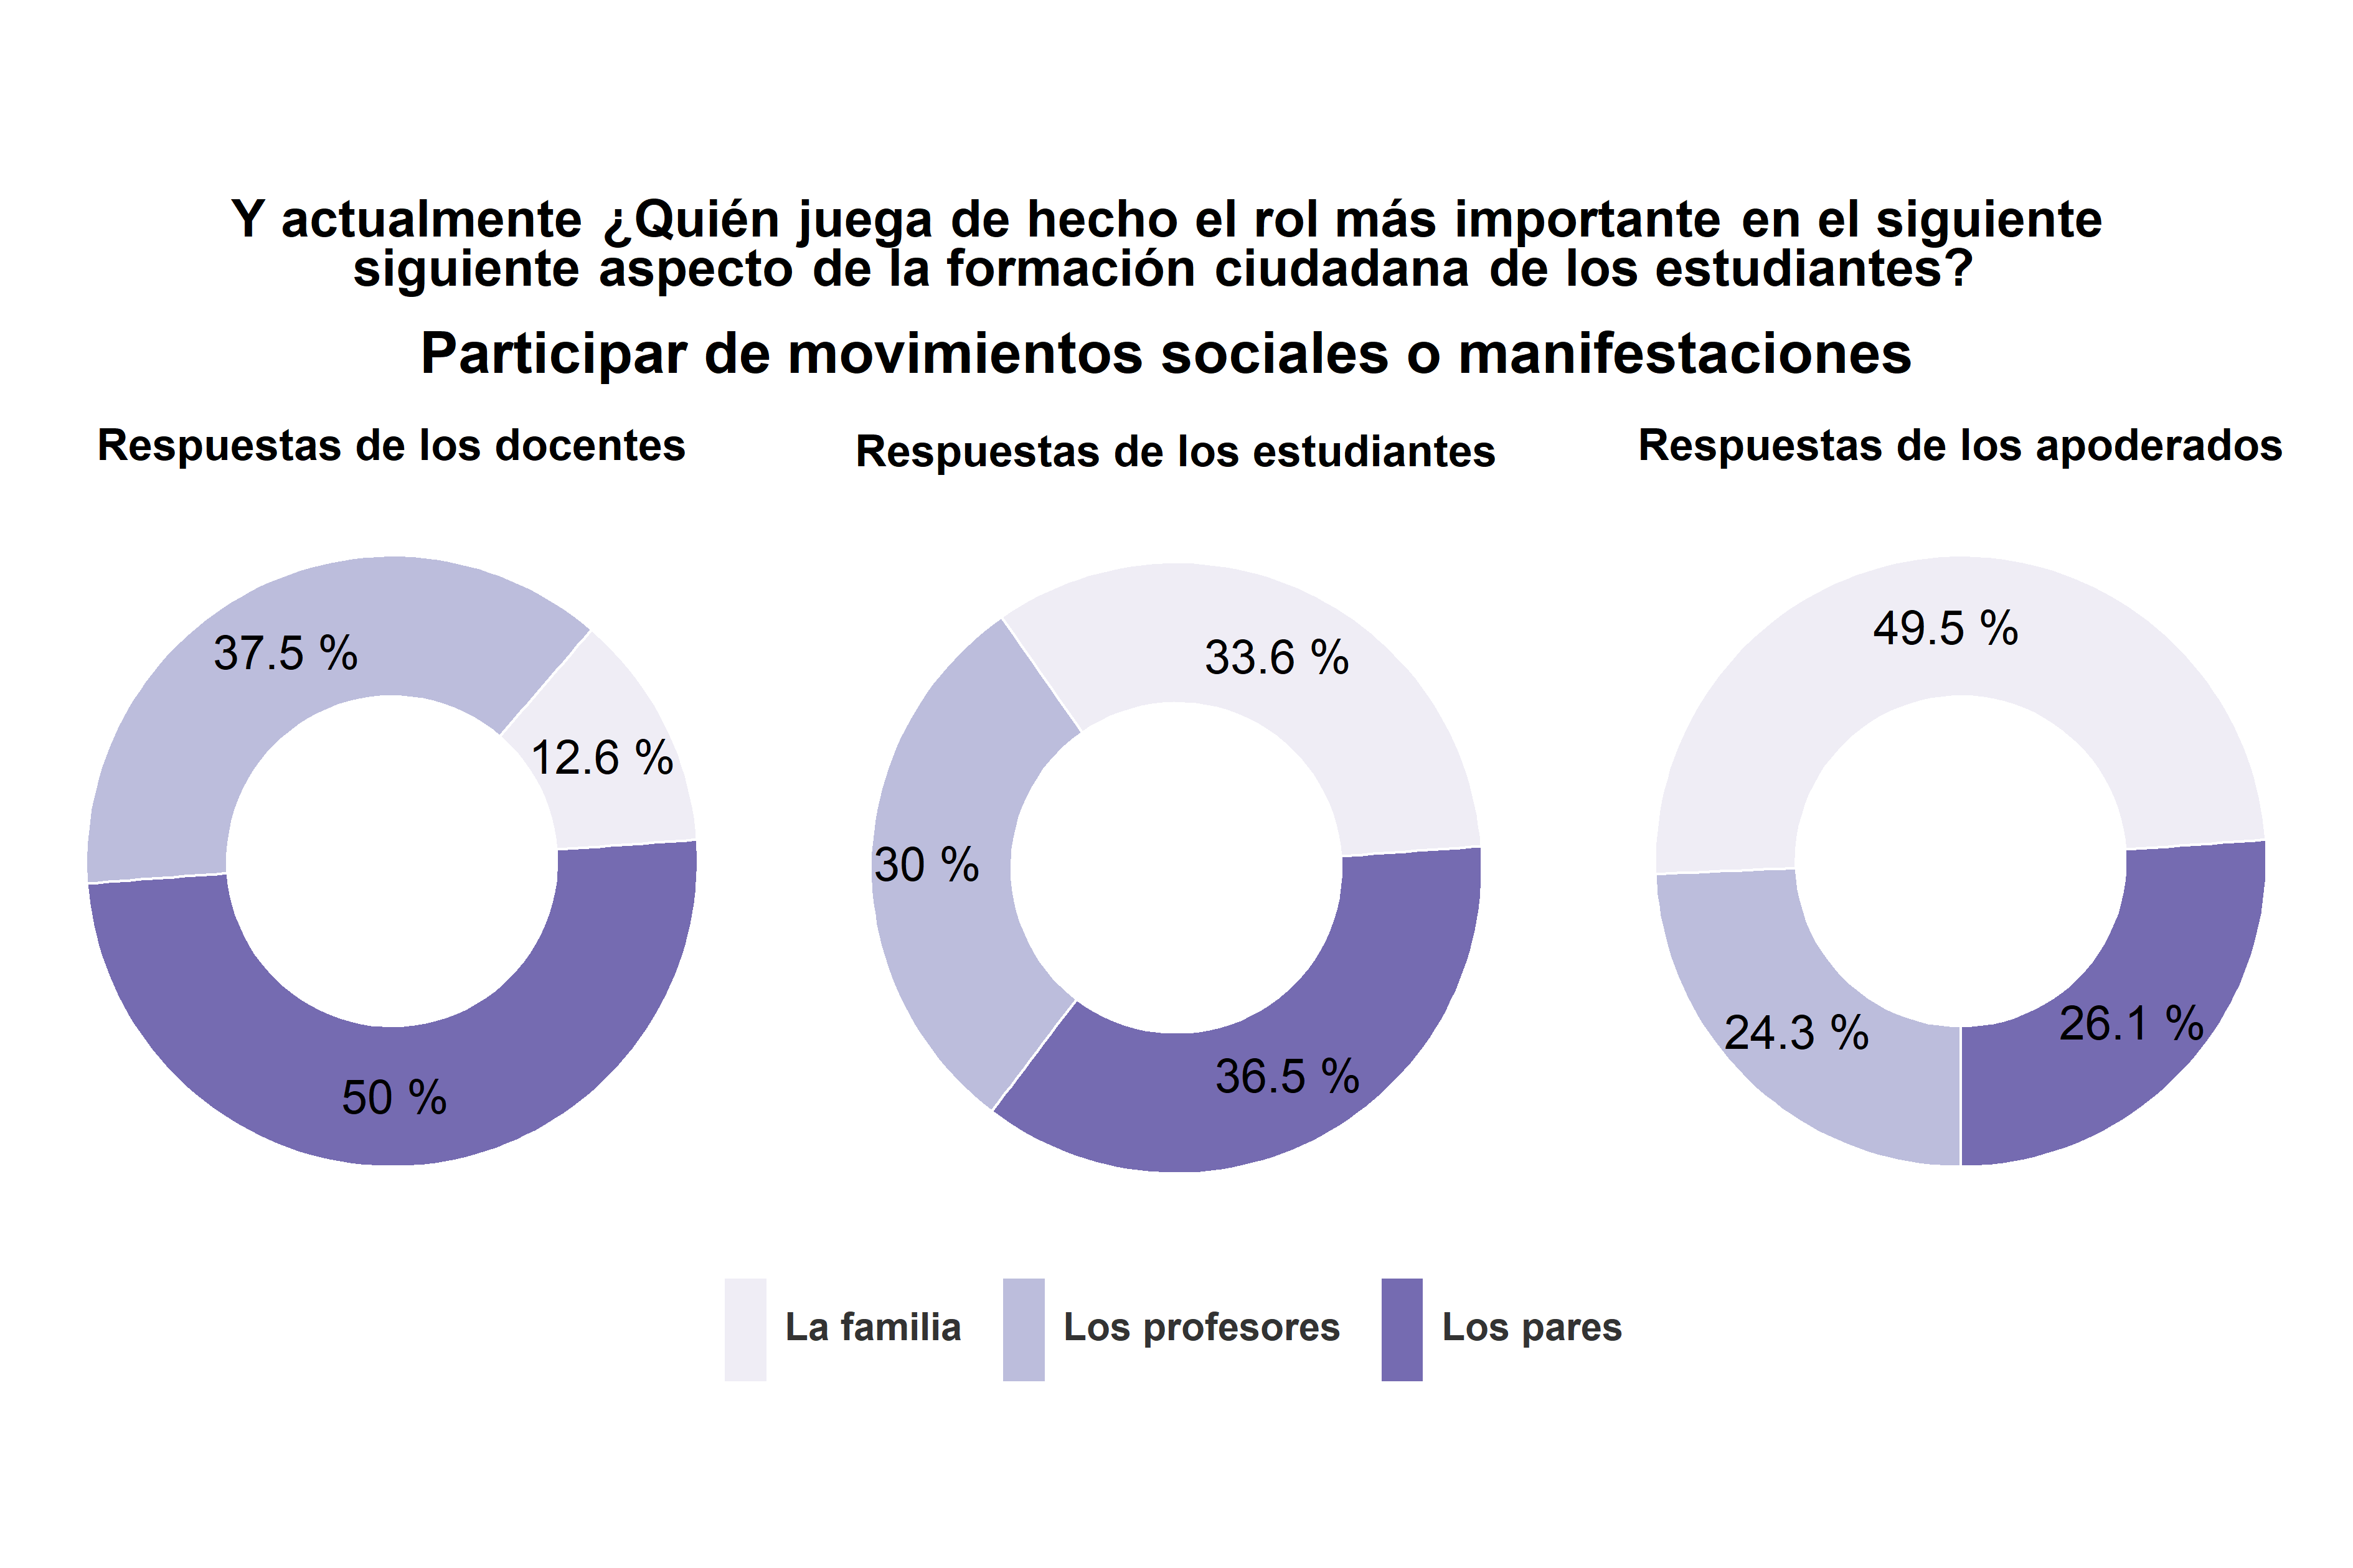
\includegraphics[width=52.49in]{images/graph_for_ciud10} \end{center}

\begin{center}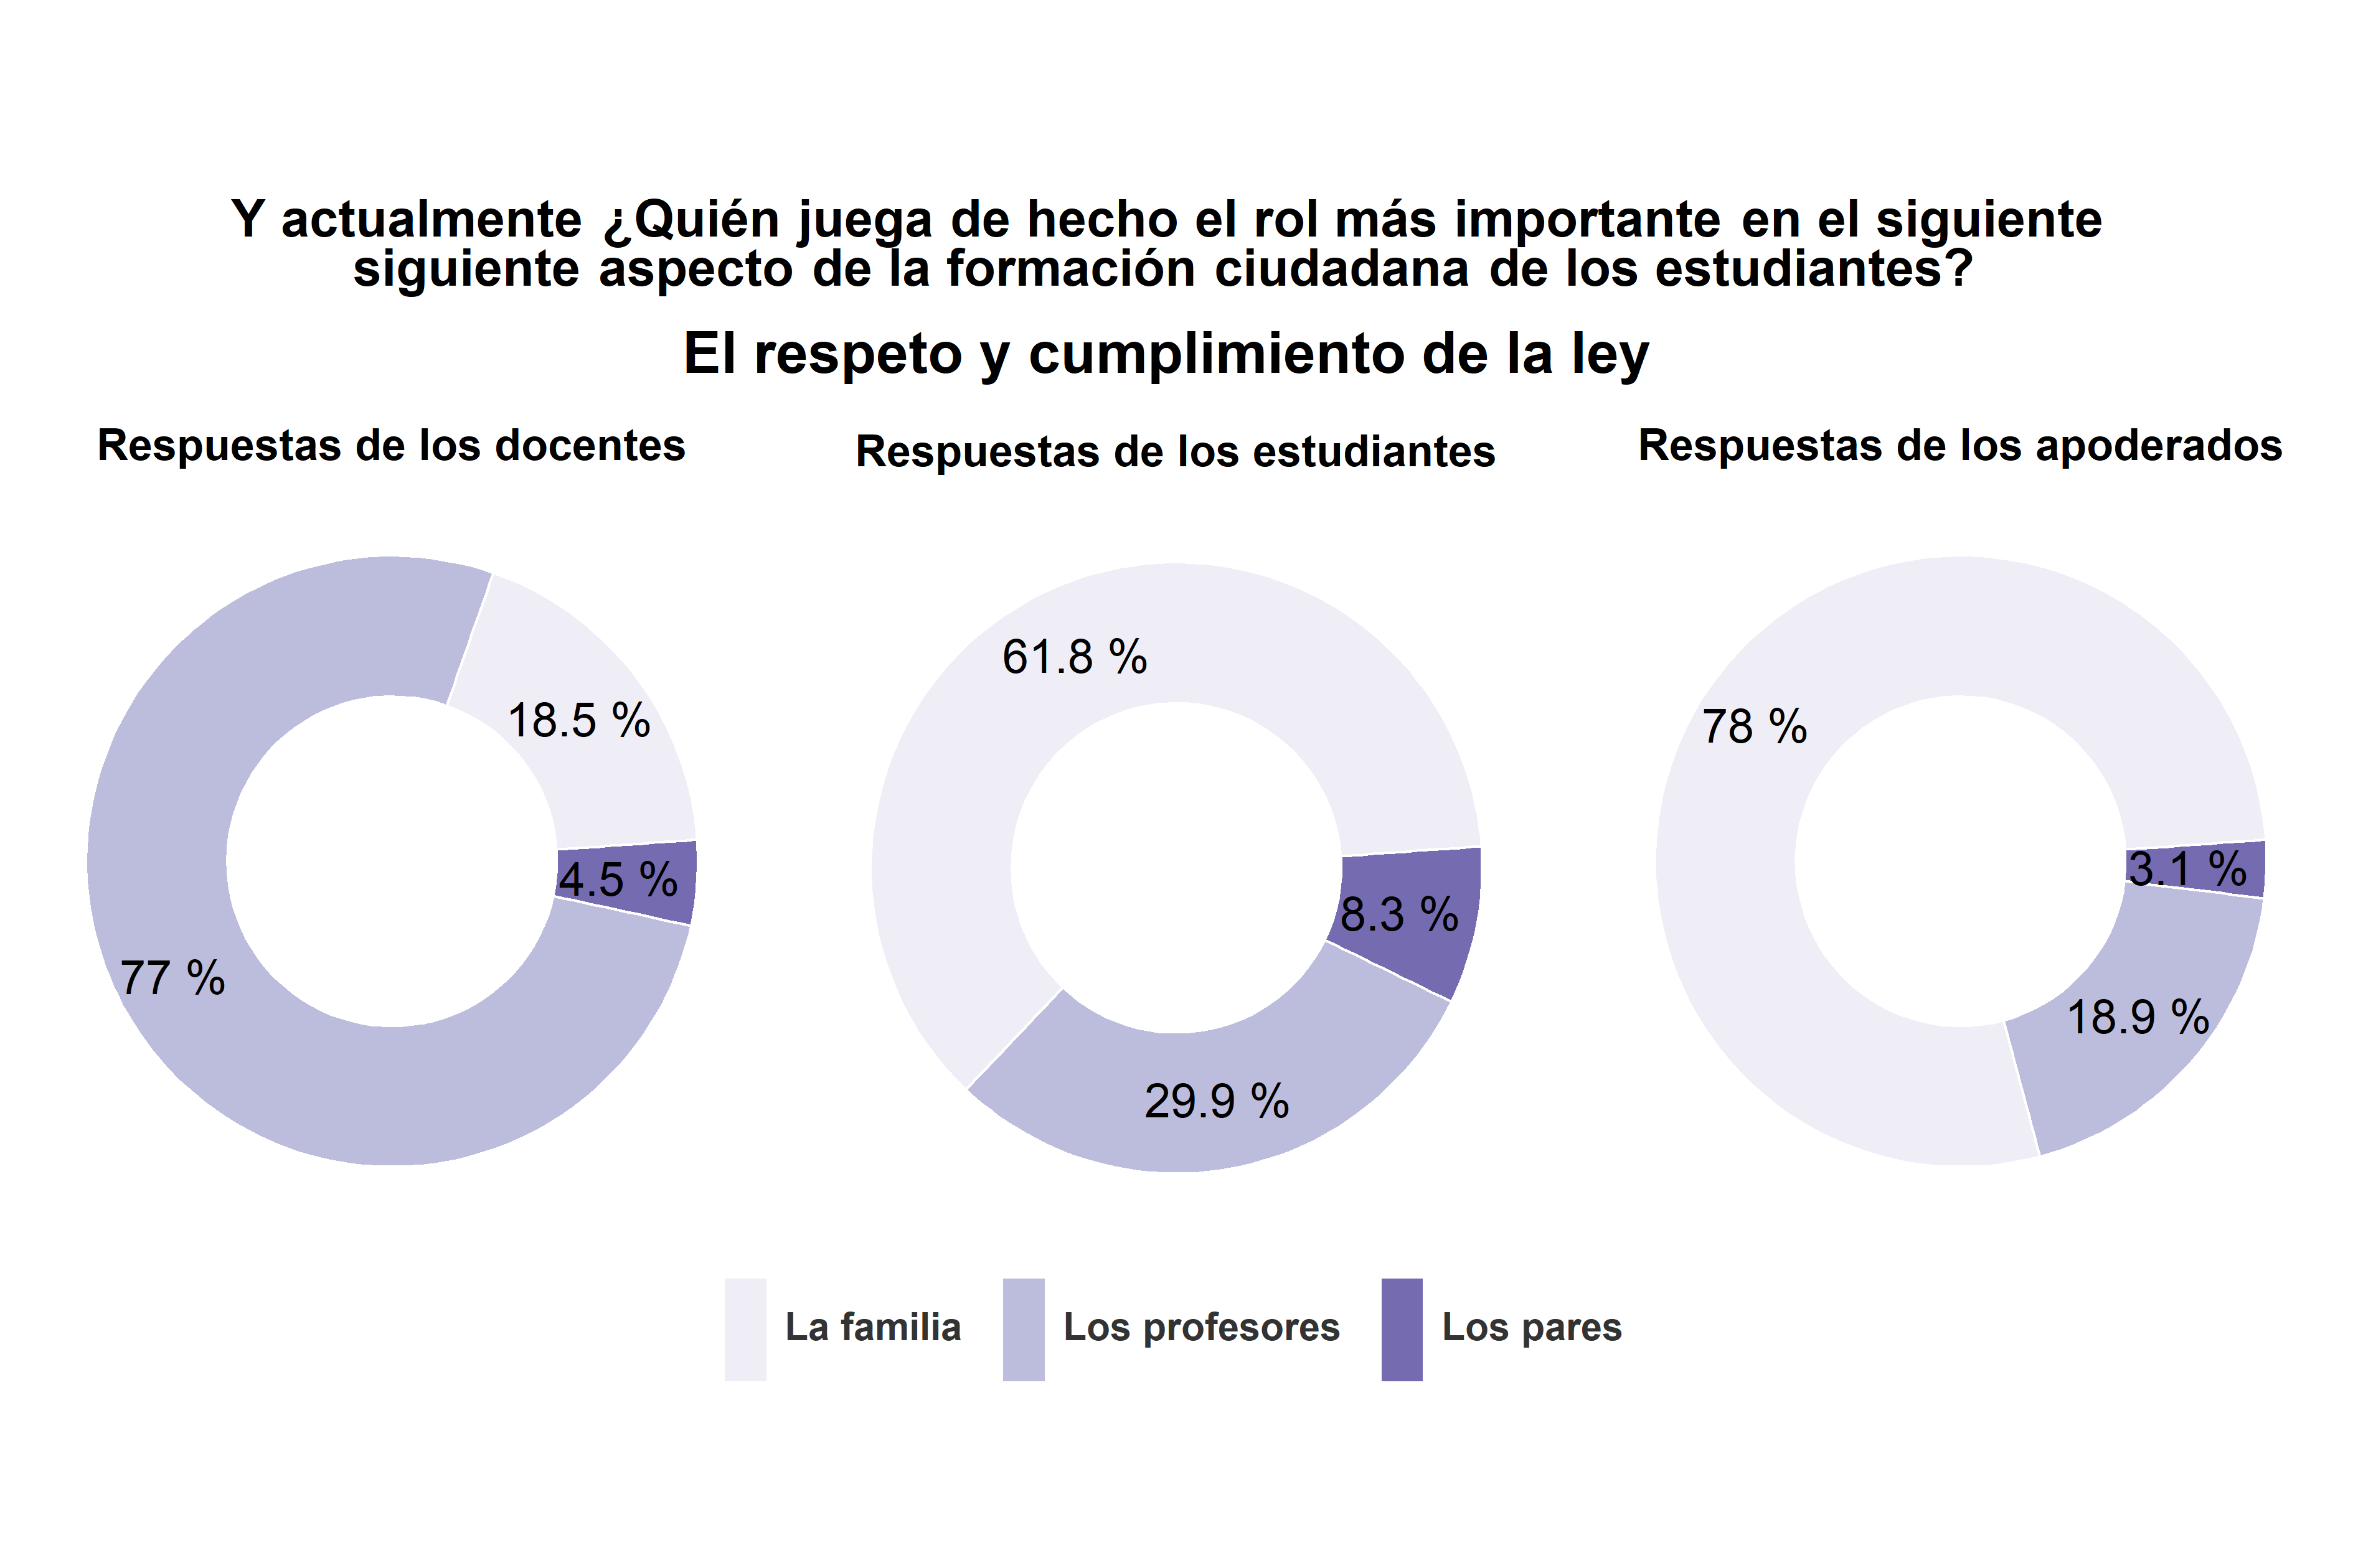
\includegraphics[width=52.49in]{images/graph_for_ciud11} \end{center}

\hypertarget{actitudes-poluxedticas}{%
\chapter{Actitudes políticas}\label{actitudes-poluxedticas}}

\hypertarget{secciuxf3n-1-interuxe9s-en-poluxedtica-y-problemas-sociales}{%
\section{Sección 1: Interés en política y problemas sociales}\label{secciuxf3n-1-interuxe9s-en-poluxedtica-y-problemas-sociales}}

\begin{center}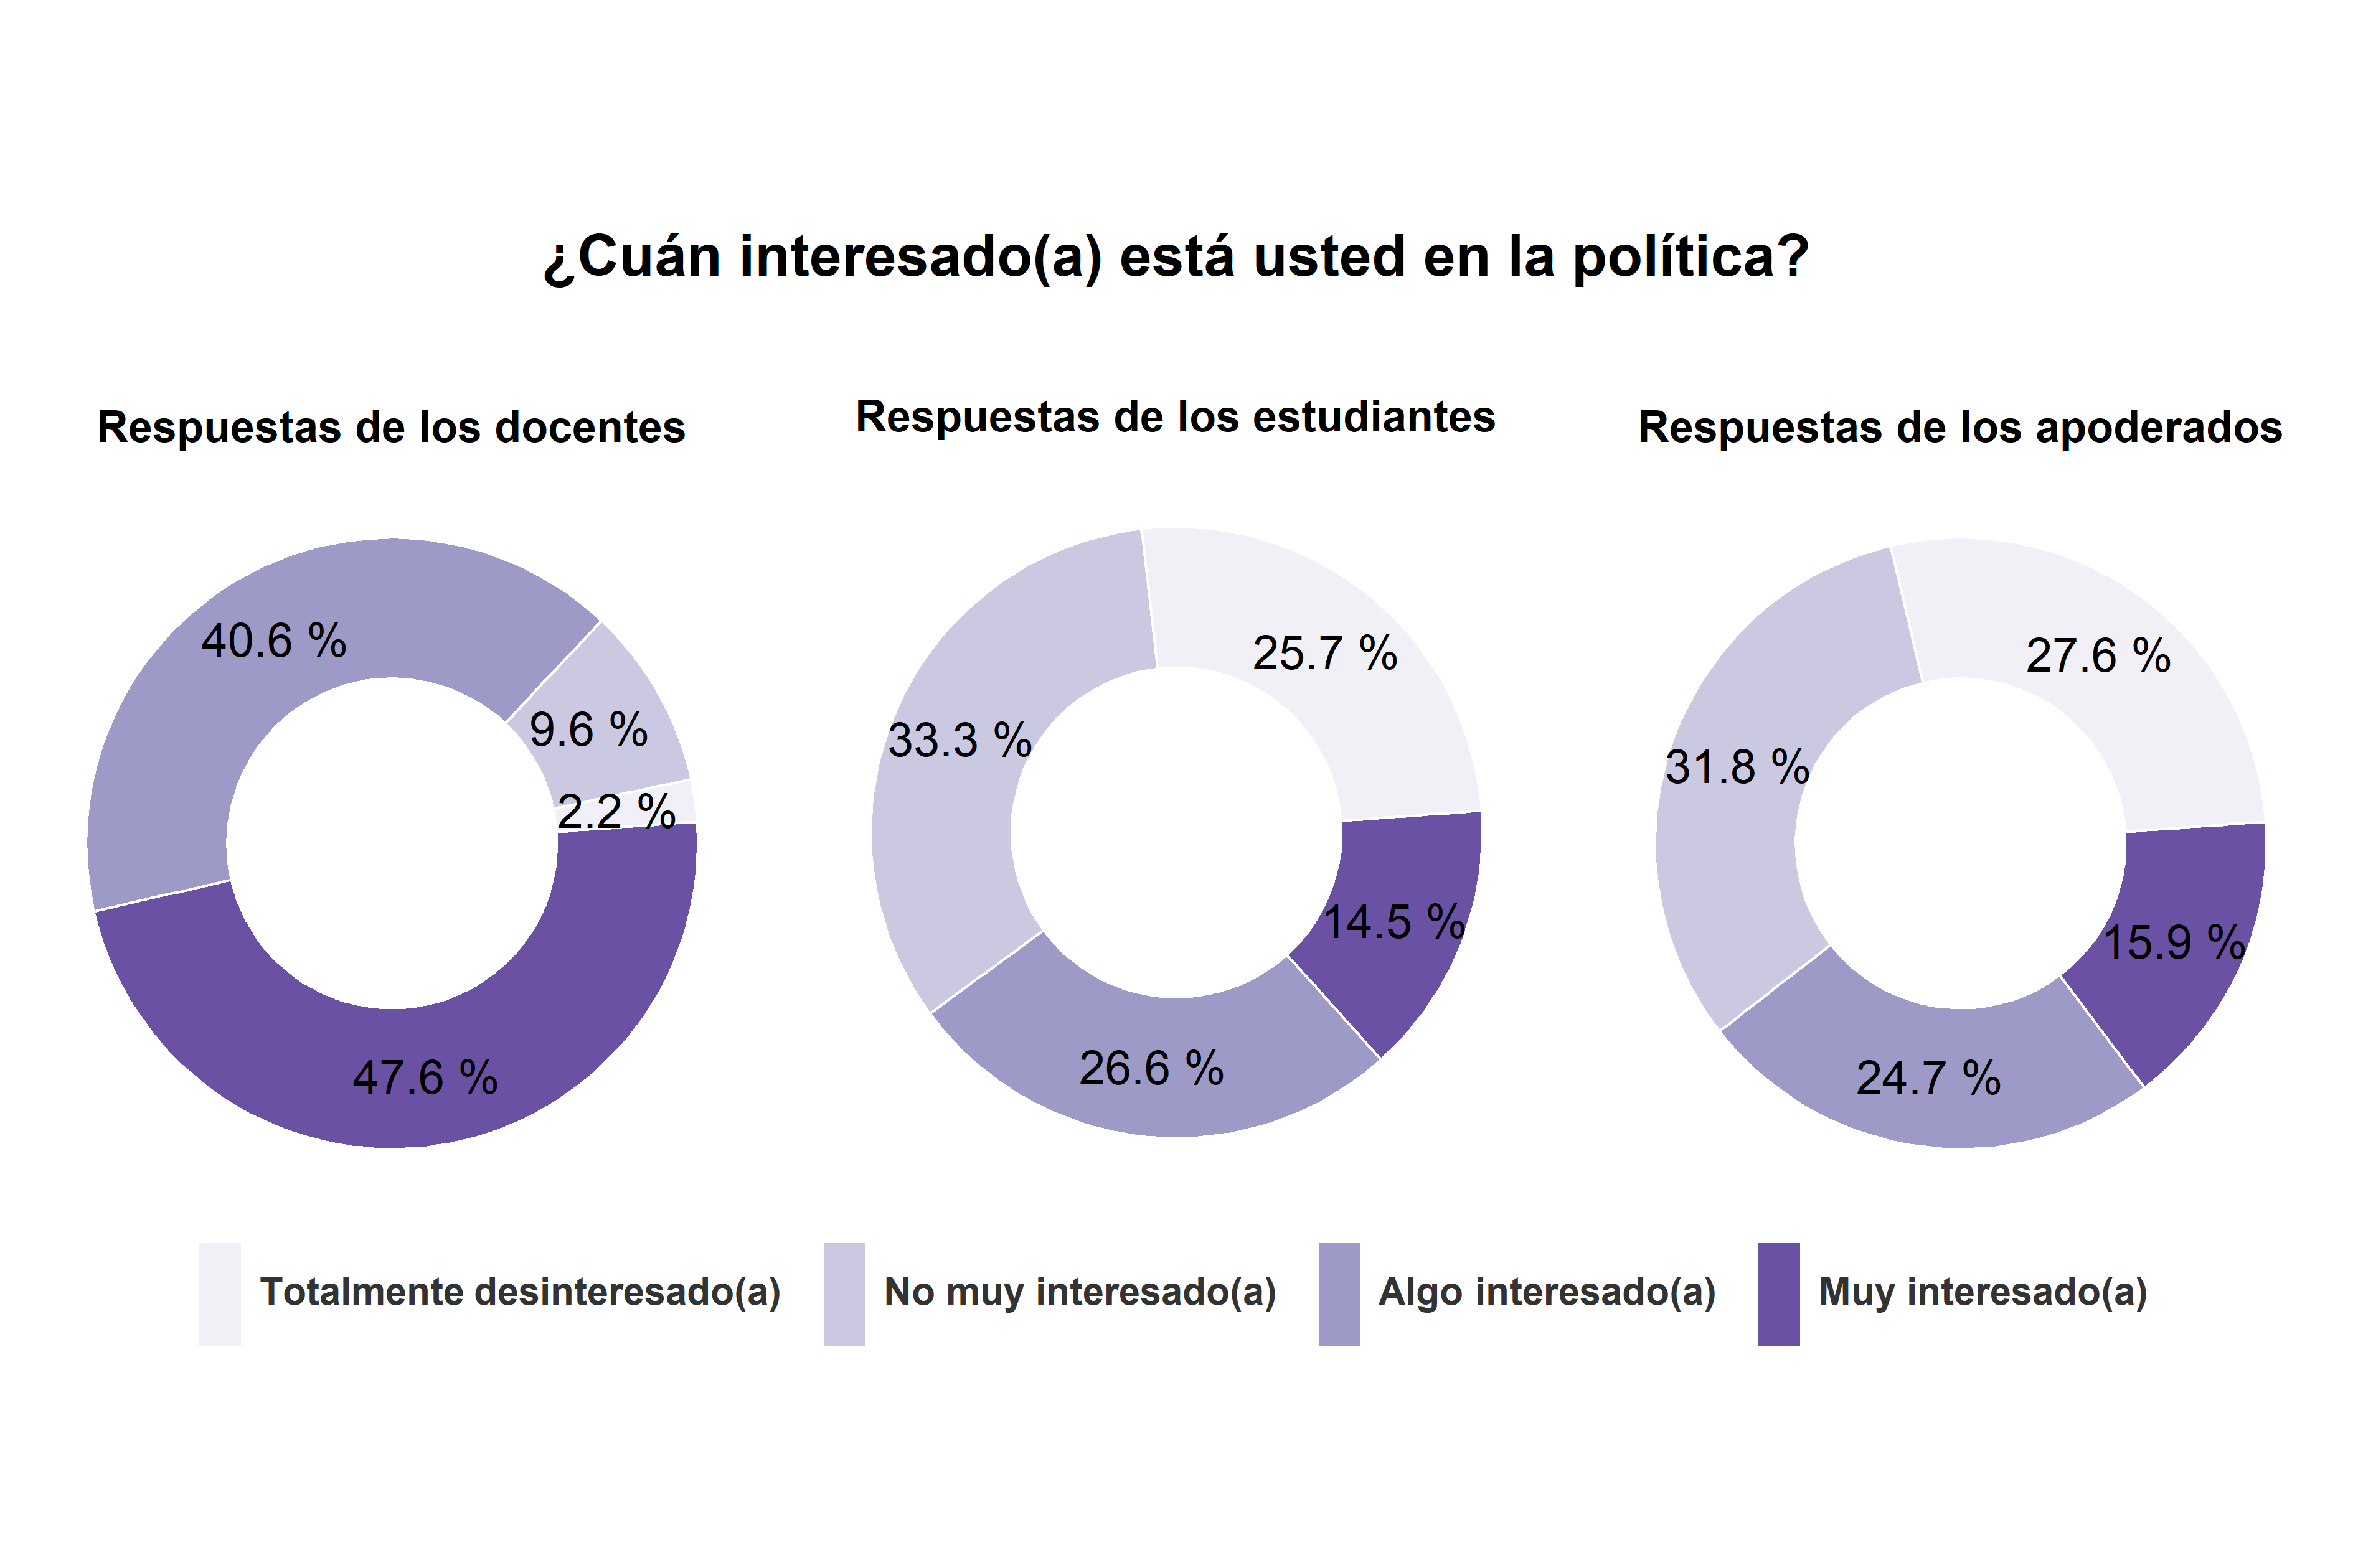
\includegraphics[width=52.49in]{images/graph_intpol} \end{center}

\begin{center}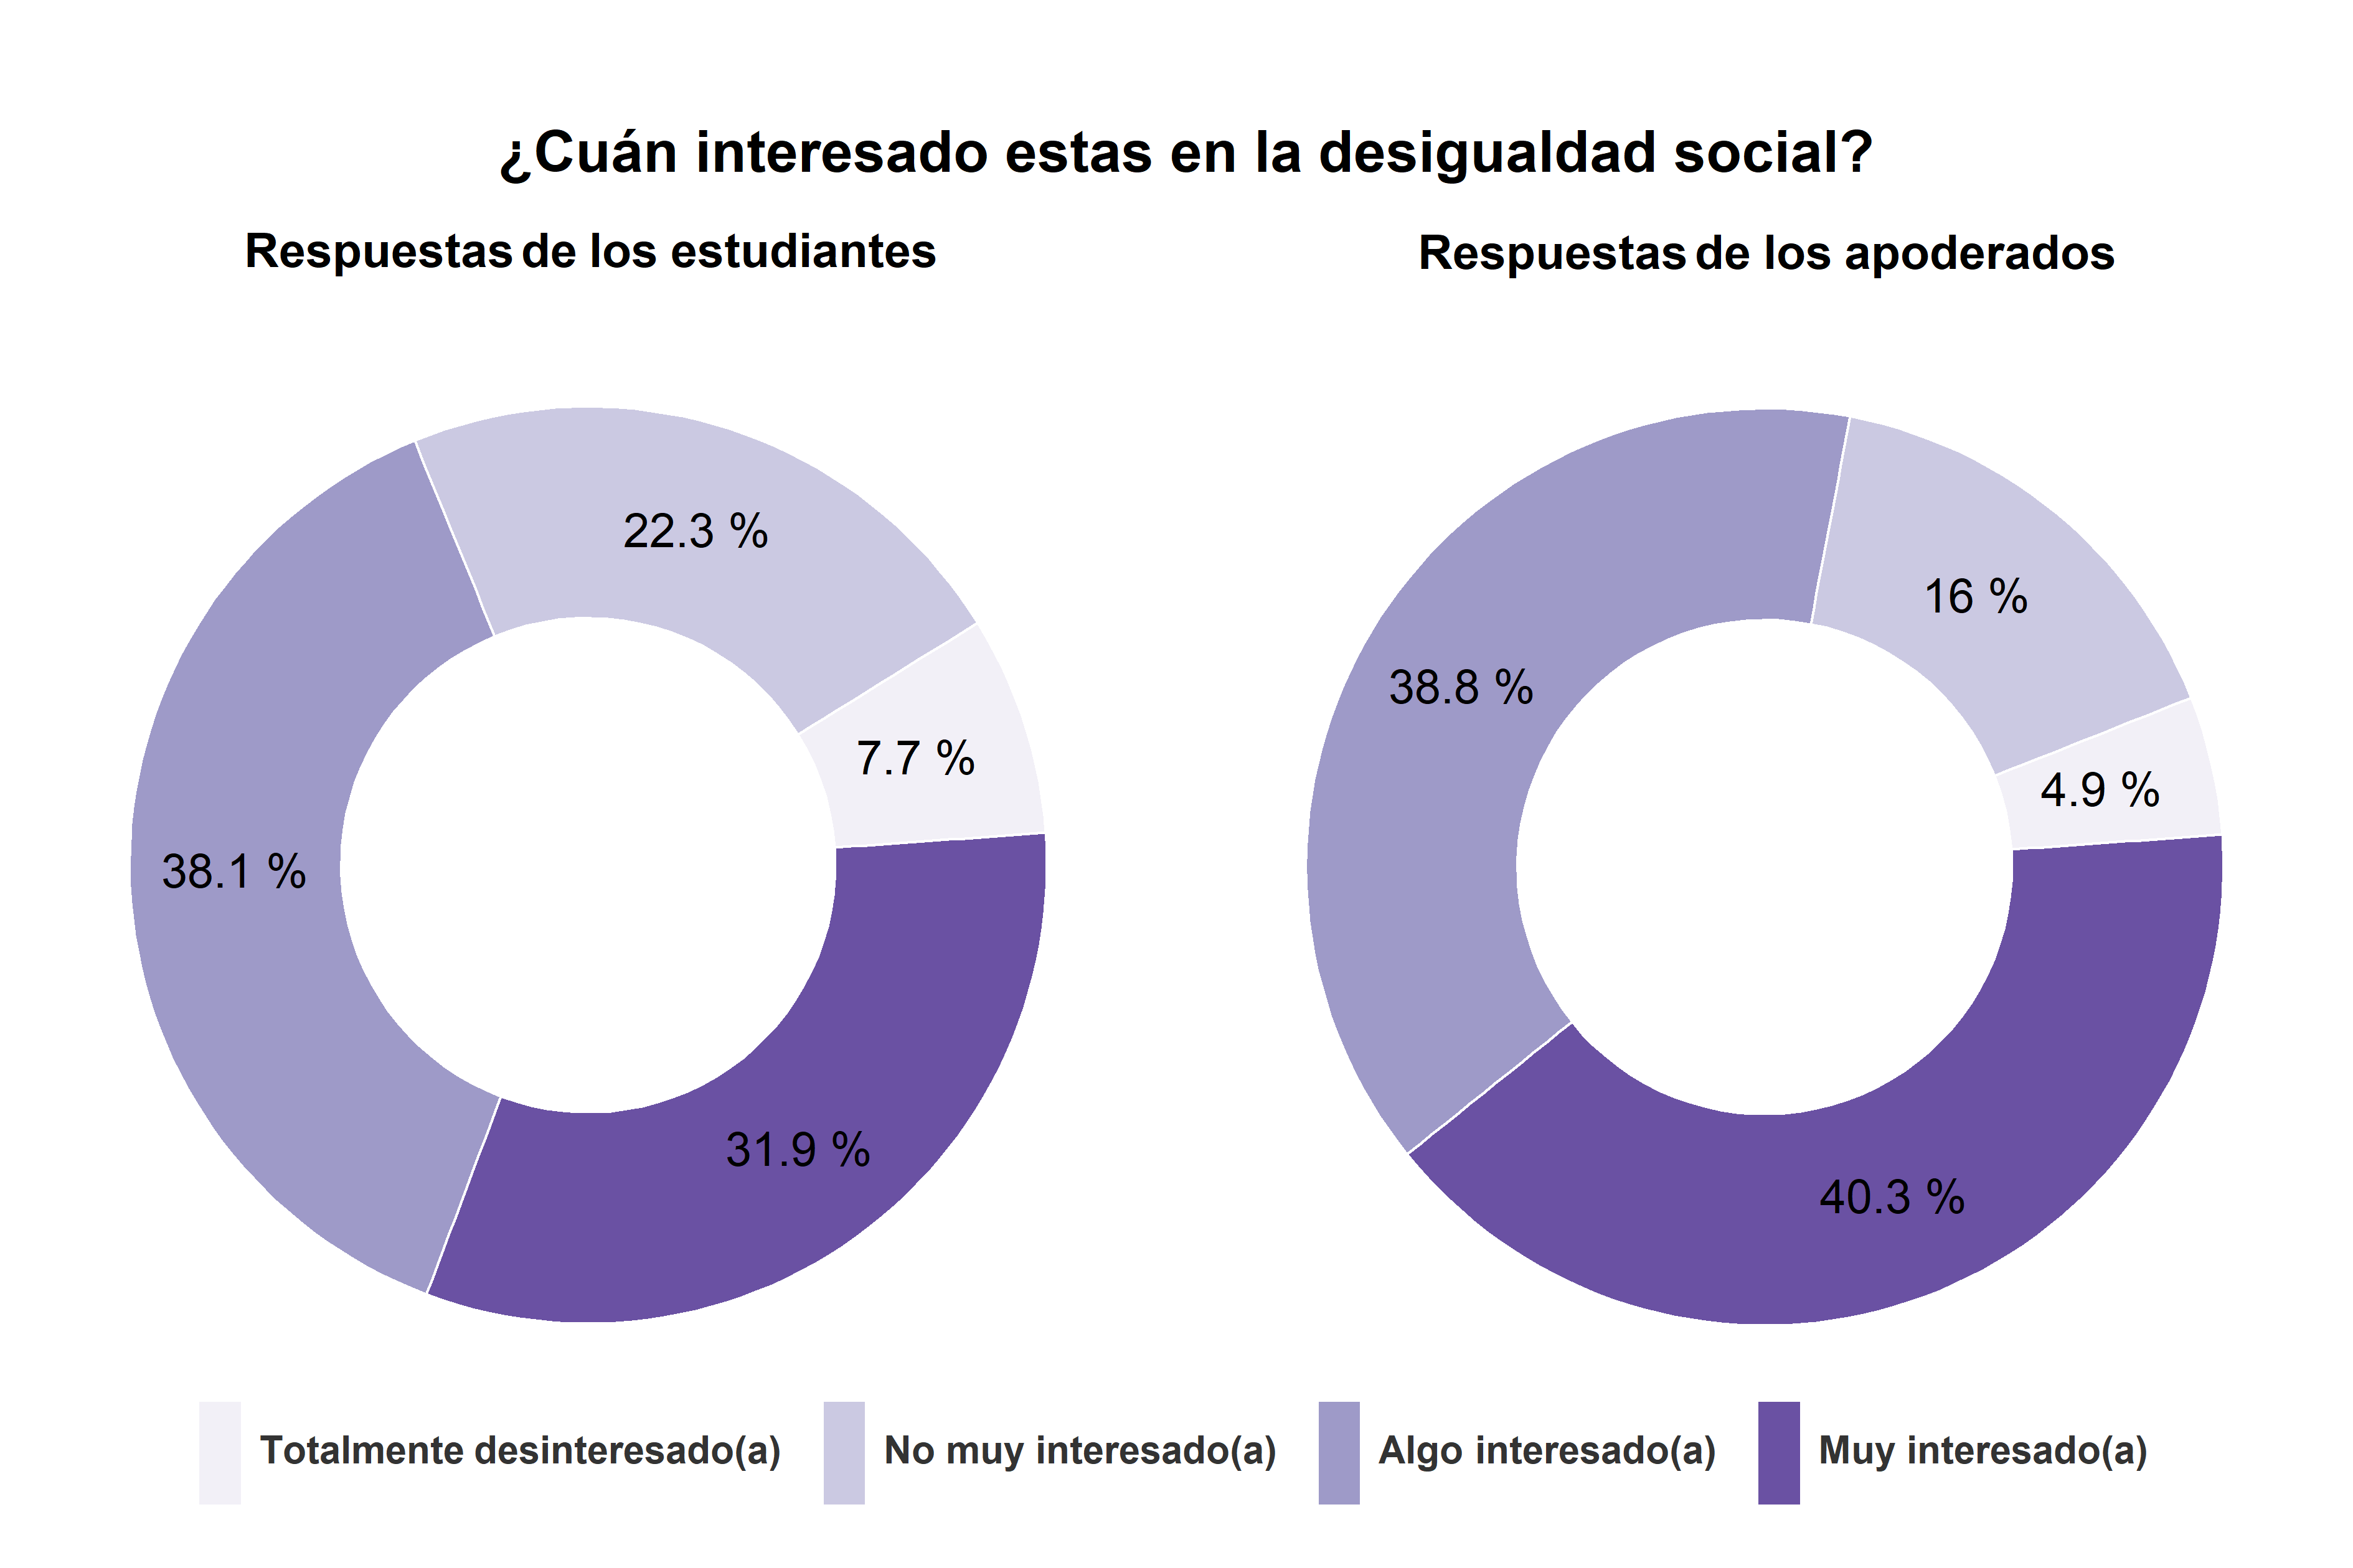
\includegraphics[width=52.49in]{images/graph_intdes} \end{center}

\begin{center}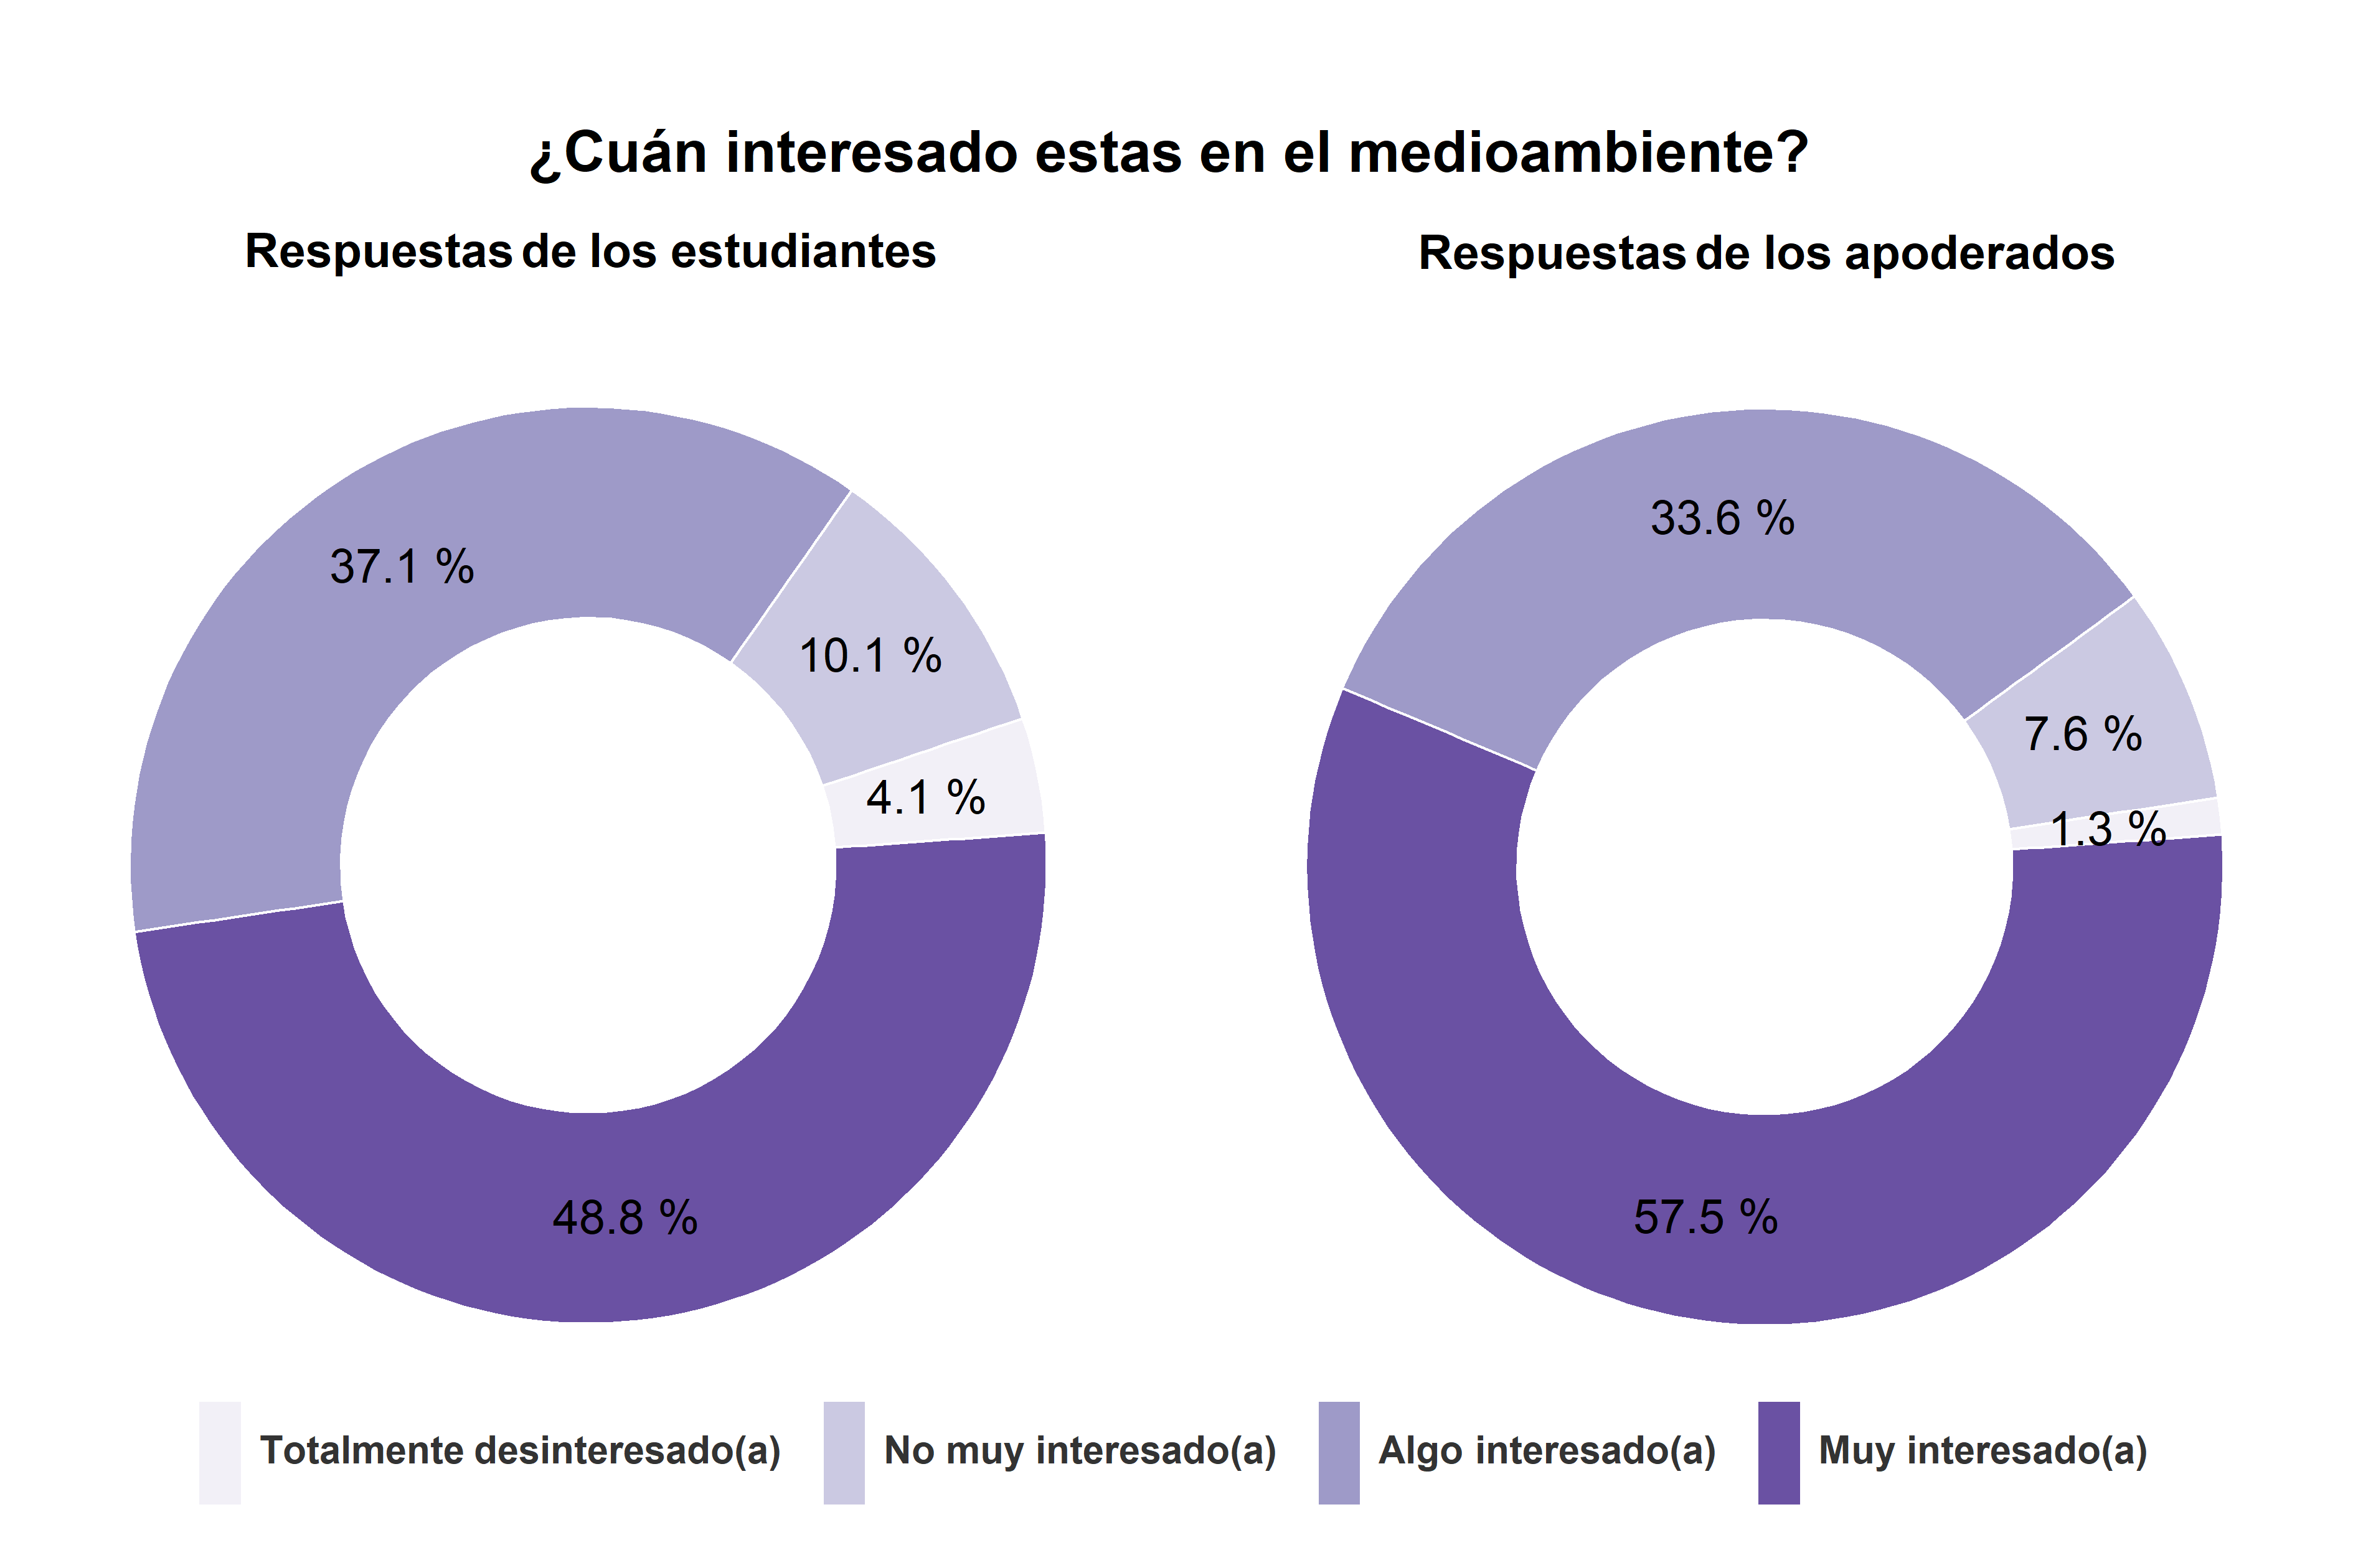
\includegraphics[width=52.49in]{images/graph_intmed} \end{center}

\begin{center}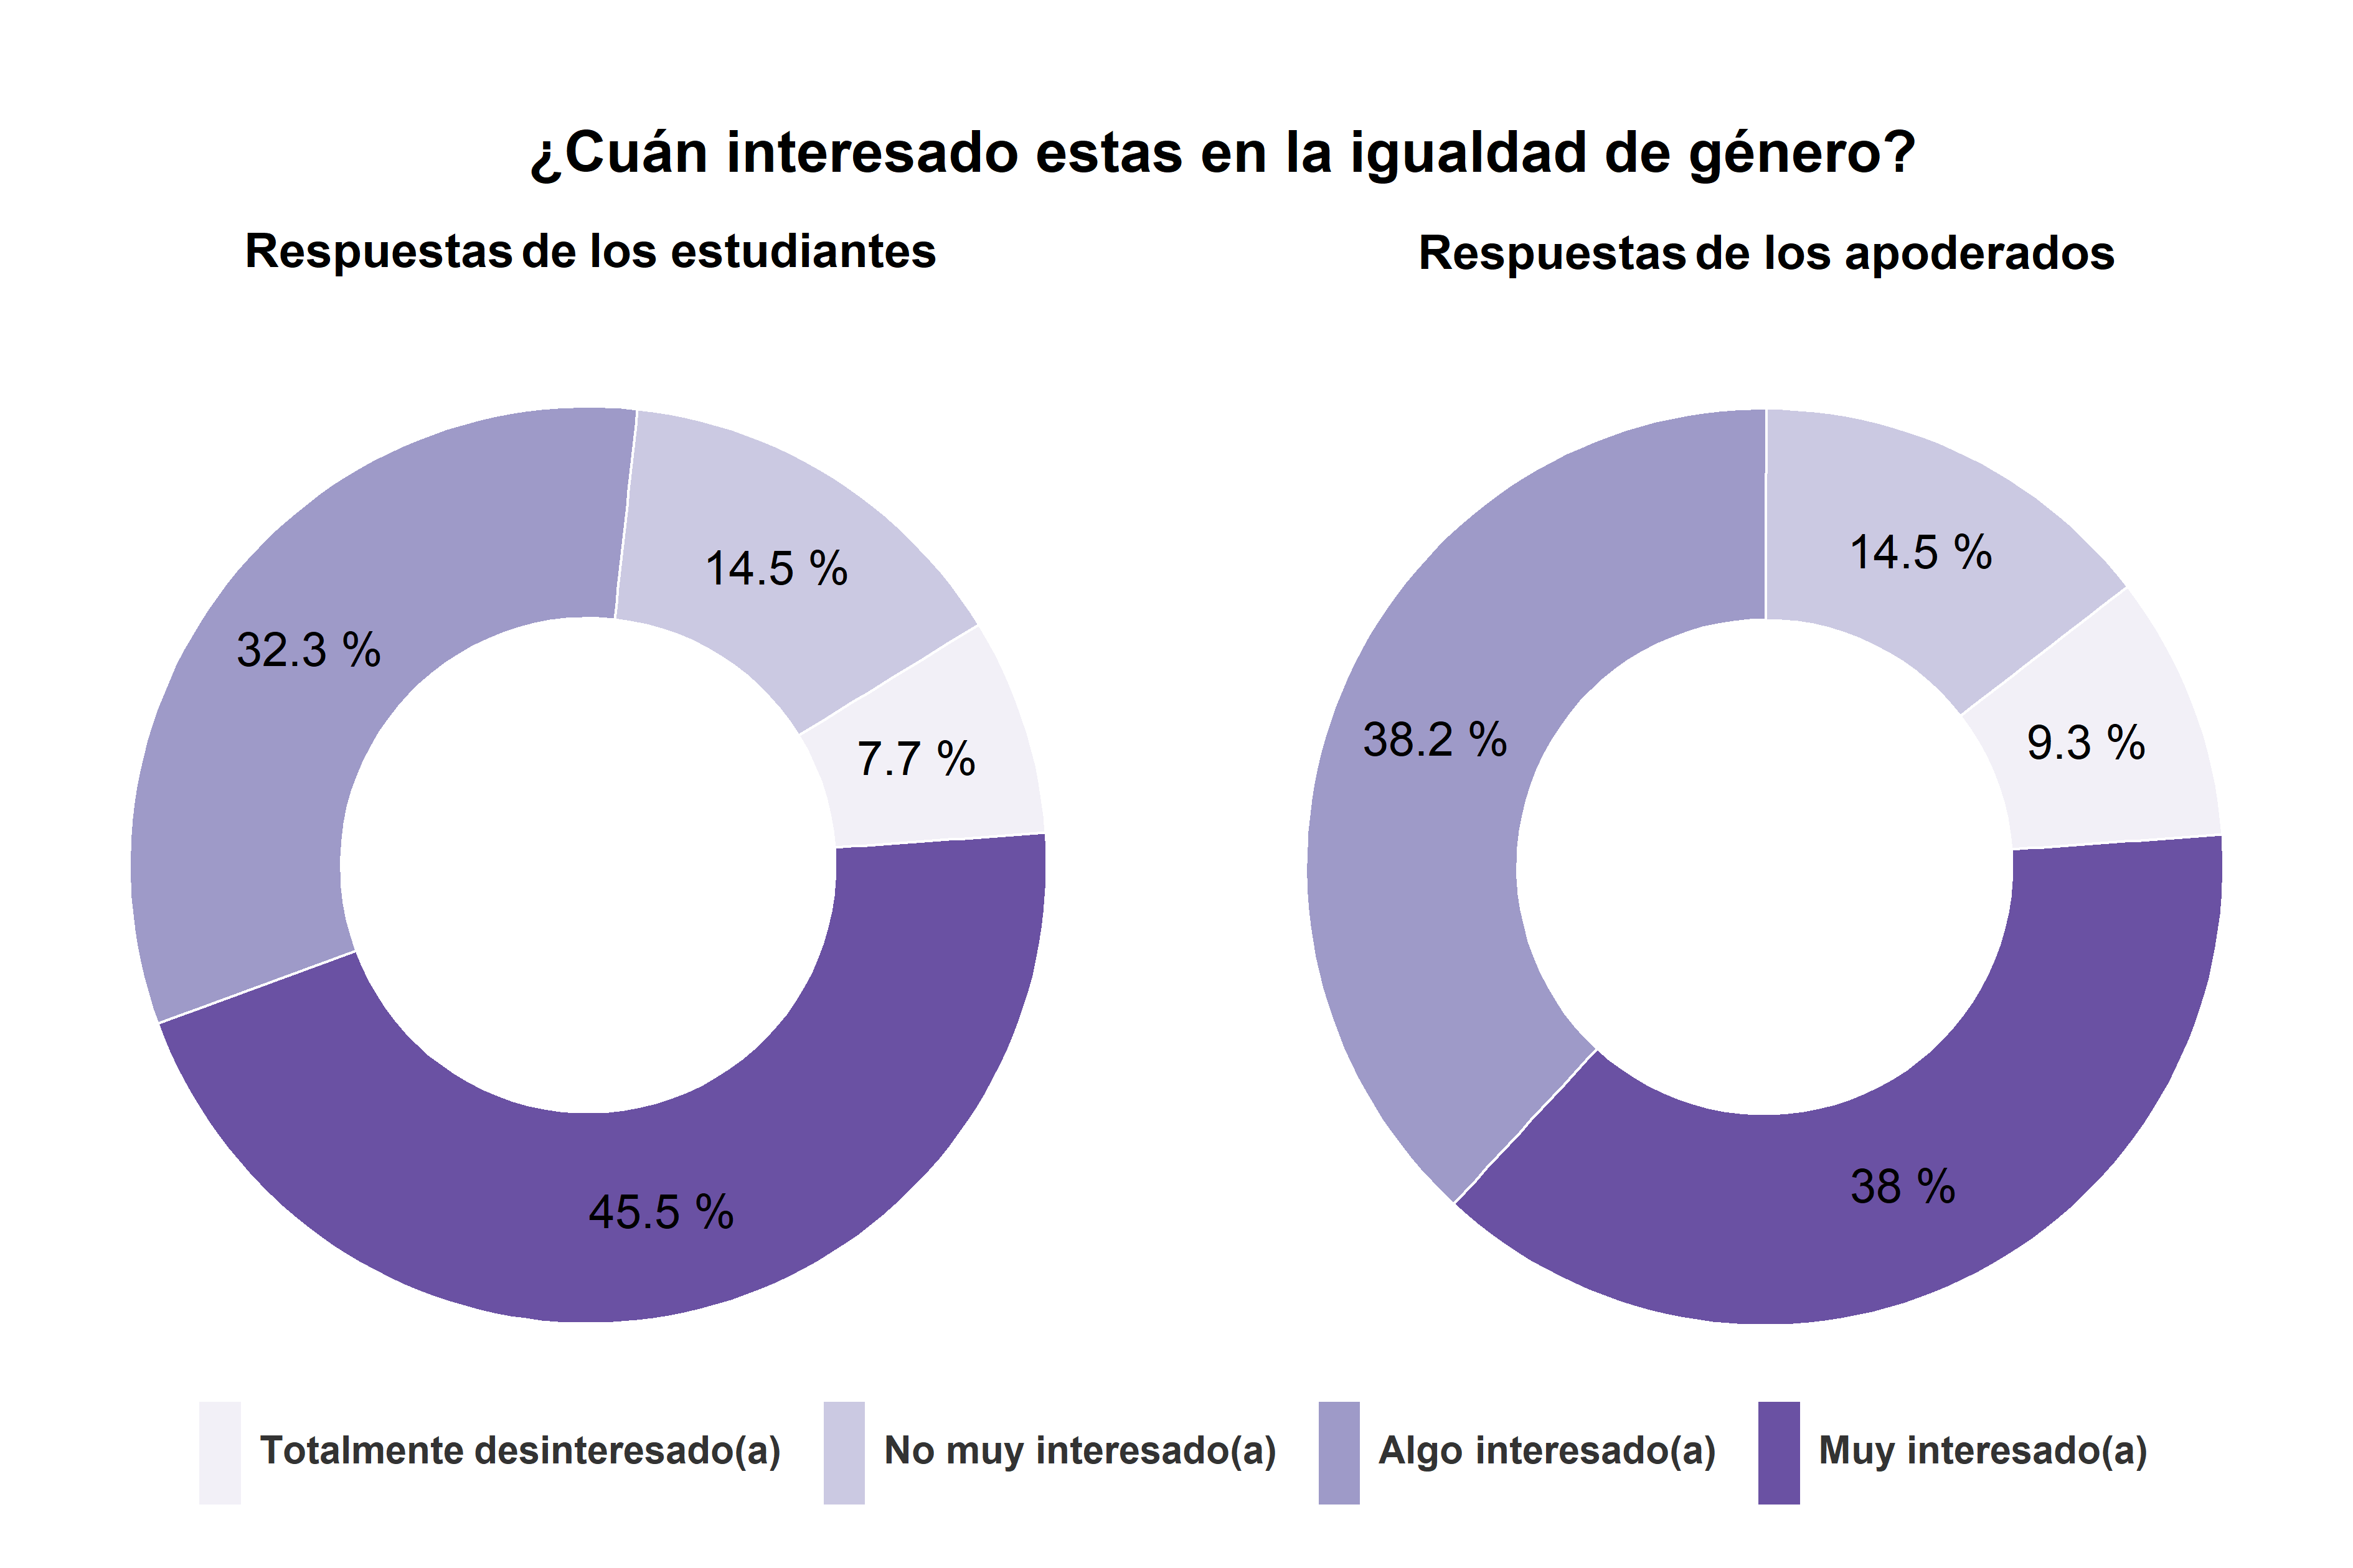
\includegraphics[width=52.49in]{images/graph_intgen} \end{center}

\hypertarget{secciuxf3n-2-satisfacciuxf3n-con-la-democracia-y-actitudes-autoritarias}{%
\section{Sección 2: Satisfacción con la democracia y actitudes autoritarias}\label{secciuxf3n-2-satisfacciuxf3n-con-la-democracia-y-actitudes-autoritarias}}

\begin{center}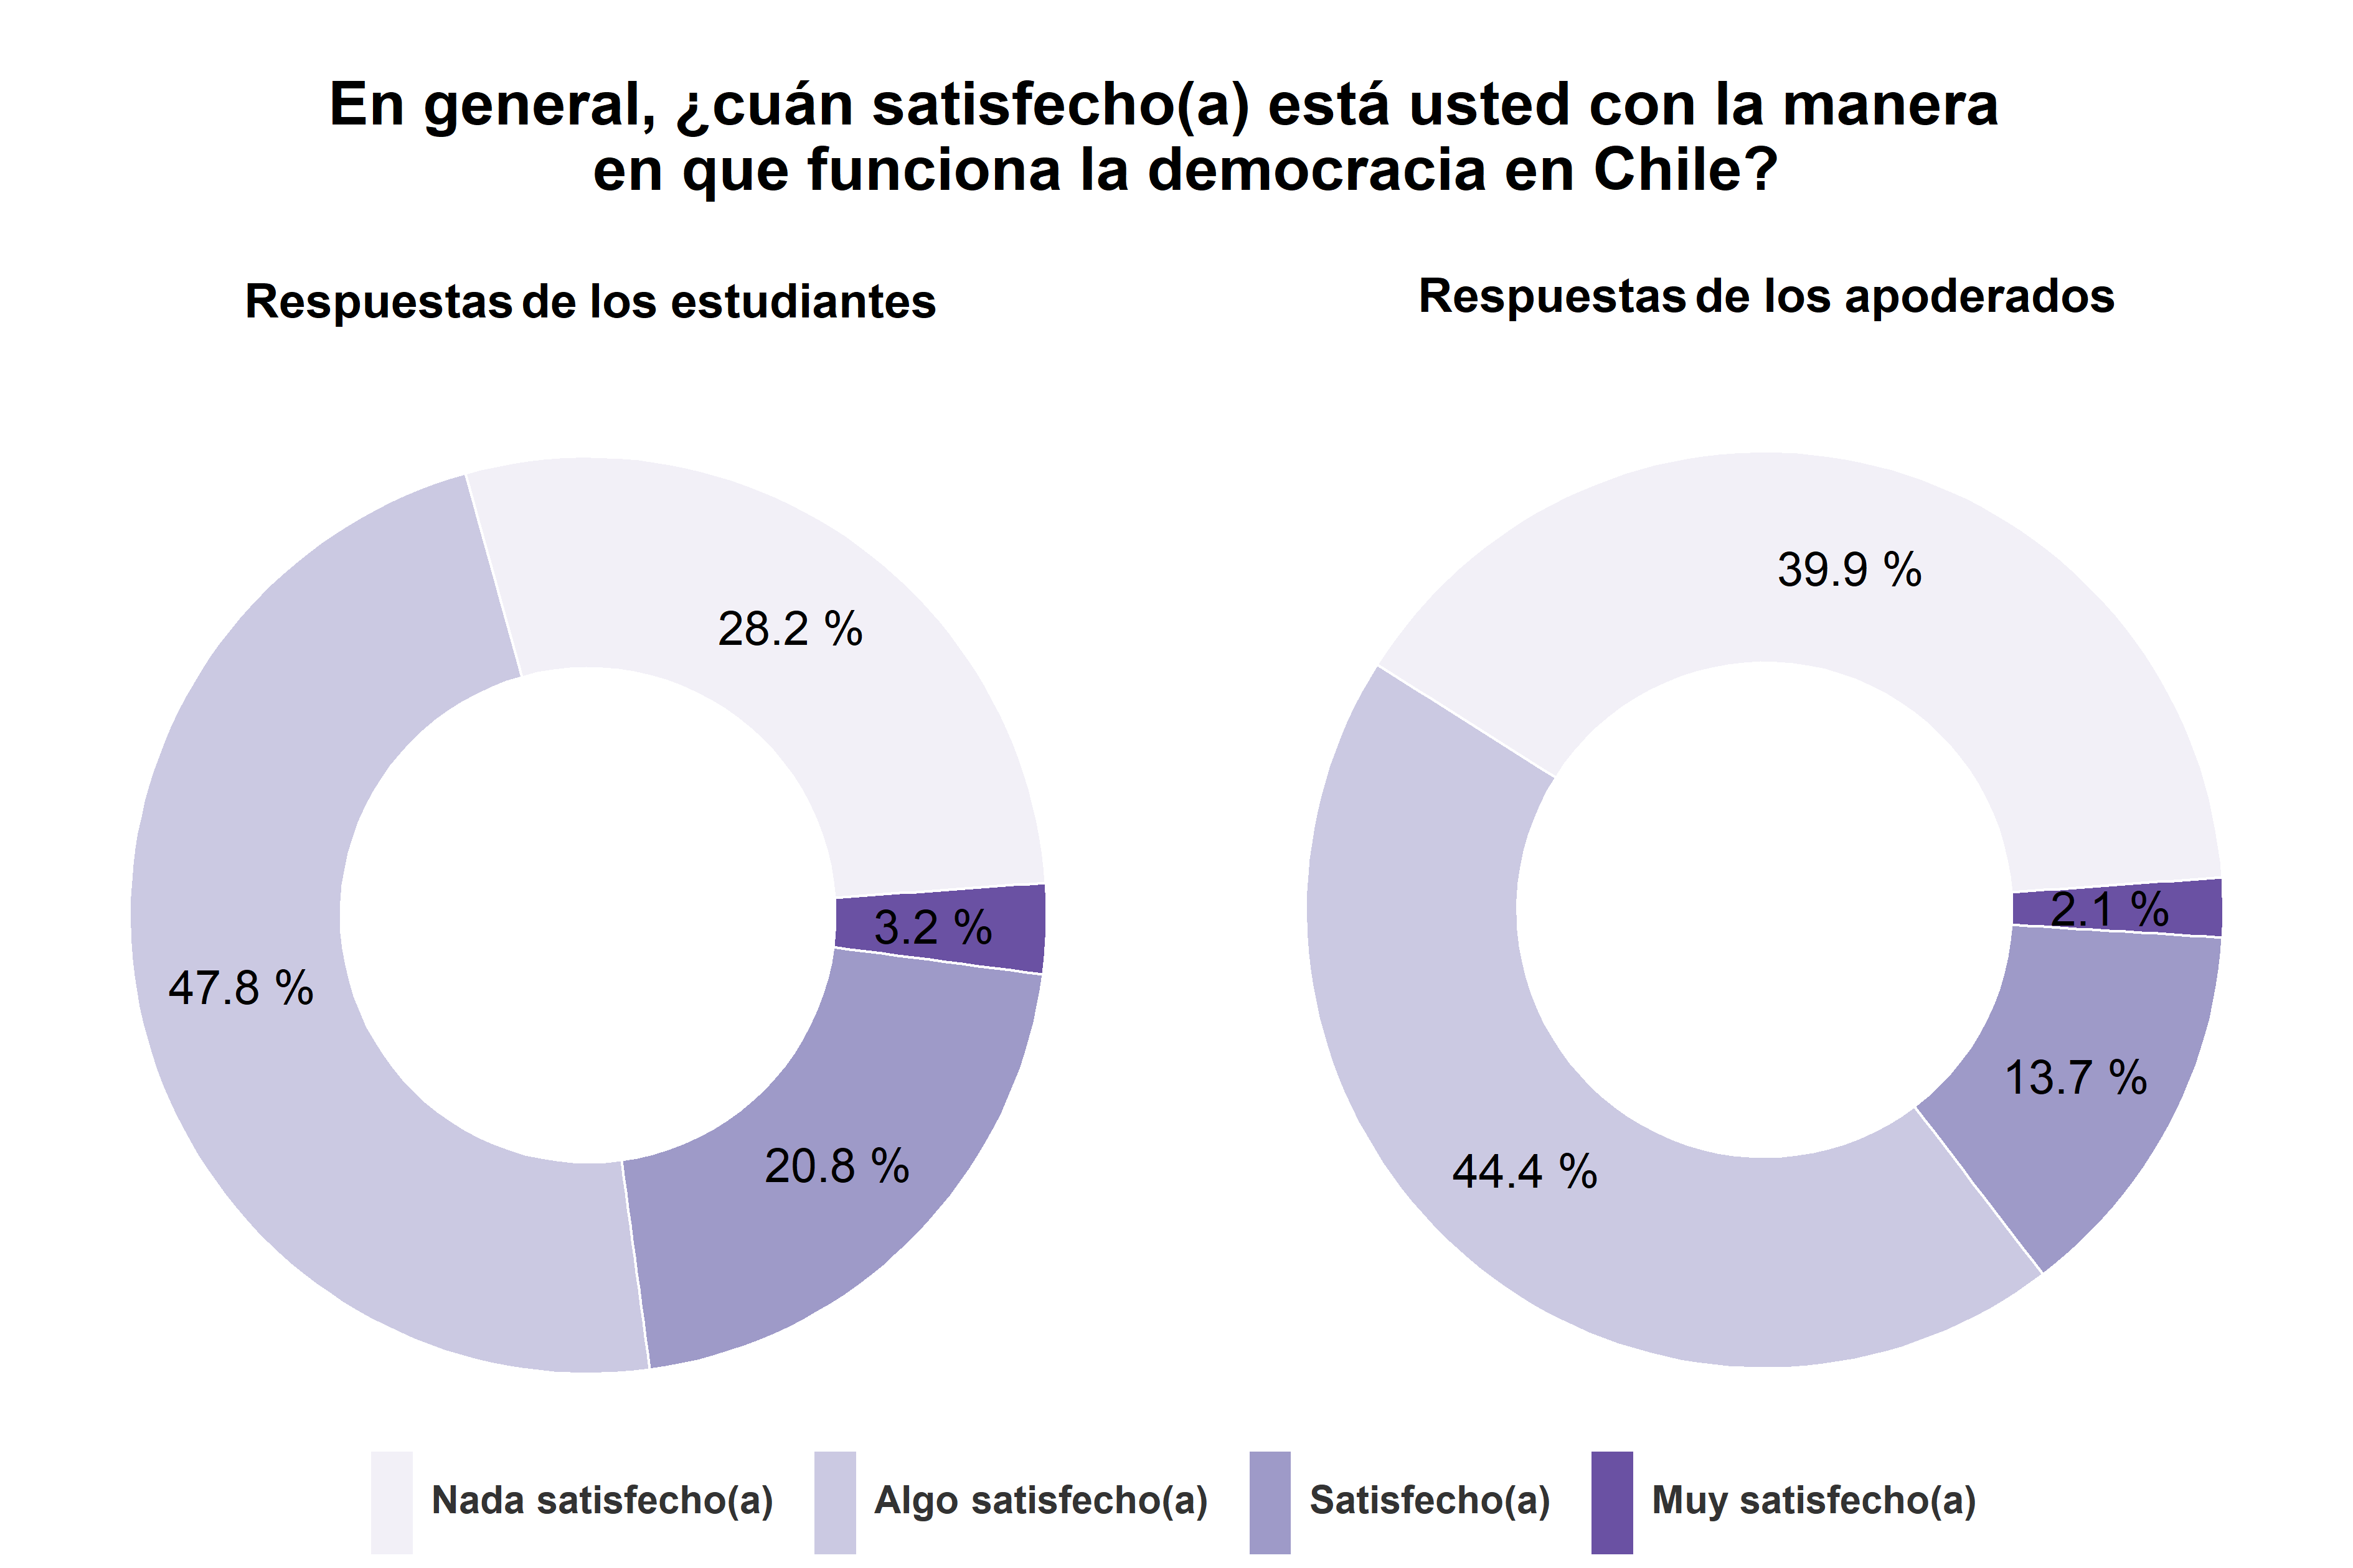
\includegraphics[width=52.49in]{images/graph_dem} \end{center}

\begin{center}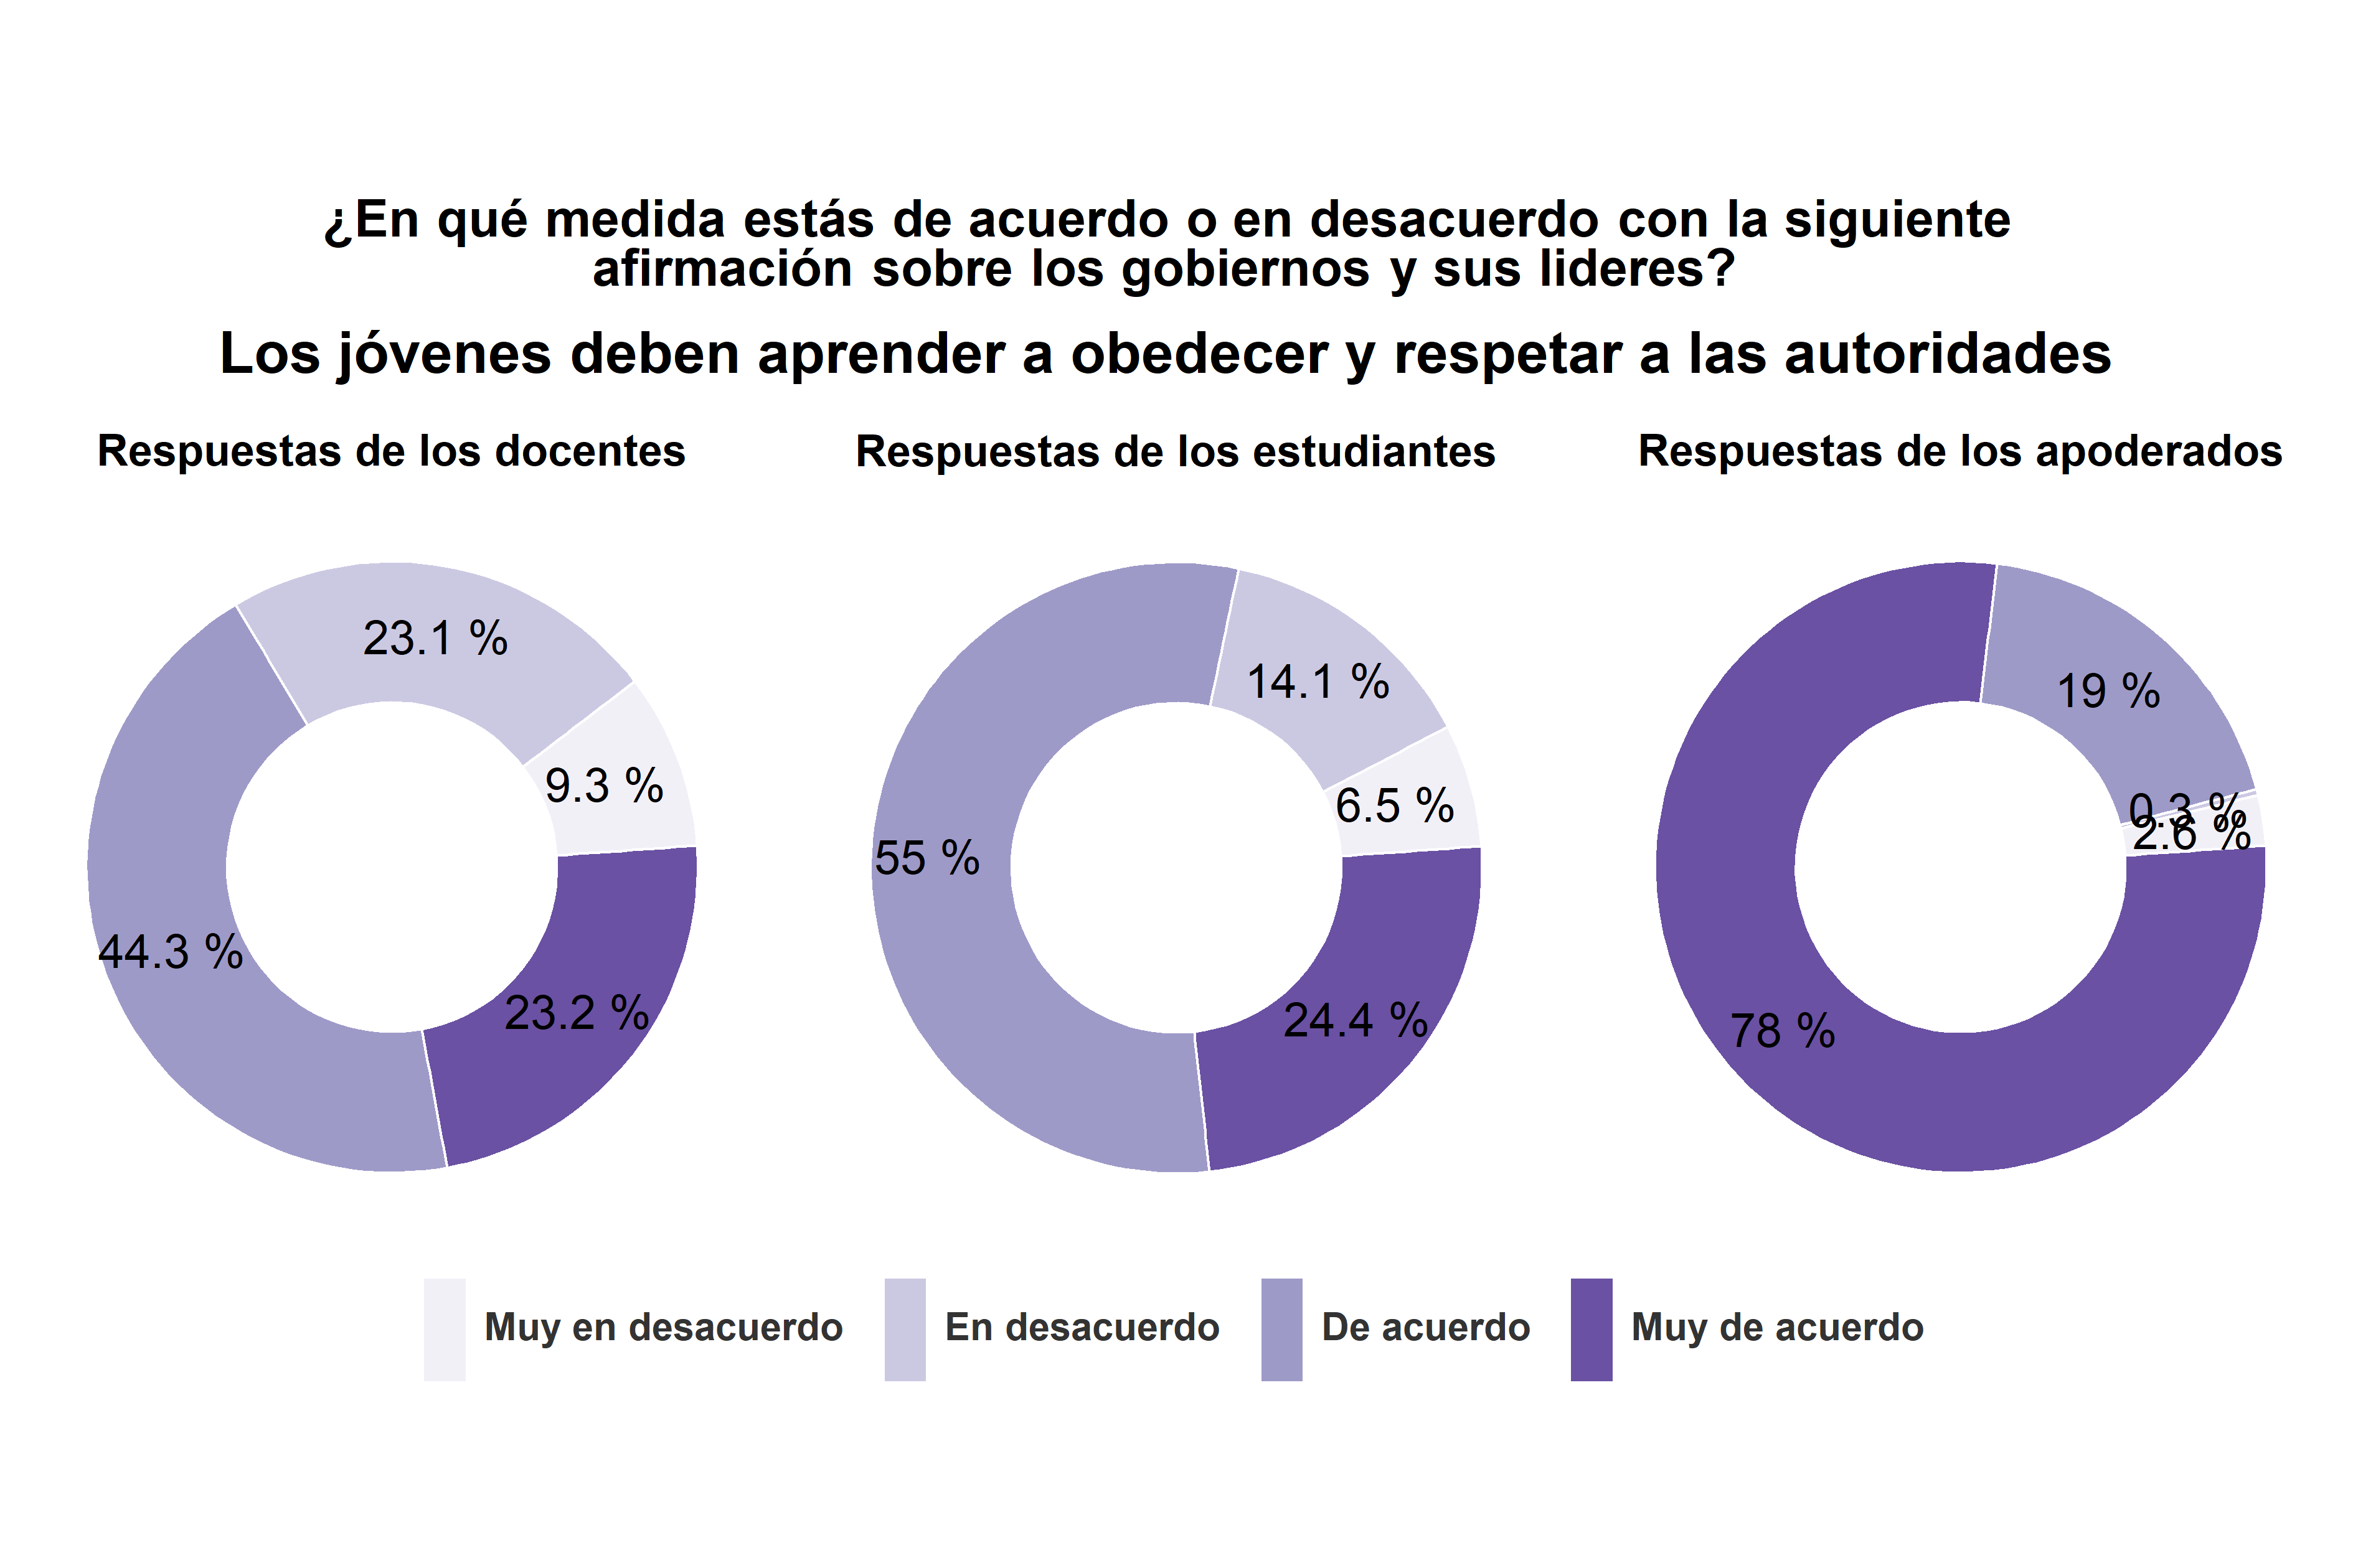
\includegraphics[width=52.49in]{images/graph_aut1} \end{center}

\begin{center}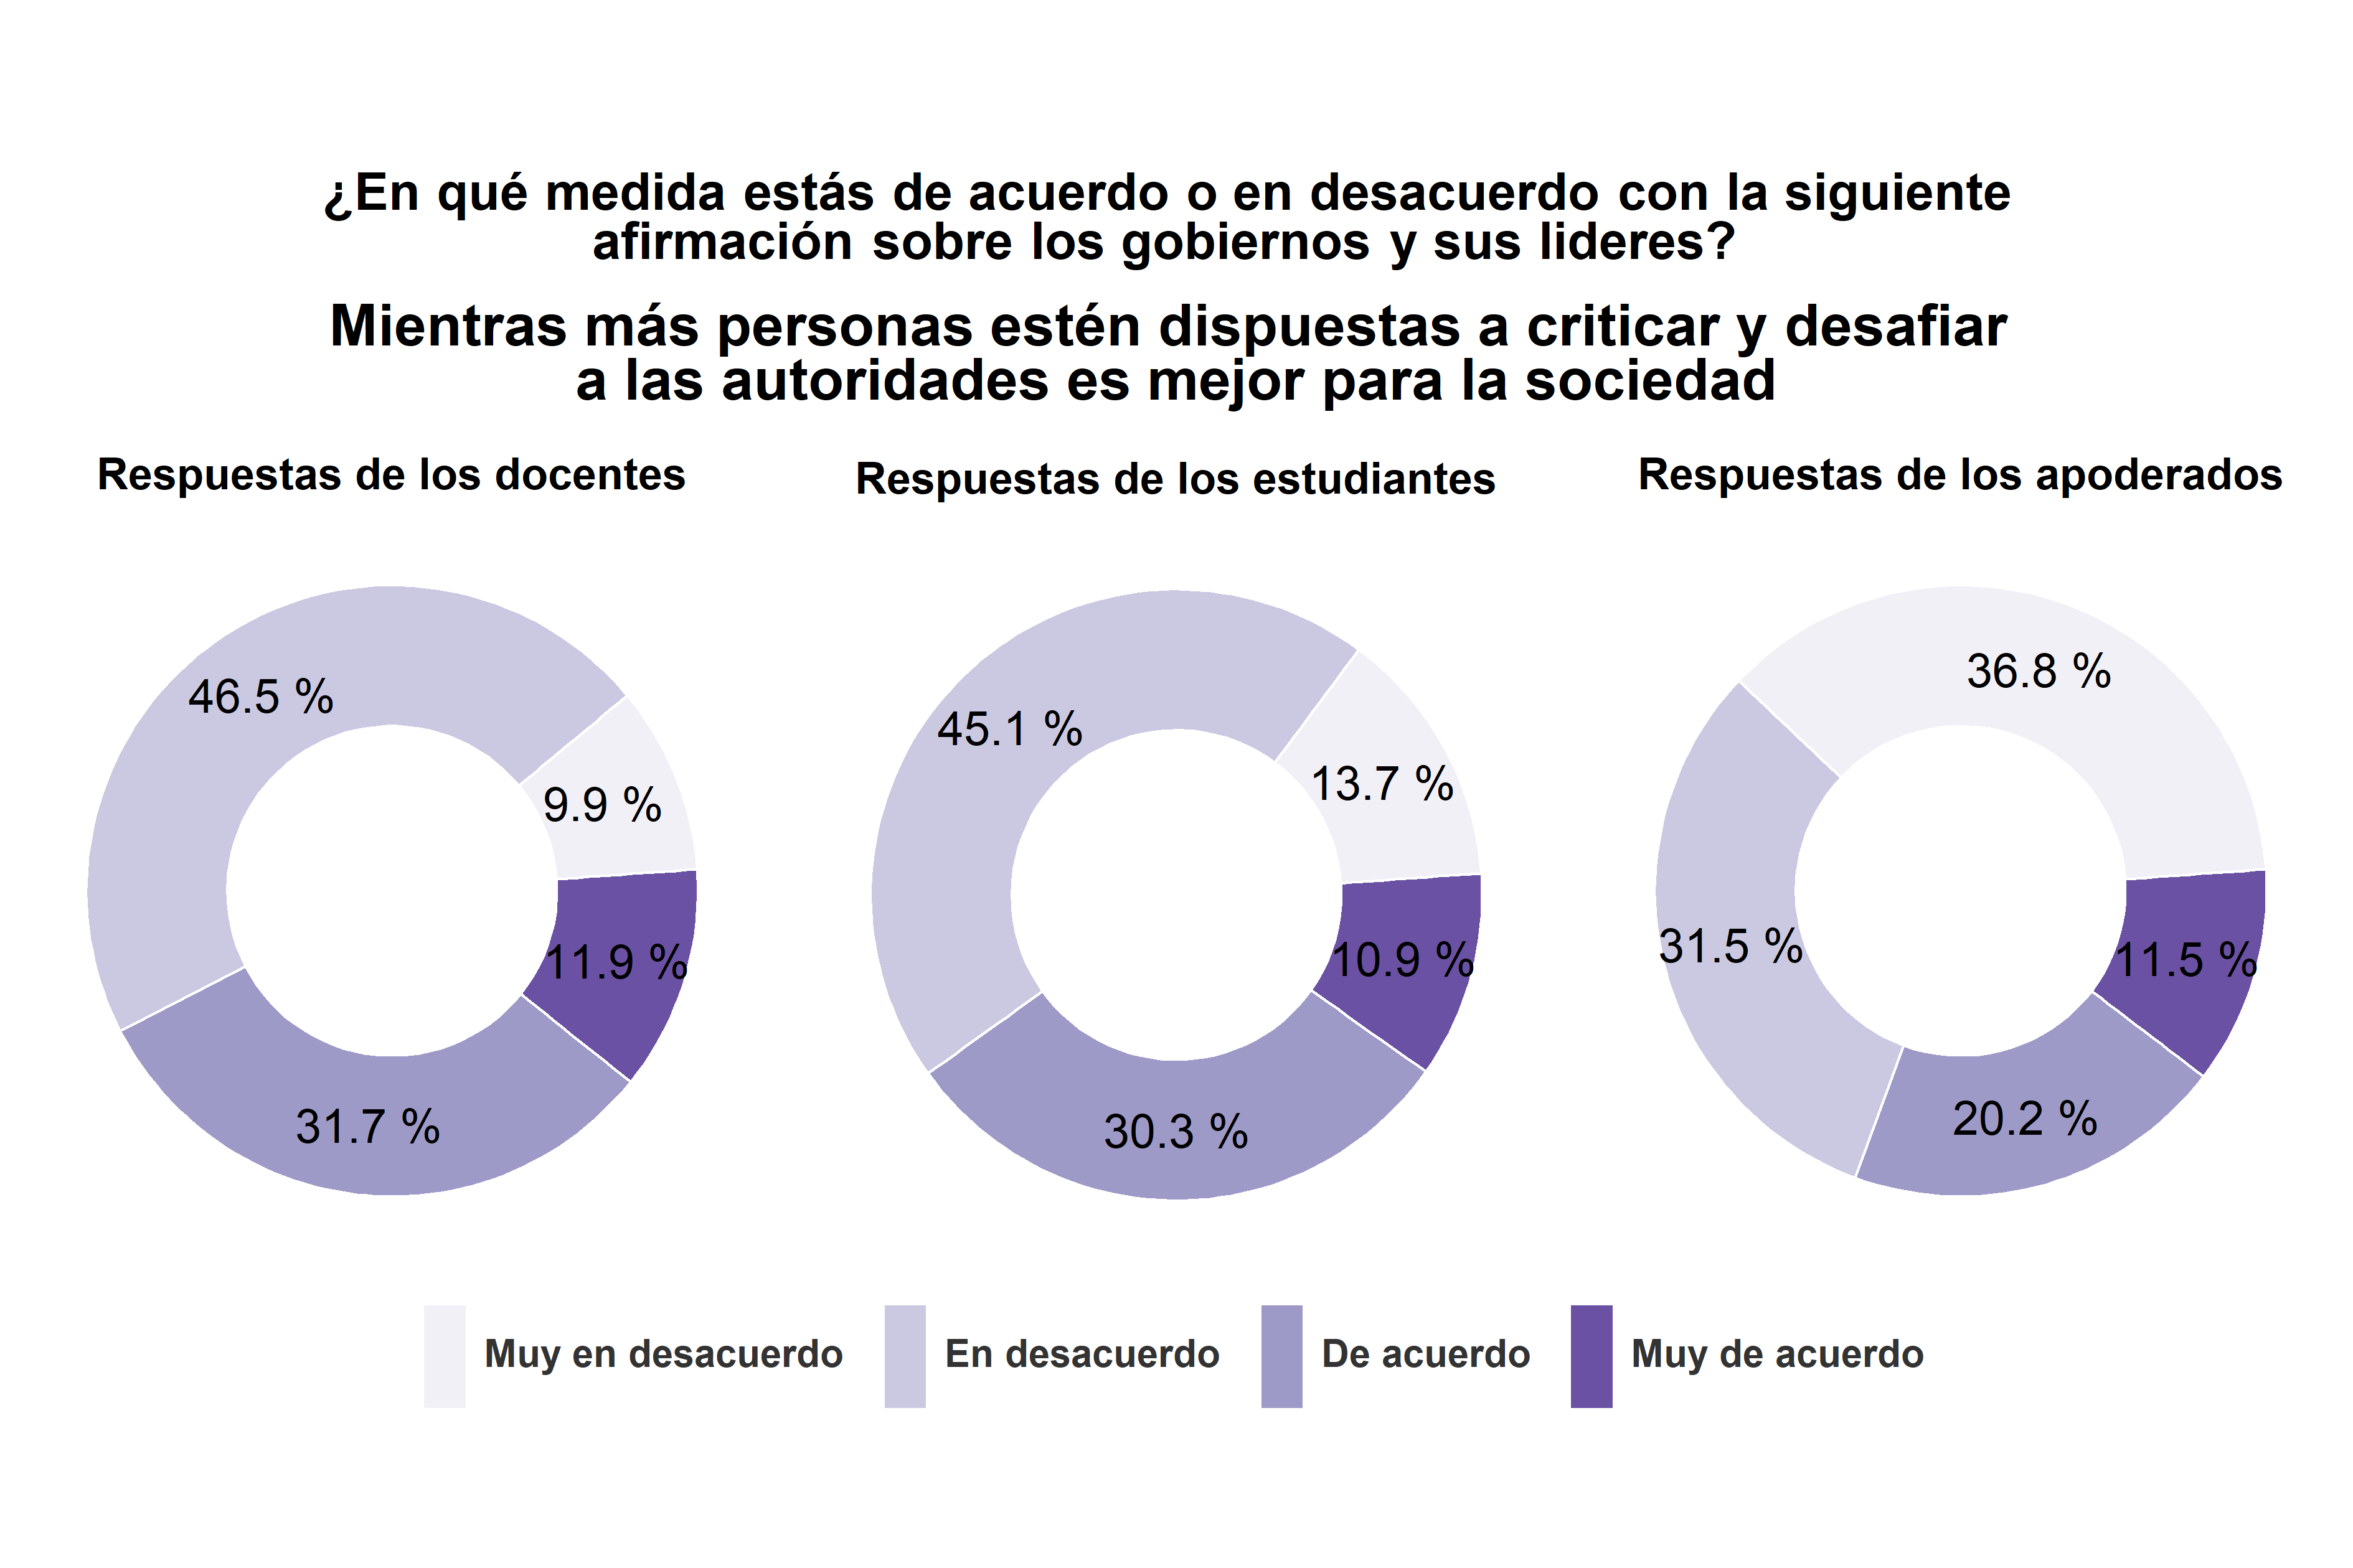
\includegraphics[width=52.49in]{images/graph_aut2} \end{center}

\begin{center}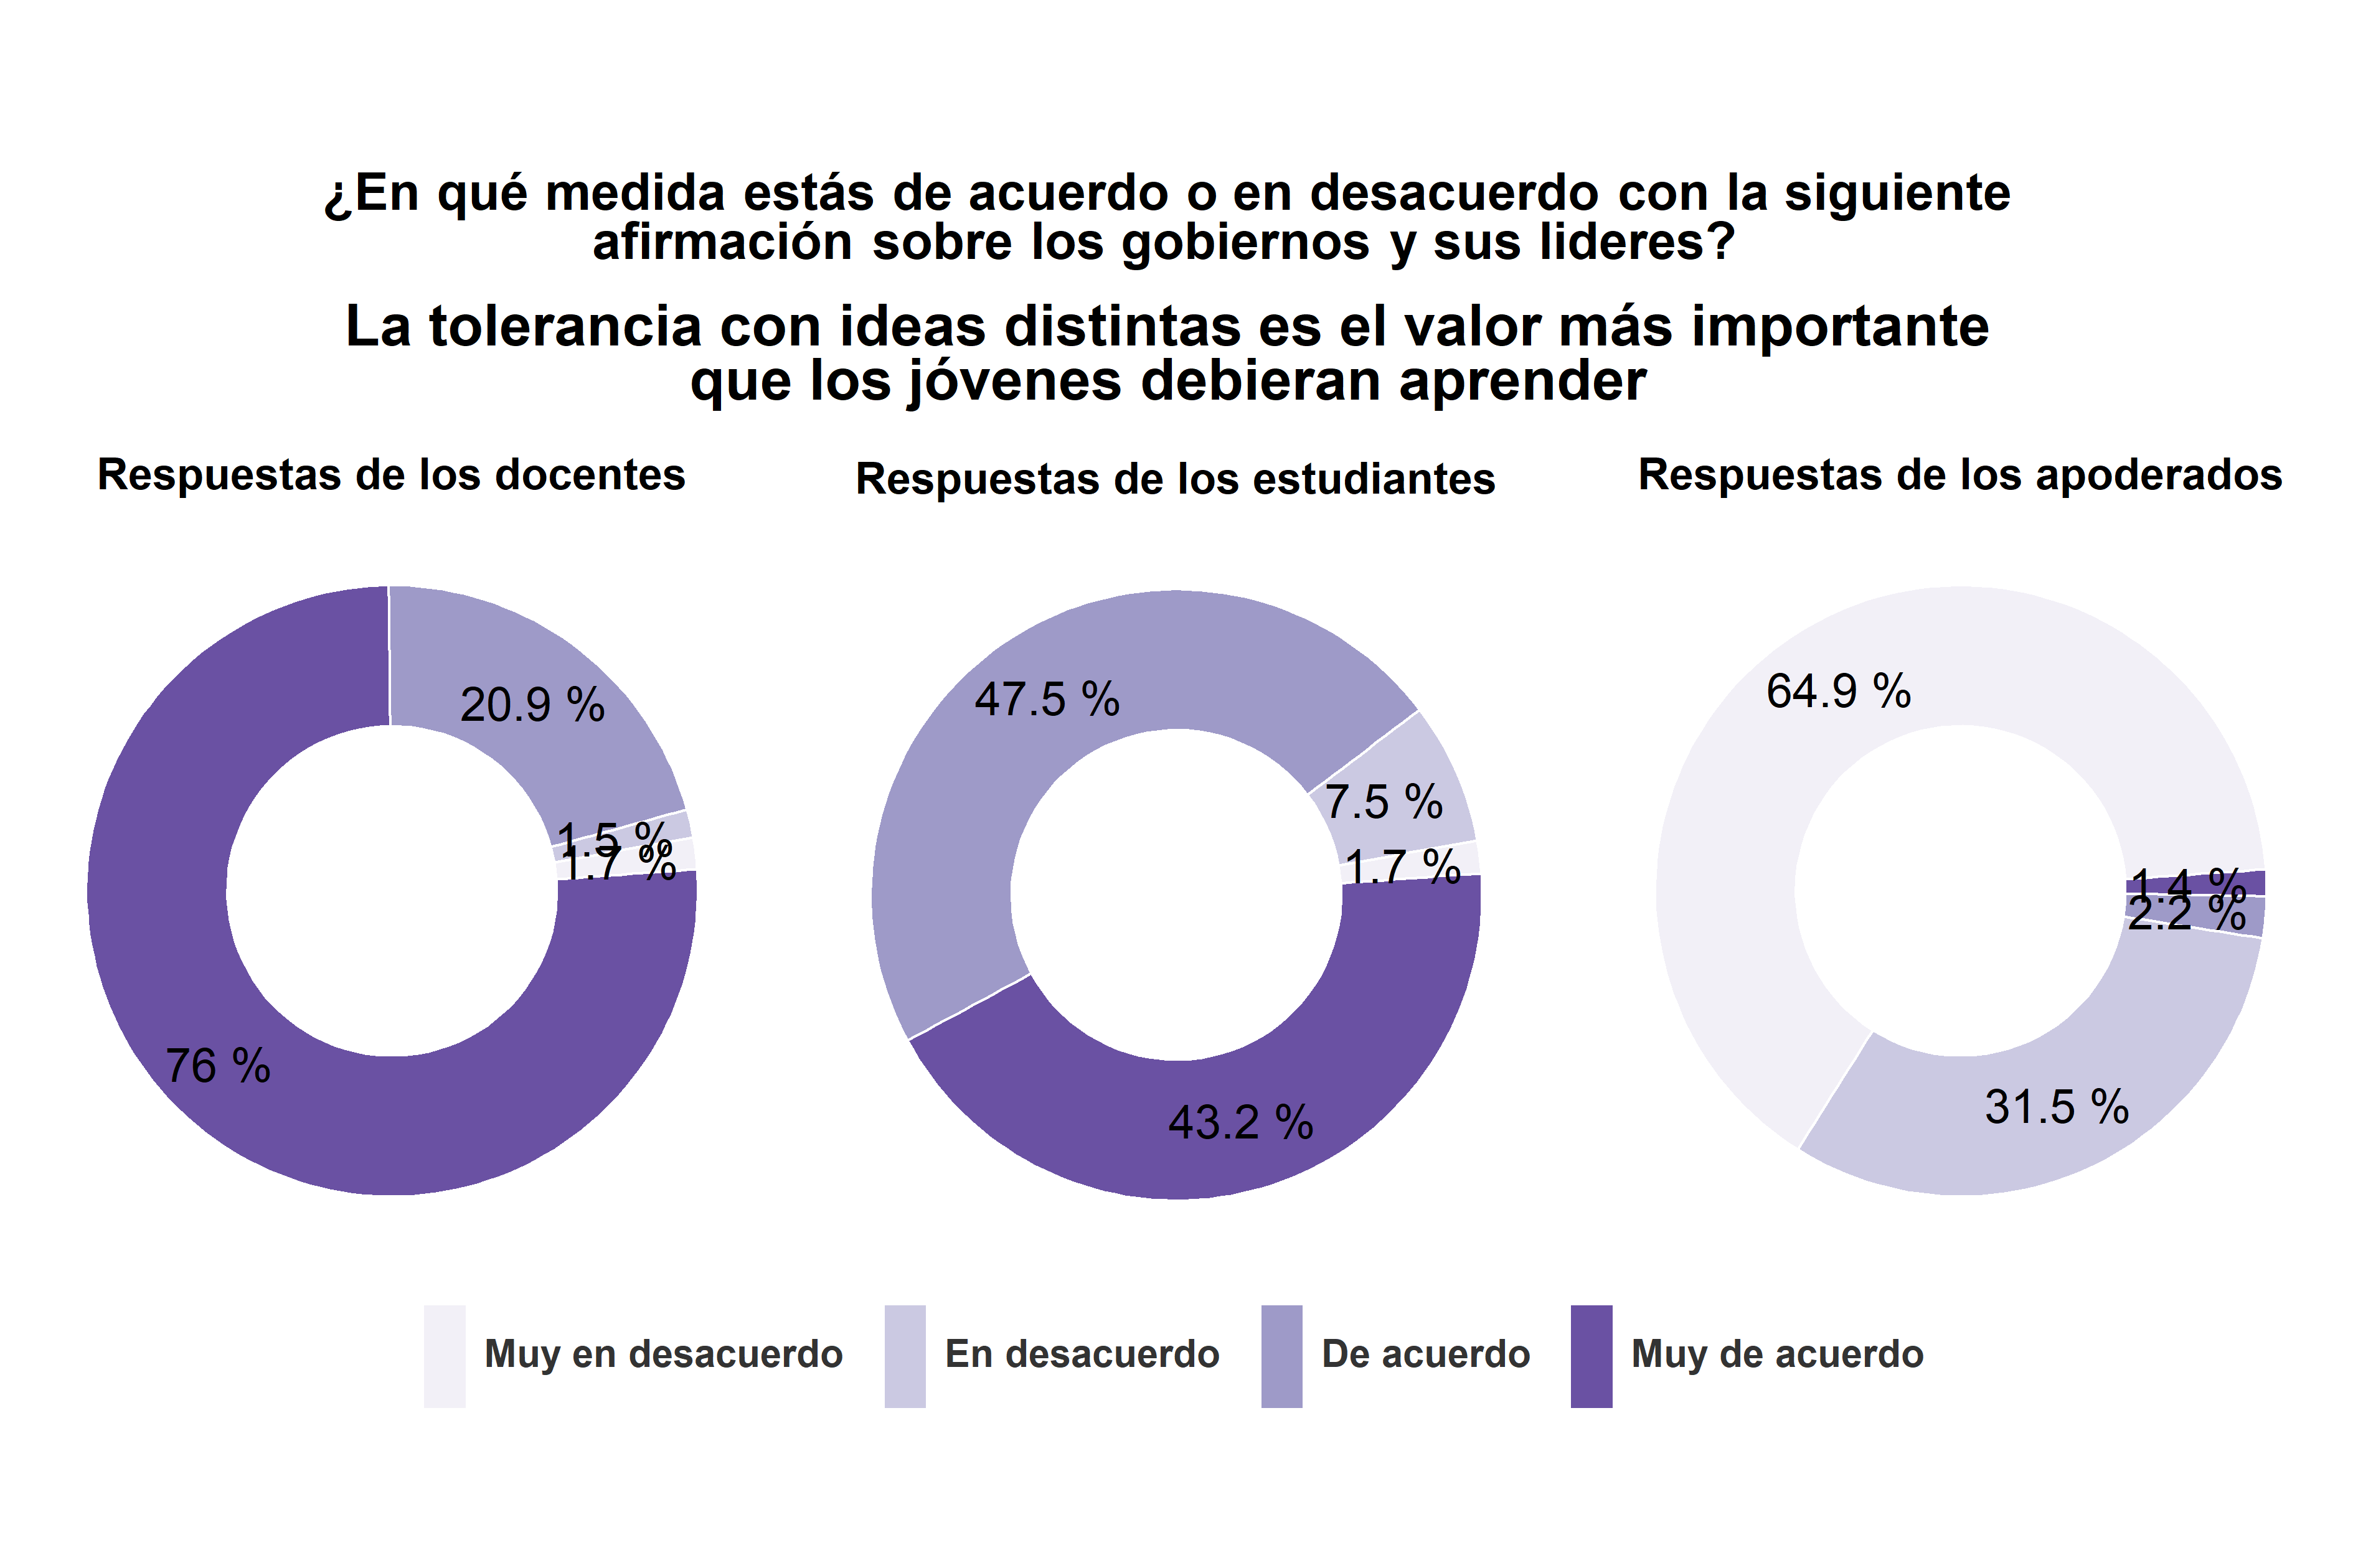
\includegraphics[width=52.49in]{images/graph_aut3} \end{center}

\begin{center}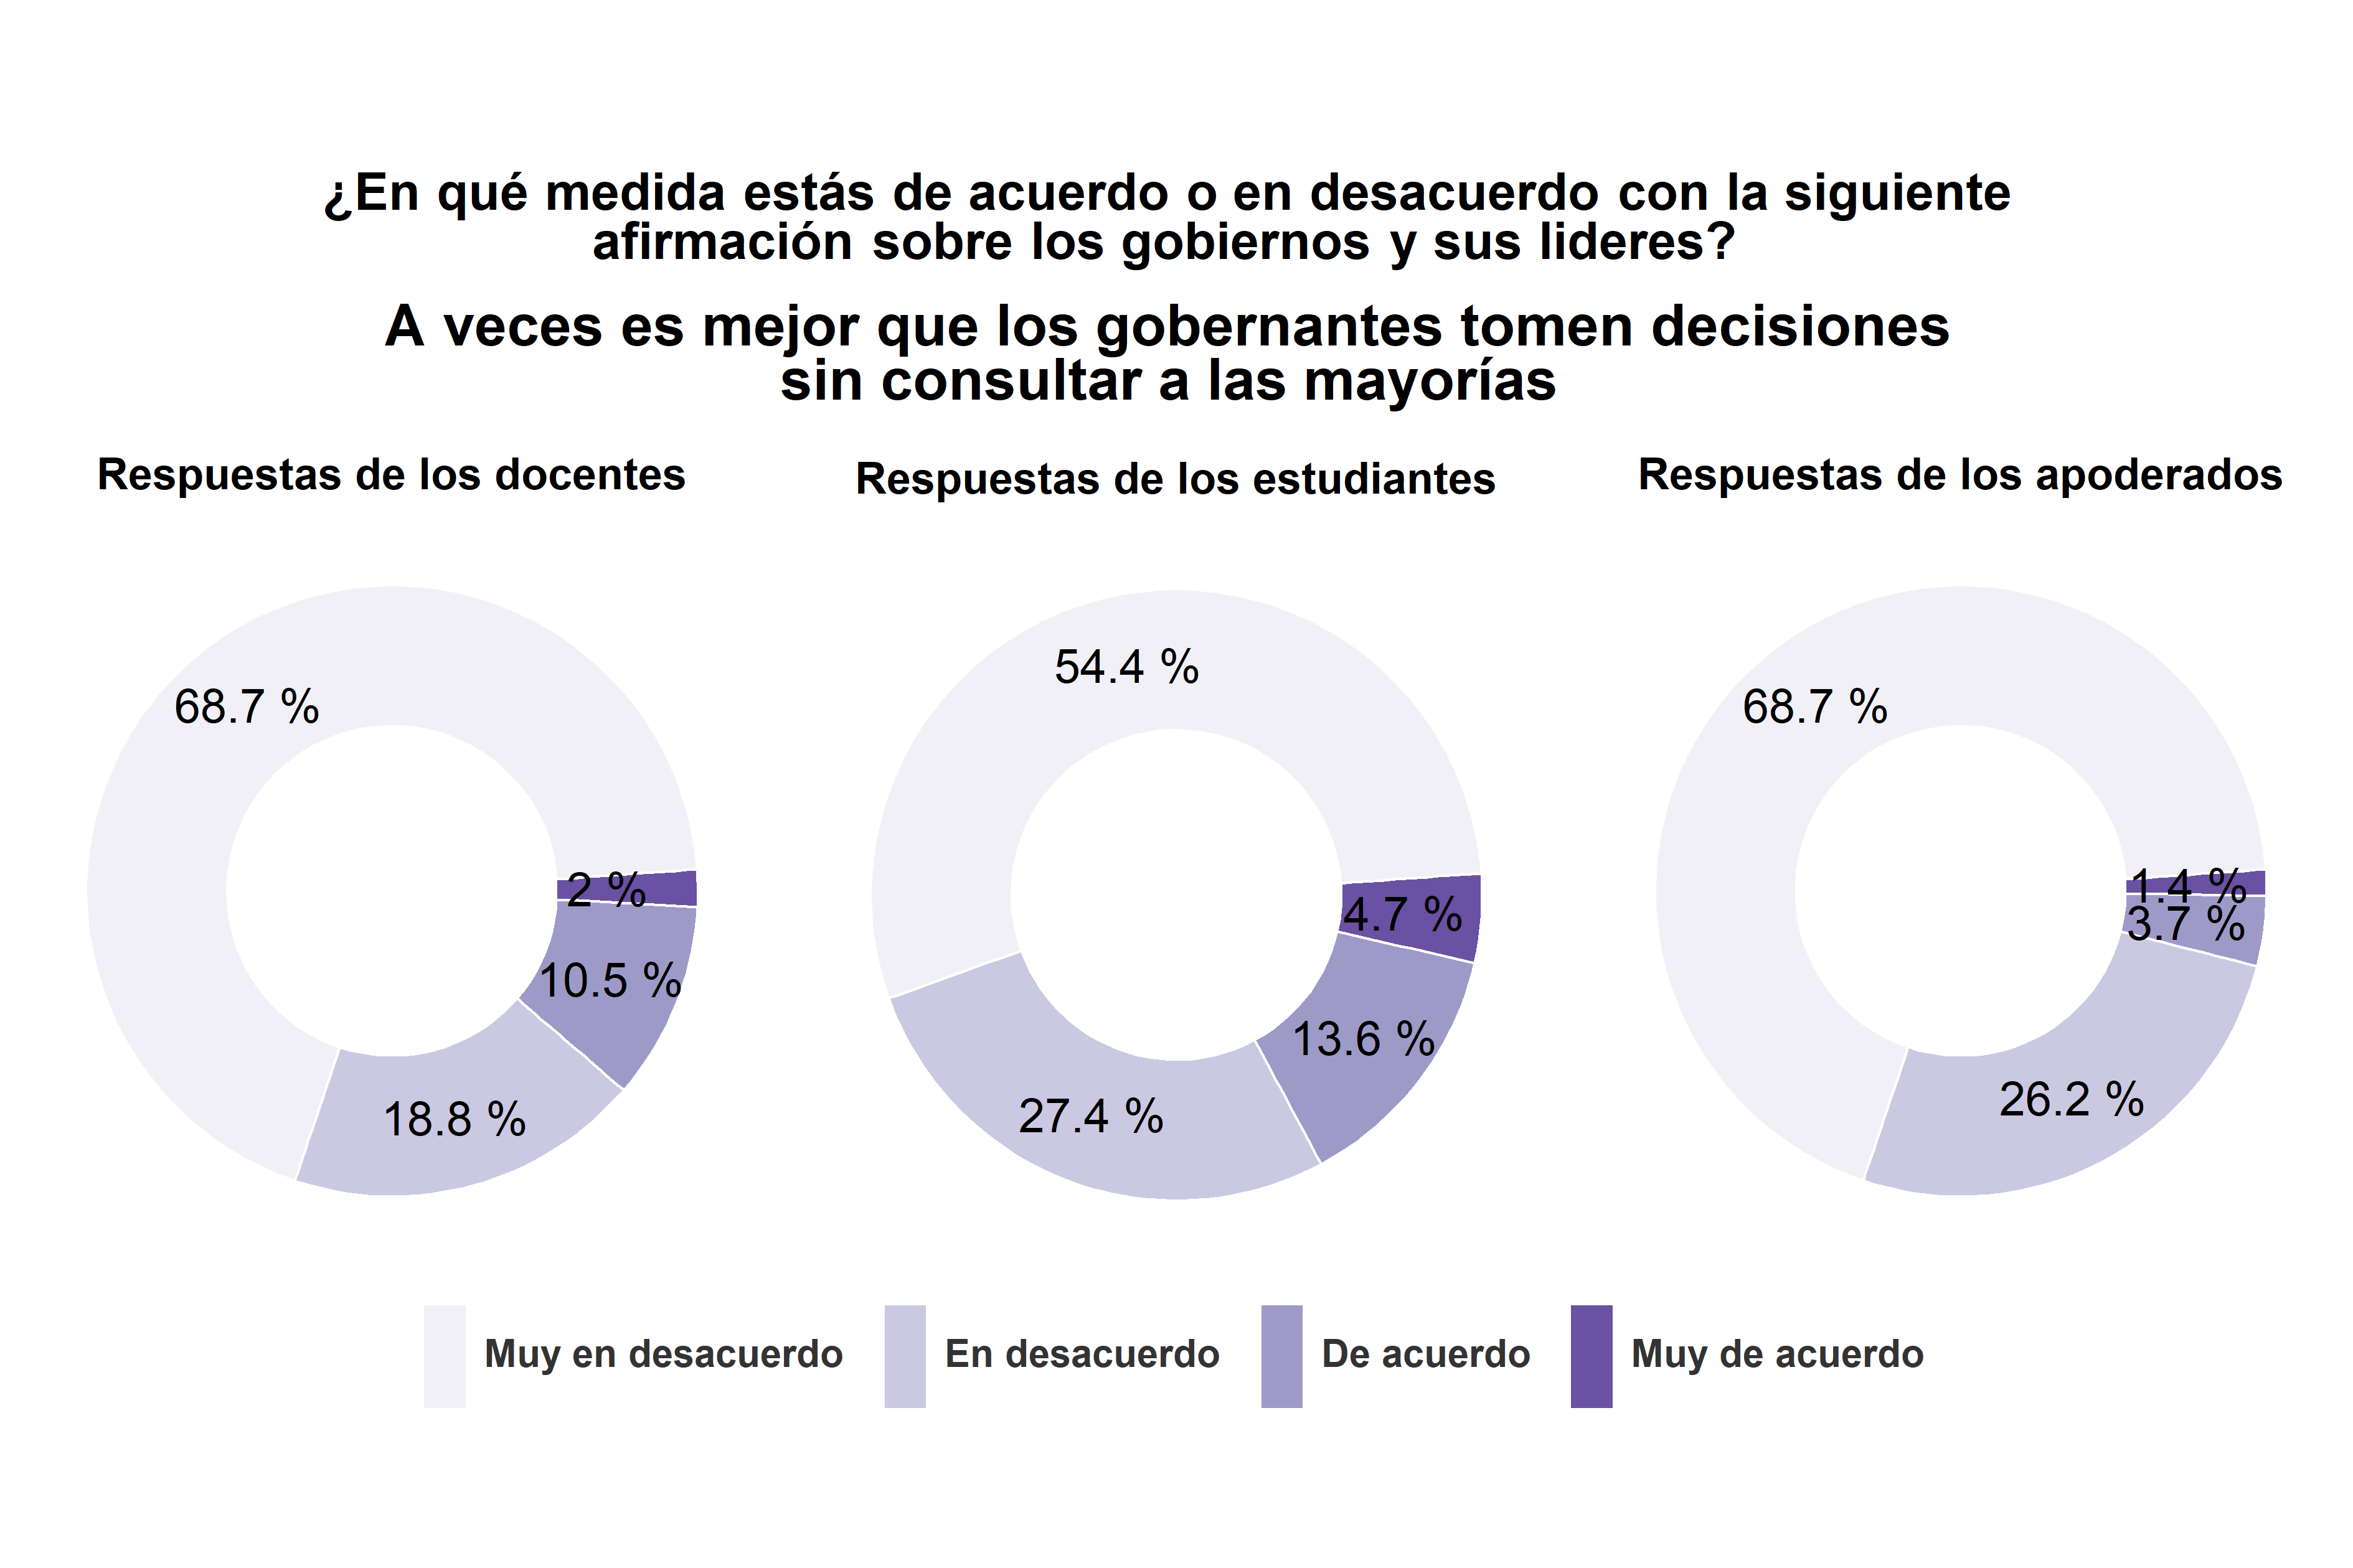
\includegraphics[width=52.49in]{images/graph_aut4} \end{center}

\begin{center}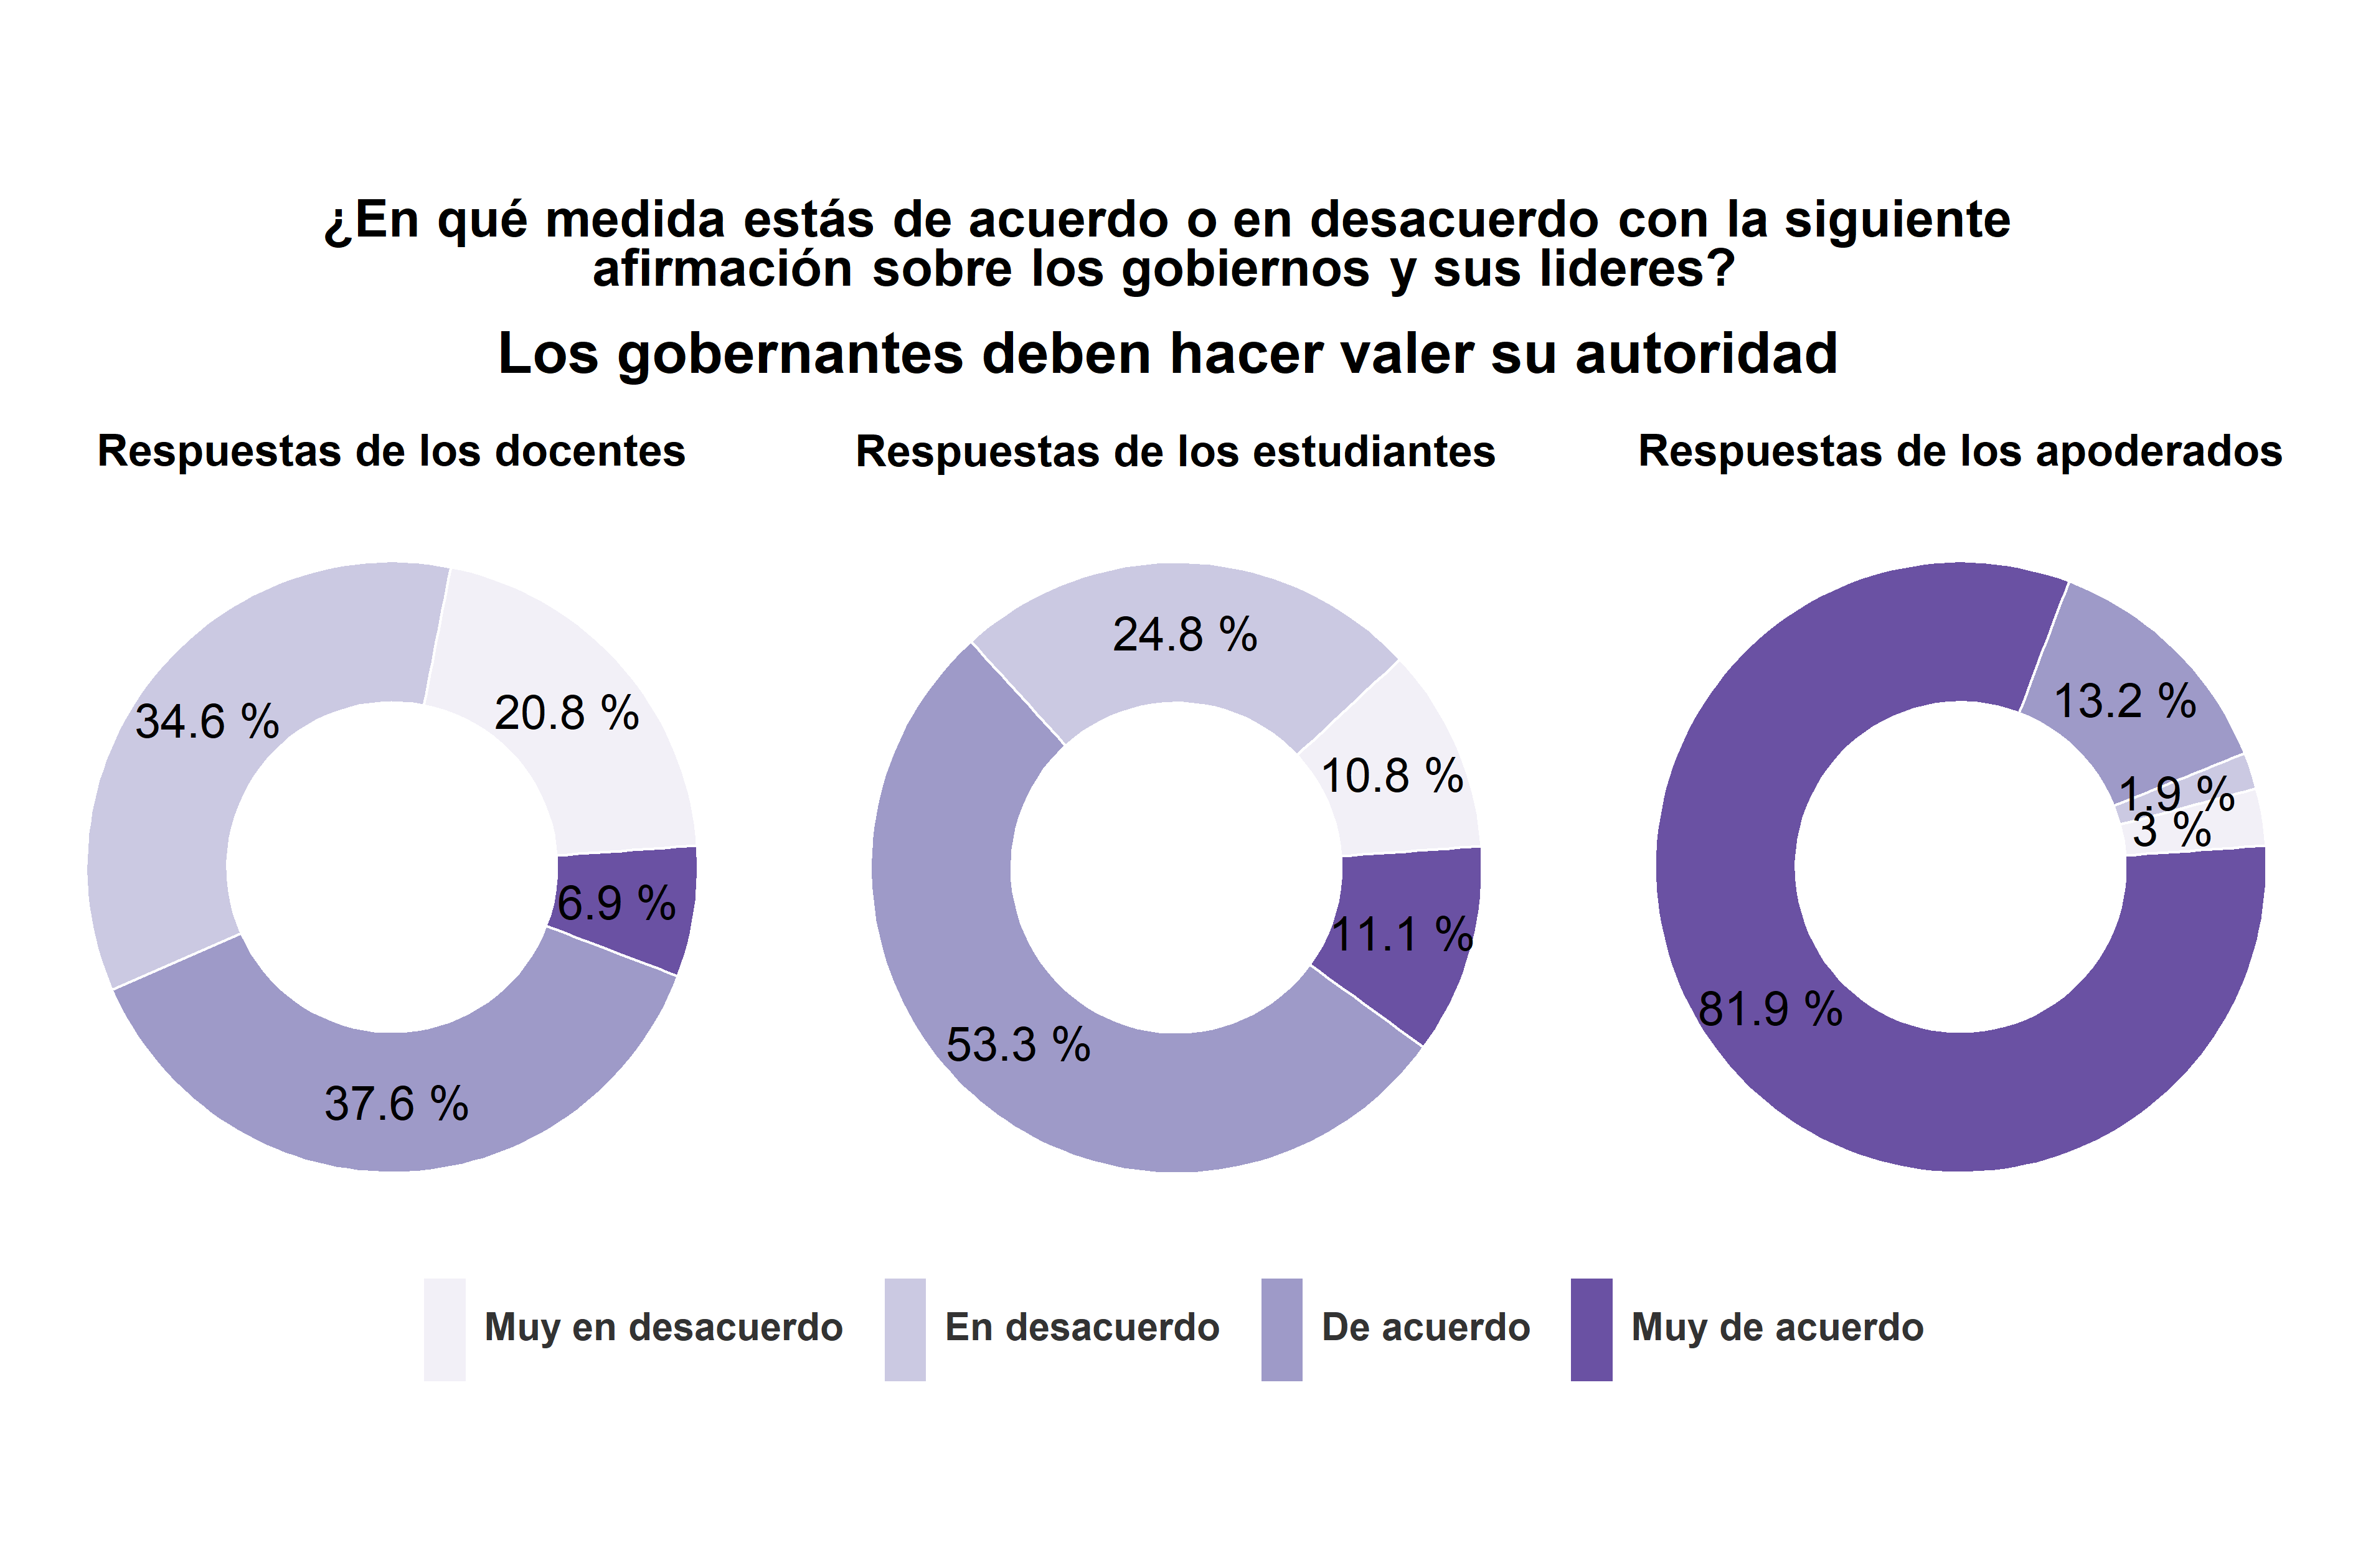
\includegraphics[width=52.49in]{images/graph_aut5} \end{center}

\begin{center}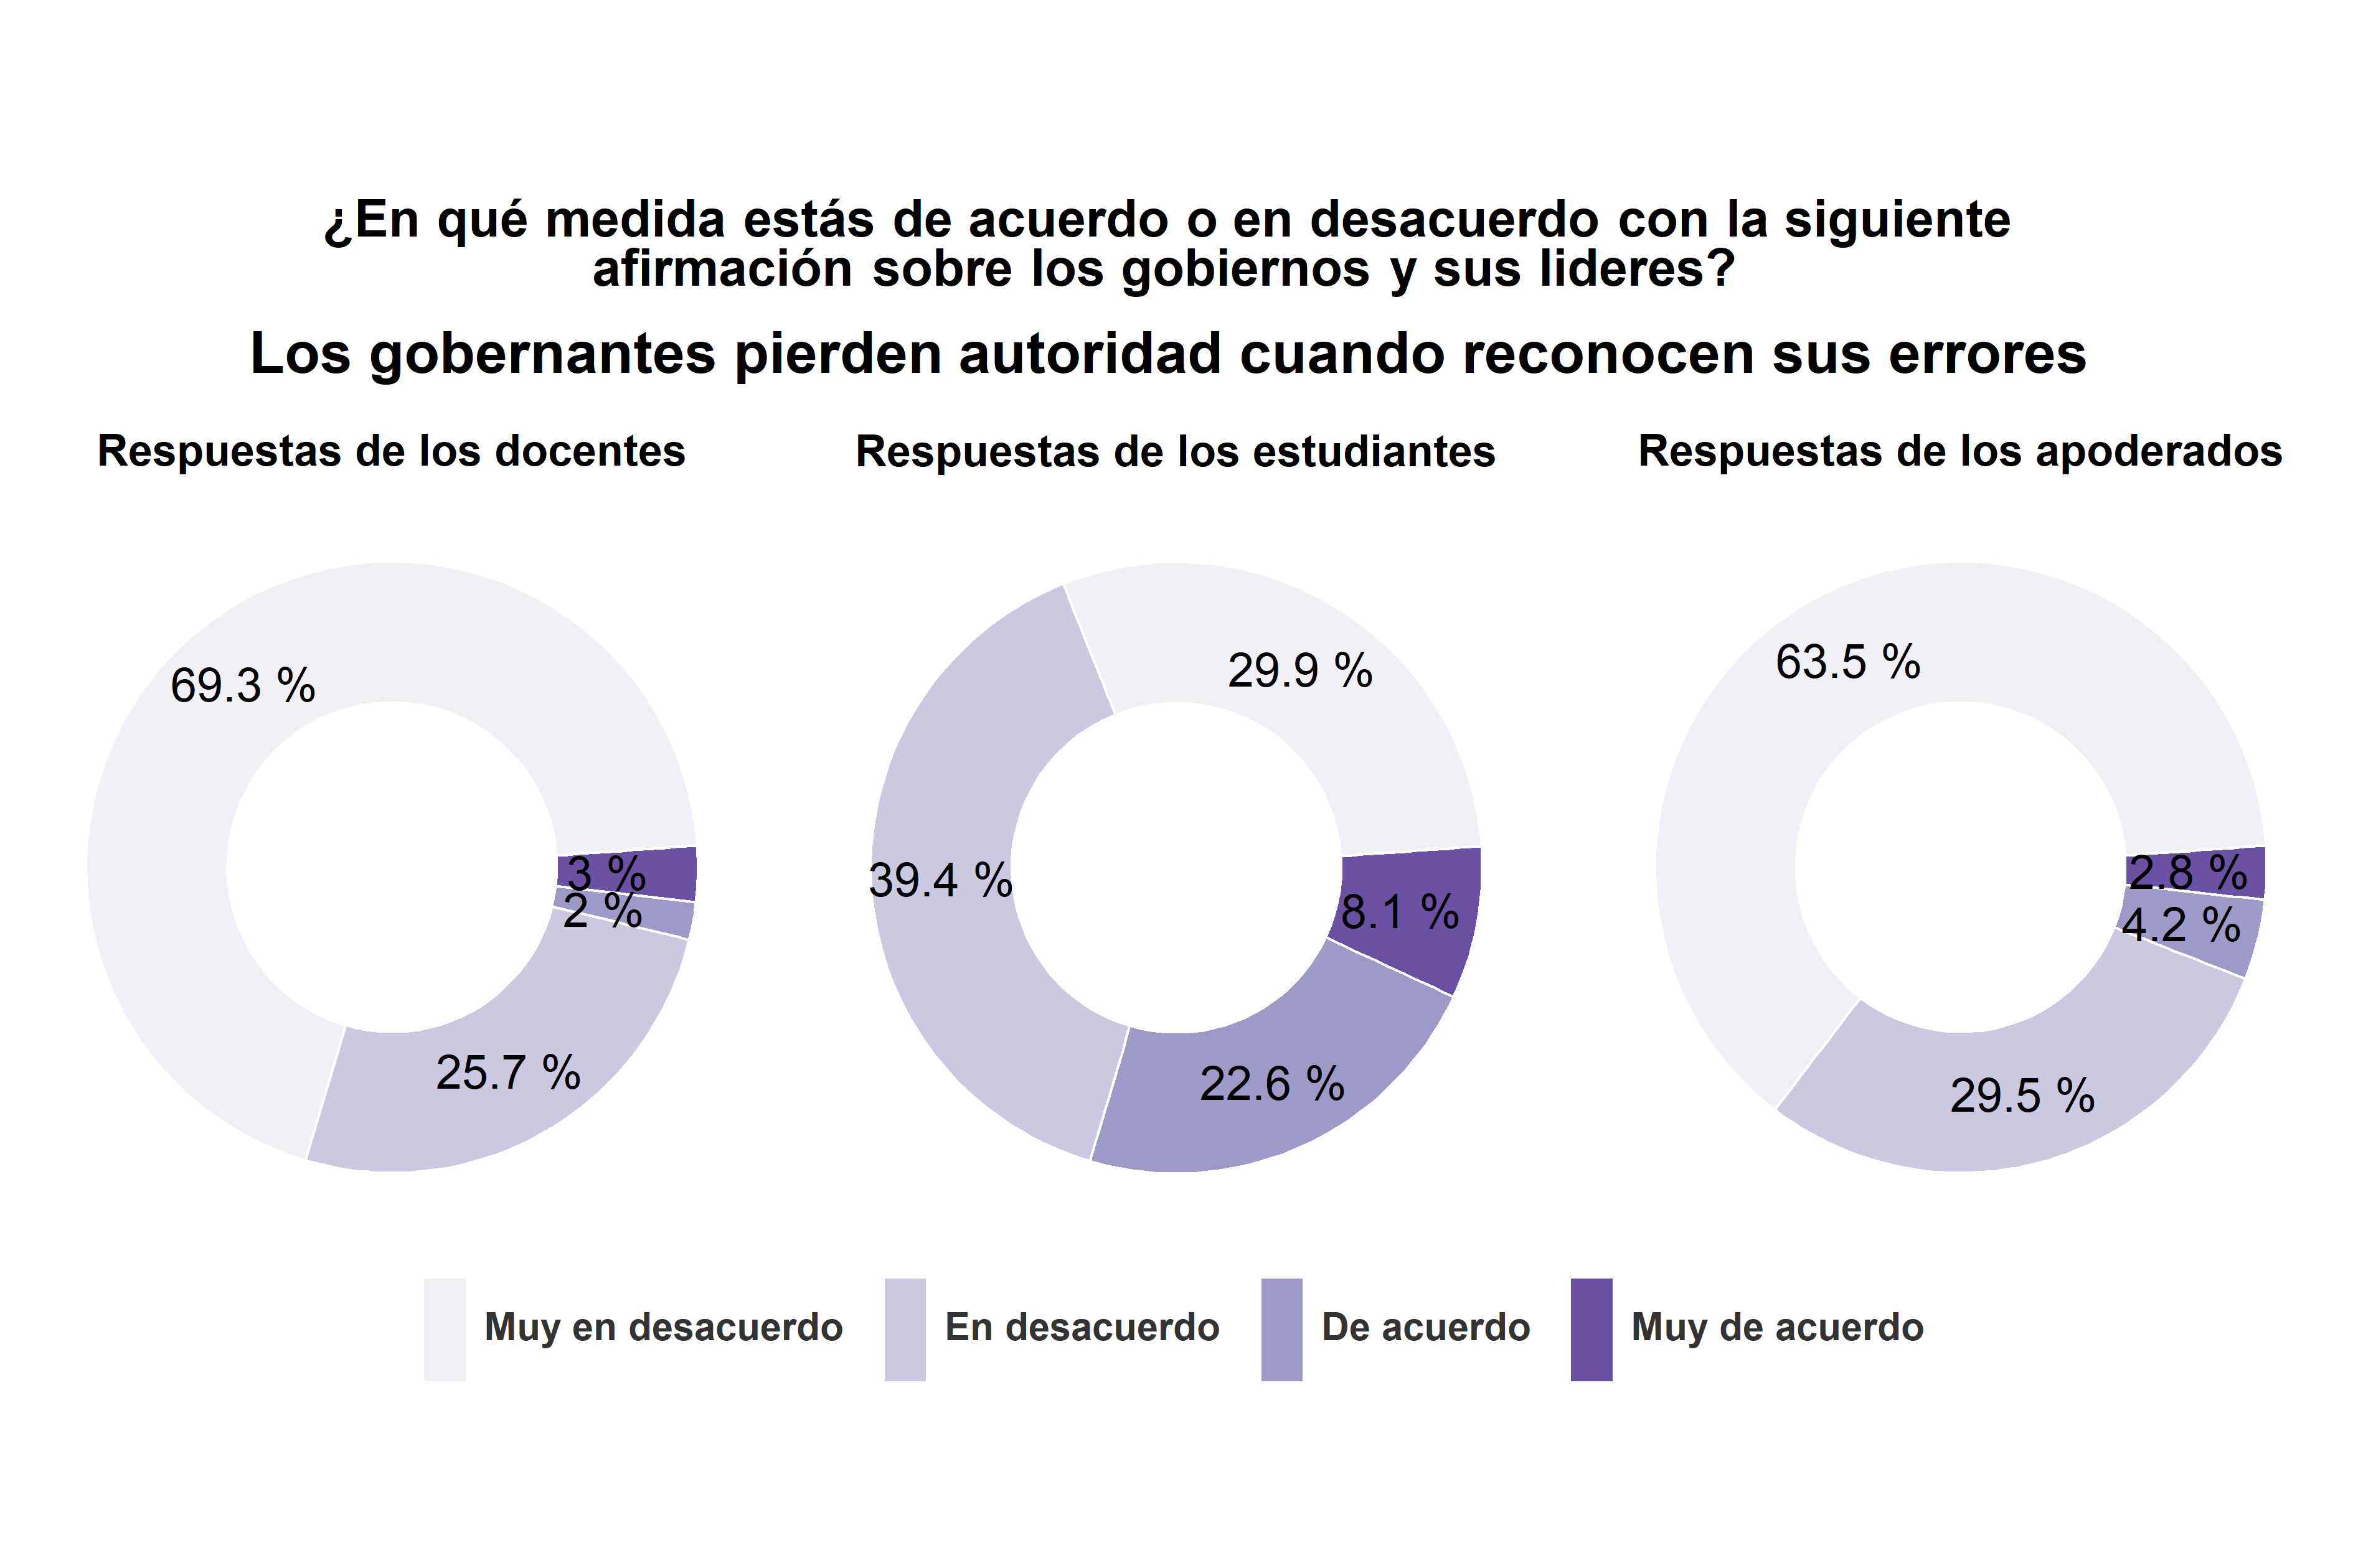
\includegraphics[width=52.49in]{images/graph_aut6} \end{center}

\begin{center}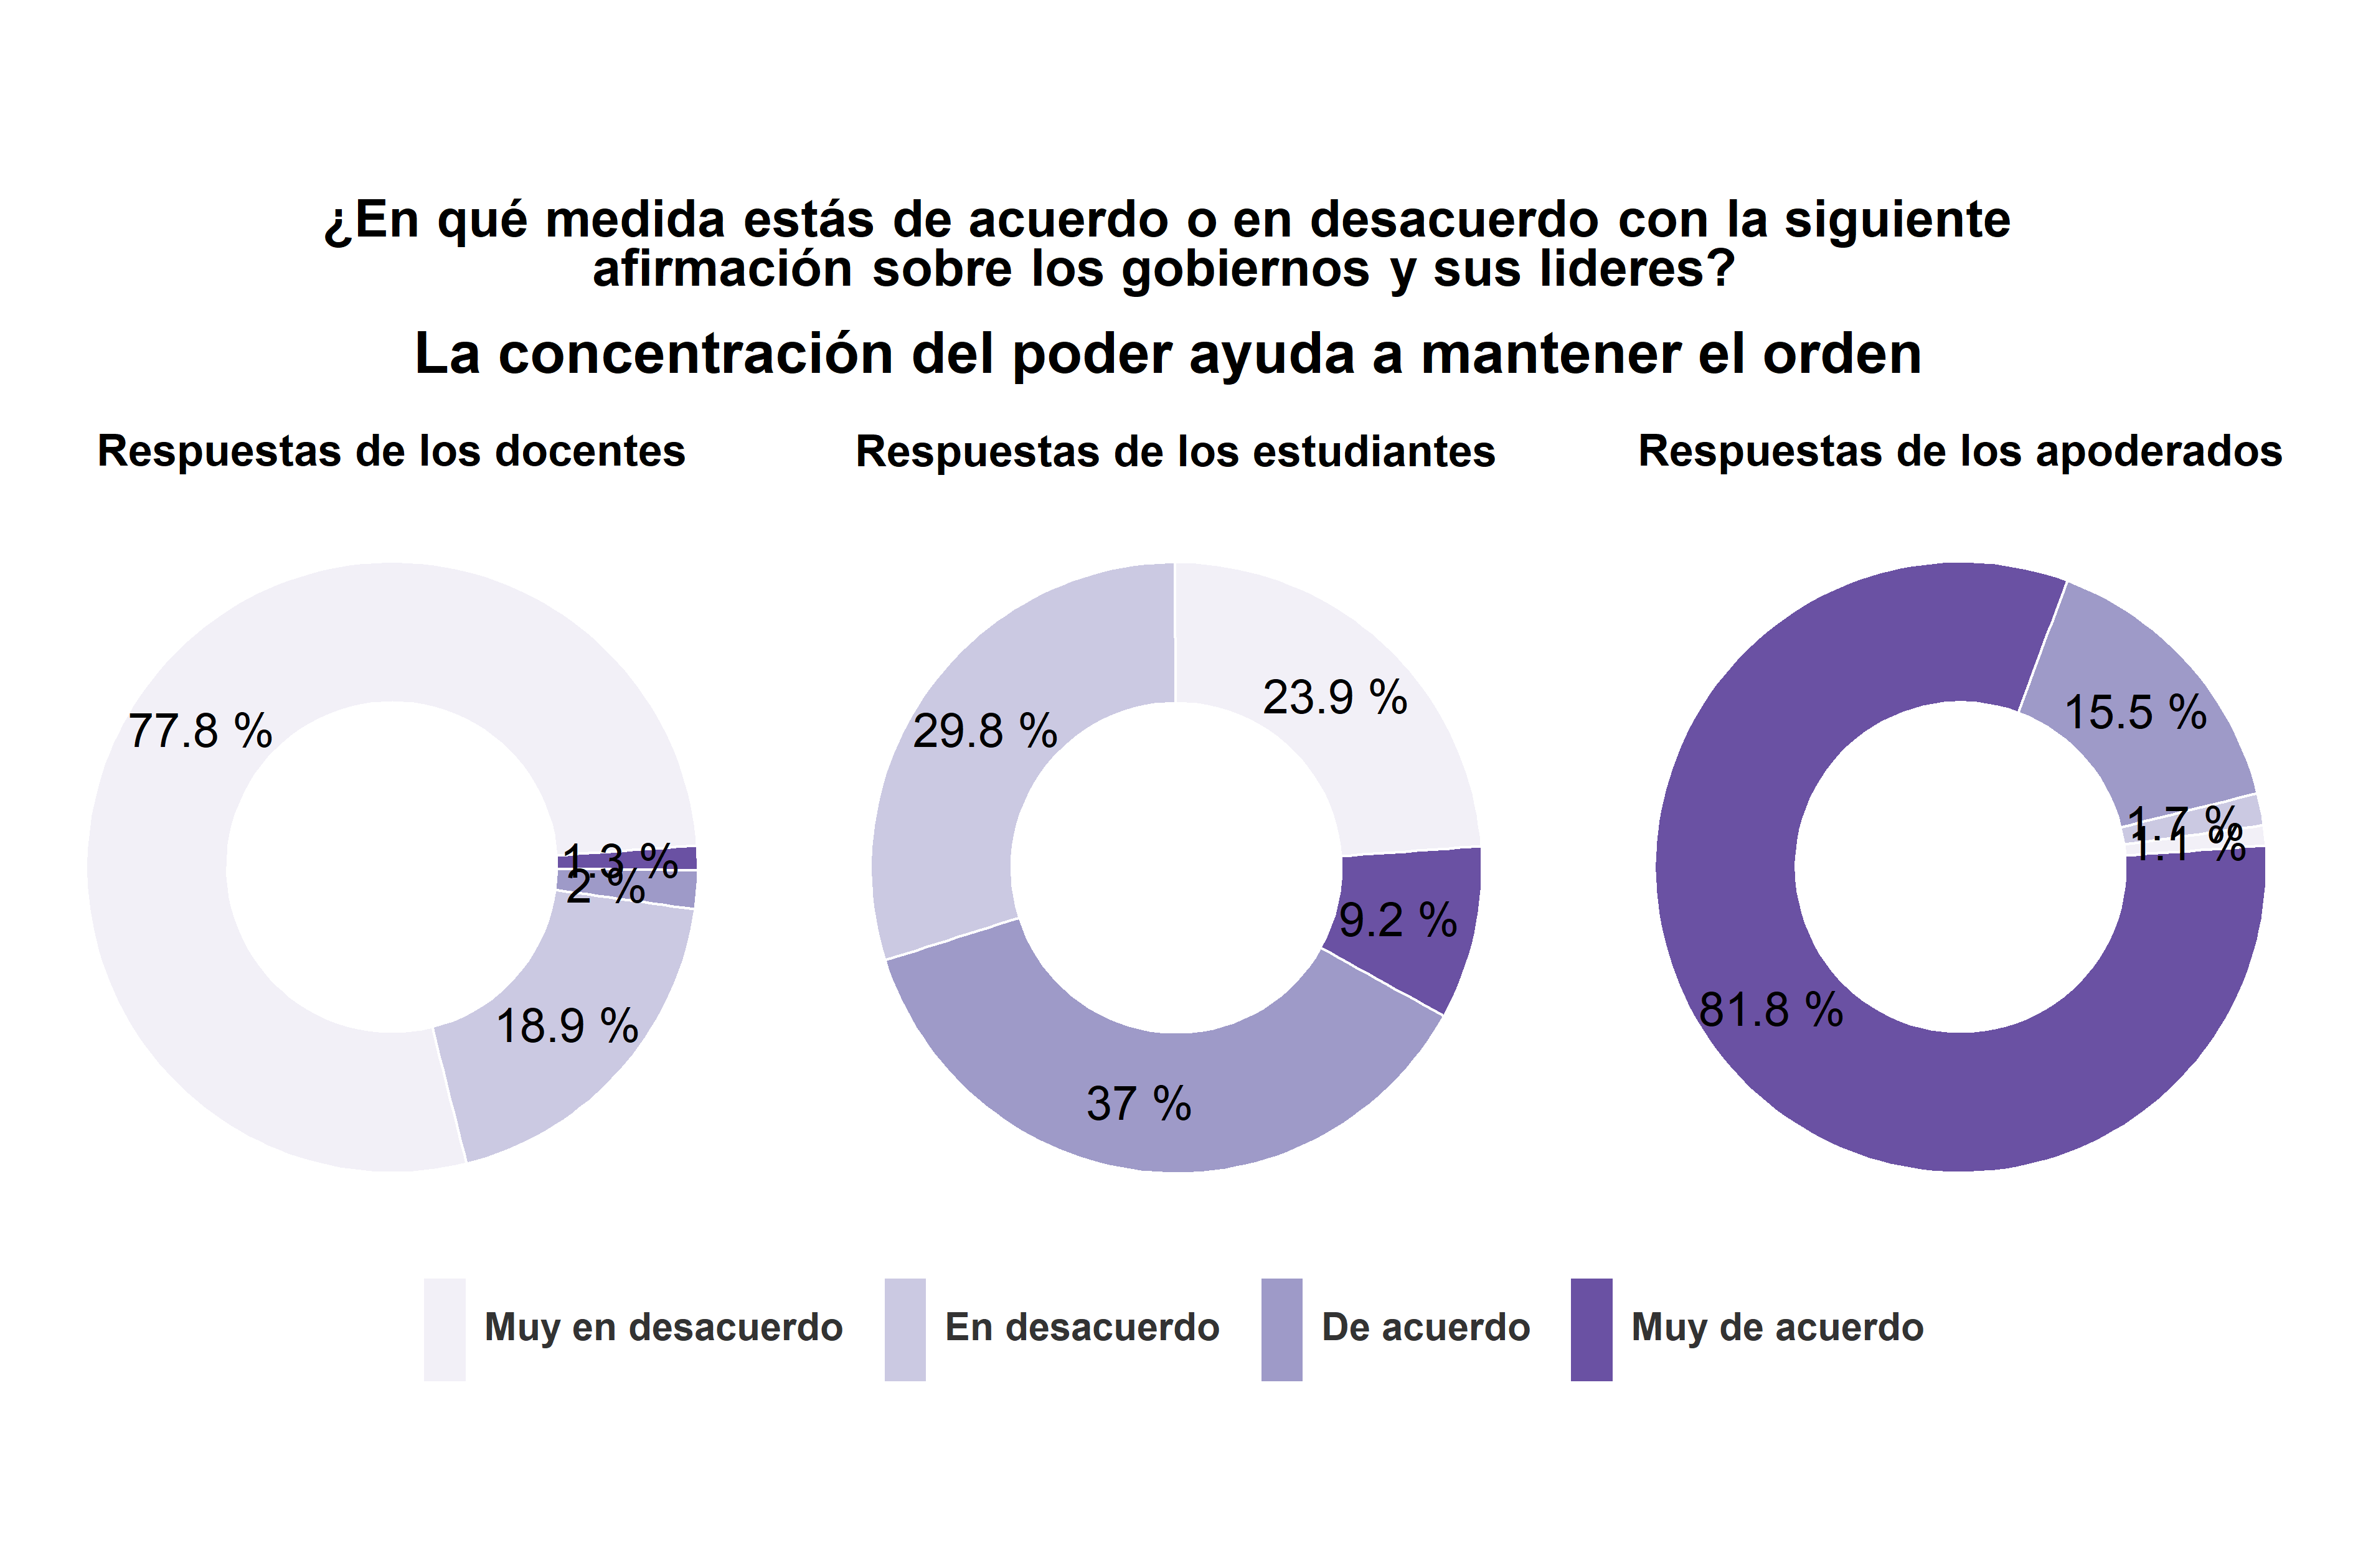
\includegraphics[width=52.49in]{images/graph_aut7} \end{center}

\begin{center}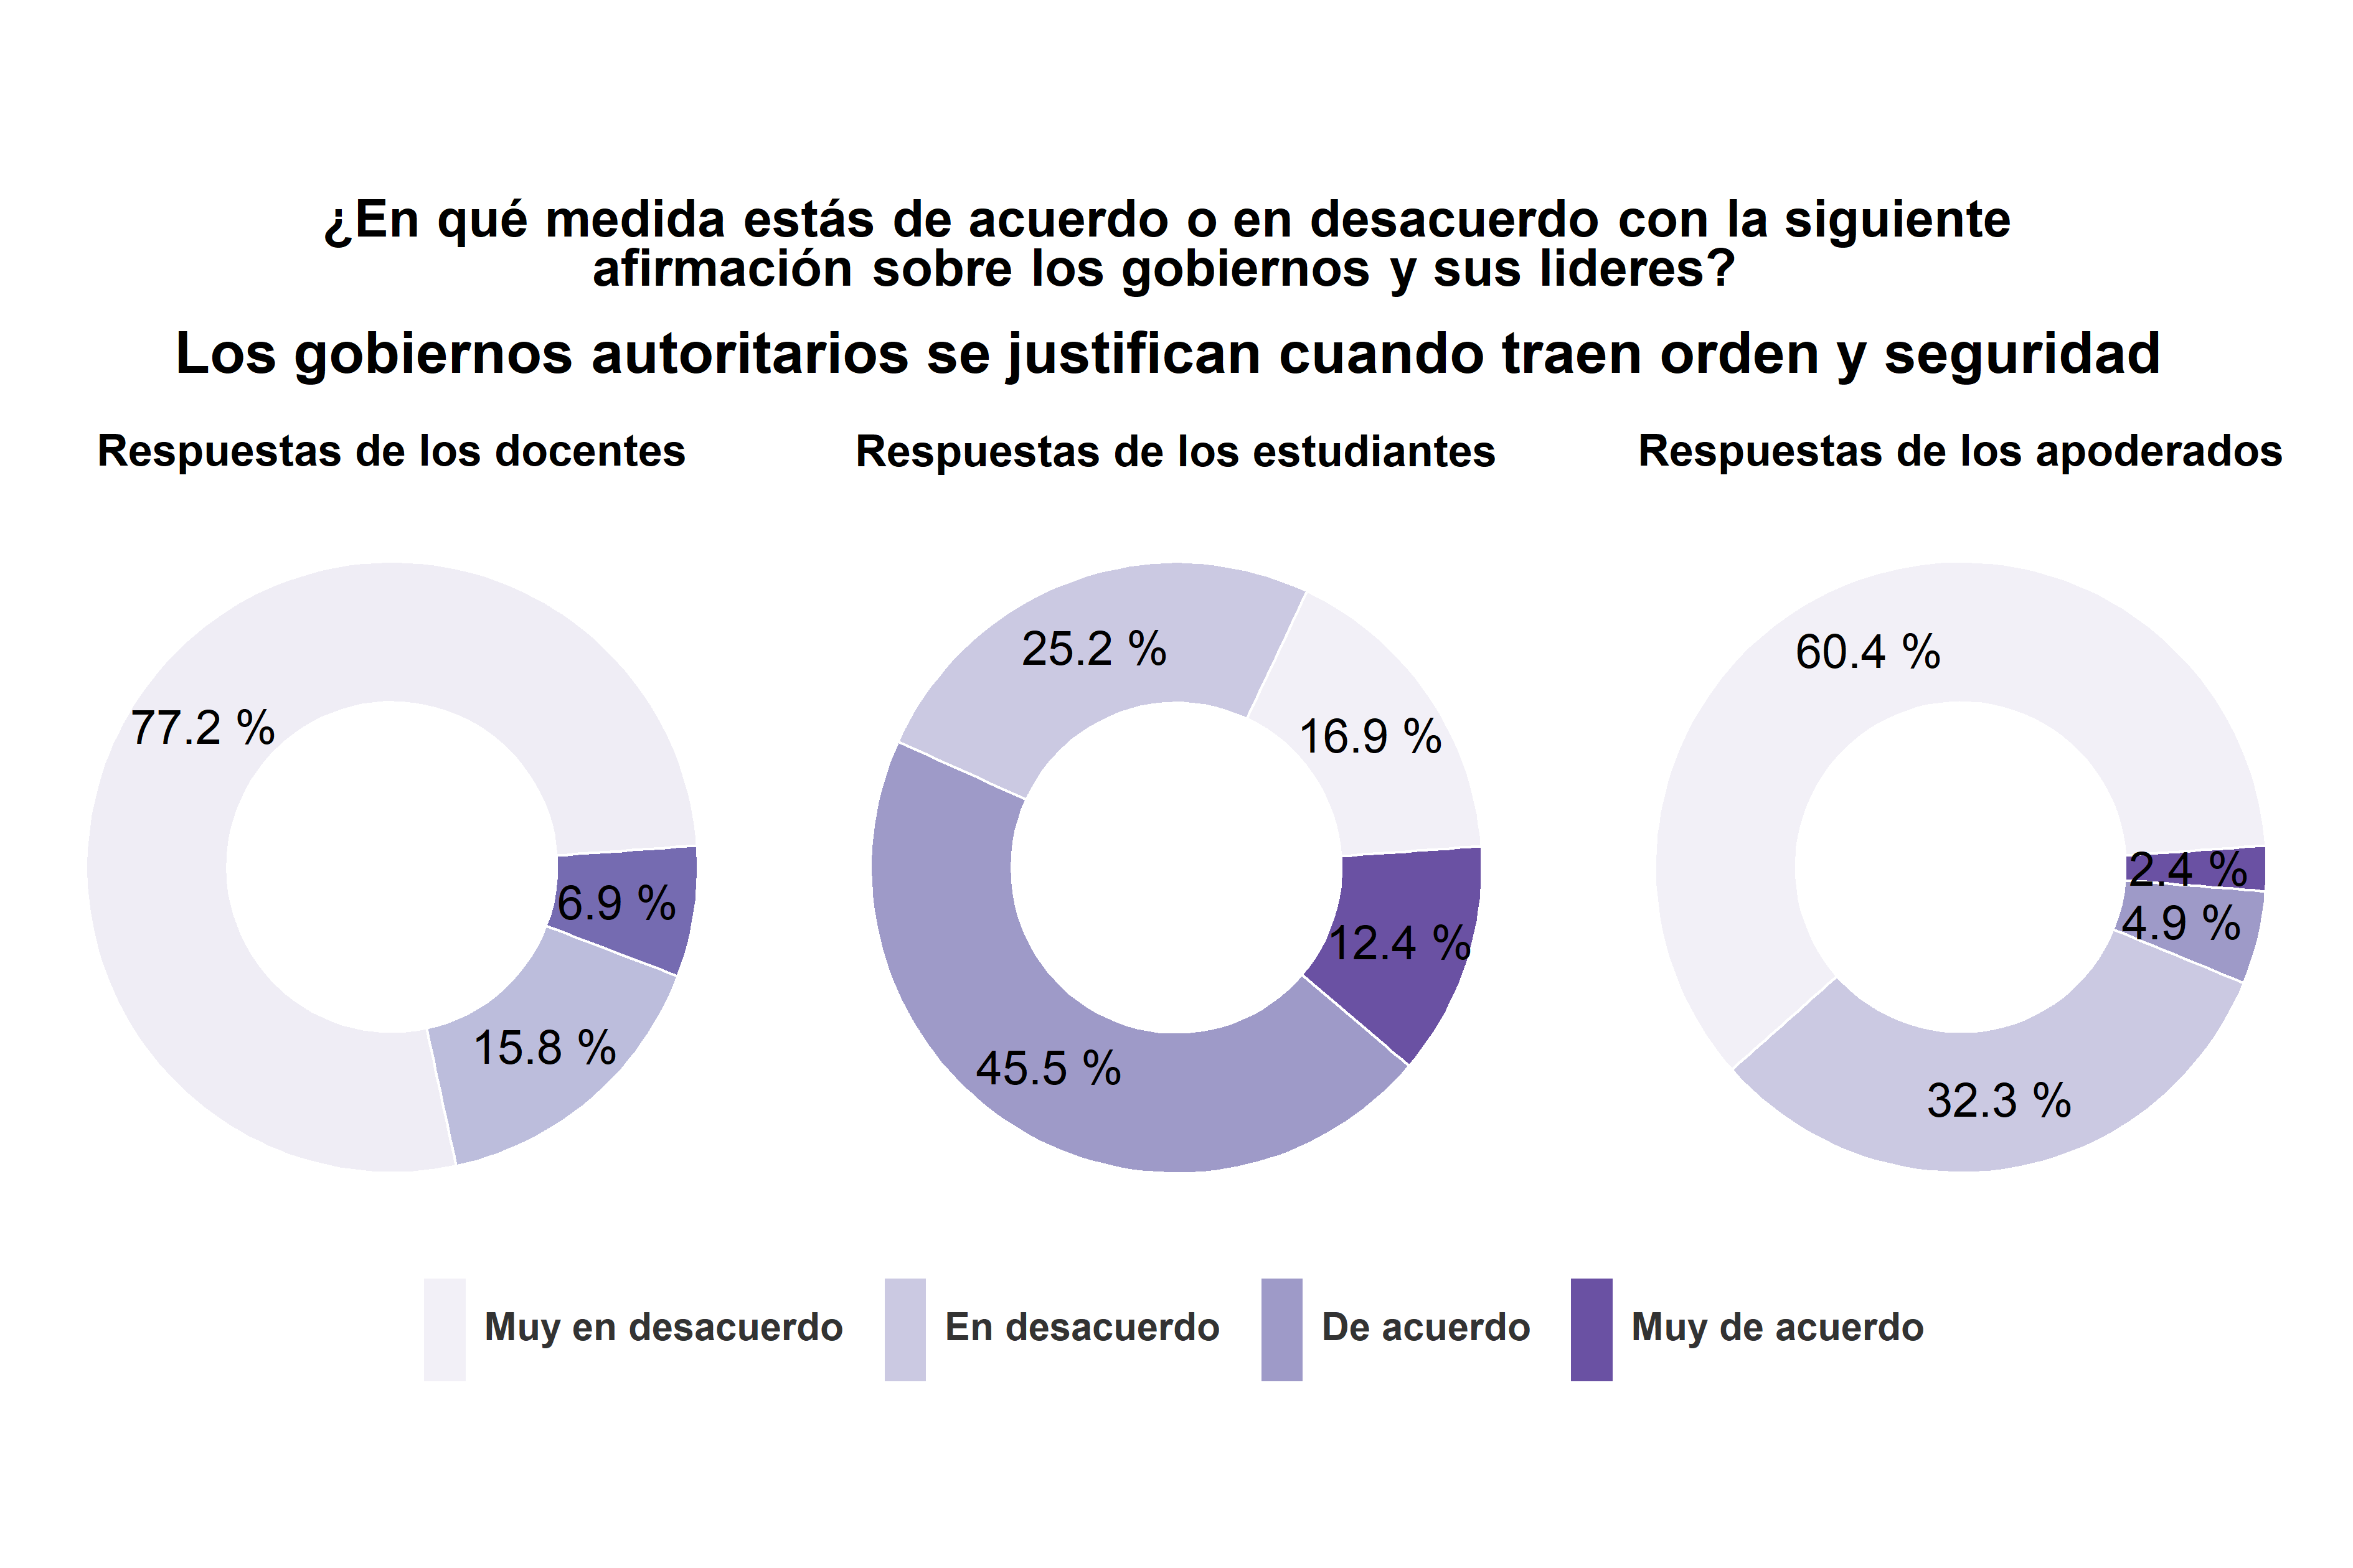
\includegraphics[width=52.49in]{images/graph_aut8} \end{center}

\begin{center}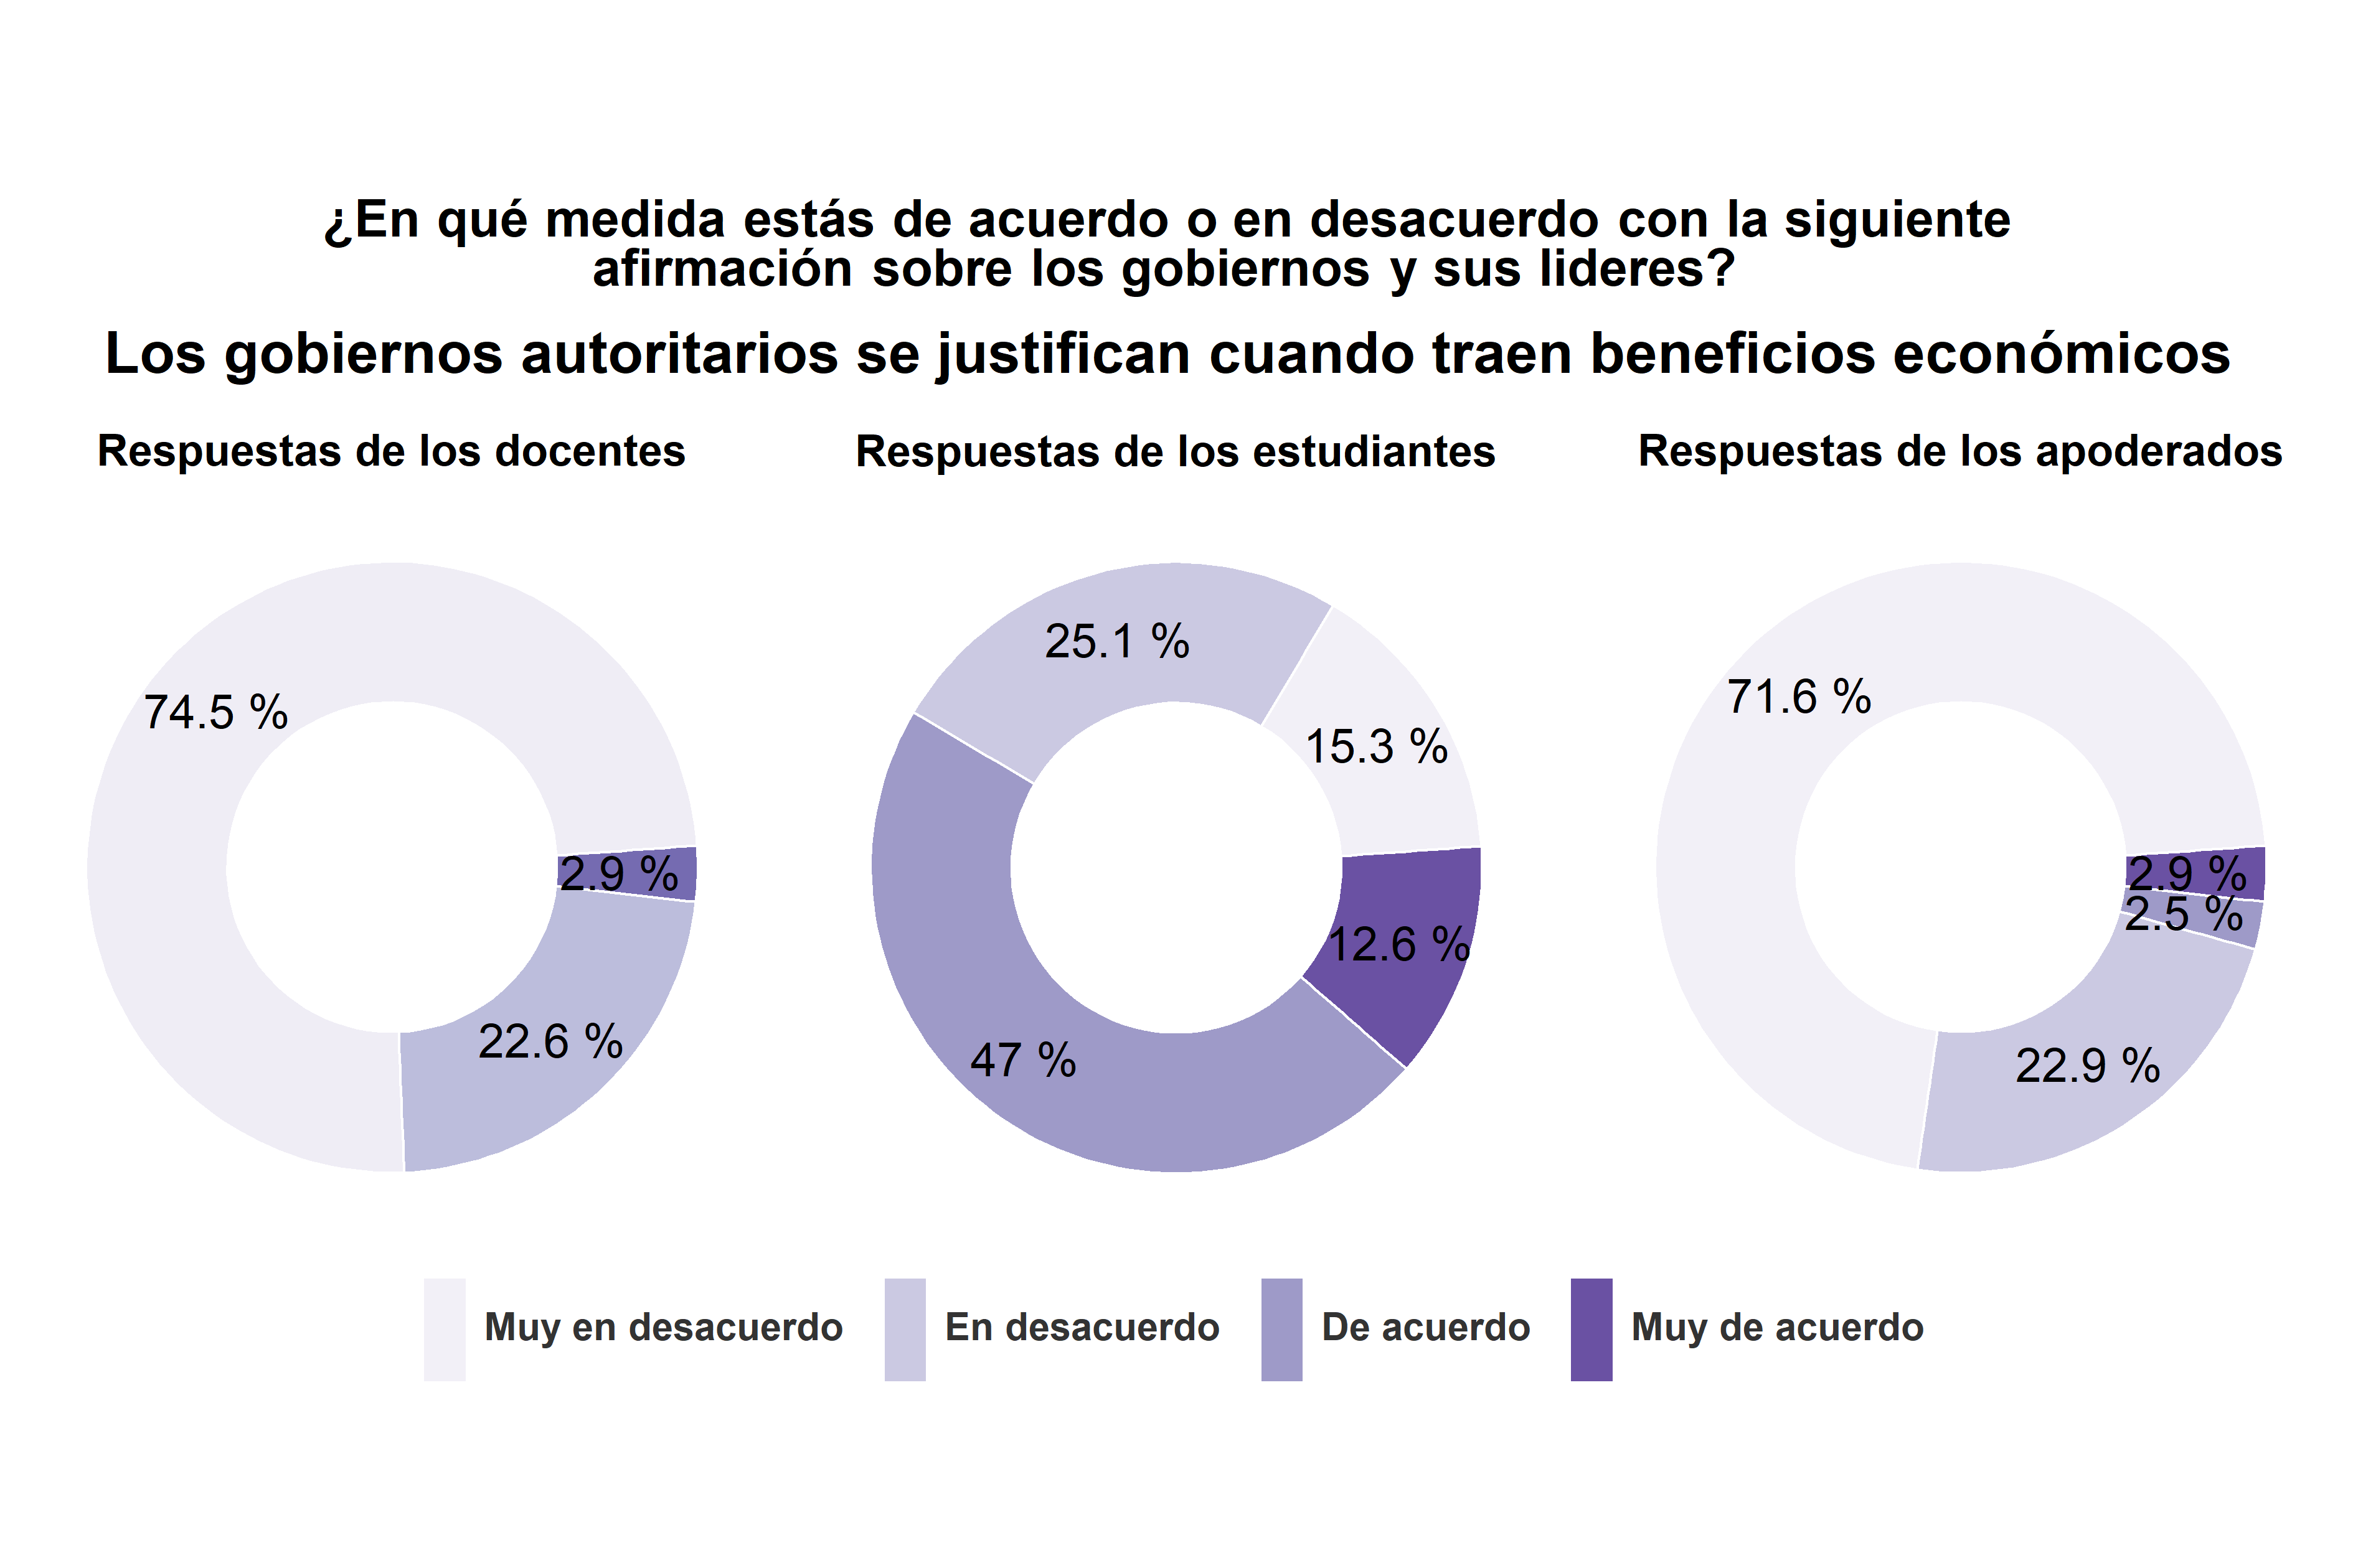
\includegraphics[width=52.49in]{images/graph_aut9} \end{center}

\hypertarget{secciuxf3n-3-confianza-en-instituciones}{%
\section{Sección 3: Confianza en instituciones}\label{secciuxf3n-3-confianza-en-instituciones}}

\begin{center}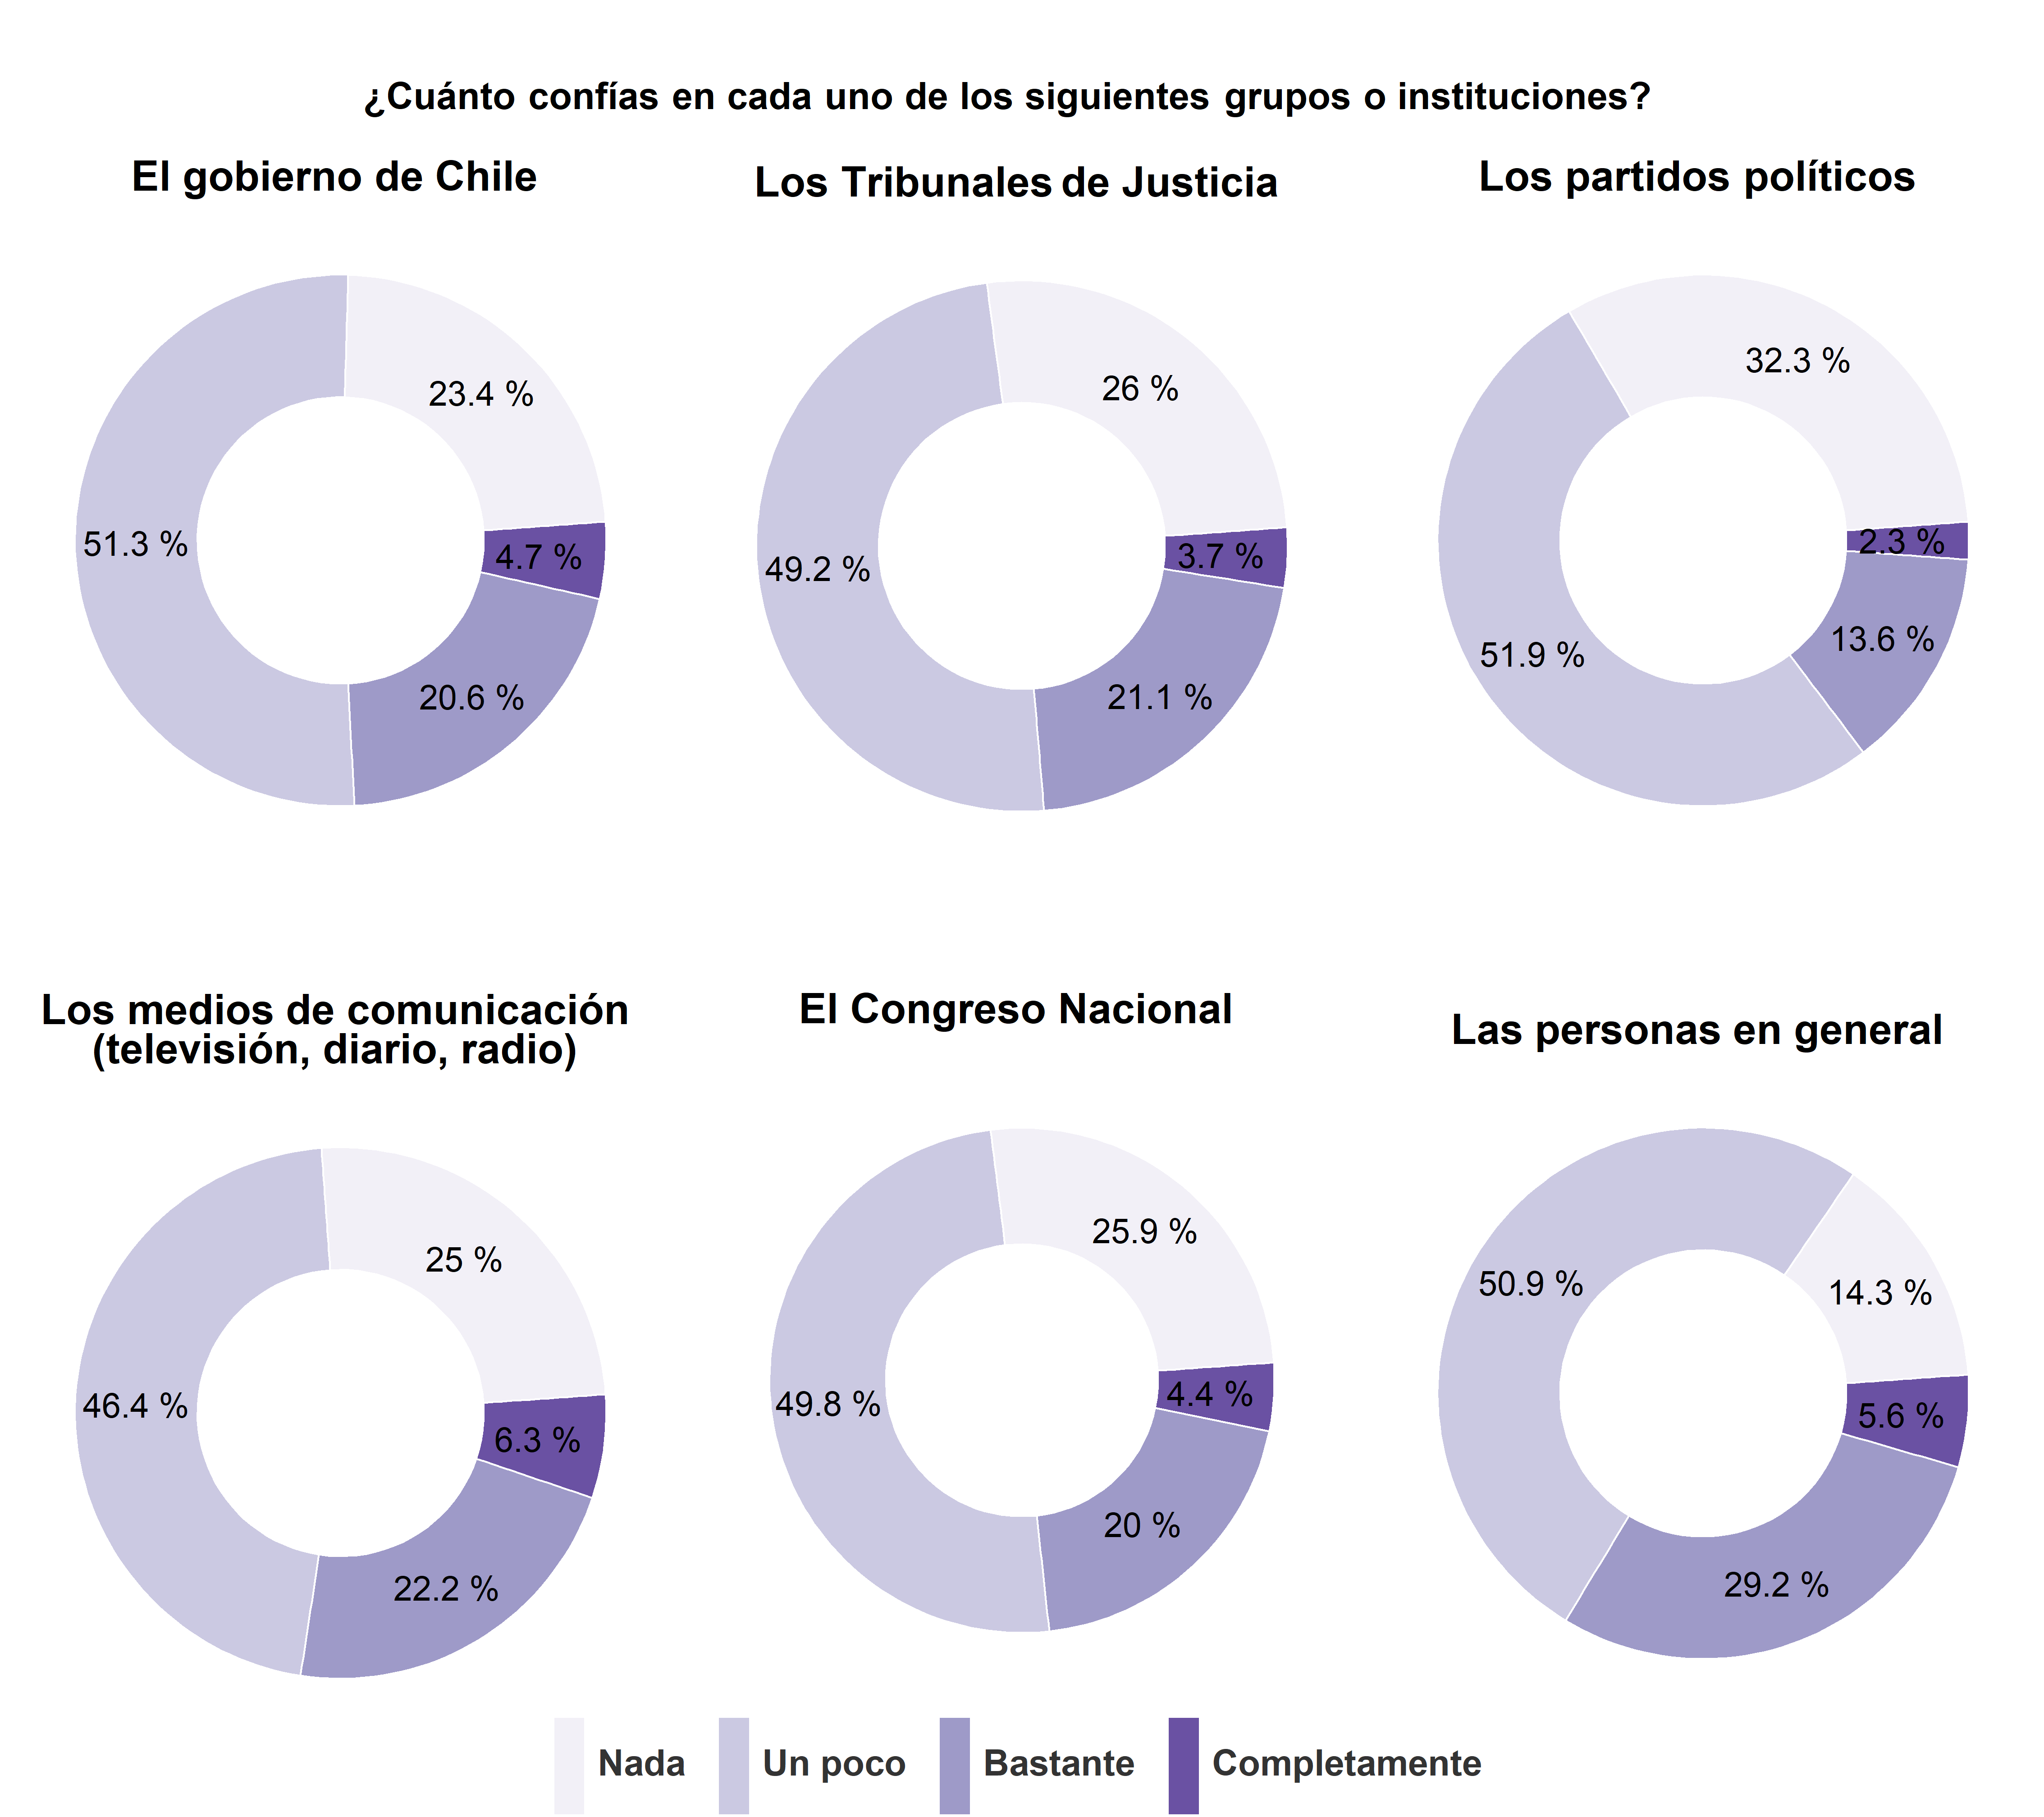
\includegraphics[width=62.99in]{images/graph_cgp} \end{center}

\hypertarget{participaciuxf3n}{%
\chapter{Participación}\label{participaciuxf3n}}

\hypertarget{secciuxf3n-1-participaciuxf3n-formal}{%
\section{Sección 1: Participación formal}\label{secciuxf3n-1-participaciuxf3n-formal}}

\begin{center}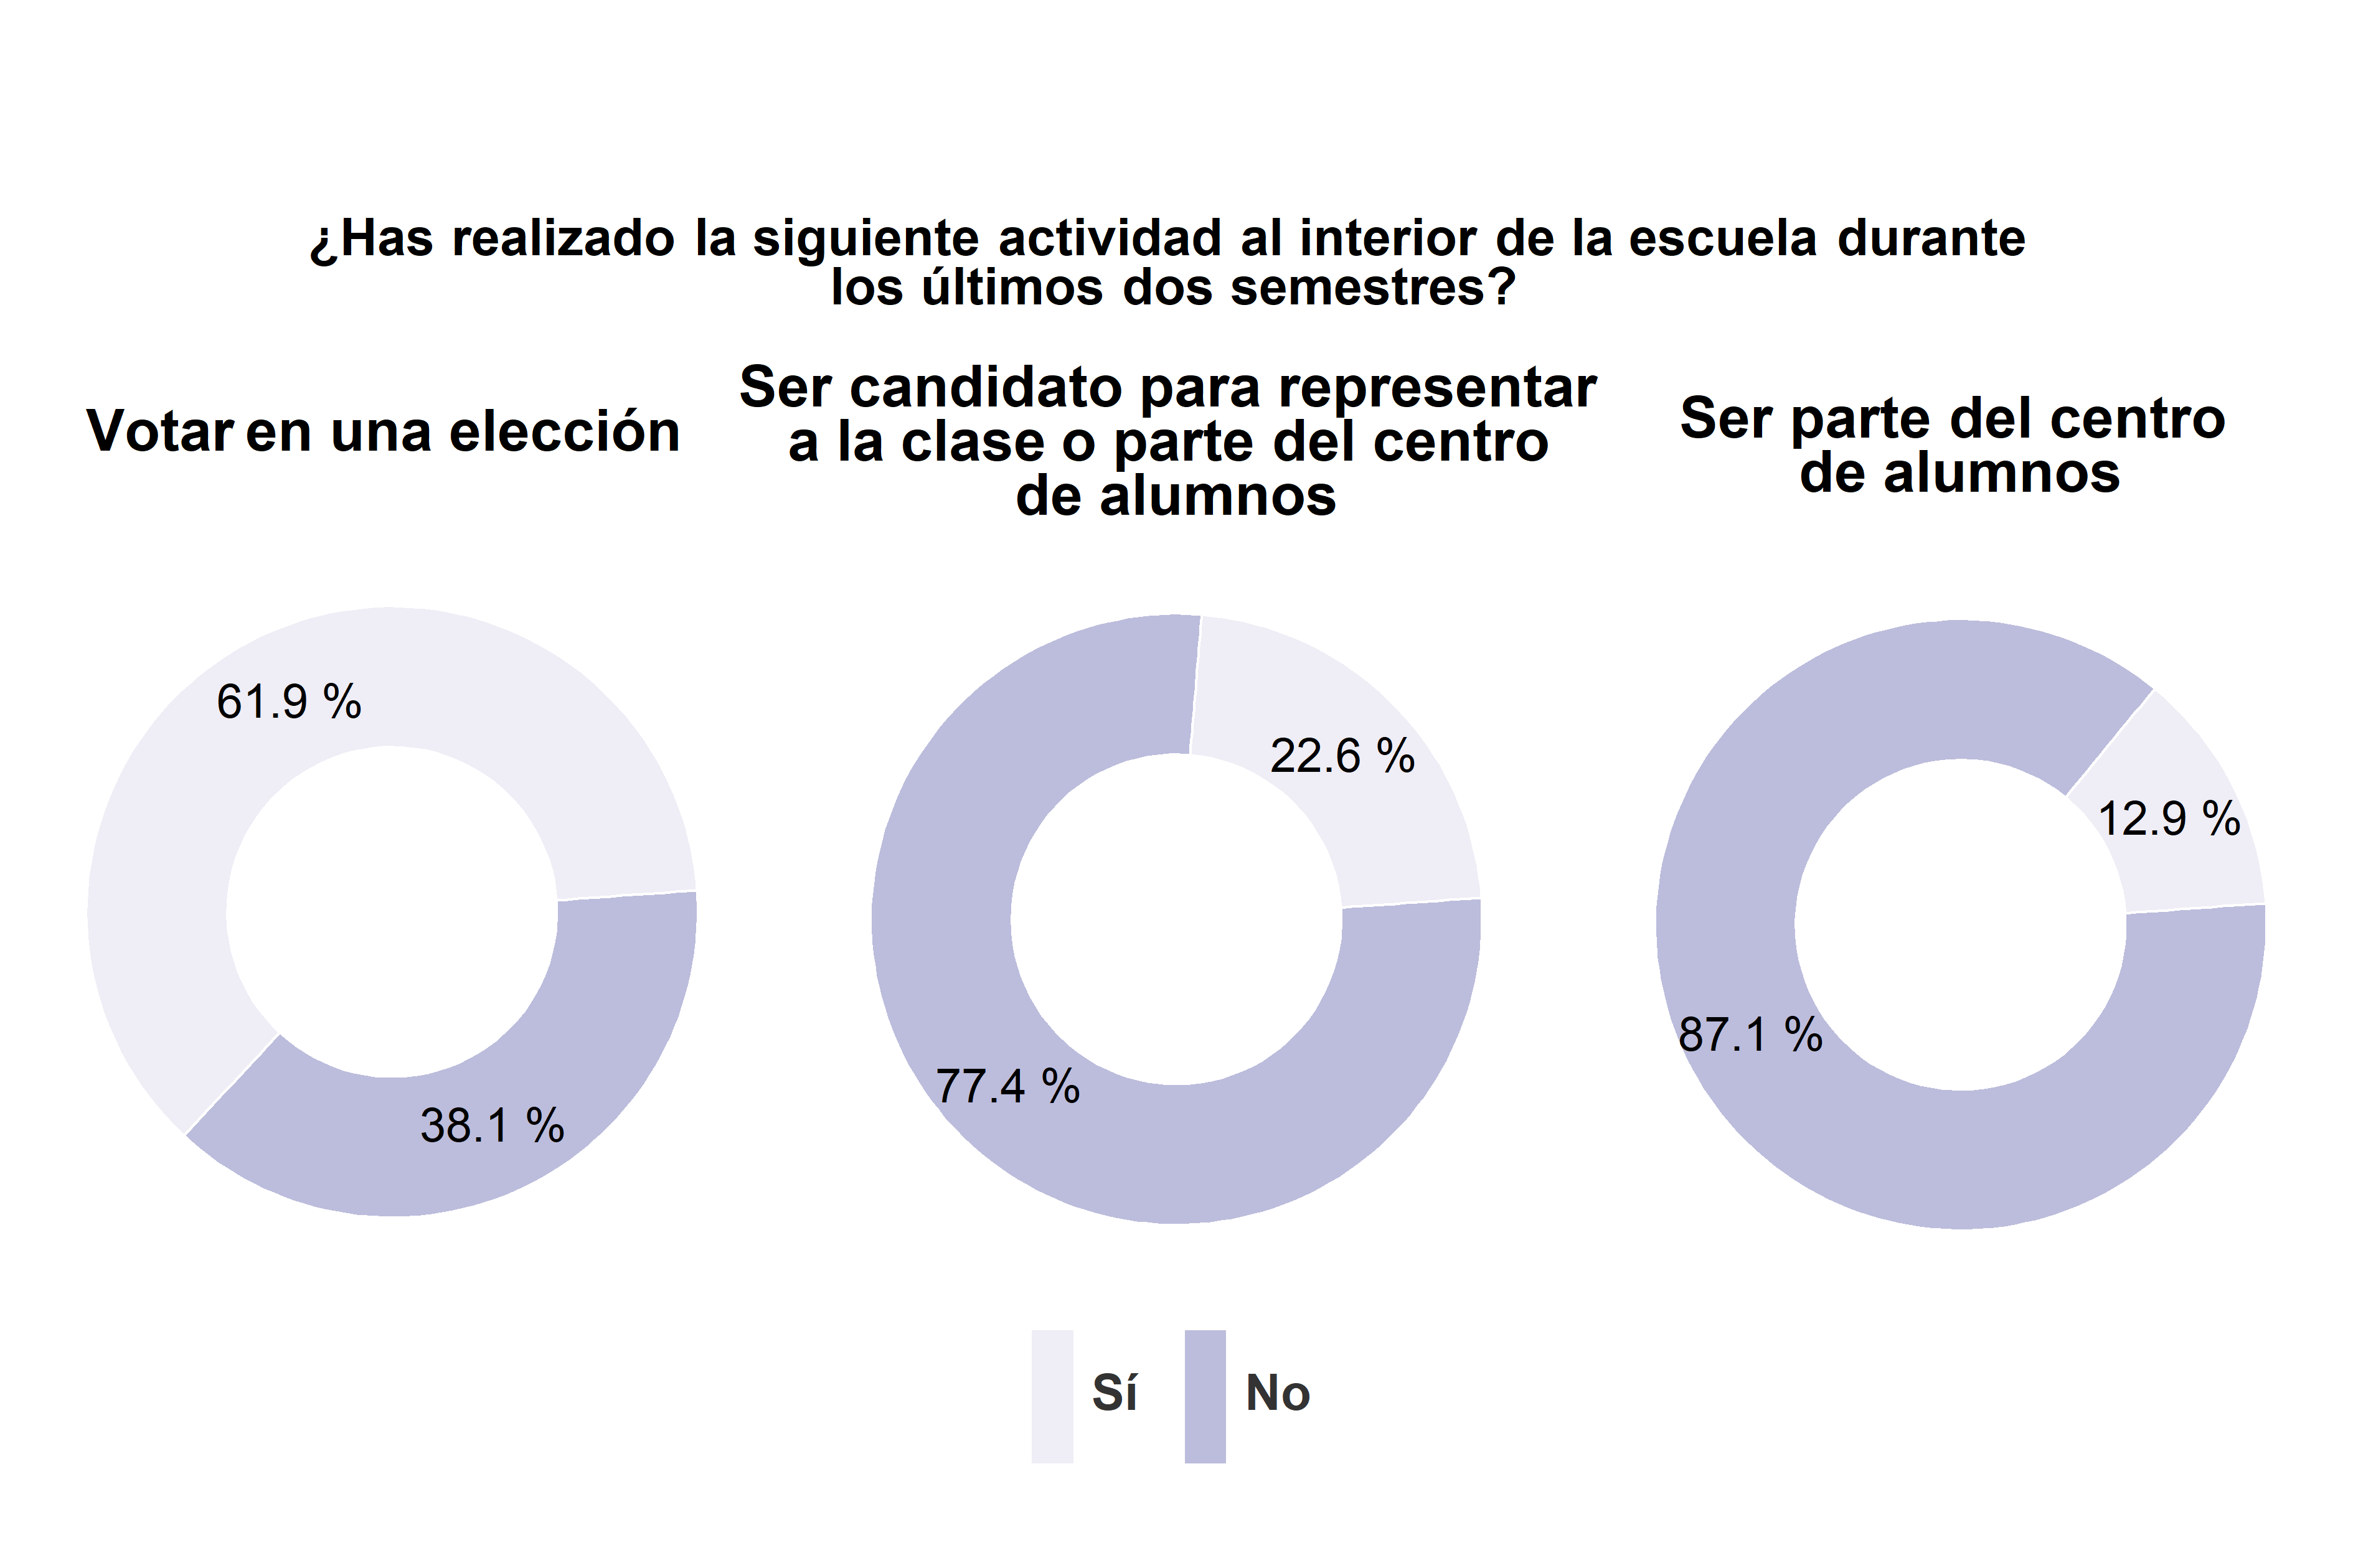
\includegraphics[width=52.49in]{images/graph_partform_act} \end{center}

\begin{center}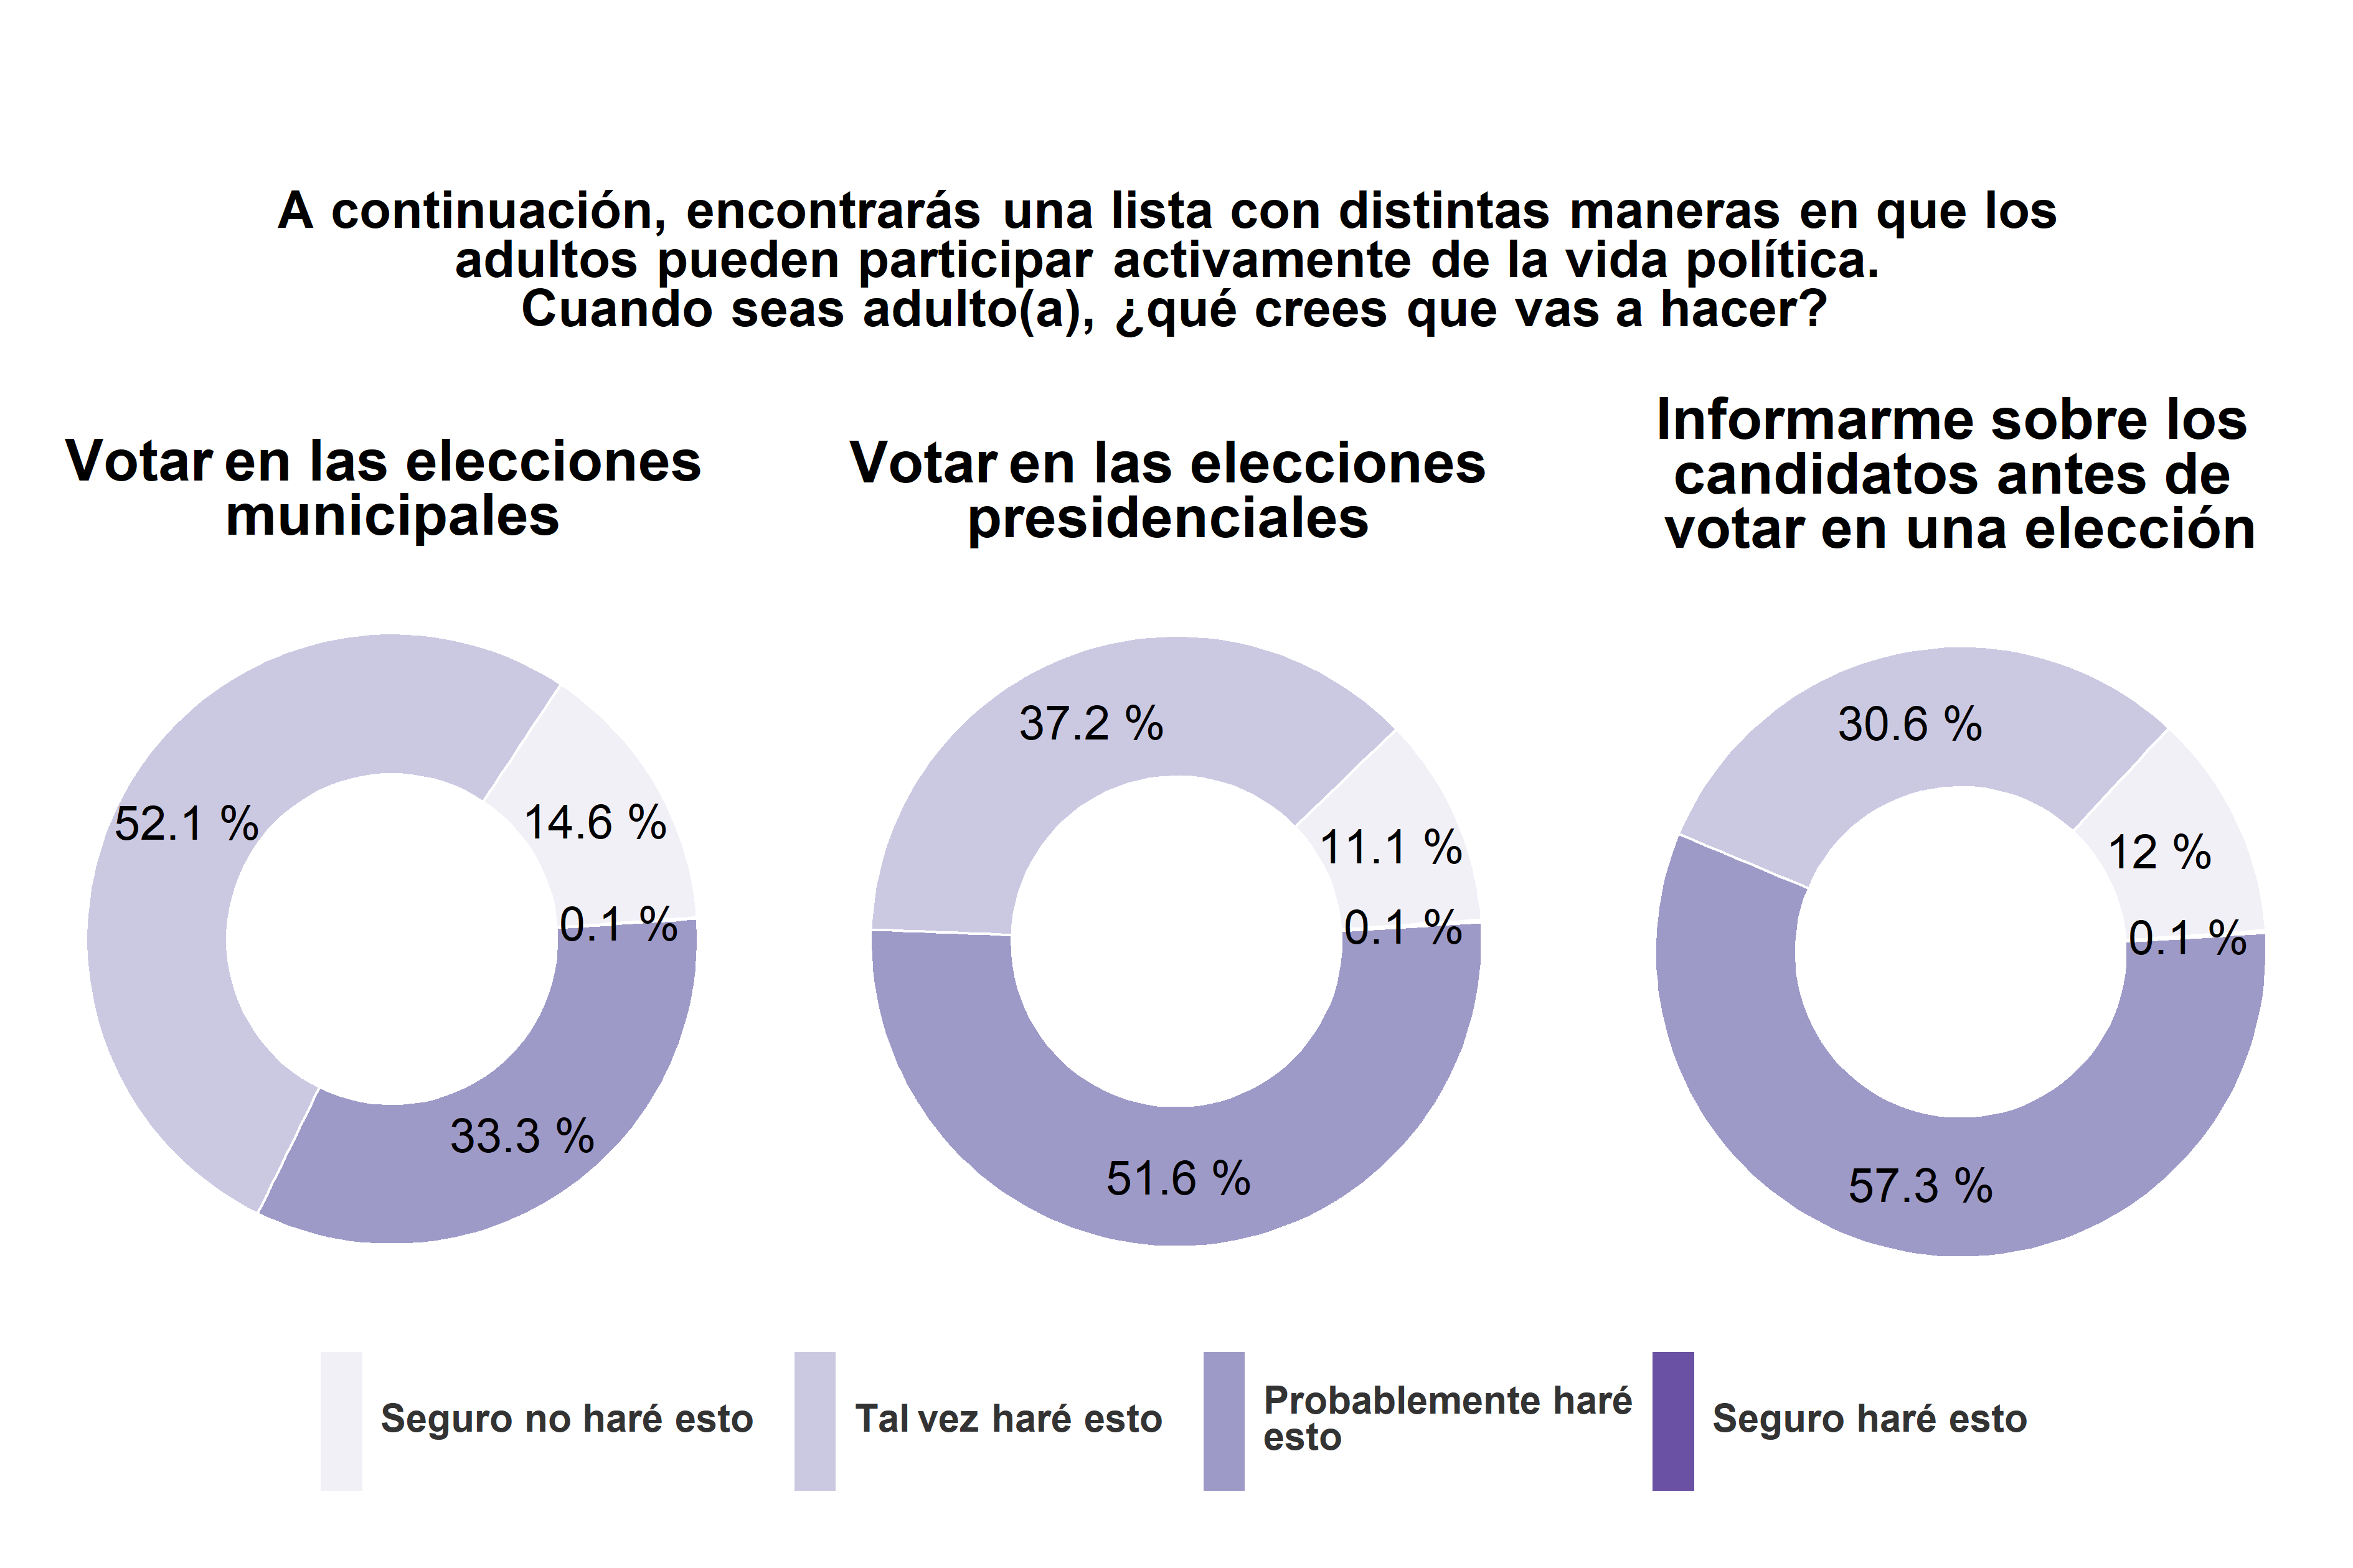
\includegraphics[width=52.49in]{images/graph_partform_fut} \end{center}

\hypertarget{secciuxf3n-2-participaciuxf3n-activista}{%
\section{Sección 2: Participación activista}\label{secciuxf3n-2-participaciuxf3n-activista}}

\begin{center}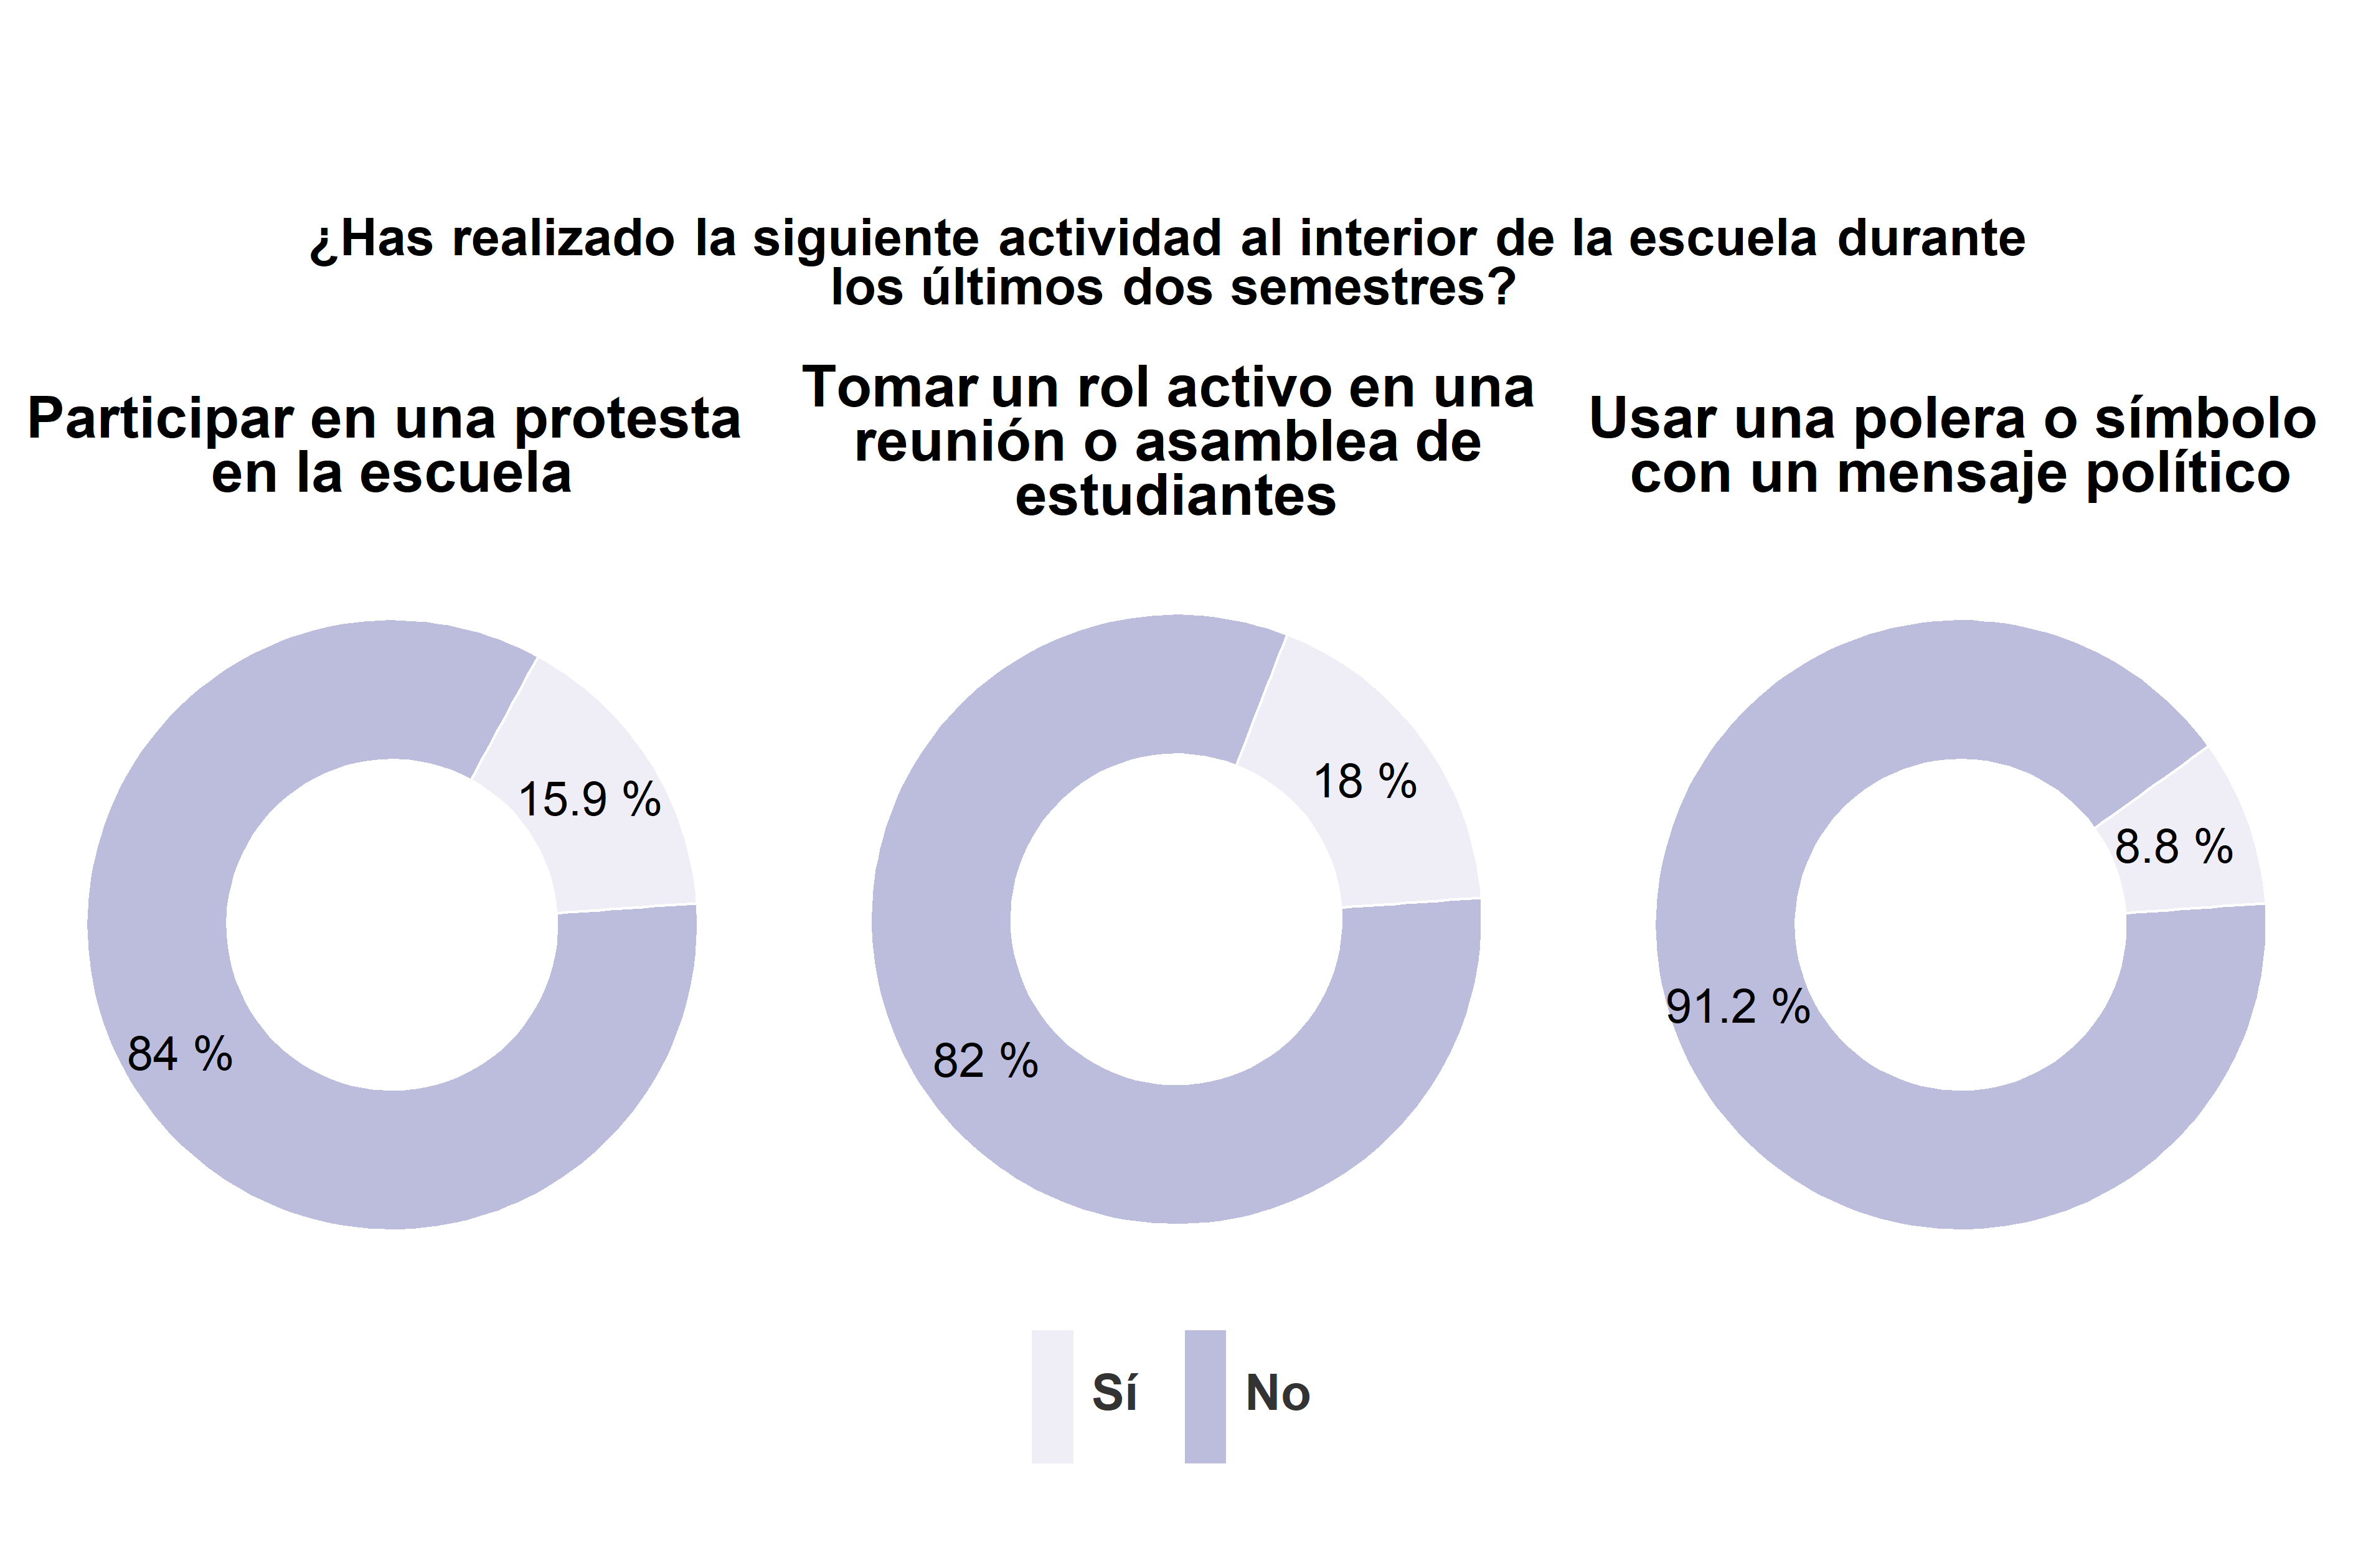
\includegraphics[width=52.49in]{images/graph_partact_esc} \end{center}

\begin{center}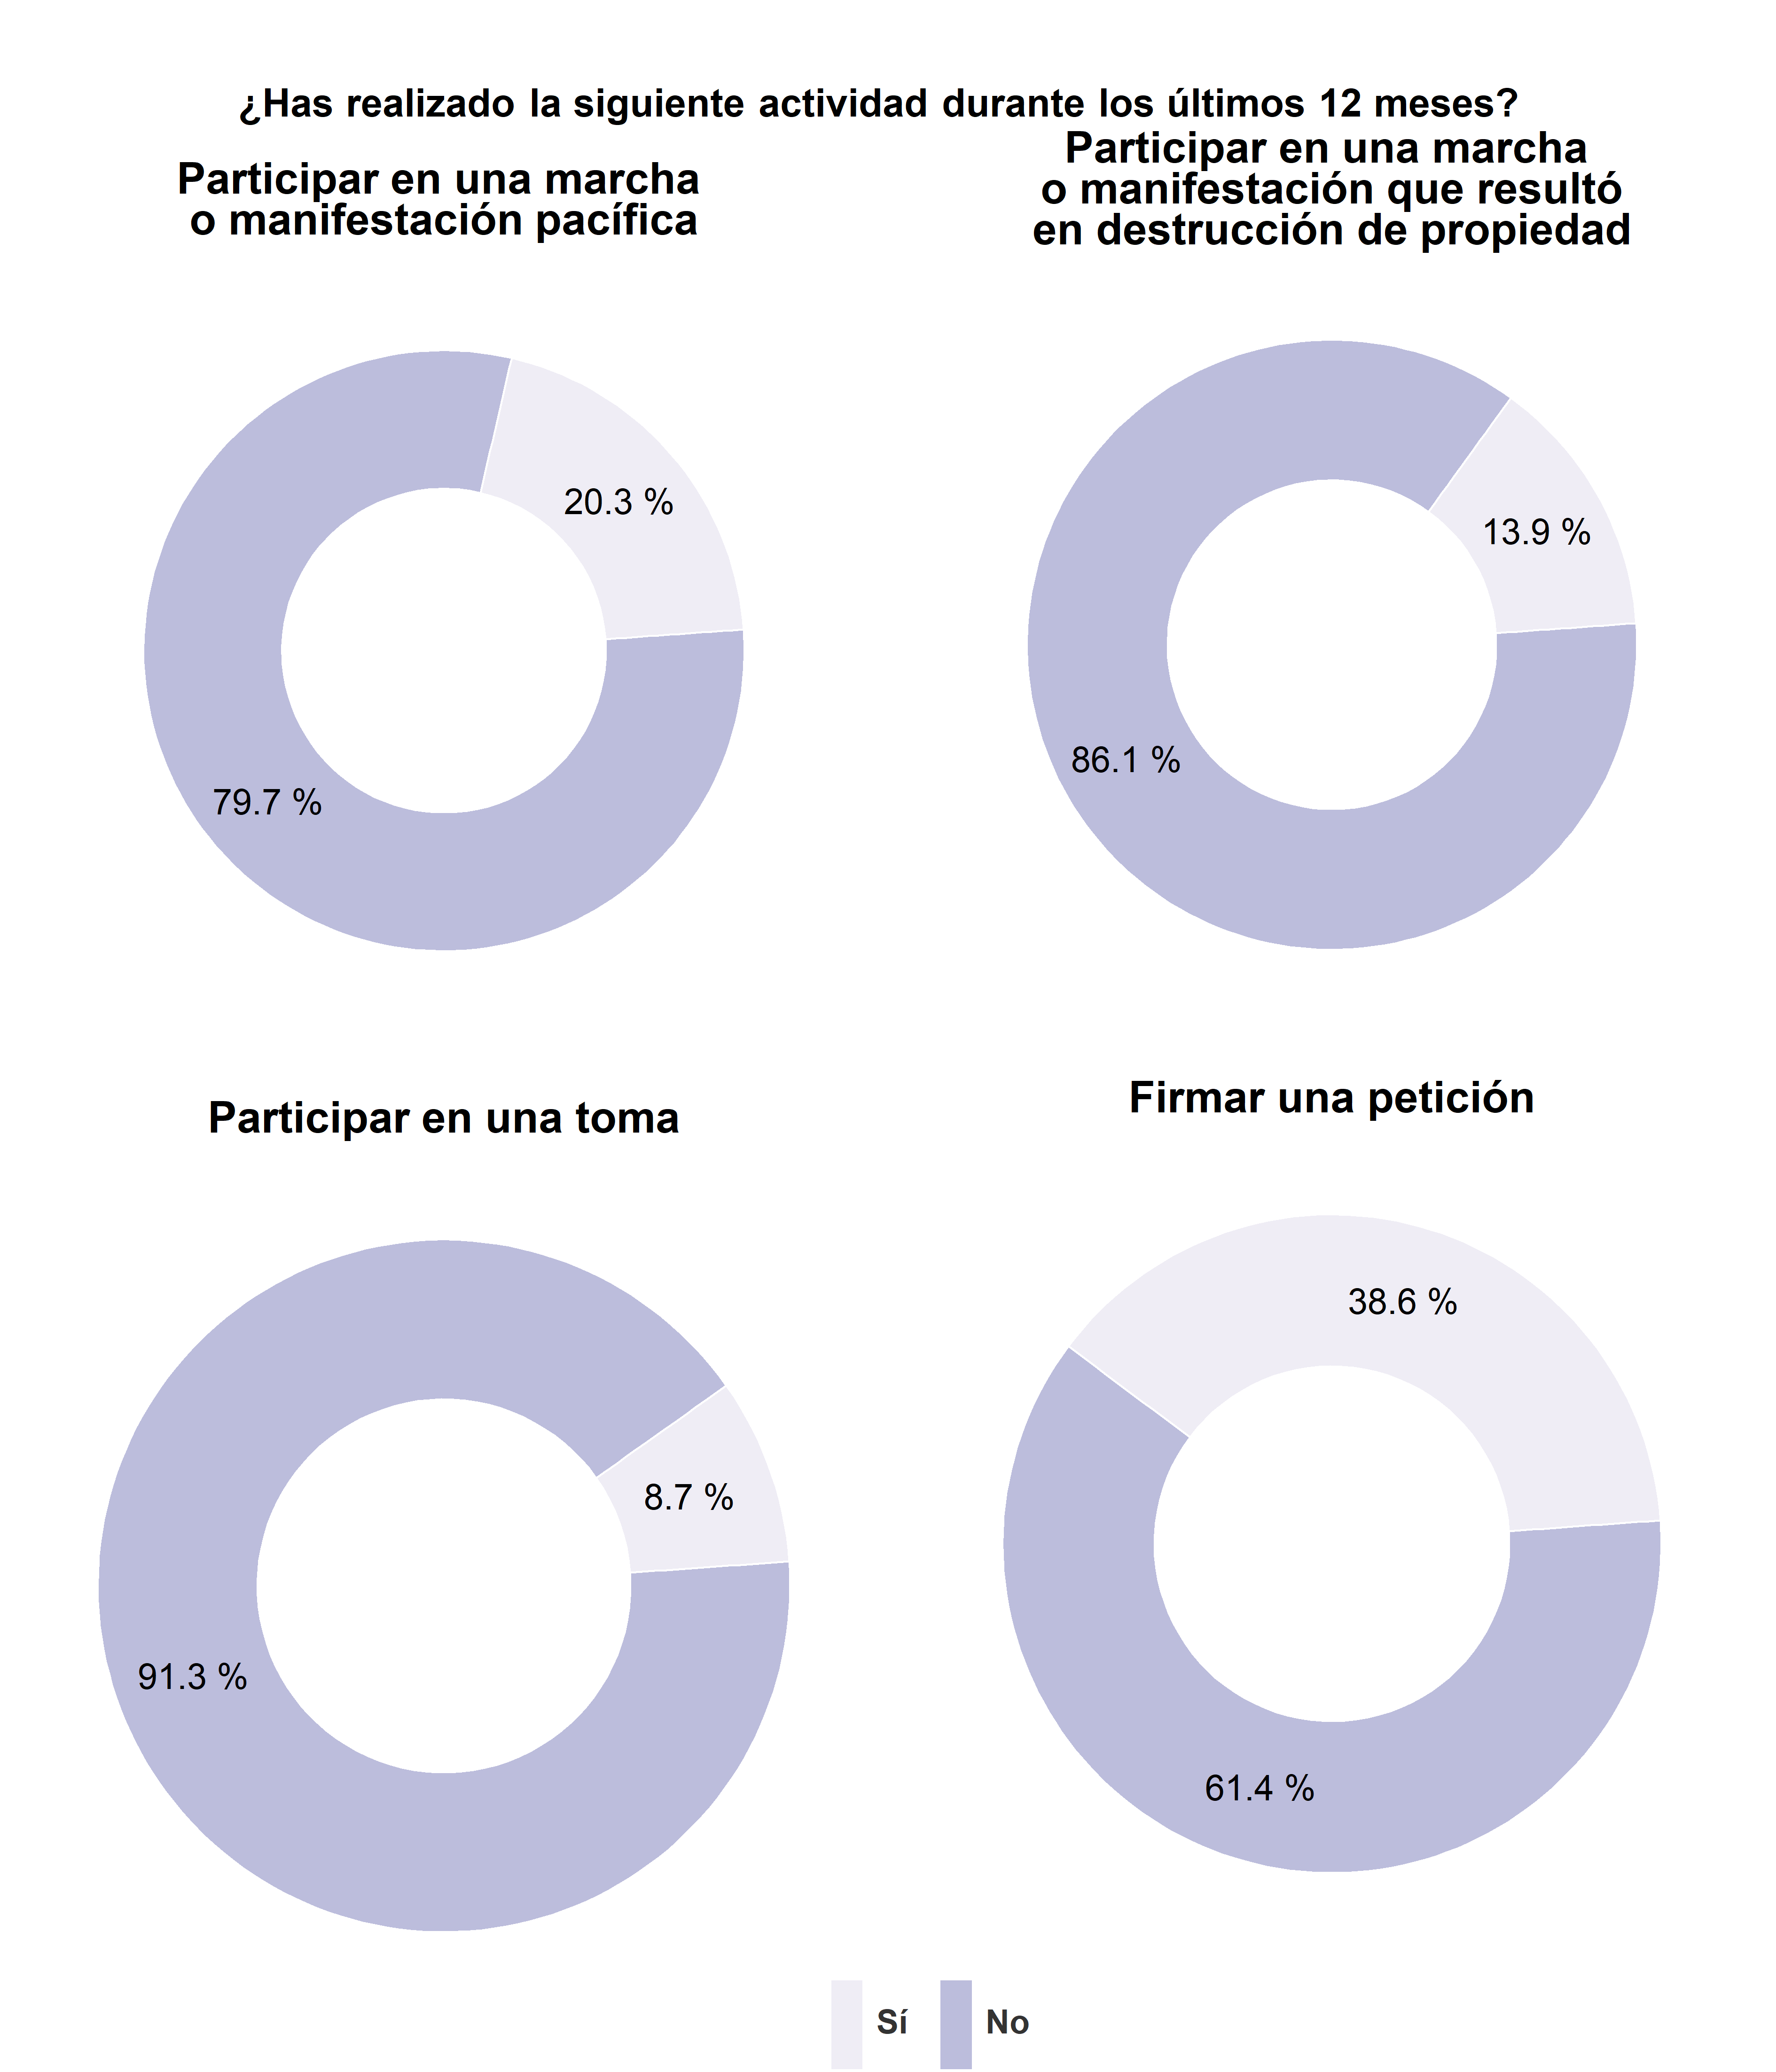
\includegraphics[width=52.49in]{images/graph_partact} \end{center}

\hypertarget{secciuxf3n-3-participaciuxf3n-comunitaria}{%
\section{Sección 3: Participación comunitaria}\label{secciuxf3n-3-participaciuxf3n-comunitaria}}

\begin{center}\includegraphics[width=52.49in]{images/graph_partcom_esc} \end{center}

\begin{center}\includegraphics[width=52.49in]{images/graph_partcom} \end{center}

  \bibliography{book.bib,packages.bib,openscience.bib}

\end{document}
